\documentclass[supercite]{Experimental_Report}

\title{~~~~~~数据结构实验~~~~~~}
\author{徐靖杰}
\school{计算机科学与技术学院}
\classnum{计算机类2505}
\stunum{U202514843}
\instructor{孙伟平}
\date{2026年6月15日}

\usepackage{algorithm, multirow}
\usepackage{algpseudocode}
\usepackage{amsmath}
\usepackage{amsthm}
\usepackage{framed}
\usepackage{mathtools}
\usepackage{subcaption}
\usepackage{xltxtra}
\usepackage{bm}
\usepackage{tikz}
\usepackage{tikzscale}
\usepackage{pgfplots}
\usepackage{titlesec}
\usepackage{listings}
\usepackage{xcolor}
\usepackage{fontspec}
\usepackage{microtype}
\usepackage{enumitem}
\usepackage[settings]{markdown}
\usetikzlibrary{shapes.multipart, shapes.geometric, arrows, positioning, 
                fit, chains, calc, backgrounds, arrows.meta}


\pgfplotsset{compat=1.16}

\definecolor{modernBackground}{RGB}{248, 249, 250}
\definecolor{modernFrame}{RGB}{208, 215, 222}
\definecolor{modernNumber}{RGB}{108, 117, 125}
\definecolor{modernKeyword}{RGB}{203, 36, 49}
\definecolor{modernString}{RGB}{0, 90, 156}
\definecolor{modernComment}{RGB}{106, 115, 125}
\definecolor{modernType}{RGB}{111, 66, 193}
\definecolor{modernFunction}{RGB}{34, 134, 58}
\definecolor{modernPreprocessor}{RGB}{183, 65, 14}
\definecolor{modernConstant}{RGB}{173, 127, 168}

\titleformat{\section}[block]{\centering\Large\bfseries}{\thesection}{1em}{}

\lstdefinestyle{elegantstyle}{
    language=C,
    basicstyle=\ttfamily\fontsize{9}{10}\selectfont,
    backgroundcolor=\color{modernBackground},
    keywordstyle=\color{modernKeyword}\bfseries,
    commentstyle=\color{modernComment}\itshape,
    stringstyle=\color{modernString},
    numbers=left,
    numberstyle=\tiny\color{modernNumber}\ttfamily,
    stepnumber=1,
    numbersep=8pt,
    frame=single,
    framesep=6pt,
    framerule=0.6pt,
    rulecolor=\color{modernFrame},
    frameround=tttt,
    breaklines=true,
    breakatwhitespace=true,
    breakautoindent=true,
    breakindent=15pt,
    showstringspaces=false,
    tabsize=3,
    captionpos=b,
    abovecaptionskip=8pt,
    belowcaptionskip=8pt,
    xleftmargin=12pt,
    xrightmargin=12pt,
    escapeinside={/*@}{@*/},
    morekeywords={size_t, bool, true, false, status, ElemType, LinkList, LNode, NamedList, LISTS, VertexType, ArcNode, VNode, AdjList, ALGraph, GraphKind, NamedGraph, GRAPHS, KeyType, HANDLE, STD_OUTPUT_HANDLE, FILE},
    emphstyle={\color{modernConstant}},
}

\lstset{
    style=elegantstyle,
    emph={char, int, float, double, void, short, long, signed, unsigned, const, static, extern, register, auto, volatile, restrict, inline, typedef, struct, enum},
    emphstyle={\color{modernType}\bfseries},
    morecomment=[l][\color{modernPreprocessor}]{\#},
}

\algnewcommand\Null{\textsc{null }}
\algnewcommand\algorithmicinput{\textbf{Input:}}
\algnewcommand\Input{\item[\algorithmicinput]}
\algnewcommand\algorithmicoutput{\textbf{Output:}}
\algnewcommand\Output{\item[\algorithmicoutput]}
\algnewcommand{\LeftCom}[1]{\State $\triangleright$ #1}

\colorlet{shadecolor}{black!15}

% ---- shared TikZ styles (compact to avoid overflow) ----
\tikzset{
  flowStart/.style={rectangle, rounded corners, minimum width=1.8cm, minimum height=0.5cm, align=center, draw=black, fill=red!20, font=\tiny, inner sep=2pt},
  flowProc/.style={rectangle, minimum width=1.8cm, minimum height=0.5cm, align=center, draw=black, fill=blue!20, font=\tiny, inner sep=2pt},
  flowDec/.style={diamond, aspect=2.2, minimum width=1.6cm, minimum height=0.65cm, align=center, draw=black, fill=green!20, font=\tiny, inner sep=0pt},
  flowArr/.style={thick,->,>=Stealth, font=\tiny},
}

\begin{document}

\maketitle
\clearpage
\pagenumbering{Roman}
\tableofcontents
\clearpage
\pagenumbering{arabic}

%==========================================================================
\section{实验二\quad 线性表综合管理系统}
%==========================================================================

\subsection{实验目的与要求}

\subsubsection{实验目的}

\begin{enumerate}
    \item 深入理解线性表的链式存储结构——单链表的原理与实现方法
    \item 掌握单链表的基本操作：初始化、销毁、清空、判空、求长、取值、查找、前驱后继、插入、删除、遍历
    \item 掌握单链表的高级操作：逆置、删除倒数第N个节点、排序、文件读写
    \item 理解多表管理的数据组织方式，掌握基于名称索引的线性表集合管理
    \item 熟练运用指针操作和动态内存管理，培养系统化编程思维
\end{enumerate}

\subsubsection{实验要求}
设计并实现一个线性表综合管理系统：单表模式（18项操作）+ 多表模式（创建/选择/删除命名线性表）。
基本操作涵盖初始化、销毁、清空、判空、求长度、按位取值、按值查找、求前驱后继、插入删除、遍历输出；
高级操作包括逆置、删除倒数第N个节点、冒泡排序、文件持久化。

\subsection{系统总体设计}

\subsubsection{数据结构设计——三层数据模型}

\begin{enumerate}
    \item \textbf{LNode（链表节点）}：底层数据单元，含\texttt{ElemType data}和\texttt{struct LNode *next}
    \item \textbf{NamedList（命名线性表）}：中间层，将链表指针\texttt{L}与字符串名称\texttt{name[20]}绑定
    \item \textbf{LISTS（线性表集合）}：顶层容器，管理最多10个命名线性表，\texttt{length}记录数量
\end{enumerate}

\begin{figure}[!htb]
\centering\footnotesize
\begin{tikzpicture}[
    box/.style={rectangle, minimum width=2.8cm, minimum height=0.65cm, align=center, draw=black, rounded corners, font=\scriptsize},
    sbox/.style={rectangle, minimum width=2.5cm, minimum height=0.55cm, align=center, draw=black, font=\tiny},
    arrow/.style={thick,->,>=Stealth}
]
\node (lists) [box, fill=red!15] {\textbf{LISTS} (全局变量 lists)};
\node [font=\tiny, below=0.1cm of lists] {length = 2};
\node (nl0) [box, fill=blue!10, below left=0.8cm and -1.2cm of lists] {NamedList[0]\\name = "ListA"};
\node (nl1) [box, fill=blue!10, below=0.15cm of nl0] {NamedList[1]\\name = "ListB"};
\node (head0) [sbox, fill=green!10, right=0.8cm of nl0] {头节点};
\node (n0a) [sbox, fill=yellow!15, right=0.3cm of head0] {data: 5};
\node (n0b) [sbox, fill=yellow!15, right=0.3cm of n0a] {data: 3};
\node [right=0.3cm of n0b, font=\tiny] {NULL};
\draw [arrow] (nl0.east) -- (head0.west);
\draw [arrow] (head0.east) -- (n0a.west);
\draw [arrow] (n0a.east) -- (n0b.west);
\draw [arrow, dashed, gray] (lists.south) -- (nl0.north);
\draw [arrow, dashed, gray] (lists.south) -- (nl1.north);
\end{tikzpicture}
\caption{数据结构层次关系示意图}
\label{fig:ds-hierarchy}
\end{figure}

\subsubsection{系统架构——三层模块化设计}

% Mermaid 参考: 图2 (核心数据结构关系图) — 见 Mermaid流程图.txt
\begin{itemize}
    \item \textbf{数据层}：LNode / NamedList / LISTS 三级结构
    \item \textbf{操作层}：16个链表操作函数 + 4个多表管理函数
    \item \textbf{交互层}：菜单驱动、彩色输出（Windows Console API）、用户输入解析
\end{itemize}

核心设计理念是\textbf{关注点分离}：修改菜单布局不影响算法实现，优化算法不影响界面代码，新增功能只需在操作层添加函数并在交互层注册菜单项。

% Mermaid 参考: 图1 (系统三层架构) — 见 Mermaid流程图.txt
\subsection{基本功能函数分析}

以下按照数据结构实验任务书的规格，对线性表12个基本操作函数逐一给出函数原型、初始条件、操作结果和实现分析。

\subsubsection{InitList(L)——初始化表}
% Mermaid 参考: 图4 (InitList) — 见 Mermaid流程图.txt

\begin{quote}\small
\textbf{初始条件：}线性表L不存在。\quad\textbf{操作结果：}构造一个空的线性表。
\end{quote}

实现分析：通过\texttt{malloc}分配一个LNode作为头节点（哨兵节点），将\texttt{next}置空。头节点的引入使得空表和非空表可以使用统一的插入、删除逻辑。函数首先检查\texttt{*L != NULL}防止重复初始化。

\begin{lstlisting}[label={lst:init}, caption={InitList}]
status InitList(LinkList *L) {
    if (*L != NULL) return INFEASIBLE;
    LinkList t = (LinkList)malloc(sizeof(LNode));
    if (t == NULL) return OVERFLOW;
    t->next = NULL;
    *L = t;
    return OK;
}
\end{lstlisting}



\subsubsection{DestroyList(L)——销毁表}


\begin{quote}\small
\textbf{初始条件：}线性表L已存在。\quad\textbf{操作结果：}销毁线性表L，释放包括头节点在内的所有节点。
\end{quote}

实现分析：使用"边遍历边释放"策略，变量p预先记录下一个节点地址再释放当前节点（\texttt{p = (*L)->next; free(*L); *L = p;}）。最后显式置NULL防止野指针。时间复杂度$O(n)$。

\begin{lstlisting}[label={lst:destroy}, caption={DestroyList}]
status DestroyList(LinkList *L) {
    if (*L == NULL) return INFEASIBLE;
    LinkList p = *L;
    while (*L != NULL) {
        p = (*L)->next;
        free(*L);
        *L = p;
    }
    *L = NULL;
    return OK;
}
\end{lstlisting}

\subsubsection{ClearList(L)——清空表}
% Mermaid 参考: 图6 (ClearList) — 见 Mermaid流程图.txt

\begin{quote}\small
\textbf{初始条件：}线性表L已存在。\quad\textbf{操作结果：}将L重置为空表（保留头节点）。
\end{quote}

实现分析：与DestroyList的关键区别——ClearList从\texttt{(*L)->next}开始释放仅释放数据节点，保留头节点。清空后\texttt{(*L)->next = NULL}，链表恢复空表状态。时间复杂度$O(n)$。

\begin{lstlisting}[label={lst:clear}, caption={ClearList}]
status ClearList(LinkList *L) {
    if (*L == NULL) return INFEASIBLE;
    LinkList p = (*L)->next;
    LinkList q = (*L)->next;
    while (q != NULL) { p = q->next; free(q); q = p; }
    (*L)->next = NULL;
    return OK;
}
\end{lstlisting}
\begin{figure}[!htb]
	\centering
	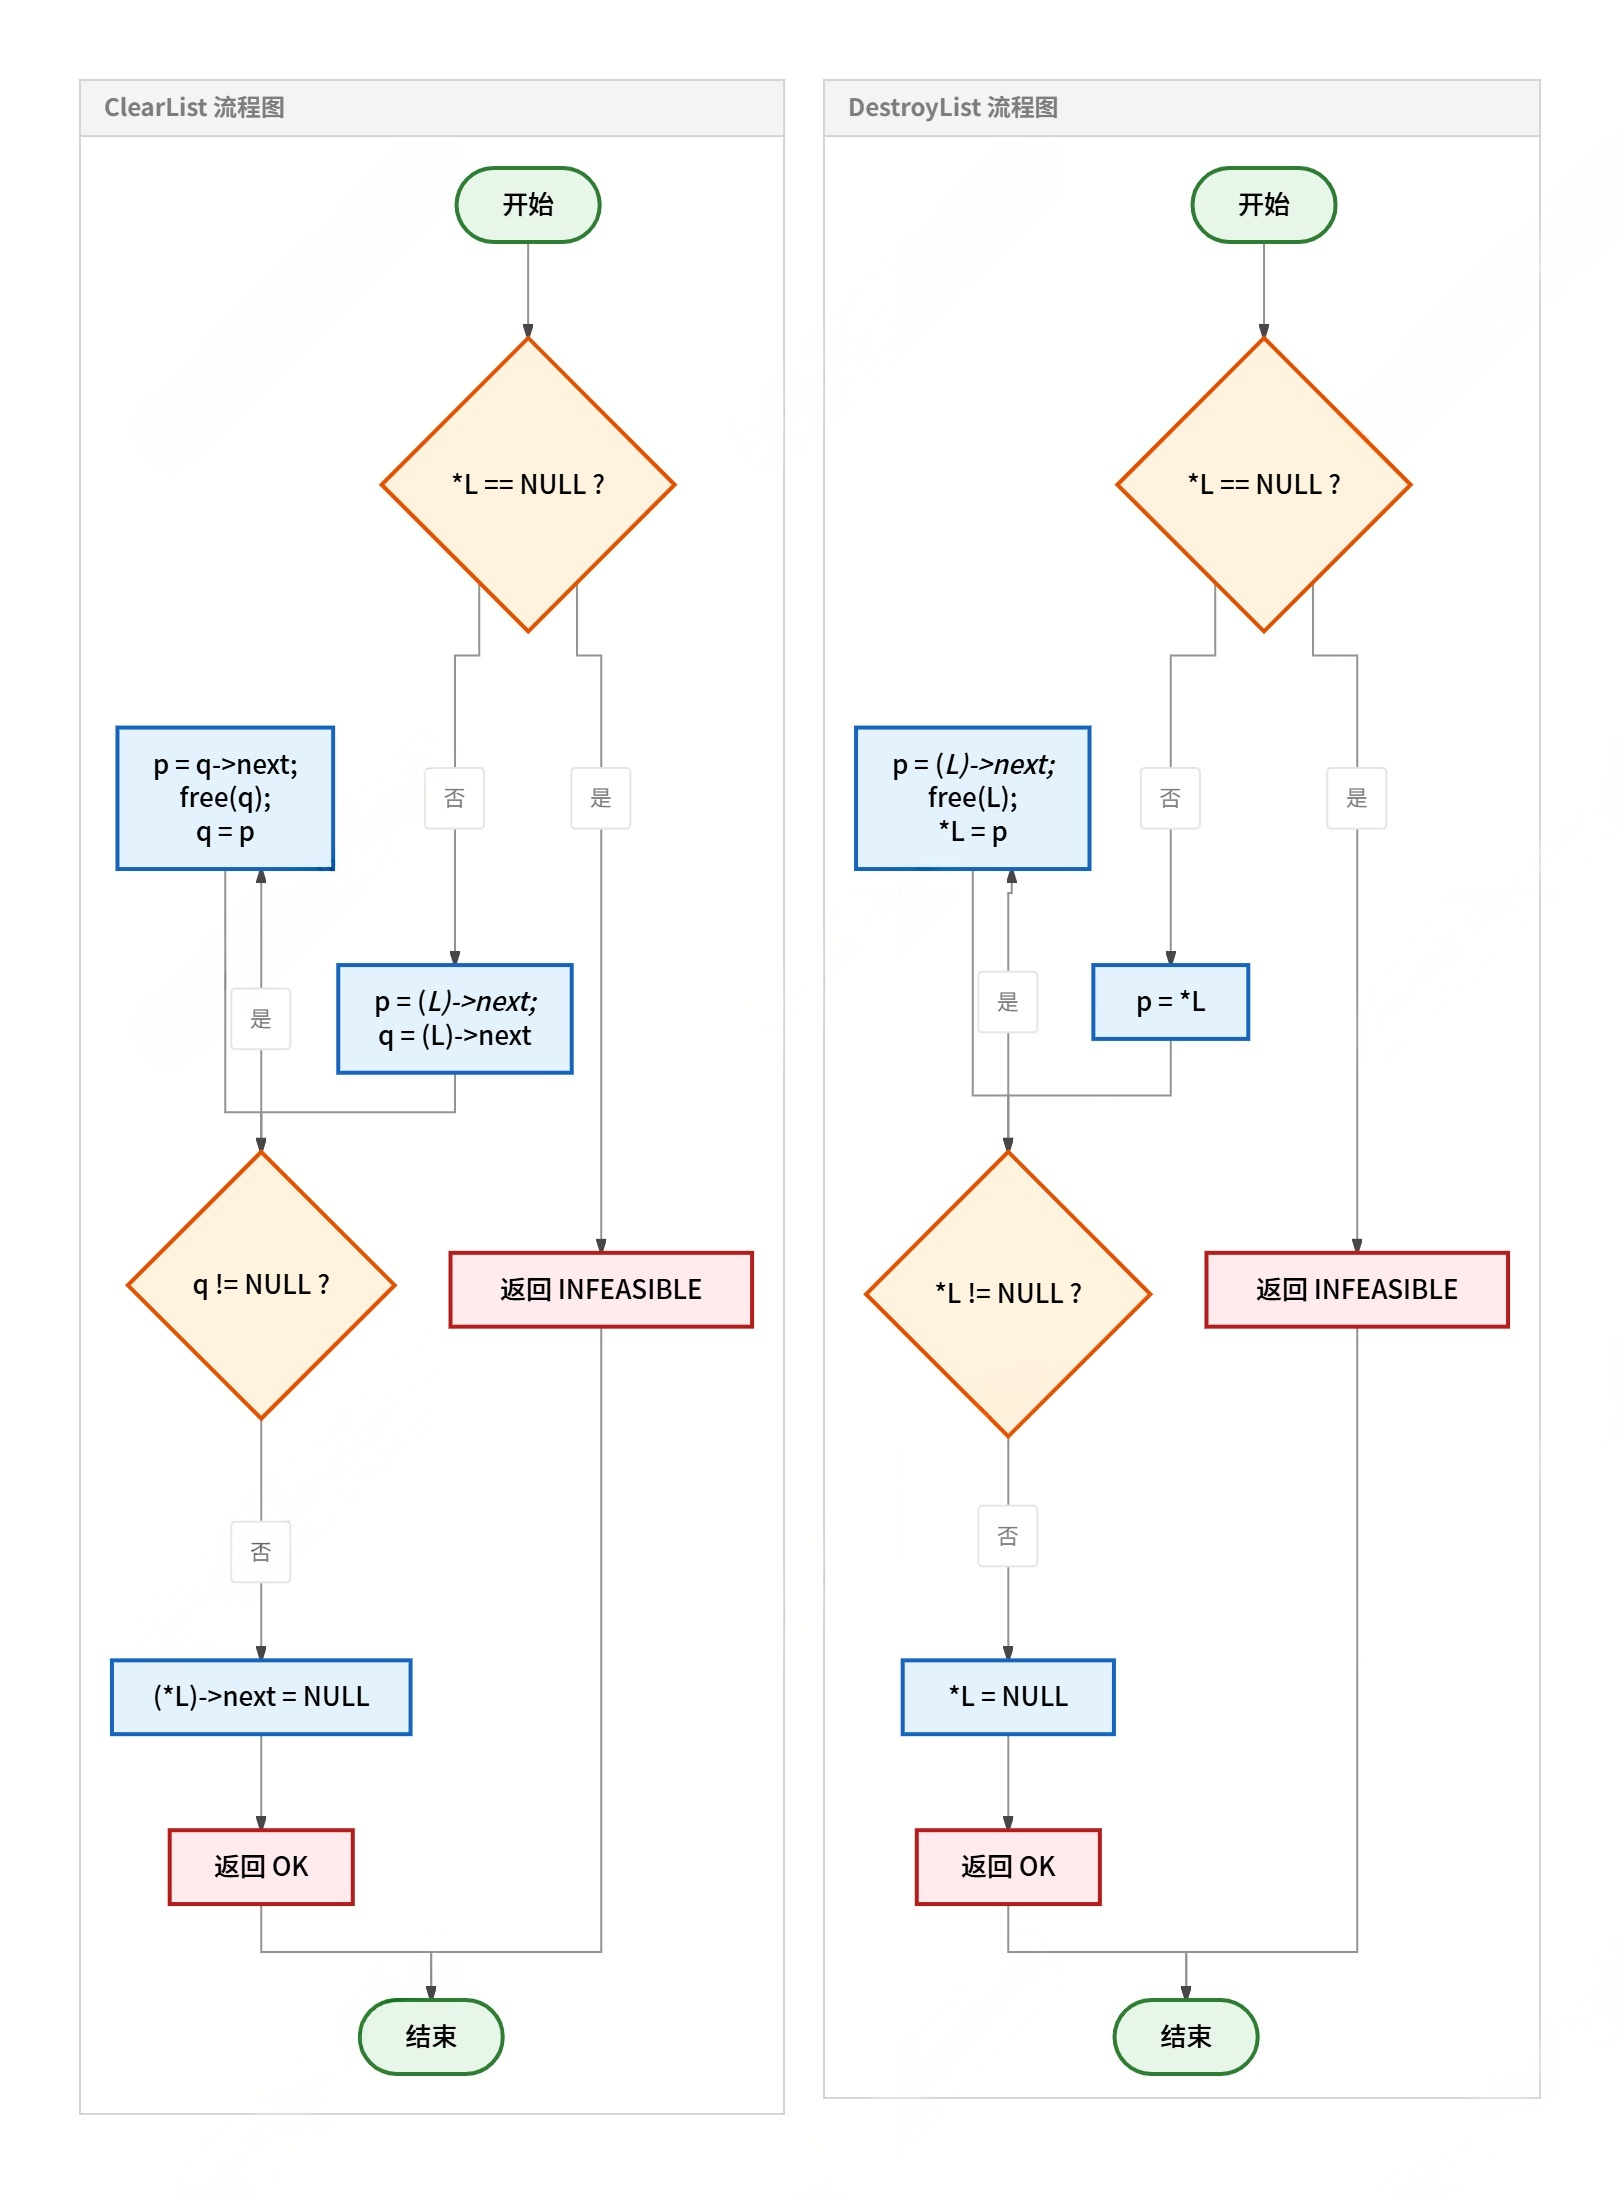
\includegraphics[width=\linewidth]{Destroy Clear对比.png}
	\caption{Destroy Clear 对比图}
\end{figure}
\subsubsection{ListEmpty(L)——判定空表}
% Mermaid 参考: 图7 (ListEmpty) — 见 Mermaid流程图.txt

\begin{quote}\small
\textbf{初始条件：}线性表L已存在。\quad\textbf{操作结果：}若L为空表返回TRUE，否则返回FALSE。
\end{quote}

实现分析：通过\texttt{L->next == NULL}判断是否有数据节点。先检查L本身是否为NULL（表不存在）。时间复杂度$O(1)$。

\begin{lstlisting}[label={lst:empty}, caption={ListEmpty}]
status ListEmpty(LinkList L) {
    if (L == NULL) return INFEASIBLE;
    return (L->next == NULL) ? TRUE : FALSE;
}
\end{lstlisting}

\subsubsection{ListLength(L)——求表长}
% Mermaid 参考: 图8 (ListLength) — 见 Mermaid流程图.txt

\begin{quote}\small
\textbf{初始条件：}线性表L已存在。\quad\textbf{操作结果：}返回L中数据元素的个数。
\end{quote}

实现分析：遍历链表计数，由于含头节点，最终\texttt{cnt - 1}得到数据节点数量。时间复杂度$O(n)$——链式存储无法像顺序表那样$O(1)$获取长度。

\begin{lstlisting}[label={lst:len}, caption={ListLength}]
int ListLength(LinkList L) {
    int cnt = 0;
    if (L == NULL) return INFEASIBLE;
    while (L != NULL) { cnt++; L = L->next; }
    return cnt - 1;
}
\end{lstlisting}

\subsubsection{GetElem(L, i, e)——获得元素}
% Mermaid 参考: 图9 (GetElem) — 见 Mermaid流程图.txt

\begin{quote}\small
\textbf{初始条件：}线性表L已存在，$1\leq i\leq\text{ListLength}(L)$。\quad\textbf{操作结果：}用e返回L中第i个数据元素的值。
\end{quote}

实现分析：从头节点后继（第1个数据节点）开始，计数器cnt=1同步递增，当cnt==i时通过*e返回数据。需处理三种异常：表不存在、空表、i超出范围。时间复杂度$O(n)$。

\begin{lstlisting}[label={lst:getelem}, caption={GetElem}]
status GetElem(LinkList L, int i, ElemType *e) {
    if (L == NULL) return INFEASIBLE;
    if (L->next == NULL) return ERROR;
    int cnt = 0;
    L = L->next;
    while (L != NULL) {
        cnt++;
        if (cnt == i) { *e = L->data; return OK; }
        L = L->next;
    }
    return ERROR;
}
\end{lstlisting}

\subsubsection{LocateElem(L, e)——查找元素}

\begin{quote}\small
\textbf{初始条件：}线性表L已存在。\quad\textbf{操作结果：}返回L中第1个与e相等的元素的位序，不存在则返回0。
\end{quote}

实现分析：从第一个数据节点开始逐一比对，找到即返回位序（从1开始）。返回0的设计使调用者可以直接用于布尔判断。时间复杂度$O(n)$。

\begin{lstlisting}[label={lst:locate}, caption={LocateElem}]
status LocateElem(LinkList L, ElemType e) {
    if (L == NULL) return INFEASIBLE;
    int i = 1;
    L = L->next;
    while (L != NULL) {
        if (L->data == e) return i;
        i++; L = L->next;
    }
    return 0;
}
\end{lstlisting}

\subsubsection{PriorElem(L, cur\_e, pre\_e)——获得前驱}
% Mermaid 参考: 图11 (PriorElem 求前驱) — 见 Mermaid流程图.txt

\begin{quote}\small
\textbf{初始条件：}线性表L已存在。\quad\textbf{操作结果：}若cur\_e是L的数据元素且不是第一个，用pre\_e返回其前驱；否则操作失败。
\end{quote}

实现分析：双指针同步移动——p指向前一个数据节点，L指向当前节点。初始L跳过第一个数据节点（因为第一个元素无前驱），循环中p始终是L的直接前驱。当L找到cur\_e时p即是前驱。要求链表至少两个数据节点。时间复杂度$O(n)$。

\begin{lstlisting}[label={lst:prior}, caption={PriorElem}]
status PriorElem(LinkList L, ElemType e, ElemType *pre) {
    if (L == NULL) return INFEASIBLE;
    if (L->next == NULL || L->next->next == NULL) return ERROR;
    LinkList p = L->next;
    L = L->next->next;
    while (L != NULL) {
        if (L->data == e) { *pre = p->data; return OK; }
        L = L->next; p = p->next;
    }
    return ERROR;
}
\end{lstlisting}

\subsubsection{NextElem(L, cur\_e, next\_e)——获得后继}
% Mermaid 参考: 图12 (NextElem 求后继) — 见 Mermaid流程图.txt

\begin{quote}\small
\textbf{初始条件：}线性表L已存在。\quad\textbf{操作结果：}若cur\_e是L的数据元素且不是最后一个，用next\_e返回其后继；否则操作失败。
\end{quote}

实现分析：思路与PriorElem对称——s指向当前节点（查找目标），L指向下一节点（潜在后继）。当s找到cur\_e时L即是后继。时间复杂度$O(n)$。

\begin{lstlisting}[label={lst:next}, caption={NextElem}]
status NextElem(LinkList L, ElemType e, ElemType *next) {
    if (L == NULL) return INFEASIBLE;
    if (L->next == NULL || L->next->next == NULL) return ERROR;
    LinkList s = L->next;
    L = L->next->next;
    while (L != NULL) {
        if (s->data == e) { *next = L->data; return OK; }
        L = L->next; s = s->next;
    }
    return ERROR;
}
\end{lstlisting}
前驱与后继获取的流程类似，参见下图（转下页）：
\newpage
\begin{figure}[!htb]
	\centering
	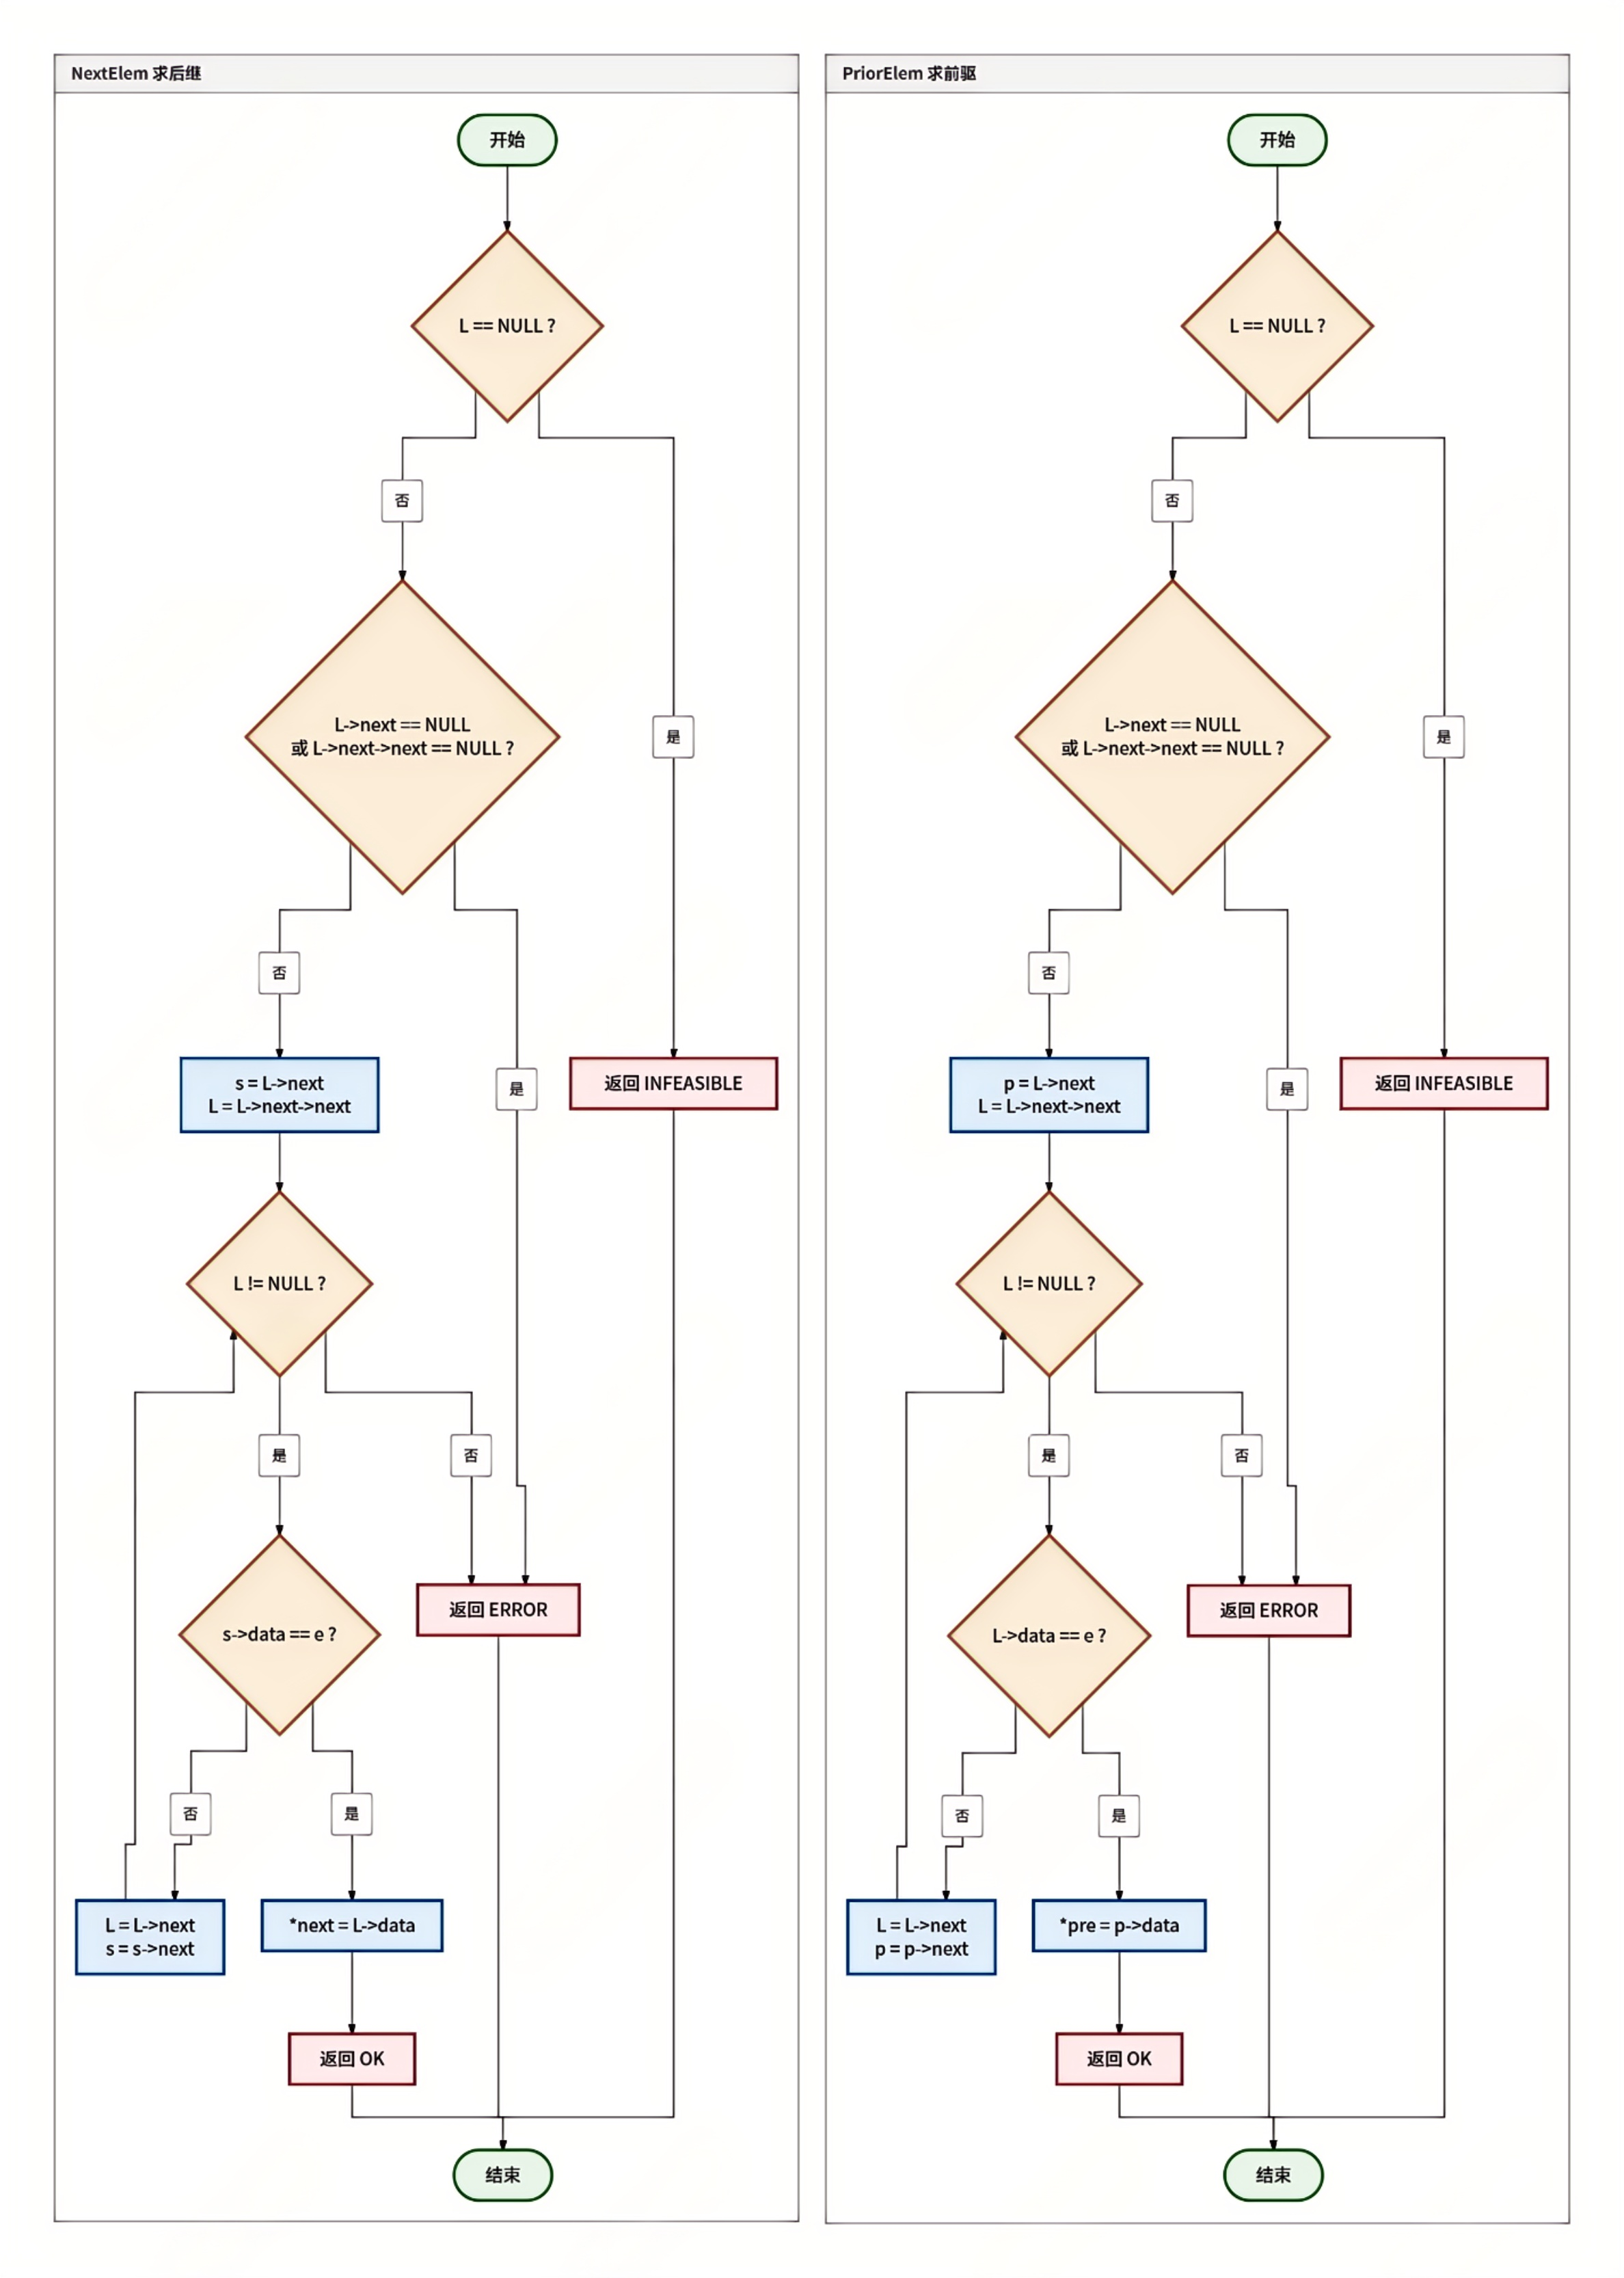
\includegraphics[width=\linewidth]{前驱与后继.png}
	\caption{前驱与后继流程示意}
\end{figure}

\newpage

\subsubsection{ListInsert(L, i, e)——插入元素}
\vspace{-0.8em}
\begin{quote}\small
\textbf{初始条件：}线性表L已存在，$1\leq i\leq\text{ListLength}(L)+1$。\quad\textbf{操作结果：}在L的第i个位置之前插入新的数据元素e。
\end{quote}
\vspace{-0.8em}
{\small 通过双指针p（前驱）、q（当前）定位第$i-1$个节点；新节点t执行\ \texttt{t->next = q; p->next = t}\ 完成搭桥，顺序不可逆。时间复杂度$O(n)$。}

\begin{lstlisting}[label={lst:insert}, caption={ListInsert}, basicstyle=\footnotesize\ttfamily]
status ListInsert(LinkList *L, int i, ElemType e) {
    if (*L == NULL) return INFEASIBLE;
    LinkList p = *L, q = (*L)->next;
    int cnt = 1;
    while (cnt != i && q != NULL) { p = p->next; q = q->next; cnt++; }
    if (cnt != i) return ERROR;
    LinkList t = (LinkList)malloc(sizeof(LNode));
    if (t == NULL) return OVERFLOW;
    t->data = e;  t->next = q;  p->next = t;
    return OK;
}
\end{lstlisting}

\vspace{-2.8em}
\subsubsection{ListDelete(L, i, e)——删除元素}
\vspace{-0.8em}
\begin{quote}\small
\textbf{初始条件：}线性表L已存在且非空，$1\leq i\leq\text{ListLength}(L)$。\quad\textbf{操作结果：}删除L的第i个数据元素并用e返回其值。
\end{quote}
\vspace{-0.8em}
{\small 双指针s（前驱）、f（当前）同步移动，找到目标后执行\ \texttt{*e = f->data; s->next = f->next; free(f)}\ 完成绕行与释放。时间复杂度$O(n)$。}

\begin{lstlisting}[label={lst:delete}, caption={ListDelete}, basicstyle=\footnotesize\ttfamily]
status ListDelete(LinkList *L, int i, ElemType *e) {
    if (*L == NULL) return INFEASIBLE;
    if ((*L)->next == NULL) return ERROR;
    LinkList s = *L, f = (*L)->next;
    int cnt = 1;
    while (f != NULL) {
        if (cnt == i) {
            *e = f->data; s->next = f->next; free(f); return OK;
        }
        f = f->next; s = s->next; cnt++;
    }
    return ERROR;
}
\end{lstlisting}
\newpage
\begin{figure}[!htb]
	\centering
	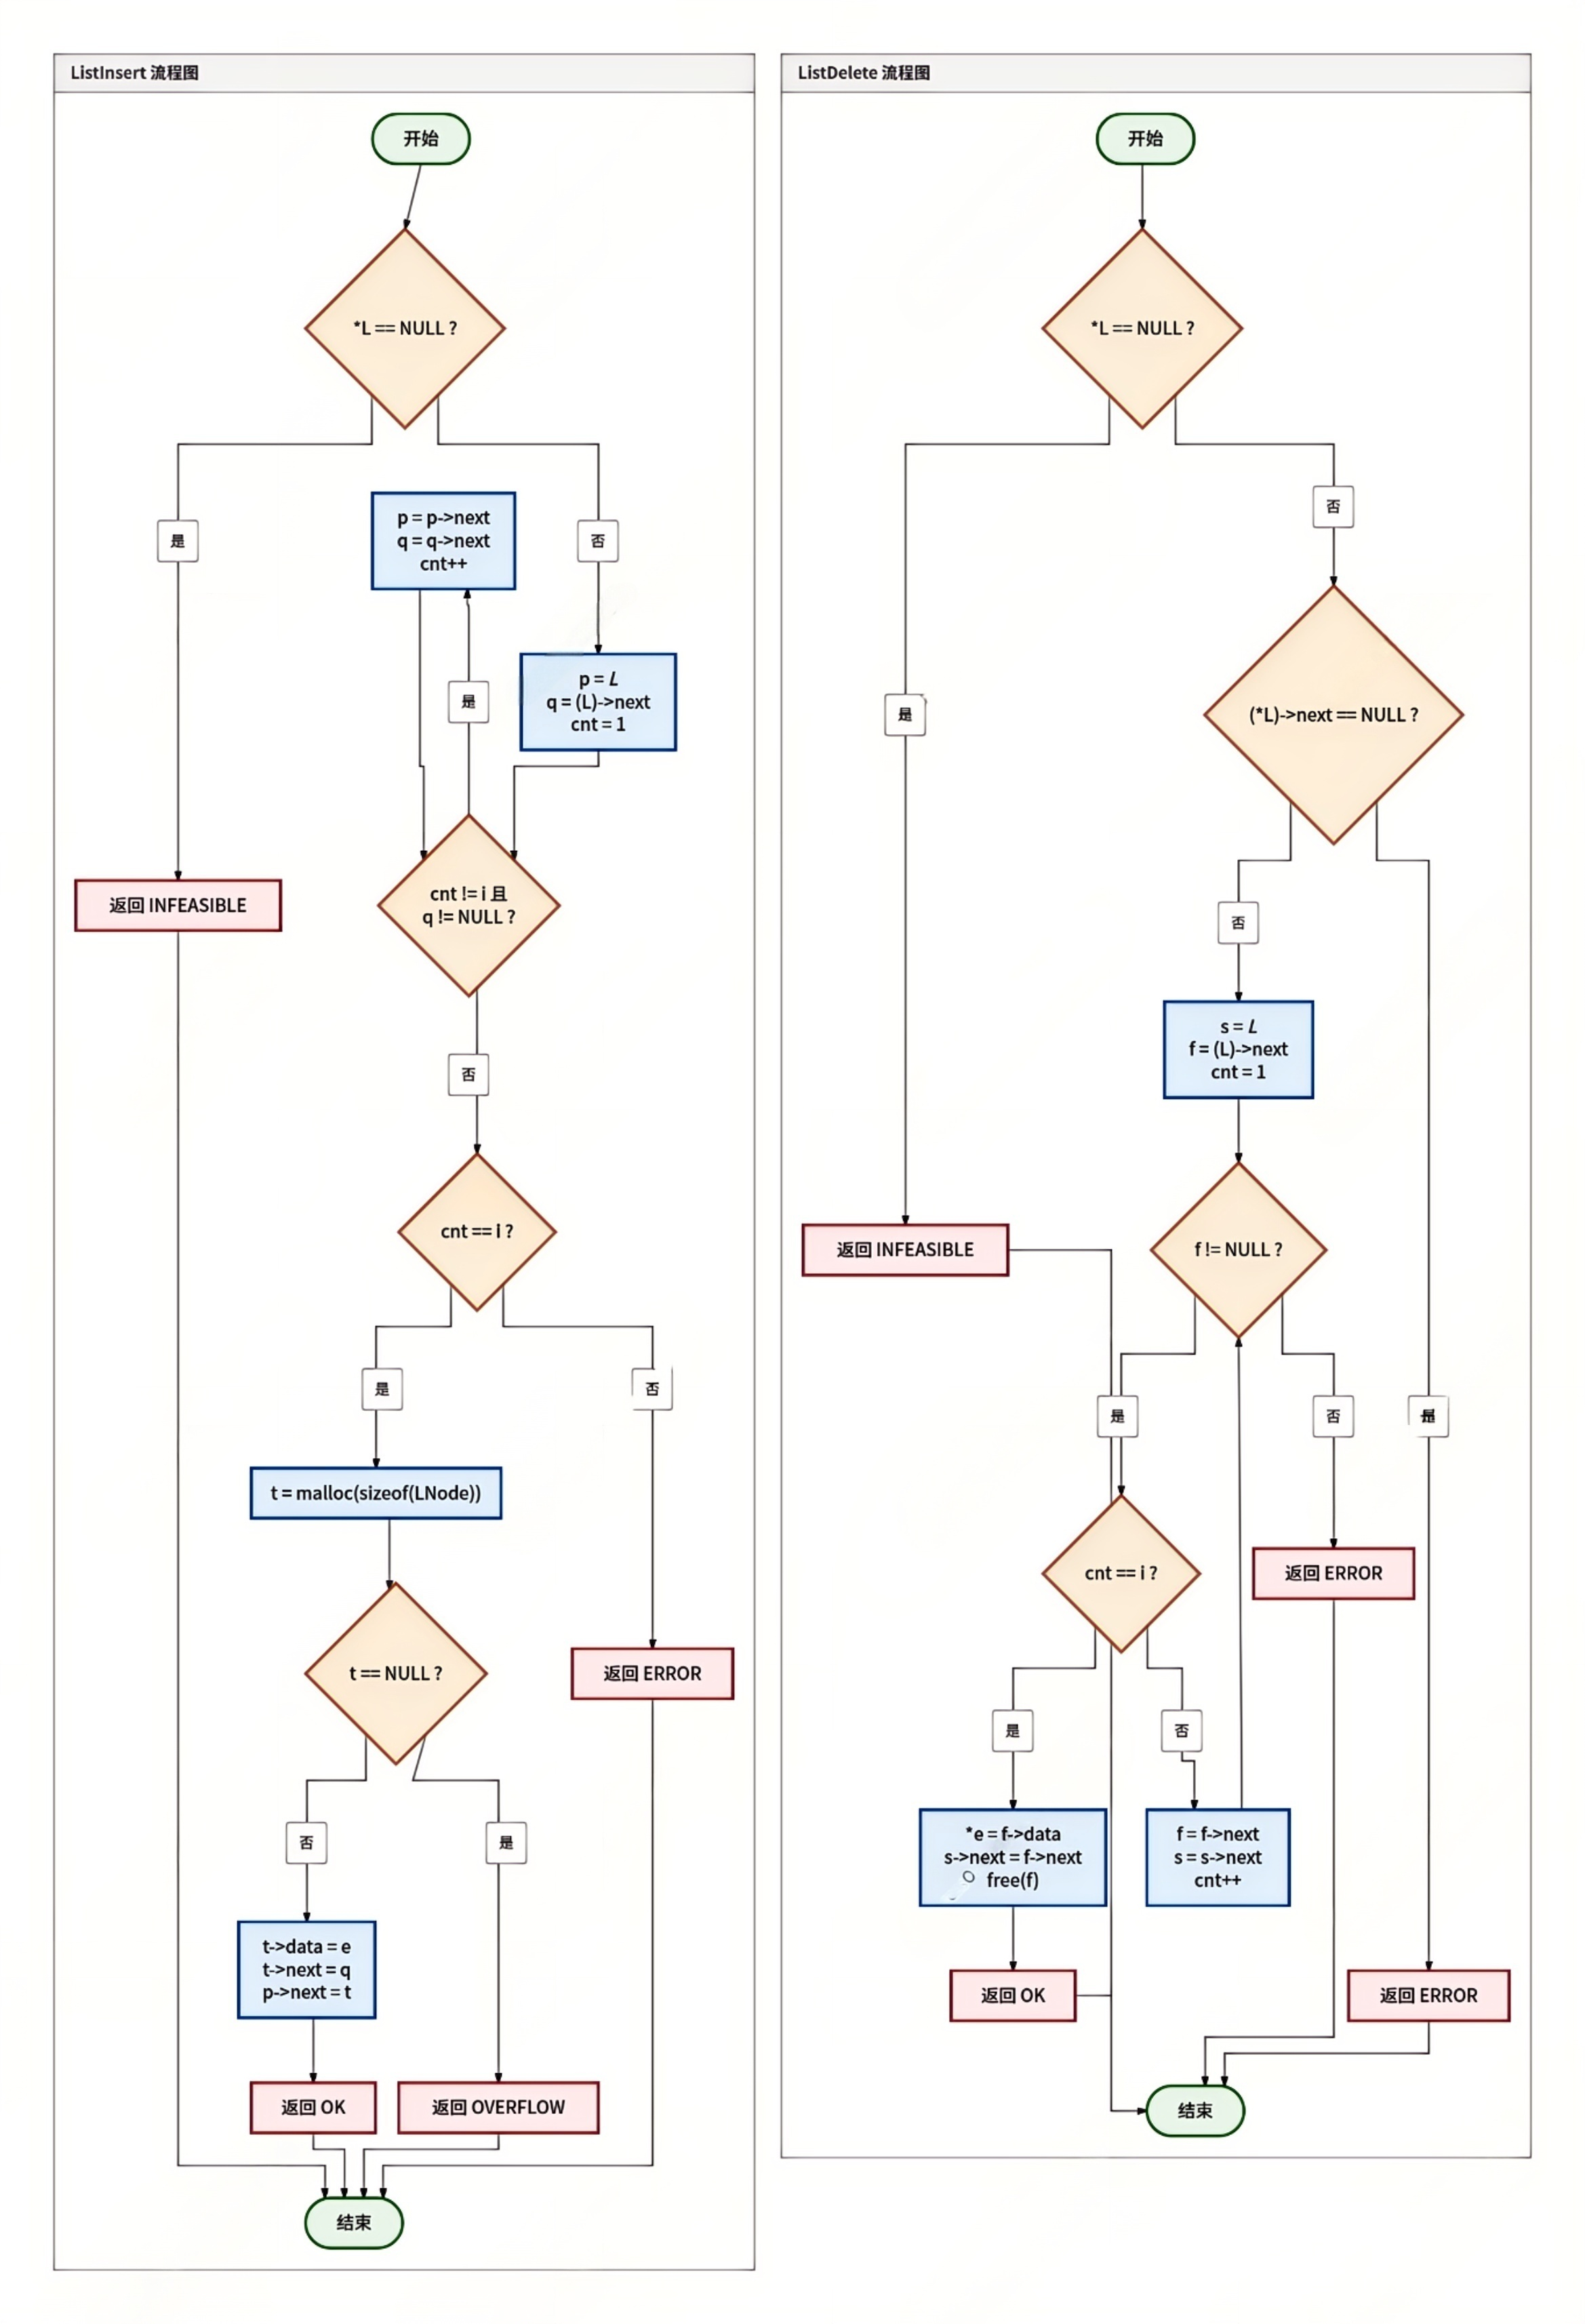
\includegraphics[width=\linewidth]{插入与删除.png}
	\caption{插入与删除}
\end{figure}
\newpage
\subsubsection{ListTraverse(L)——遍历表}
% Mermaid 参考: 图15 (ListTraverse) — 见 Mermaid流程图.txt

\begin{quote}\small
\textbf{初始条件：}线性表L已存在。\quad\textbf{操作结果：}依次输出L的每个数据元素。
\end{quote}

实现分析：从头节点后继开始逐一访问并用黄色(14)高亮输出。仅在非最后元素后加空格避免尾部空白。时间复杂度$O(n)$。

\begin{lstlisting}[label={lst:traverse}, caption={ListTraverse}]
status ListTraverse(LinkList L) {
    if (L == NULL) return INFEASIBLE;
    L = L->next;
    while (L != NULL) {
        SetConsoleColor(14); printf("%d", L->data);
        SetConsoleColor(7);
        if (L->next != NULL) printf(" ");
        L = L->next;
    }
    return OK;
}
\end{lstlisting}

\subsection{附加功能函数分析}

\subsubsection{reverseList(L)——链表翻转}

\begin{quote}\small
\textbf{初始条件：}线性表L已存在。\quad\textbf{操作结果：}将链表L原地逆置。
\end{quote}

\textbf{核心思想：头插法逆置。}将原链表的每个数据节点逐个摘下插入到头节点之后。三个指针联动——p指向当前待处理节点，q保存p的后继，循环执行"保存后继→头插→更新p"。
\vspace{1em}
\begin{figure}[!htb]
	\centering
	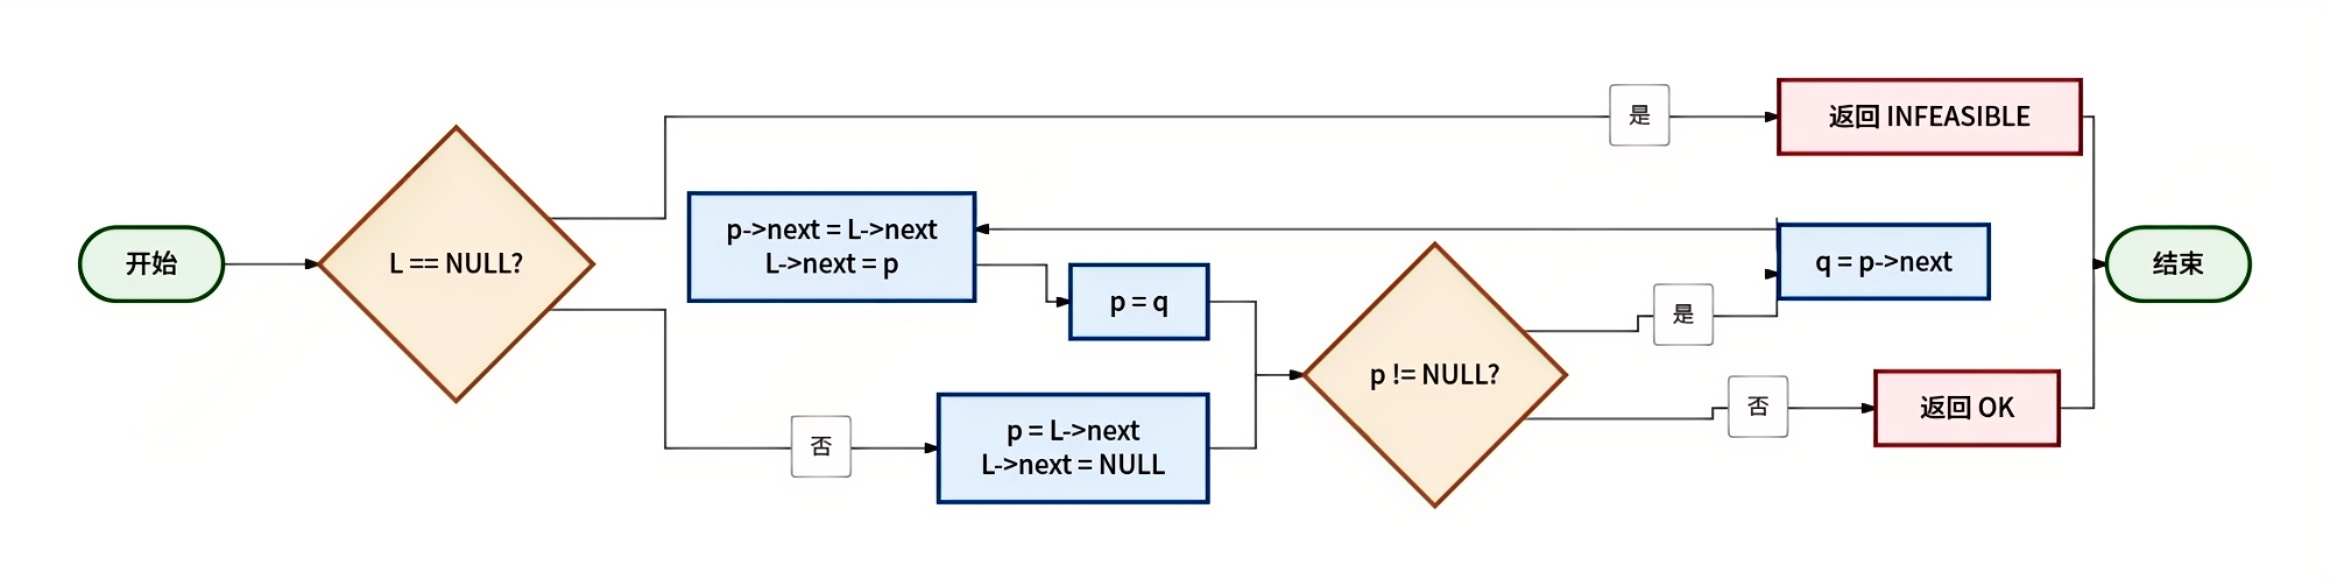
\includegraphics[width=\linewidth]{翻转.png}
	\caption{翻转}
\end{figure}
\newpage
\begin{lstlisting}[label={lst:reverse}, caption={reverseList}]
status reverseList(LinkList L) {
    if (L == NULL) return INFEASIBLE;
    LinkList p = L->next;
    L->next = NULL;
    while (p != NULL) {
        LinkList q = p->next;
        p->next = L->next;
        L->next = p;
        p = q;
    }
    return OK;
}
\end{lstlisting}

\textbf{算法分析：}原地逆置，仅用三个指针，空间$O(1)$、时间$O(n)$。循环体内四行顺序绝对不可调换——必须先保存q再修改p->next。过程示例：初始L→1→2→3→NULL：$(1)$p=1→L→NULL；$(2)$q=2,头插1→L→1→NULL；$(3)$q=3,头插2→L→2→1→NULL；$(4)$q=NULL,头插3→L→3→2→1→NULL。

\subsubsection{RemoveNthFromEnd(L, n)——删除倒数第N个节点}
% Mermaid 参考: 图17 (RemoveNthFromEnd) — 见 Mermaid流程图.txt

\begin{quote}\small
\textbf{初始条件：}线性表L已存在且非空。\quad\textbf{操作结果：}删除链表倒数第n个节点。
\end{quote}

\textbf{核心思想：快慢指针法。}fast先走n步，然后fast和slow同步前进。当fast抵达NULL时，slow恰好指向倒数第n个节点的前驱。

\begin{figure}[htb]
	\centering
	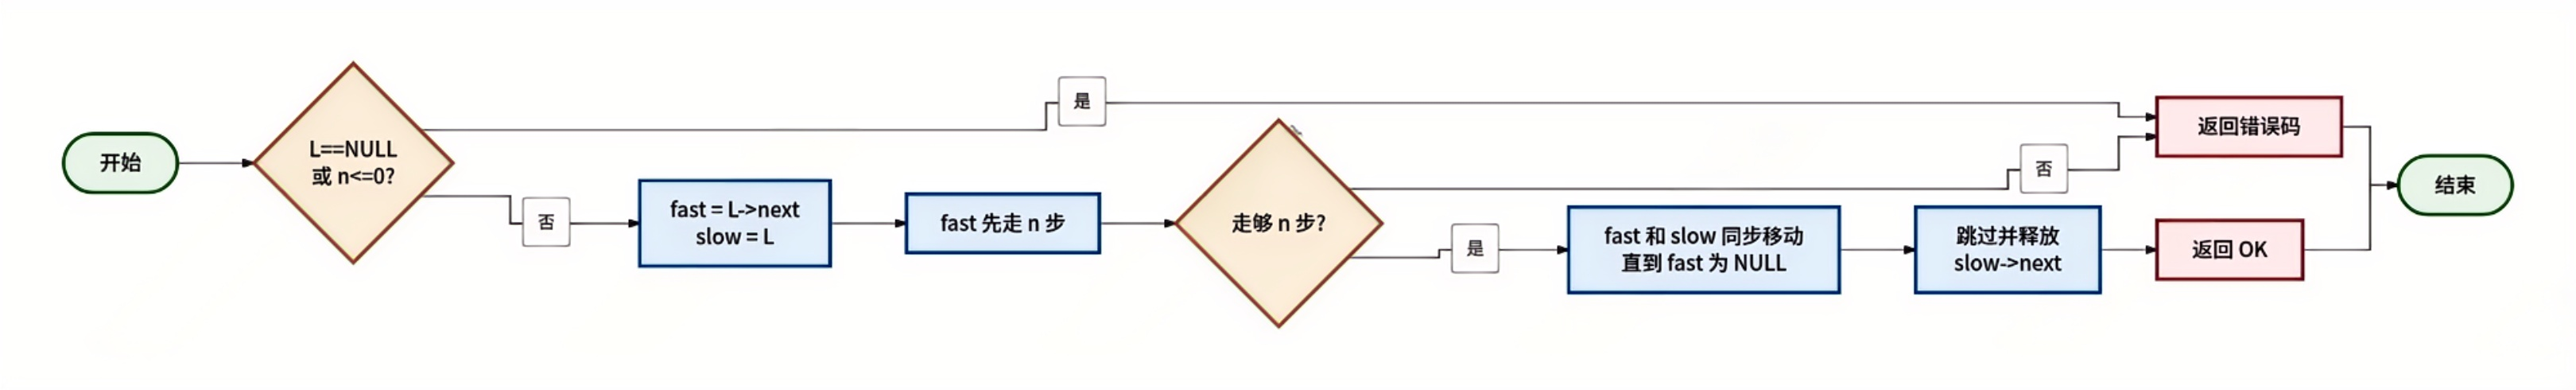
\includegraphics[width=\linewidth]{删除倒数第n个 (3).png}
	\caption{删除倒数第N个}
\end{figure}

% Mermaid 参考: 图17 (RemoveNthFromEnd 快慢指针法) — 见 Mermaid流程图.txt
\begin{lstlisting}[label={lst:removenth}, caption={RemoveNthFromEnd}]
status RemoveNthFromEnd(LinkList L, int n) {
    if (L == NULL) return INFEASIBLE;
    if (n <= 0) return ERROR;
    LinkList fast = L->next, slow = L;
    int i;
    for (i = 0; i < n && fast != NULL; i++) fast = fast->next;
    if (i < n) return ERROR;
    while (fast != NULL) { slow = slow->next; fast = fast->next; }
    LinkList del = slow->next;
    slow->next = del->next; free(del);
    return OK;
}
\end{lstlisting}

\textbf{精巧之处：}slow从\textbf{头节点}开始（而非第一个数据节点），确保fast到NULL时slow恰好是前驱。时间$O(n)$、空间$O(1)$，仅需一次遍历。

\subsubsection{sortList(L)——链表排序}
% Mermaid 参考: 图18 (sortList 冒泡排序) — 见 Mermaid流程图.txt

\begin{quote}\small
\textbf{初始条件：}线性表L已存在。\quad\textbf{操作结果：}将L中的数据元素按升序排列。
\end{quote}

实现分析：采用冒泡排序，通过交换节点\textbf{数据域}（\texttt{tmp = q->data; q->data = p->data; p->data = tmp}）实现排序，避免了复杂的指针域交换。时间复杂度$O(n^2)$，空间$O(1)$。改进方向：可引入归并排序（$O(n\log n)$）或增加swapped标志提前退出。
\begin{figure}[htb]
	\centering
	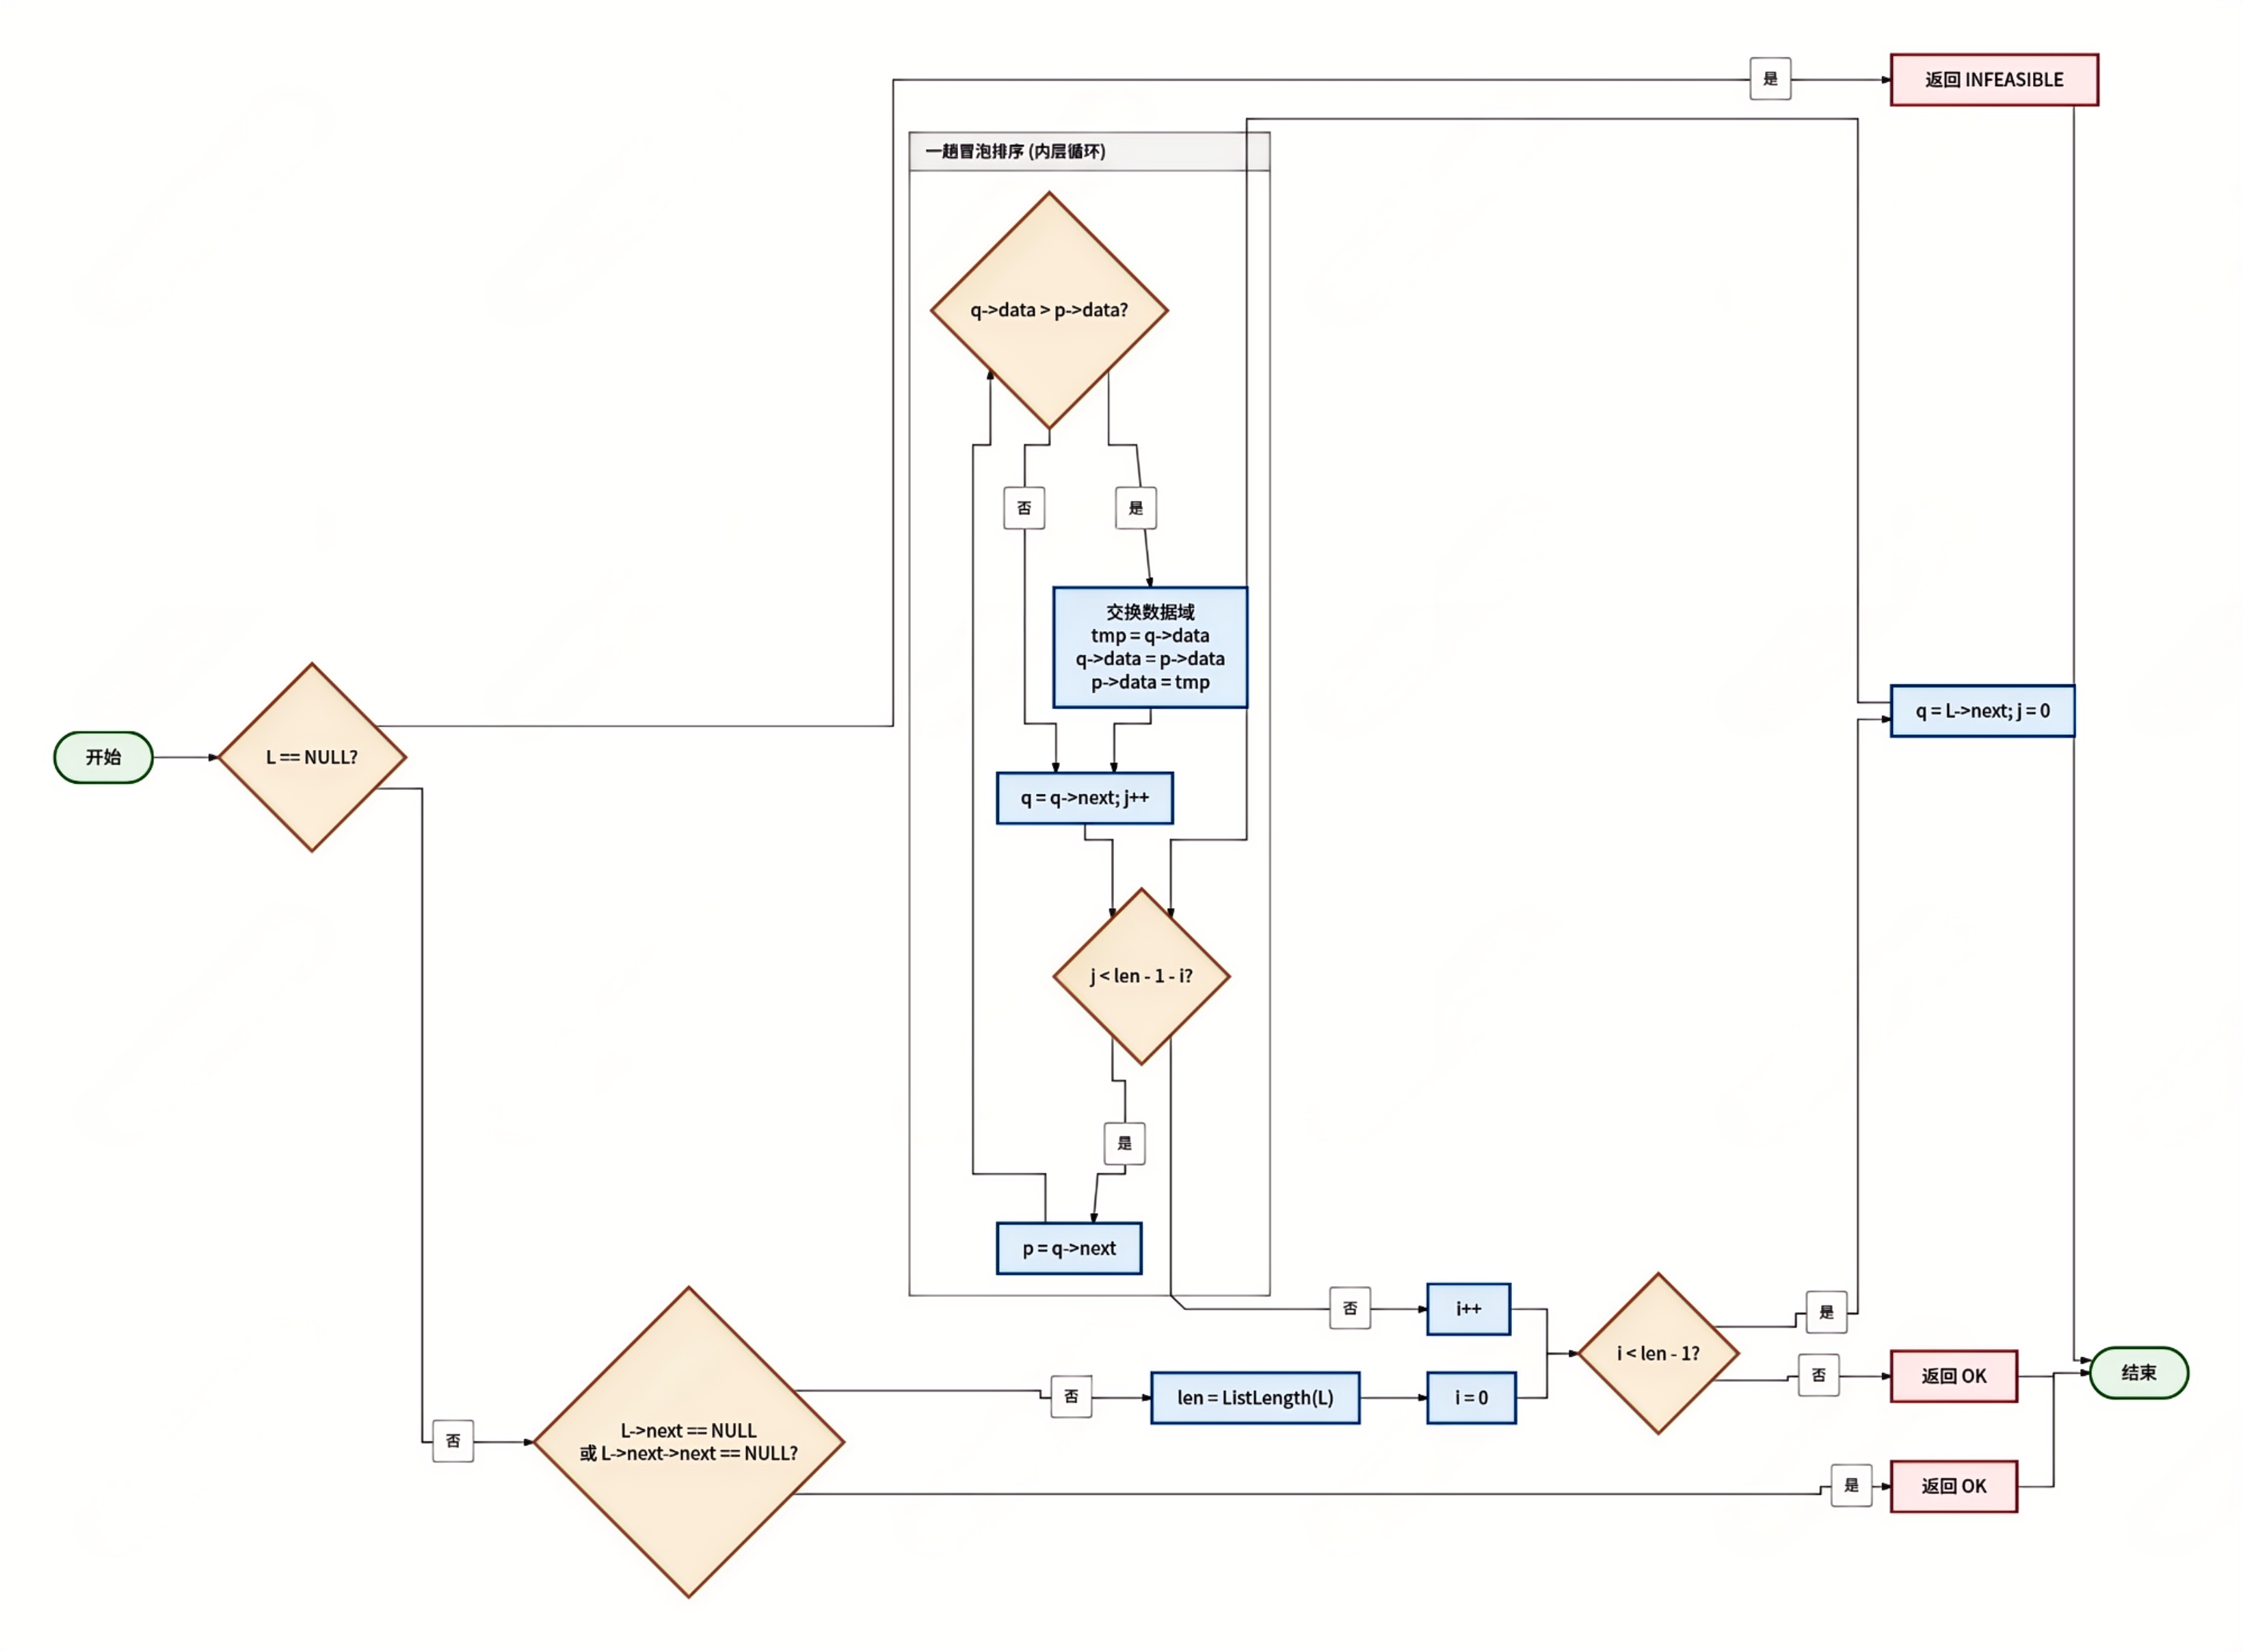
\includegraphics[width=\linewidth]{排序2.png}
	\caption{排序}
\end{figure}
\begin{lstlisting}[label={lst:sort}, caption={sortList}]
status sortList(LinkList L) {
    if (L == NULL) return INFEASIBLE;
    if (L->next == NULL || L->next->next == NULL) return OK;
    int len = ListLength(L);
    for (int i = 0; i < len - 1; i++) {
        LinkList q = L->next;
        for (int j = 0; j < len - 1 - i; j++) {
            LinkList p = q->next;
            if (q->data > p->data) {
                ElemType tmp = q->data;
                q->data = p->data; p->data = tmp;
            }
            q = q->next;
        }
    }
    return OK;
}
\end{lstlisting}

\subsubsection{文件形式保存与加载}

% Mermaid 参考: 图19 (SaveList), 图20 (LoadList) — 见 Mermaid流程图.txt
\begin{quote}\small
\textbf{操作结果：}设计文件数据记录格式保存链表逻辑结构(D,\{R\})，支持从空表加载文件生成单链表。
\end{quote}

\textbf{SaveList：}以空格分隔的文本格式顺序写入数据元素。\textbf{LoadList：}尾插法重建链表——维护tail指针始终指向尾节点，新节点追加到tail之后，确保元素顺序与文件一致。若已有旧链表先DestroyList。文件格式为纯文本，一行或多行空格分隔的整数。

\begin{figure}[htb]
	\centering
	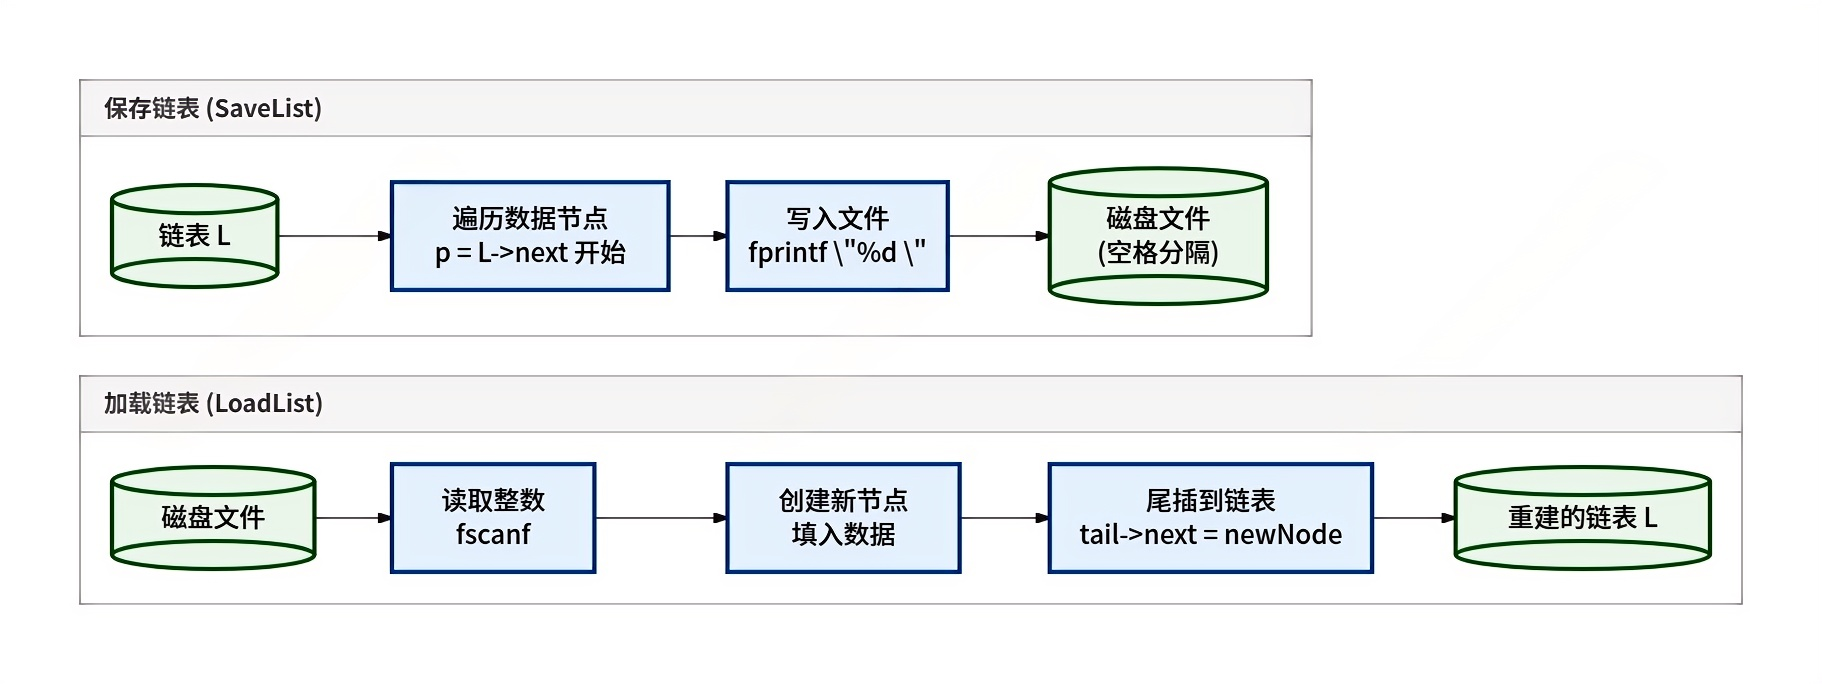
\includegraphics[width=\linewidth]{文件.png}
	\caption{文件存取}
\end{figure}

\begin{lstlisting}[label={lst:file}, caption={SaveList与LoadList}]
status SaveList(LinkList L, char FileName[]) {
    if (L == NULL) return INFEASIBLE;
    FILE *fp = fopen(FileName, "w");
    if (fp == NULL) return ERROR;
    LinkList p = L->next;
    while (p != NULL) { fprintf(fp, "%d ", p->data); p = p->next; }
    fclose(fp); return OK;
}
status LoadList(LinkList *L, char FileName[]) {
    if (*L != NULL) DestroyList(L);
    FILE *fp = fopen(FileName, "r");
    if (fp == NULL) return ERROR;
    *L = (LinkList)malloc(sizeof(LNode));
    if (*L == NULL) { fclose(fp); return OVERFLOW; }
    (*L)->next = NULL;
    LinkList tail = *L; int data;
    while (fscanf(fp, "%d", &data) != EOF) {
        LinkList newNode = (LinkList)malloc(sizeof(LNode));
        if (newNode == NULL) { fclose(fp); return OVERFLOW; }
        newNode->data = data; newNode->next = NULL;
        tail->next = newNode; tail = newNode;
    }
    fclose(fp); return OK;
}
\end{lstlisting}

\subsection{多表管理功能分析}

\subsubsection{数据结构设计}

实验要求"实现多个线性表管理：设计相应的数据结构管理多个线性表的查找、添加、移除等功能"。系统采用\texttt{LISTS}结构体作为容器，将多个\texttt{NamedList}组织在固定容量的数组中，通过\texttt{length}字段记录有效元素个数，通过\texttt{currentIdx}（在\texttt{multiTableMode}函数内部维护）记录当前选中的元素下标。

\texttt{LISTS}结构体设计如下：
\begin{itemize}
    \item \texttt{NamedList elem[MAX\_LIST\_NUM]}——固定容量的命名线性表数组（容量10），每个NamedList含\texttt{char name[20]}（唯一的名称标识符）和\texttt{LinkList L}（指向单链表头节点的指针）
    \item \texttt{int length}——当前实际存储的命名线性表数量，同时作为下次追加的位置索引
\end{itemize}

内存布局方面，LISTS结构体占据一块连续内存（约\texttt{sizeof(NamedList)×10+sizeof(int)}字节），前\texttt{length}个元素存储有效数据，后续槽位为空闲。每个NamedList内部，L指针要么为NULL（表示链表尚未初始化），要么指向堆上通过InitList分配的单链表。LISTS本身不拥有链表的内存，仅持有指针引用，链表的实际生命周期仍由InitList/DestroyList管理。

\begin{figure}[!htb]
\centering\footnotesize
\resizebox{\textwidth}{!}{
\begin{tikzpicture}[
    box/.style={rectangle, minimum width=3.0cm, minimum height=0.55cm, align=center, draw=black, font=\tiny},
    sbox/.style={rectangle, minimum width=2.2cm, minimum height=0.45cm, align=center, draw=black, fill=blue!8, font=\tiny},
    arrow/.style={thick,->,>=Stealth}
]
\draw [thick, fill=gray!5] (0,0) rectangle (14,-4.2);
\node [font=\footnotesize\bfseries] at (7,0.3) {LISTS 内存区域};
\draw [thick, fill=green!10] (0.2,-0.4) rectangle (6.5,-1.6);
\node [font=\tiny] at (3.35,-0.2) {elem[0] (NamedList)};
\node [font=\tiny] at (3.35,-0.7) {name = "ListA"};
\node [font=\tiny] at (3.35,-1.1) {L = 0x1A2B (指向头节点)};
\draw [thick, fill=green!10] (0.2,-1.7) rectangle (6.5,-2.9);
\node [font=\tiny] at (3.35,-1.5) {elem[1] (NamedList)};
\node [font=\tiny] at (3.35,-2.0) {name = "ListB"};
\node [font=\tiny] at (3.35,-2.4) {L = NULL (未初始化)};
\draw [thick, fill=green!10] (0.2,-3.0) rectangle (6.5,-4.0);
\node [font=\tiny] at (3.35,-2.8) {elem[2] (NamedList)};
\node [font=\tiny] at (3.35,-3.3) {name = "MyData"};
\node [font=\tiny] at (3.35,-3.7) {L = 0x3F8C (指向头节点)};
\draw [thick, fill=yellow!15] (7.0,-0.4) rectangle (13.8,-1.2);
\node [font=\tiny] at (10.4,-0.6) {length = 3};
\node [font=\tiny] at (10.4,-1.0) {(elem[0..2]有效)};
\node (l0) [sbox, right=1.0cm of {6.5,-0.8}, fill=yellow!12] {Head→5→3→NULL};
\draw [arrow, dashed] (4.5,-1.1) -- (l0.west);
\node (l2) [sbox, right=1.0cm of {6.5,-3.3}, fill=yellow!12] {Head→8→2→NULL};
\draw [arrow, dashed] (4.5,-3.7) -- (l2.west);
\end{tikzpicture}
}
\caption{LISTS内存布局示意图（length=3，其中elem[1]的链表尚未初始化）}
\label{fig:lists-memory}
\end{figure}

\subsubsection{AddList——添加线性表}
% Mermaid 参考: 图21 (AddList) — 见 Mermaid流程图.txt
% Mermaid 参考: 图2 (LISTS内存布局) — 见 Mermaid流程图.txt

\texttt{AddList(LISTS *Lists, char ListName[])}在LISTS数组尾部追加一个新的命名线性表条目。初始条件是LISTS容量未满（\texttt{length < MAX\_LIST\_NUM}），操作结果是在elem[length]位置创建新条目并递增length。

函数首先检查容量边界（\texttt{length >= MAX\_LIST\_NUM}时返回ERROR）；然后逐字符复制名称字符串并添加终止符\texttt{\textbackslash0}；接着将链表指针L显式置为NULL；最后\texttt{length++}。

值得注意的设计决策是：AddList仅创建命名槽位，不调用InitList初始化链表。原因是InitList需要\texttt{malloc}分配头节点，属于资源获取操作。推迟到用户进入单表菜单手动选择"初始化"时执行，给予用户完整的操作控制权。

\begin{lstlisting}[caption={AddList函数}]
status AddList(LISTS *Lists, char ListName[]) {
    if (Lists->length >= MAX_LIST_NUM) return ERROR;
    int i = 0;
    while (ListName[i]) {
        Lists->elem[Lists->length].name[i] = ListName[i];
        i++;
    }
    Lists->elem[Lists->length].name[i] = '\0';
    Lists->elem[Lists->length].L = NULL;
    Lists->length++;
    return OK;
}
\end{lstlisting}

\subsubsection{RemoveList——删除线性表}
% Mermaid 参考: 图22 (RemoveList) — 见 Mermaid流程图.txt

\texttt{RemoveList(LISTS *Lists, char ListName[])}按名称查找并删除指定的命名线性表。初始条件是LISTS中存在与ListName匹配的条目，操作结果是销毁该条目持有的链表并移除条目本身。

函数分三步执行：

\begin{enumerate}
    \item \textbf{线性搜索}：遍历elem数组，用\texttt{strcmp}比较名称，找到匹配元素的下标pos。若未找到返回ERROR。
    \item \textbf{释放链表资源}：调用\texttt{DestroyList(\&Lists->elem[pos].L)}释放该元素持有的全部LNode节点内存。
    \item \textbf{数组前移}：将pos之后的所有元素前移一位，填补被删位置的空洞，然后\texttt{length--}。
\end{enumerate}

步骤2和步骤3的顺序至关重要。若先执行数组前移，被删元素的链表指针将被覆盖而丢失，造成永久内存泄漏。正确顺序必须是"先释放资源，再移动数组"。

\begin{lstlisting}[caption={RemoveList函数}]
status RemoveList(LISTS *Lists, char ListName[]) {
    int pos = -1;
    for (int i = 0; i < Lists->length; i++)
        if (strcmp(Lists->elem[i].name, ListName) == 0)
            { pos = i; break; }
    if (pos == -1) return ERROR;
    DestroyList(&Lists->elem[pos].L);
    for (int i = pos; i < Lists->length - 1; i++)
        Lists->elem[i] = Lists->elem[i + 1];
    Lists->length--;
    return OK;
}
\end{lstlisting}

\subsubsection{LocateList与ListAllNames}
% Mermaid 参考: 图23 (LocateList) — 见 Mermaid流程图.txt

\texttt{LocateList(LISTS Lists, char ListName[])}顺序扫描elem数组，返回匹配名称的元素序号（从1开始），未找到返回0。返回1-based序号而非0-based下标的设计，使得0可直接作为布尔判断的"假"值，简化调用者代码。

\texttt{ListAllNames(LISTS Lists)}为辅助显示函数，遍历所有命名线性表并以彩色格式输出序号、名称和链表长度。其中名称使用绿色(颜色码10)突出显示，长度为辅助信息的青色(颜色码11)。

\begin{lstlisting}[caption={LocateList与ListAllNames}]
% Mermaid 参考: 图23 (LocateList) — 见 Mermaid流程图.txt
int LocateList(LISTS Lists, char ListName[]) {
    for (int i = 0; i < Lists.length; i++)
        if (strcmp(Lists.elem[i].name, ListName) == 0)
            return i + 1;
    return 0;
}
void ListAllNames(LISTS Lists) {
    SetConsoleColor(3);
    printf("\n当前线性表列表 (%d个):\n", Lists.length);
    SetConsoleColor(7);
    for (int i = 0; i < Lists.length; i++) {
        printf("  [%d] ", i + 1);
        SetConsoleColor(10); printf("%s", Lists.elem[i].name);
        SetConsoleColor(7);
        printf(" (长度:");
        SetConsoleColor(11); printf("%d", ListLength(Lists.elem[i].L));
        SetConsoleColor(7); printf(")\n");
    }
}
\end{lstlisting}

\subsubsection{multiTableMode——交互控制逻辑}
% Mermaid 参考: 图24 (multiTableMode 状态转换) — 见 Mermaid流程图.txt

\texttt{multiTableMode()}是多表管理模式的入口函数。其内部维护一个\texttt{currentIdx}变量（初始为-1，表示未选中任何表），通过一个无限循环显示顶层菜单并处理五种用户操作：

\begin{enumerate}
    \item \textbf{新建表（case 1）}：读取表名，调用\texttt{AddList(\&lists, name)}追加。由于AddList不自动初始化链表，新建后的表处于"条目存在但链表未就绪"状态。
    \item \textbf{选择表（case 2）}：读取表名，调用\texttt{LocateList(lists, name)}查找。若找到则设置\texttt{currentIdx = idx - 1}（从1-based序号转回0-based下标），后续对"当前表"的引用通过\texttt{\&lists.elem[currentIdx].L}定位。
    \item \textbf{删除表（case 3）}：读取表名，调用\texttt{RemoveList(\&lists, name)}。若被删表恰好是当前选中的表，需要将\texttt{currentIdx}重置为-1，防止后续操作访问已释放的内存。
    \item \textbf{操作当前表（case 4）}：首先检查\texttt{currentIdx != -1}，然后调用\\
    \texttt{operateTableMenu(\&lists.elem[currentIdx].L)}进入单表操作菜单。此处传递的是二级指针，使得单表菜单内可以修改链表头指针本身。
    \item \textbf{返回上级（case 5）}：退出multiTableMode，回到main函数的主菜单。
\end{enumerate}

\begin{figure}[htb]
	\centering
	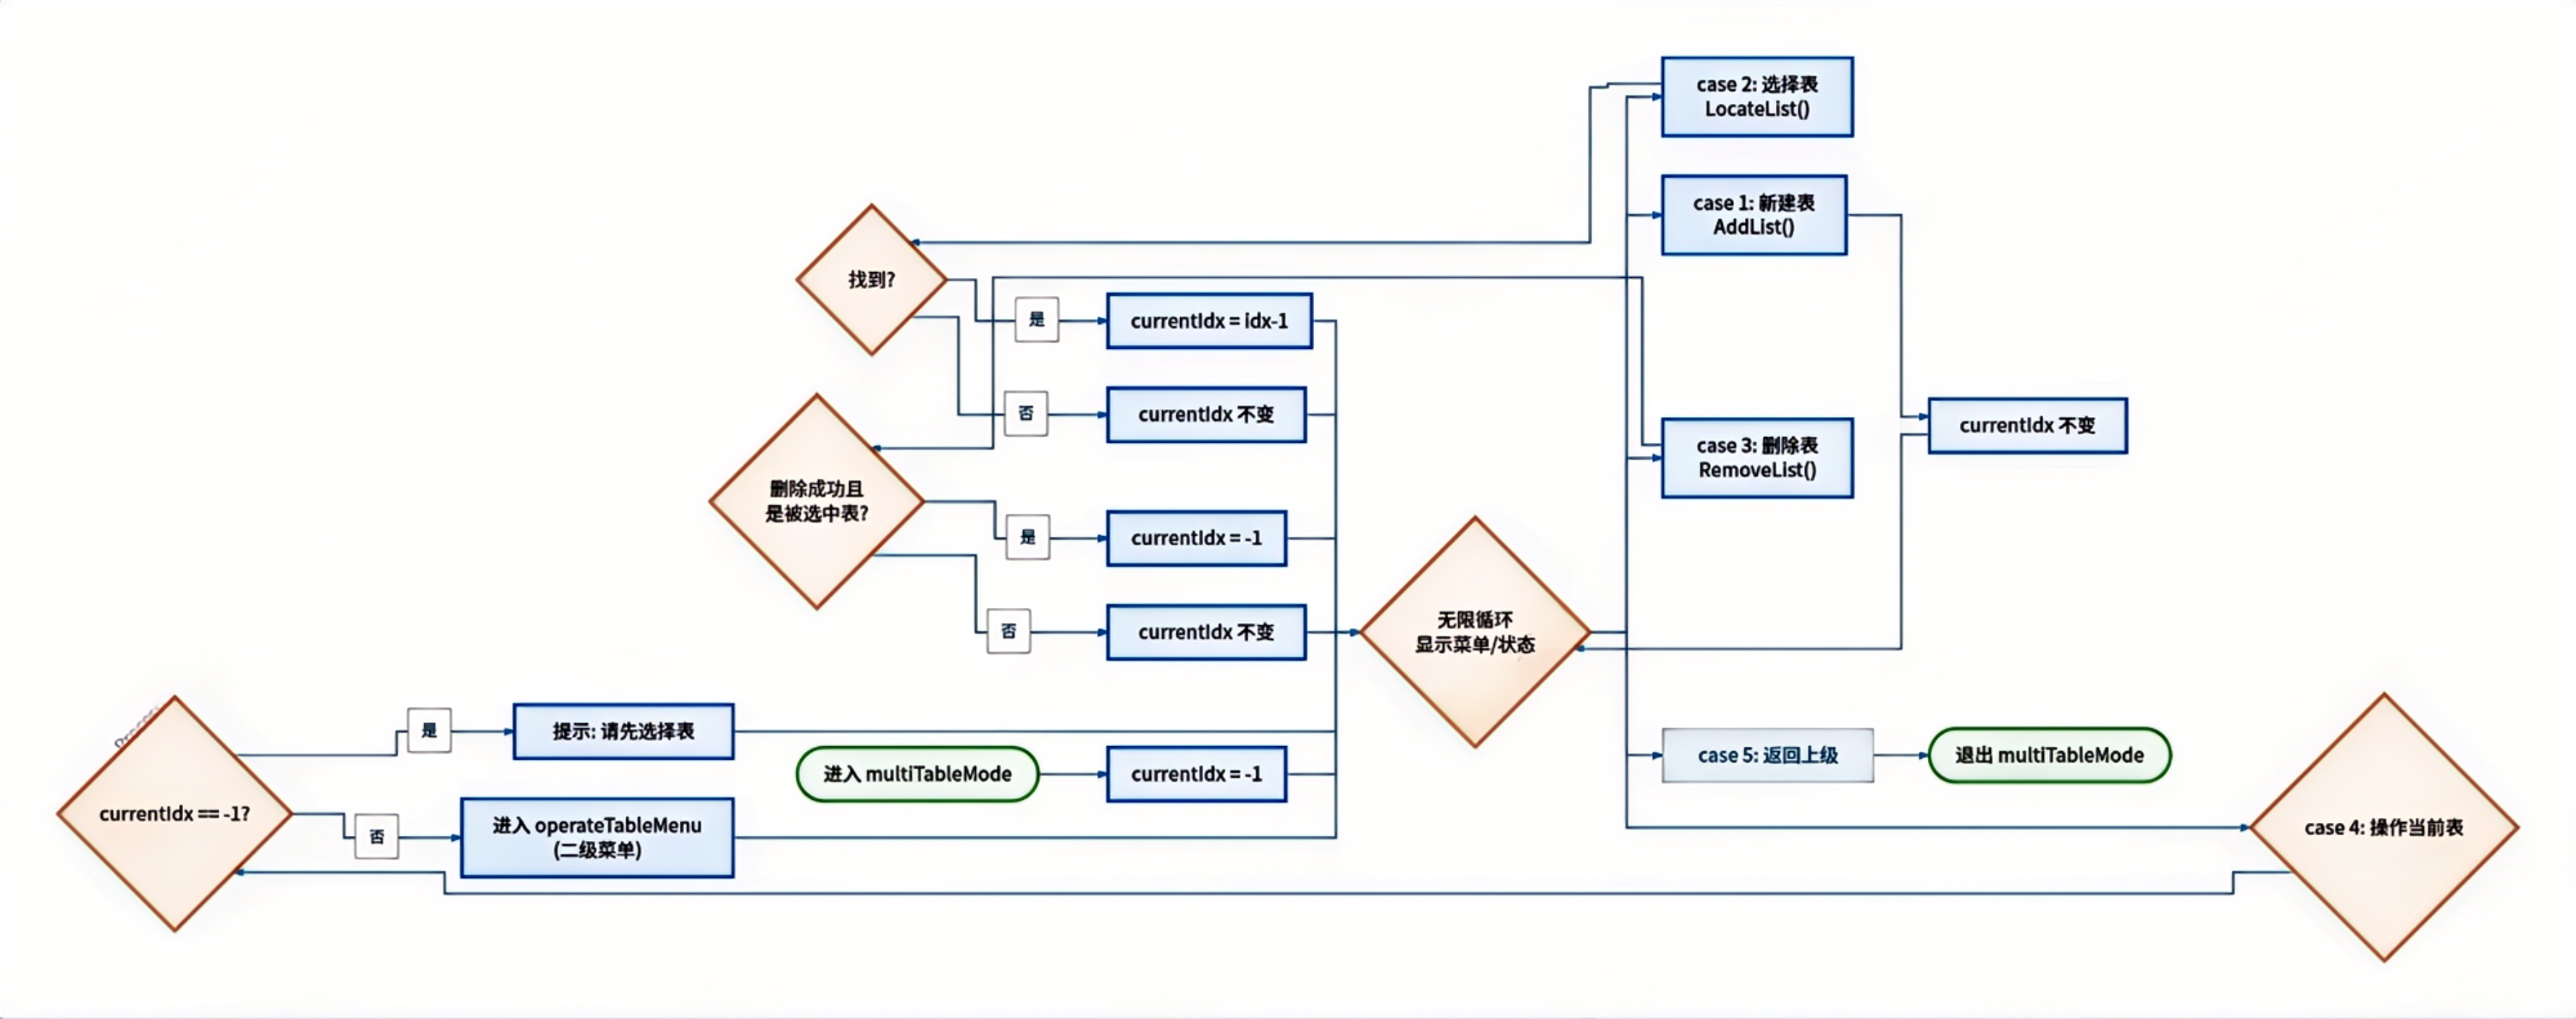
\includegraphics[width=\linewidth]{交互.png}
	\caption{交互}
\end{figure}

% Mermaid 参考: 图24 (multiTableMode 状态转换) — 见 Mermaid流程图.txt
\subsubsection{全局变量与模块耦合}

系统将唯一的 \texttt{LISTS} 实例 \texttt{lists} 声明为文件作用域的全局变量，所有多表管理函数和交互函数均直接访问该全局量。这避免了在函数间层层传递指针，使调用接口更加简洁；代价是模块间存在隐式耦合——任何函数都可能修改 \texttt{lists}，调试时需要留意修改来源。


\textbf{模块访问方式与耦合特征：}
\begin{itemize}
    \item \texttt{AddList} 仅在数组尾部追加一个“表条目”，并将 \texttt{L} 置为 \texttt{NULL}（不自动初始化链表），随后递增 \texttt{length}。
    \item \texttt{RemoveList} 按名称删除条目，先调用 \texttt{DestroyList} 释放链表，再移动后续元素并递减 \texttt{length}。这里必须“先释放、再移动”，否则被覆盖的 \texttt{L} 指针将造成内存泄漏。
    \item \texttt{LocateList} 线性搜索后返回 1‑based 序号（0 表示不存在），方便上层用 \texttt{if(idx)} 判断。
    \item \texttt{ListAllNames} 遍历有效条目，显示表名与长度，只读访问不修改全局状态。
\end{itemize}
所有函数都直接读写 \texttt{lists}，形成以全局变量为中心的“辐射状”依赖关系。这种设计在小型系统中足够清晰，但若扩展到更多模块，建议封装为单例或通过参数显式传递。

\textbf{数据流与依赖关系：}
下图展示了顶层调用关系以及全局变量 \texttt{lists} 的共享路径。



\begin{figure}[htb]
	\centering
	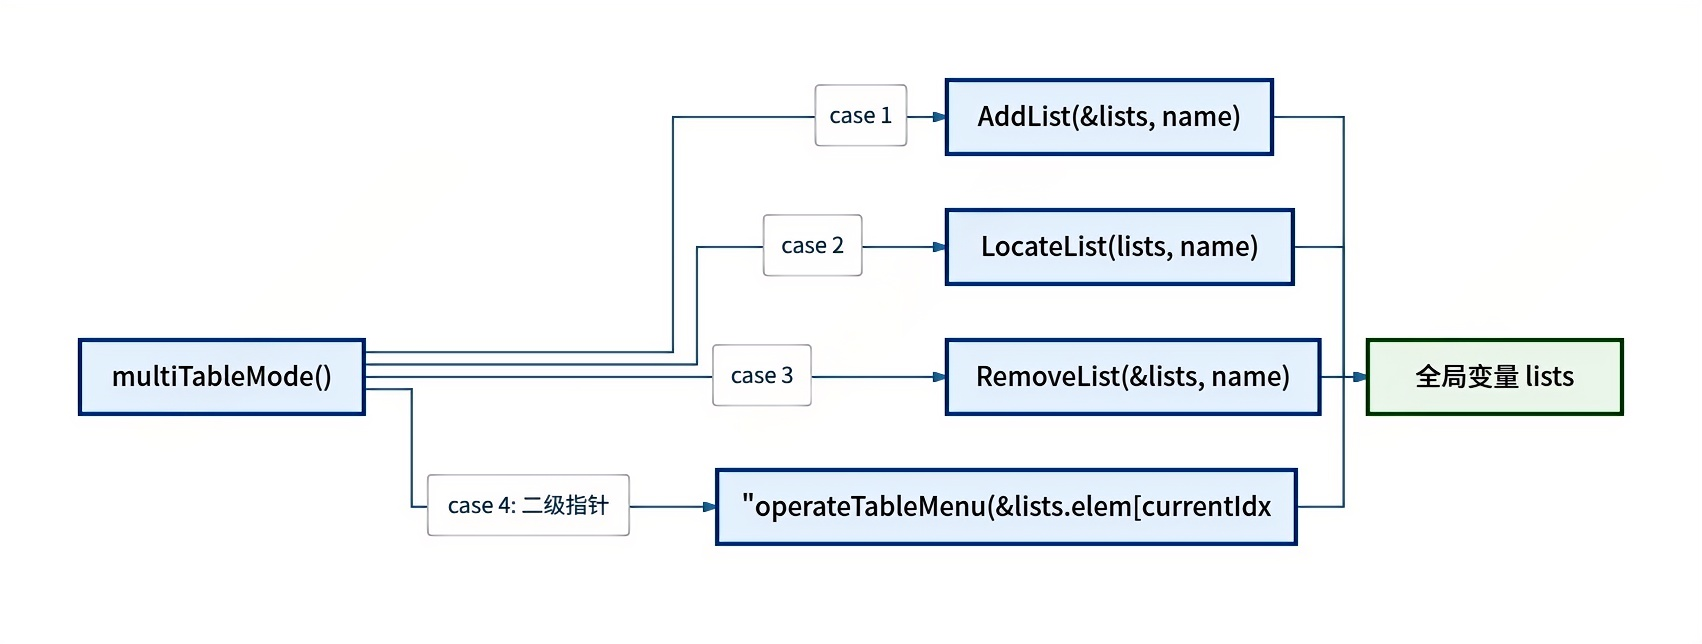
\includegraphics[width=\linewidth]{多表.png}
	\caption{多表管理模块之间的逻辑关系}
\end{figure}

\textbf{设计权衡与模式总结：}
全局变量 \texttt{lists} 的引入使多表管理函数的接口保持简洁（例如 \texttt{AddList} 只需要表名，无需传递容器指针），但模块间的耦合变为隐式的——修改 \texttt{lists} 的函数散落在不同位置，排查问题需要检查所有引用点。  
从抽象层面看，\texttt{LISTS} 实现了一种“名称→资源句柄”的元数据容器模式：用户通过名称选择表，再由句柄（\texttt{LinkList} 指针）访问具体链表。这种模式与操作系统的文件描述符表、数据库的目录表类似，都是将符号名映射到实际资源，实现了**资源访问的间接性**。在程序规模较小时，全局变量带来的便利通常超过其风险；若系统进一步扩展，可考虑将 \texttt{lists} 封装为静态全局变量并提供访问接口，以控制修改入口。
\newpage

\subsection{算法复杂度汇总}

\begin{table}[H]\centering
\caption{线性表各操作算法复杂度}
\label{tbl:complexity1}\renewcommand\arraystretch{1.2}
\begin{tabular}{|c|c|c|c|}\hline
\textbf{操作} & \textbf{函数} & \textbf{时间} & \textbf{空间} \\\hline
初始化 & InitList & $O(1)$ & $O(1)$ \\\hline
销毁/清空 & DestroyList/ClearList & $O(n)$ & $O(1)$ \\\hline
判空 & ListEmpty & $O(1)$ & $O(1)$ \\\hline
求长/取值/查找/前驱/后继 & ListLength/GetElem/LocateElem/Prior/Next & $O(n)$ & $O(1)$ \\\hline
插入/删除 & ListInsert/ListDelete & $O(n)$ & $O(1)$ \\\hline
遍历 & ListTraverse & $O(n)$ & $O(1)$ \\\hline
逆置 & reverseList & $O(n)$ & $O(1)$ \\\hline
删除倒数N & RemoveNthFromEnd & $O(n)$ & $O(1)$ \\\hline
排序 & sortList & $O(n^2)$ & $O(1)$ \\\hline
文件读写 & SaveList/LoadList & $O(n)$ & $O(1)$ \\\hline
\end{tabular}
\end{table}
\vspace{0.5em}
{\small
从表 \ref{tbl:complexity1} 可以归纳出线性表链式存储的几项总体特征：

\textbf{1. 基本操作的复杂度两极分化。}
链式存储的判空操作仅需检查头节点的 \texttt{next} 指针，为 $O(1)$；初始化操作分配单个头节点，亦为 $O(1)$。然而，求表长、按位取值、按值查找、获取前驱后继等操作均需从头遍历链表，时间代价均为 $O(n)$。这与顺序表（数组）形成鲜明对比——顺序表支持 $O(1)$ 的随机访问和表长获取，但插入删除需移动大量元素。两种存储结构在“访问”与“修改”上的性能优势恰好互补，这正是数据结构选型时的核心权衡。

\textbf{2. 插入与删除操作的时间瓶颈在定位。}
链表的插入（搭桥）和删除（绕行）操作在已获得前驱指针的前提下仅需 $O(1)$ 的指针修改。然而，本实现的 \texttt{ListInsert} 和 \texttt{ListDelete} 要求按位序操作，需从头遍历到目标位置，因此总时间仍为 $O(n)$。若调用者能直接提供前驱节点指针（如某些高级遍历场景），插入删除的真正开销仅为常数级，这是链表在频繁增删场景下优于顺序表的关键。



\textbf{3. 空间复杂度的一致性。}
所有操作的空间复杂度均为 $O(1)$（就地操作），仅申请少量临时指针变量（如 \texttt{p}、\texttt{q}、\texttt{temp}），不依赖递归栈或额外数组。文件加载（\texttt{LoadList}）虽需 \texttt{malloc} 创建新节点，但这些节点本就是待构建的链表数据，不视为算法辅助空间。这种“零额外空间”特性使得单链表算法在内存受限环境中具有天然优势。


\newpage
\subsection{控制台界面设计}

系统基于 Windows Console API，通过一组轻量级封装和统一的前端规范，在命令行环境下实现了层次清晰、反馈即时的交互界面。其核心设计可概括为“标题—状态—菜单—操作—反馈”五段式循环。

\subsubsection{界面布局结构}

每个功能菜单界面均遵循固定的纵向布局，从上到下依次包含以下区块：

\begin{enumerate}
    \item \textbf{标题区}：由 \texttt{printTitle} 函数输出，格式为 \texttt{==== 标题 ====}，颜色固定为青色(3)，用于标识当前所处功能模块（如“线性表操作菜单”“多表管理模式”）。
    \item \textbf{状态区}：显示当前数据结构的状态信息（链表长度、头结点存在性、当前选中表名等），使用颜色区分正常与异常——正常数据用绿色(10)和亮青色(11)，异常提示用红色(12)或灰色(8)。
    \item \textbf{菜单区}：列出所有可用操作选项，用数字索引，颜色为默认白色(7)，提示文字为青色(3)。
    \item \textbf{操作反馈区}：每次操作后立即输出带标签的结果信息，成功为 \texttt{[OK]} 绿色(10)，失败为 \texttt{[FAIL]} 红色(12)，之后恢复白色(7)。
    \item \textbf{暂停等待}：通过 \texttt{pressEnter} 函数打印灰色分隔线，并用青色提示“按回车键继续”，等待用户输入后进入下一次清屏刷新。
\end{enumerate}

\subsubsection{颜色体系}

颜色是构建视觉层次的核心手段。系统通过 \texttt{SetConsoleColor(int)} 封装 Windows API，为不同语义信息分配了固定的前景色。表 \ref{tbl:color-scheme} 给出了完整的颜色编码规范，该体系在整个系统的所有菜单中保持一致。

\begin{table}[!htb]
    \centering
    \caption{控制台颜色编码语义对照}
    \label{tbl:color-scheme}
    \renewcommand\arraystretch{1.2}
    \begin{tabular}{|c|c|c|}
        \hline
        \textbf{颜色码} & \textbf{颜色} & \textbf{用途} \\ \hline
        3  & 青色 & 标题、提示语 \\ \hline
        7  & 白色（默认） & 普通正文 \\ \hline
        8  & 灰色 & 次要信息、禁用状态 \\ \hline
        10 & 亮绿色 & 成功反馈、当前选中项、关键数据高亮 \\ \hline
        11 & 亮青色 & 辅助数字（长度、边数） \\ \hline
        12 & 亮红色 & 错误、失败提示 \\ \hline
        14 & 黄色 & 遍历输出数据元素 \\ \hline
    \end{tabular}
\end{table}

\subsubsection{交互刷新循环}

交互界面采用“操作→反馈→暂停→清屏→重新渲染”的循环模式。图 \ref{fig:ui-cycle} 展示了从一次操作完成到下一次菜单显示之间的完整流程：操作结果先以不同颜色输出反馈，随后通过 \texttt{pressEnter} 暂停，回到主循环后清屏并重建整个界面。该设计保证了界面信息的即时性和完整性，避免了历史输出残留对用户的干扰。



图 \ref{fig:ui-example} 给出了实际运行界面效果，包含了上述所有布局元素。

\newpage
\subsubsection{界面截图示例}


\begin{figure}[htb]
	\centering
	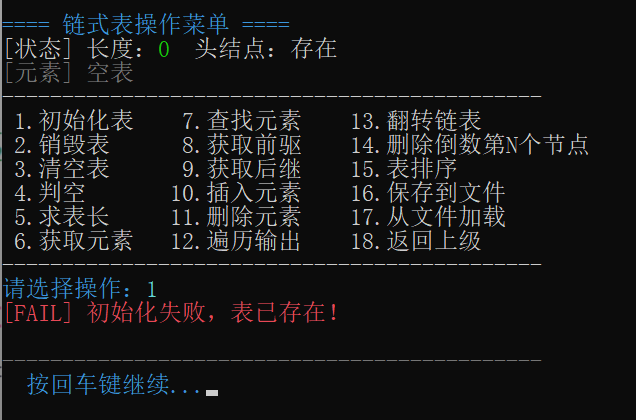
\includegraphics[width=0.5\linewidth]{界面示例1.png}
	\caption{界面示例}
\end{figure}


\subsubsection{设计总结}



整个控制台前端具有以下工程特点：
\begin{itemize}
    \item \textbf{视觉一致性}：通过 \texttt{printTitle}、\texttt{pressEnter} 等辅助函数统一了各菜单的页眉、页脚和分隔样式，用户体验连贯。
    \item \textbf{色彩语义化}：固定的颜色编码,在测试时可凭颜色直觉判断操作结果和状态。
    \item \textbf{资源友好}：全部使用 Windows 原生控制台，程序体积小，响应迅速。
\end{itemize}
\newpage
\begin{figure}[htb]
	\centering
	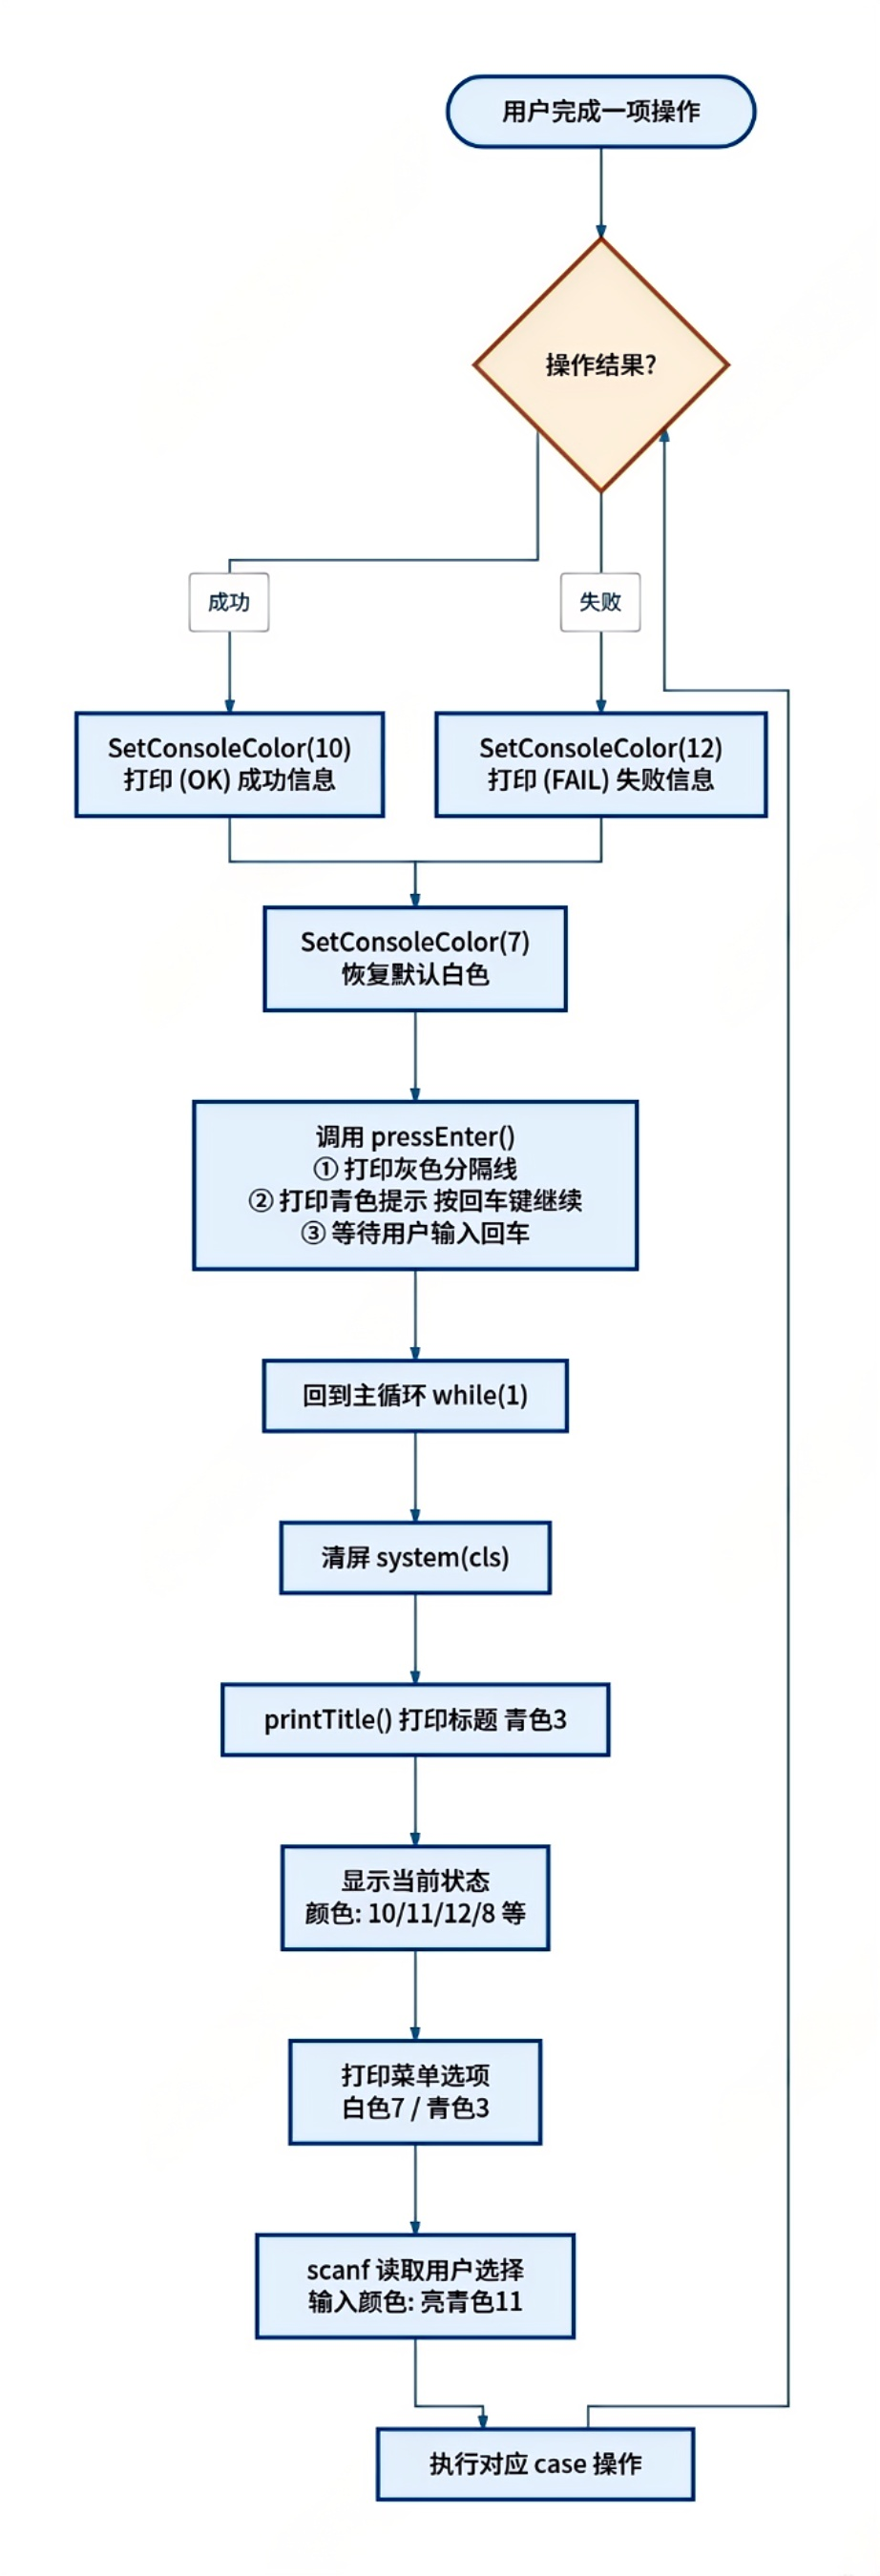
\includegraphics[width=0.4\linewidth]{前端.png}
	\caption{前端控制流}
\end{figure}


\vspace{-2em}
\subsection{实验二小结}
\vspace{-1em}
本实验全面掌握了单链表的链式存储结构与操作。核心收获：(1)头节点（哨兵节点）统一了空表/非空表的操作逻辑；(2)插入（搭桥）、删除（绕行）、逆置（头插法）构成三大指针操作范式；(3)快慢指针法以$O(n)$时间一次遍历解决问题；(4)三层架构+多表管理的设计可推广至后续实验。
\vspace{-2em}
\subsection{程序测试结果截图示例}
\vspace{-1em}
以下按照实验的测试要求，依次展示线性表综合管理系统的各项功能运行结果。测试环境为 Windows 11 + MinGW g++，程序在命令提示符窗口中运行。


\begin{figure}[!htb]
\centering

\includegraphics[width=0.75\textwidth]{images/t2_exam4_image1.png}\vspace{2pt}
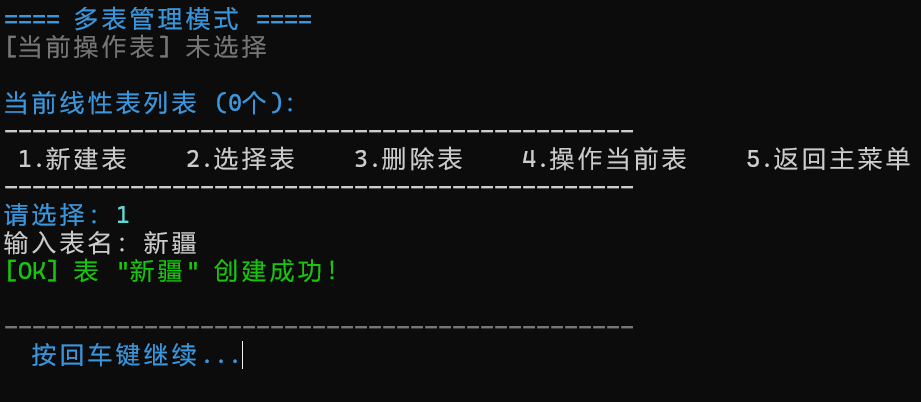
\includegraphics[width=0.75\textwidth]{images/t2_exam4_image2.png}\vspace{2pt}
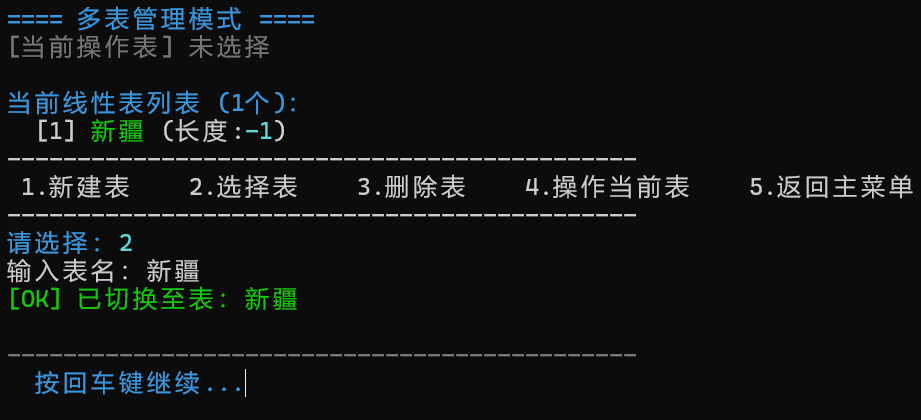
\includegraphics[width=0.75\textwidth]{images/t2_exam4_image3.png}\vspace{2pt}
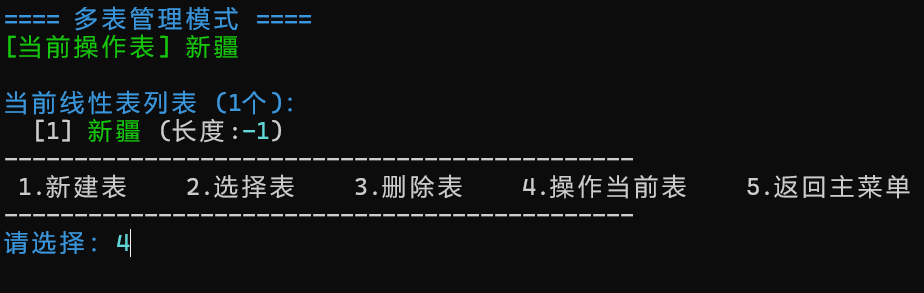
\includegraphics[width=0.75\textwidth]{images/t2_exam4_image4.png}\vspace{2pt}
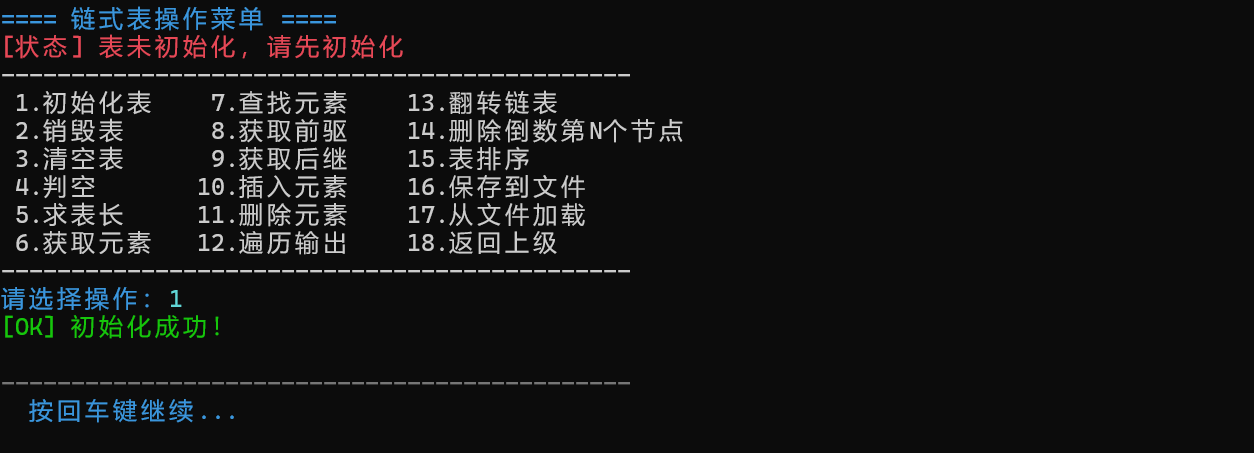
\includegraphics[width=0.75\textwidth]{images/t2_exam4_image5.png}
\caption{多表管理模式下创建名为"新疆"的线性表，进入单表操作菜单并初始化链表}
\label{fig:exam1-create-xj}
\end{figure}
\newpage
\begin{figure}[!htb]
\centering
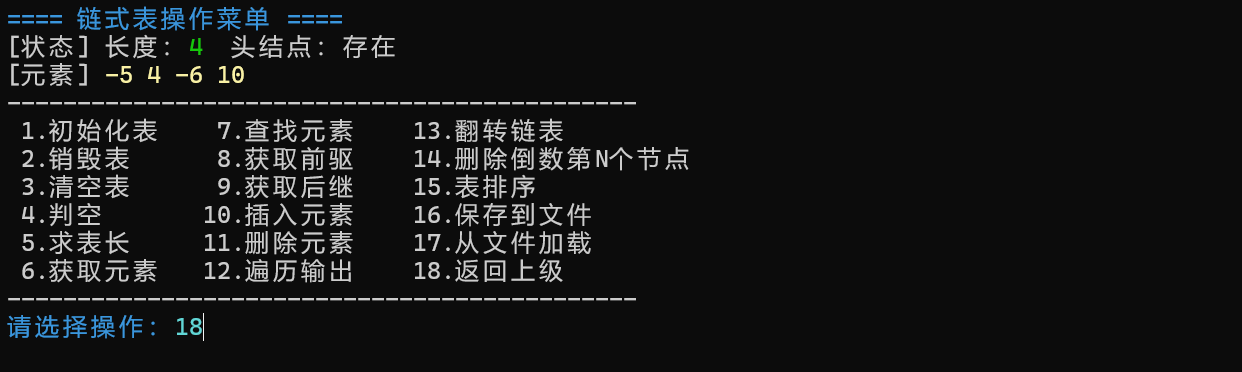
\includegraphics[width=0.75\textwidth]{images/t2_exam4_image19.png}\vspace{2pt}

\includegraphics[width=0.75\textwidth]{images/t2_exam4_image20.png}\vspace{2pt}
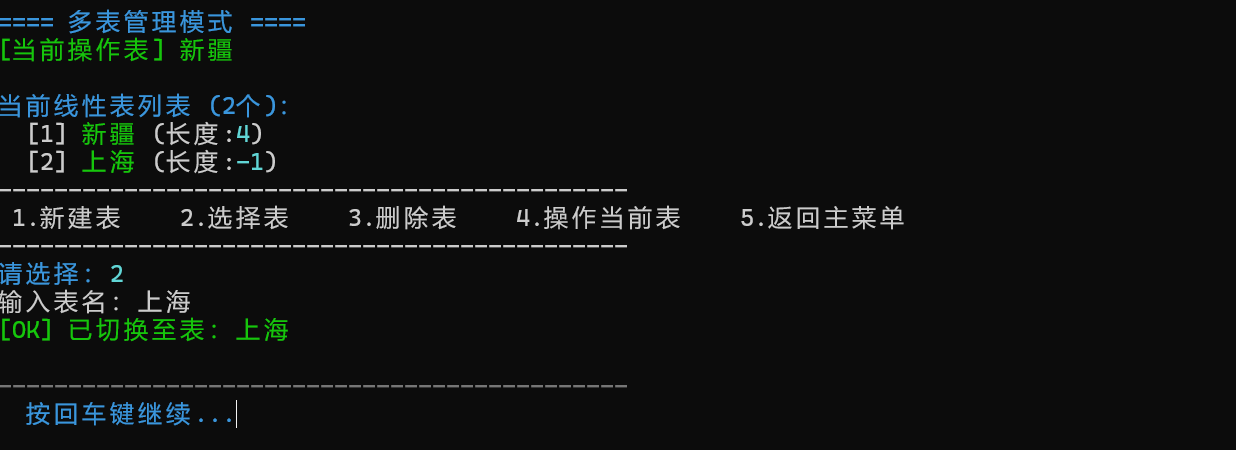
\includegraphics[width=0.75\textwidth]{images/t2_exam4_image21.png}\vspace{2pt}
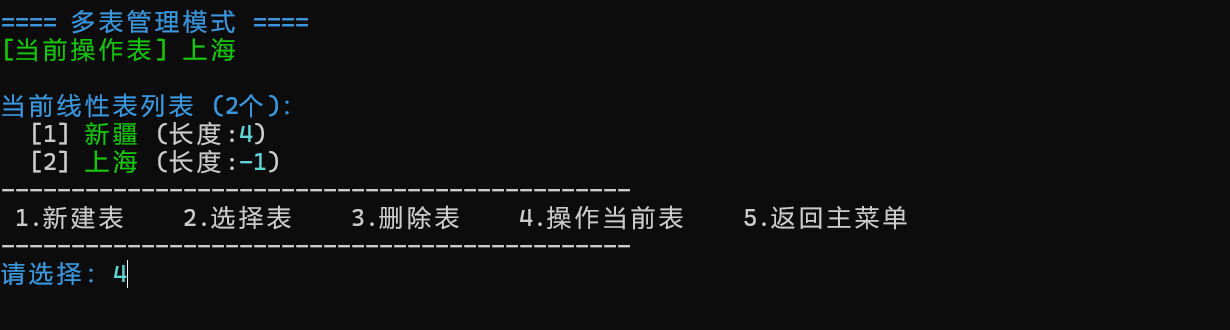
\includegraphics[width=0.75\textwidth]{images/t2_exam4_image22.png}\vspace{2pt}
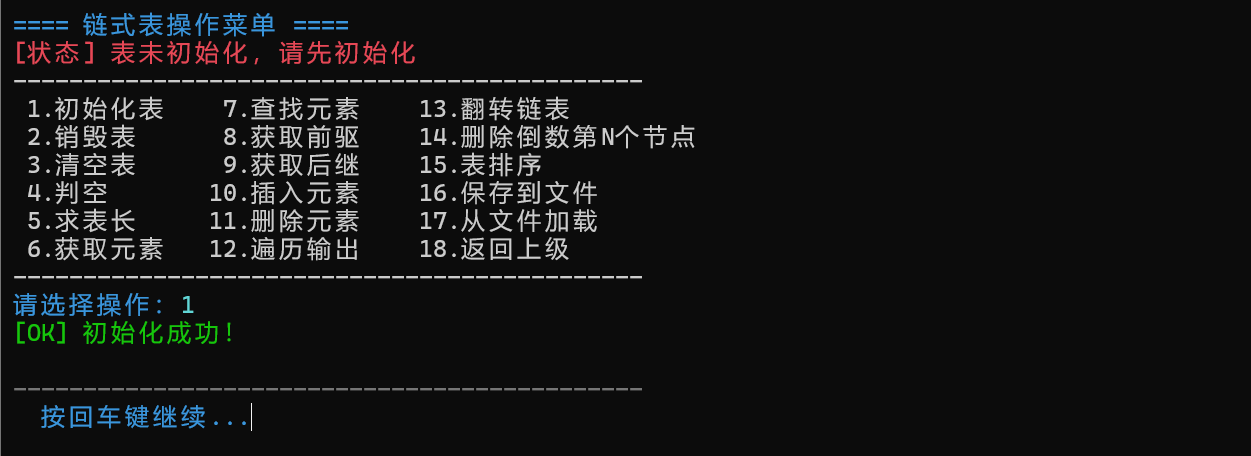
\includegraphics[width=0.75\textwidth]{images/t2_exam4_image23.png}
\caption{多表管理模式下创建名为"上海"的线性表，进入单表操作菜单并初始化链表}
\label{fig:exam1-create-sh}
\end{figure}


\begin{figure}[!htb]
\centering
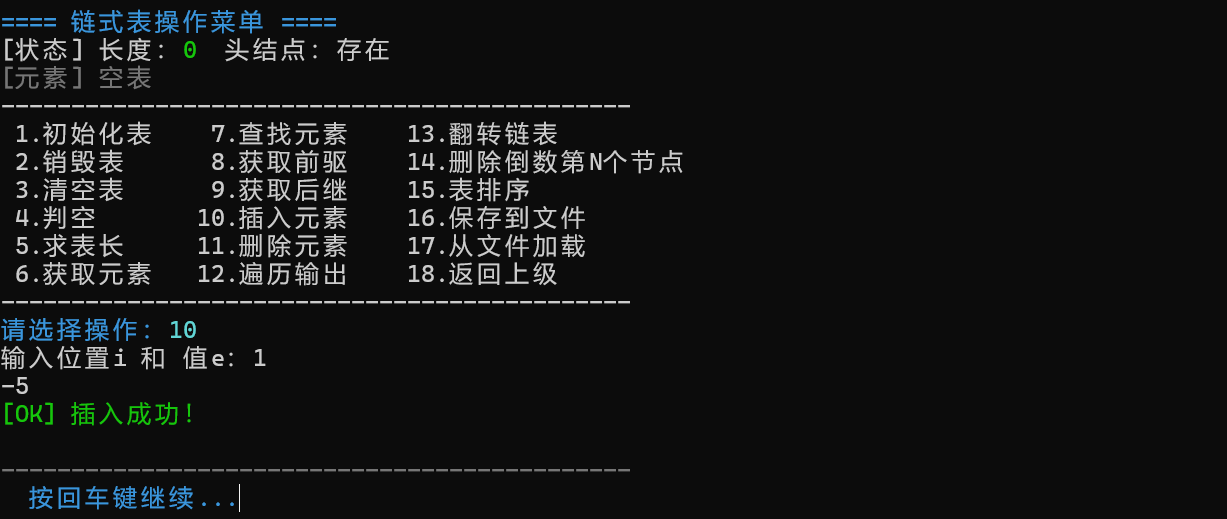
\includegraphics[width=0.75\textwidth]{images/t2_exam4_image6.png}\vspace{2pt}
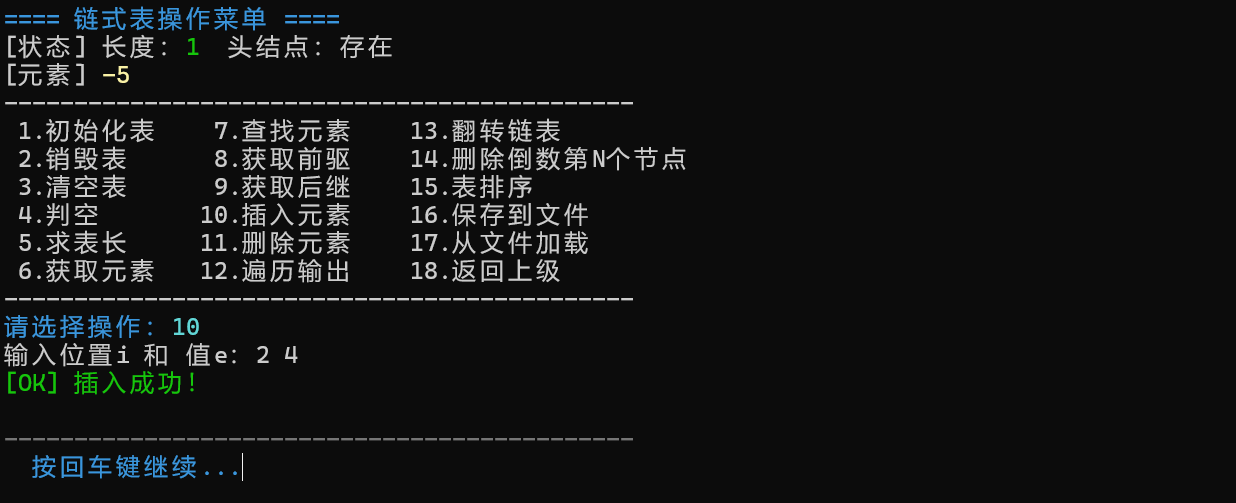
\includegraphics[width=0.75\textwidth]{images/t2_exam4_image7.png}\vspace{2pt}
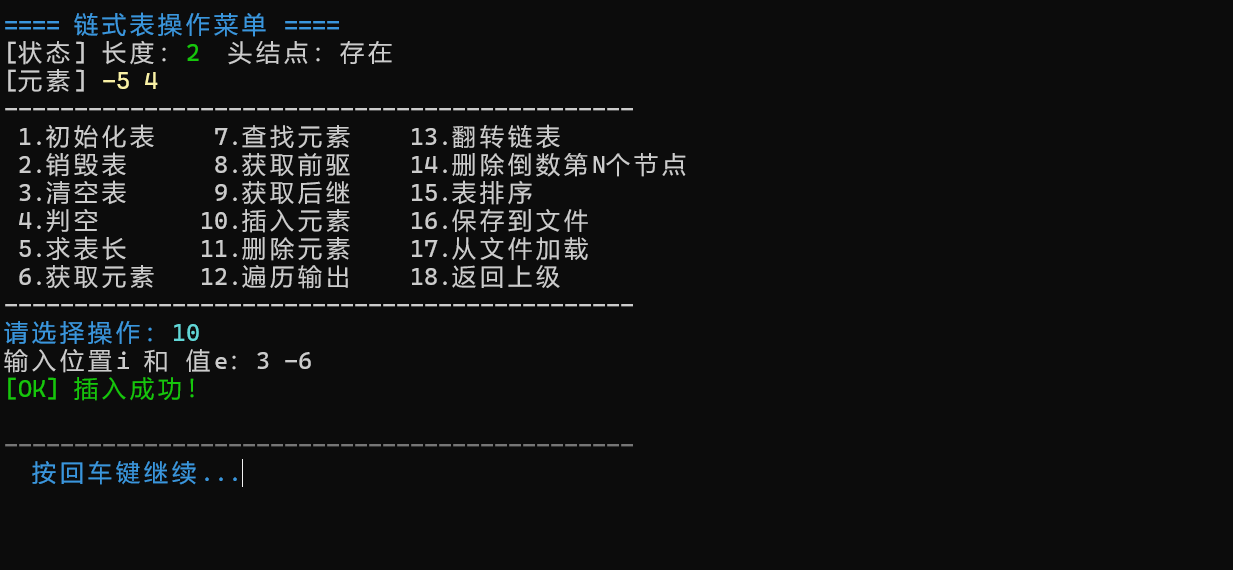
\includegraphics[width=0.75\textwidth]{images/t2_exam4_image8.png}\vspace{2pt}
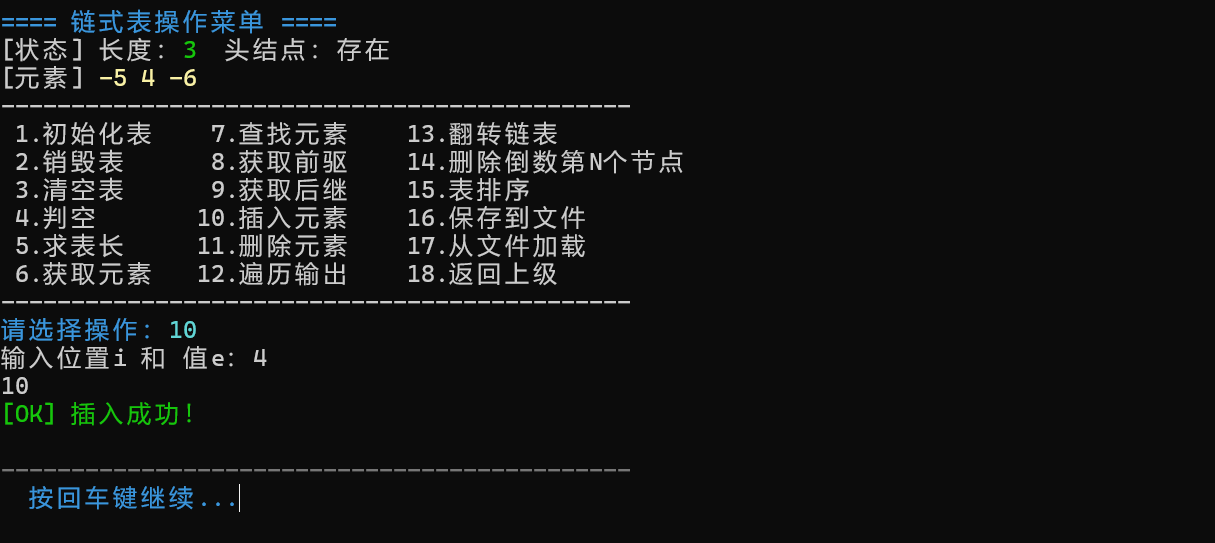
\includegraphics[width=0.75\textwidth]{images/t2_exam4_image9.png}
\caption{向表"新疆"中依次按位插入数据 $[-5,\;4,\;-6,\;10]$，每次插入后遍历查看结果}
\label{fig:exam1-insert-xj}
\end{figure}
\newpage
\begin{figure}[!htb]
\centering
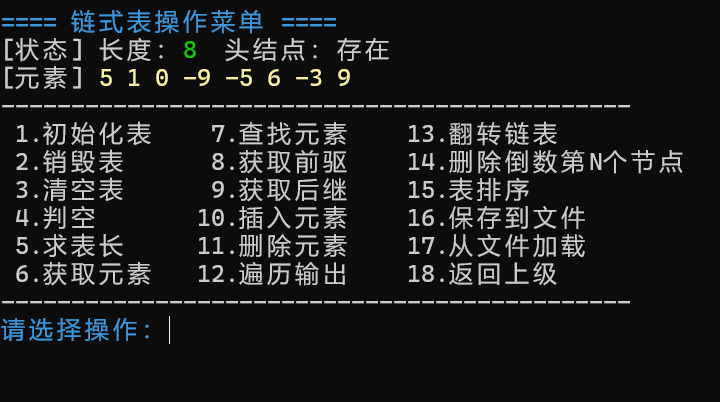
\includegraphics[width=0.75\textwidth]{images/t2_exam4_image33.png}\vspace{2pt}
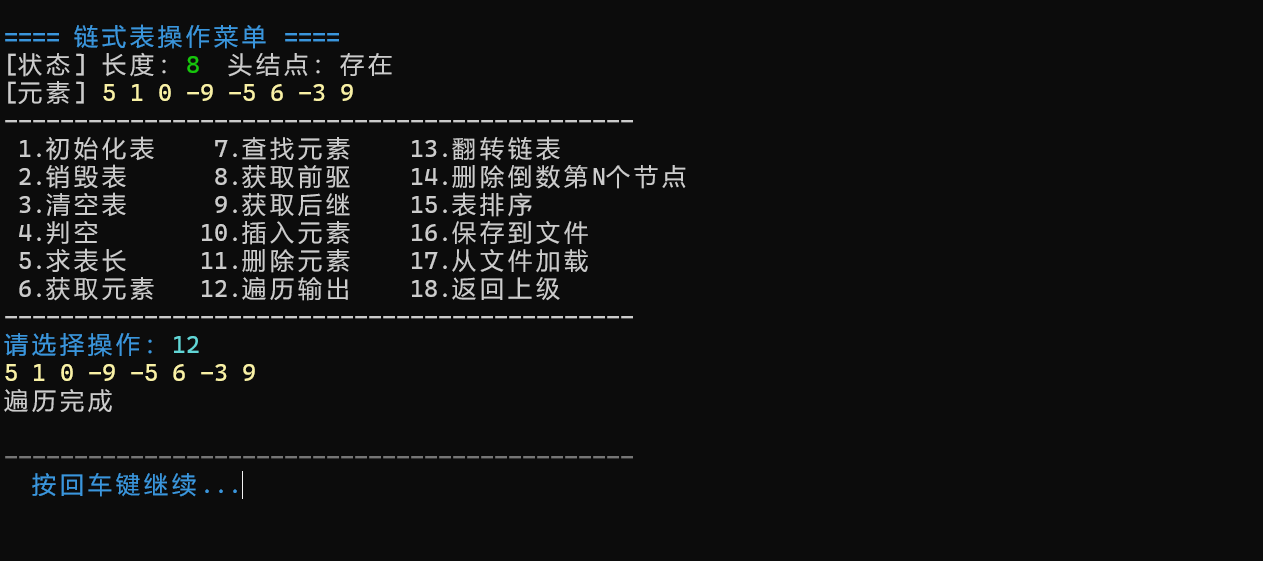
\includegraphics[width=0.75\textwidth]{images/t2_exam4_image34.png}
\caption{向表"上海"中重新按位插入 $[5,\;1,\;0,\;-9,\;-5,\;6,\;-3,\;9]$ 共8个元素并遍历}
\label{fig:exam1-insert-sh}
\end{figure}


\begin{figure}[!htb]
\centering
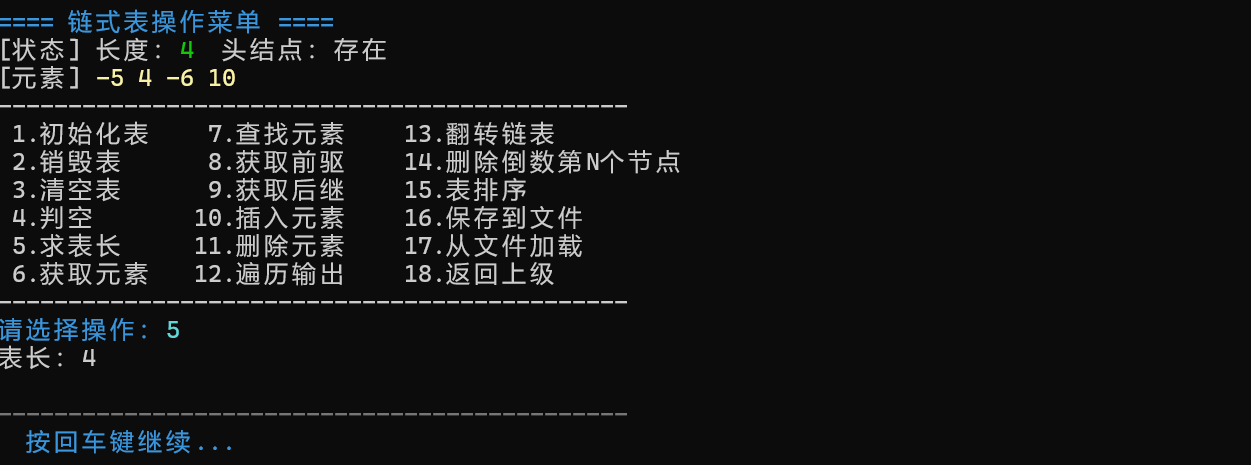
\includegraphics[width=0.75\textwidth]{images/t2_exam4_image10.png}\vspace{2pt}
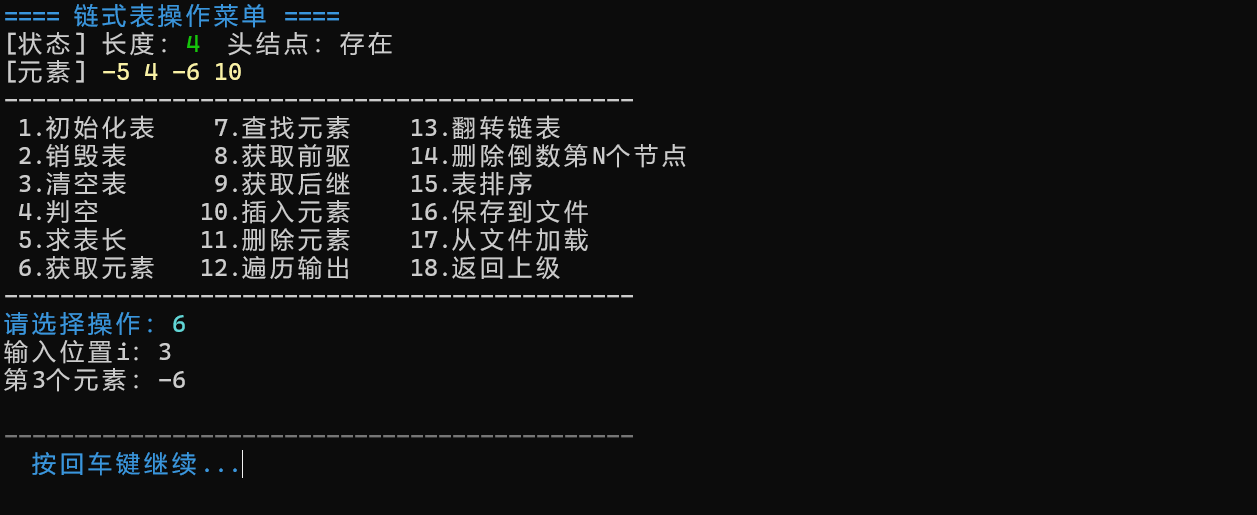
\includegraphics[width=0.75\textwidth]{images/t2_exam4_image11.png}\vspace{2pt}
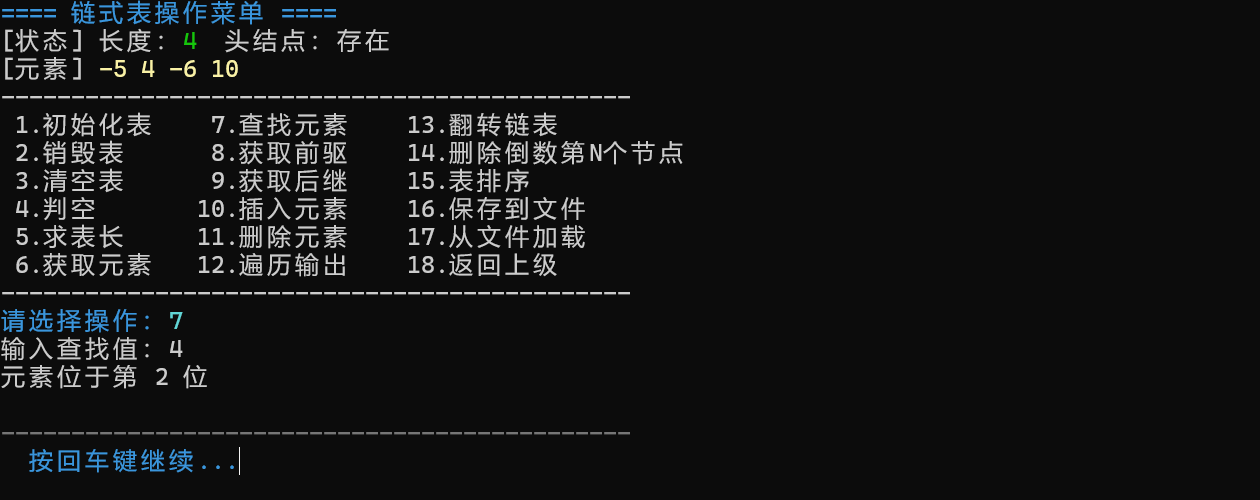
\includegraphics[width=0.75\textwidth]{images/t2_exam4_image12.png}
\caption{依次测试：求表"新疆"的长度、按位序获取第3个元素、按值定位元素4的位序}
\label{fig:exam1-query-basic}
\end{figure}
\newpage
\begin{figure}[!htb]
\centering
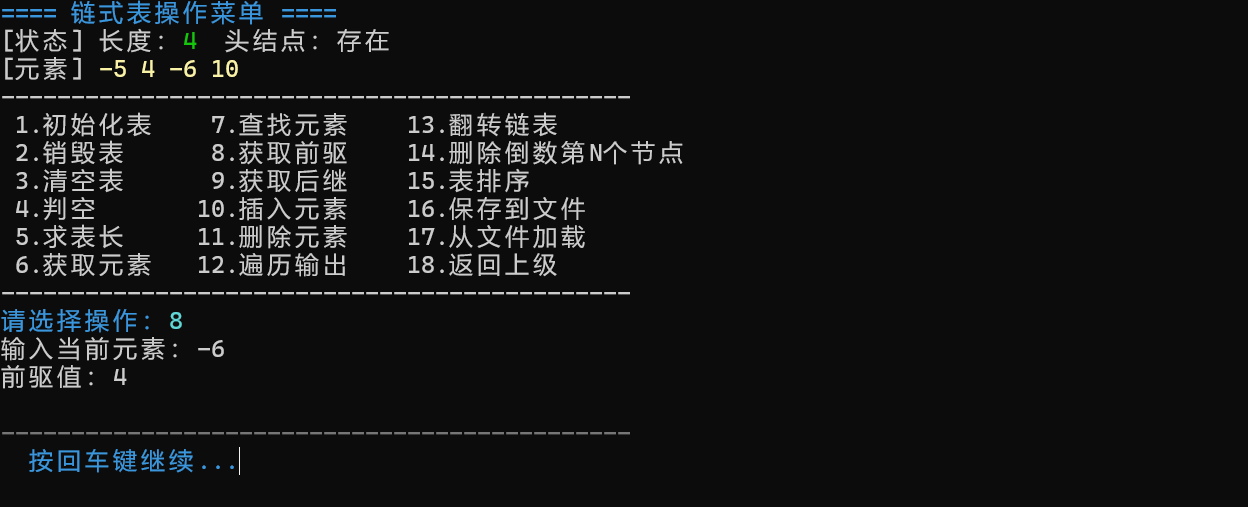
\includegraphics[width=0.75\textwidth]{images/t2_exam4_image13.png}\vspace{2pt}
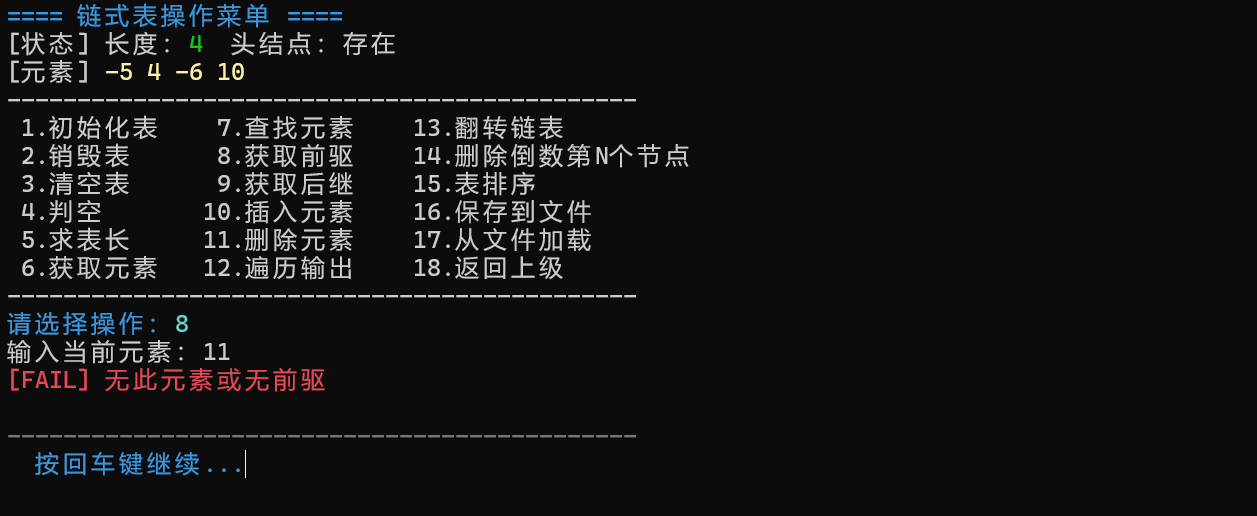
\includegraphics[width=0.75\textwidth]{images/t2_exam4_image14.png}\vspace{2pt}
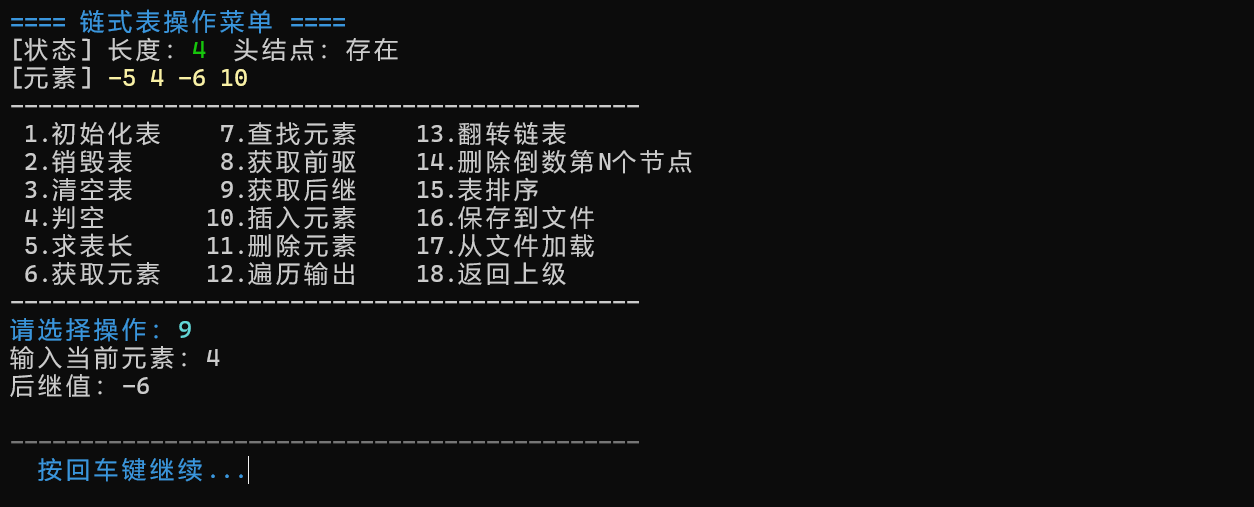
\includegraphics[width=0.75\textwidth]{images/t2_exam4_image15.png}\vspace{2pt}
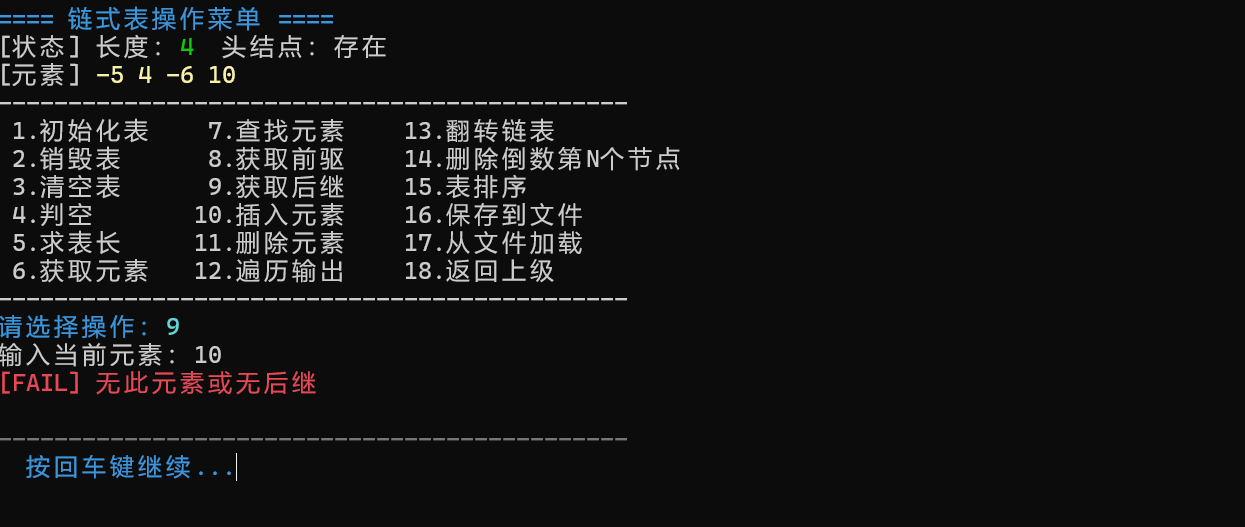
\includegraphics[width=0.75\textwidth]{images/t2_exam4_image16.png}
\caption{前驱与后继测试：获取$-6$的前驱（成功）；获取$11$的前驱（失败——元素不存在）；获取$4$的后继（成功）；获取$10$的后继（失败——最后一个元素无后继）}
\label{fig:exam1-query-pn}
\end{figure}
\newpage

\begin{figure}[!htb]
\centering
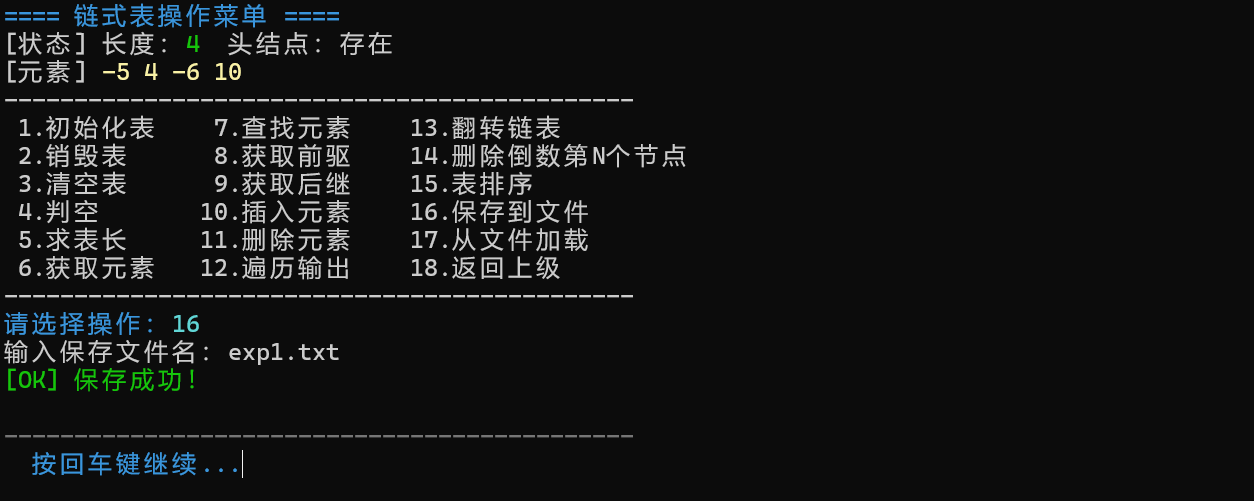
\includegraphics[width=0.75\textwidth]{images/t2_exam4_image17.png}\vspace{2pt}
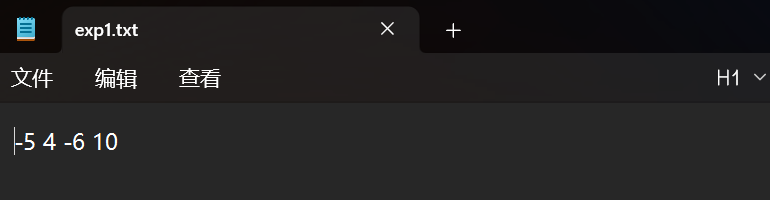
\includegraphics[width=0.75\textwidth]{images/t2_exam4_image18.png}
\caption{将表"新疆"保存至文件 \texttt{exp1.txt}；显示生成的文本文件内容}
\label{fig:exam1-file-save}
\end{figure}

\begin{figure}[!htb]
\centering
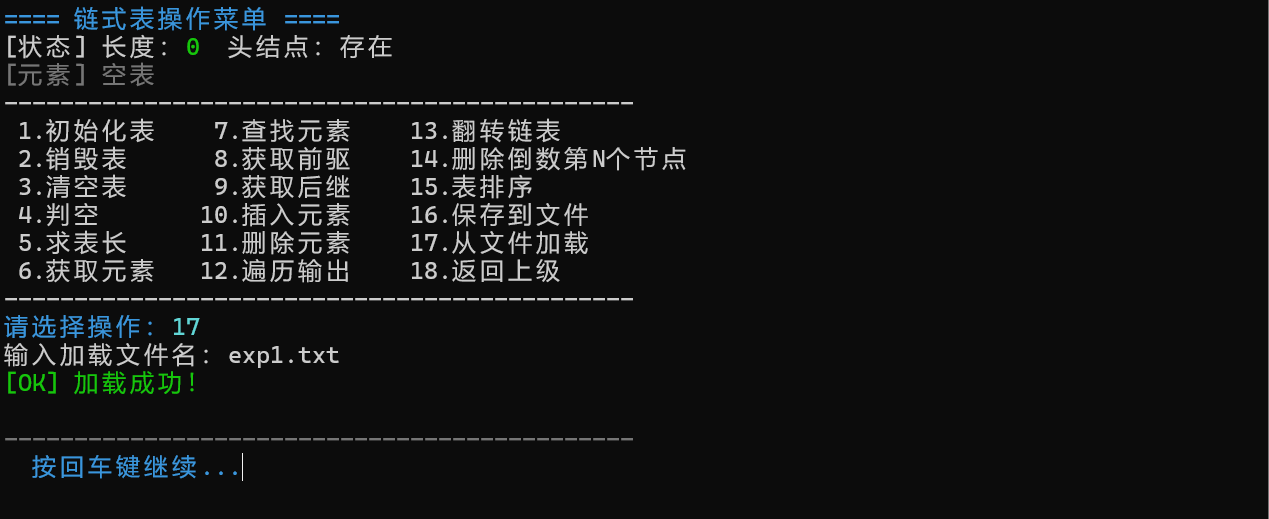
\includegraphics[width=0.75\textwidth]{images/t2_exam4_image24.png}
\caption{表"上海"从文件 \texttt{exp1.txt} 中加载数据（尾插法建表，恢复 $[-5,\;4,\;-6,\;10]$）}
\label{fig:exam1-file-load}
\end{figure}


\begin{figure}[!htb]
\centering
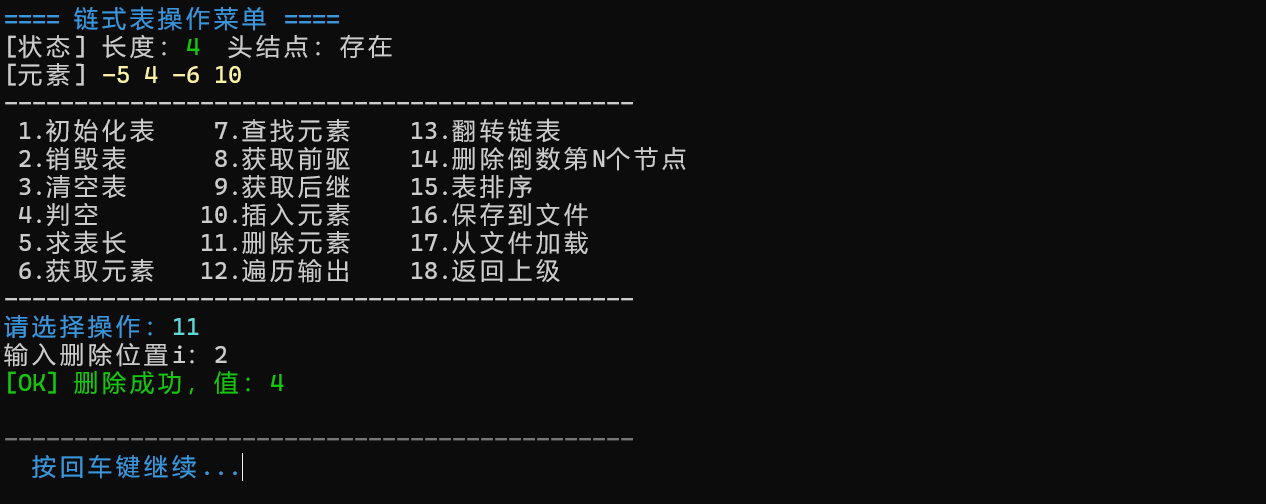
\includegraphics[width=0.75\textwidth]{images/t2_exam4_image25.png}\vspace{2pt}
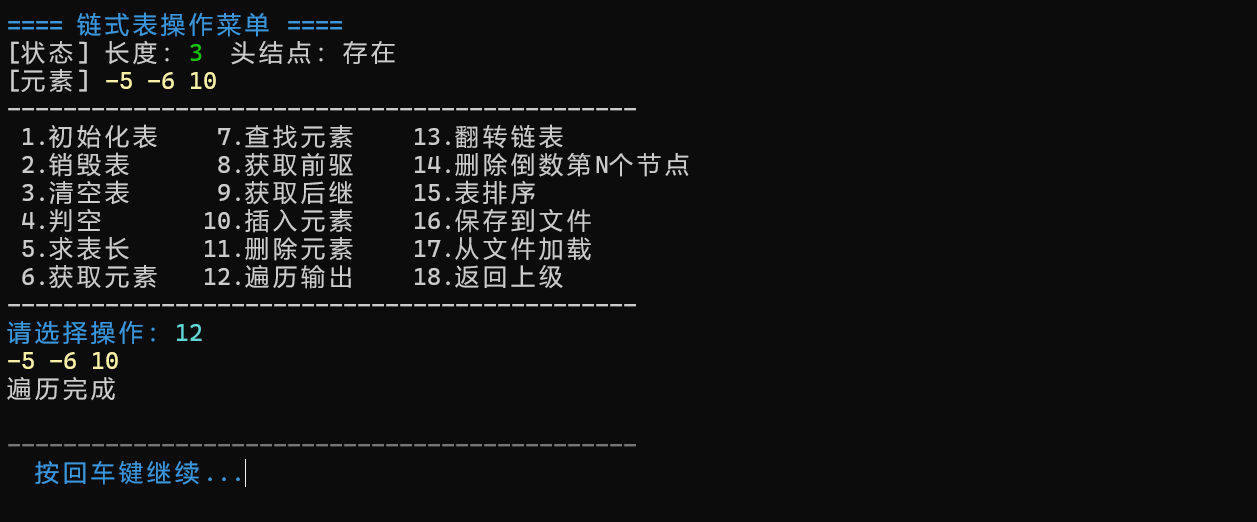
\includegraphics[width=0.75\textwidth]{images/t2_exam4_image26.png}\vspace{2pt}
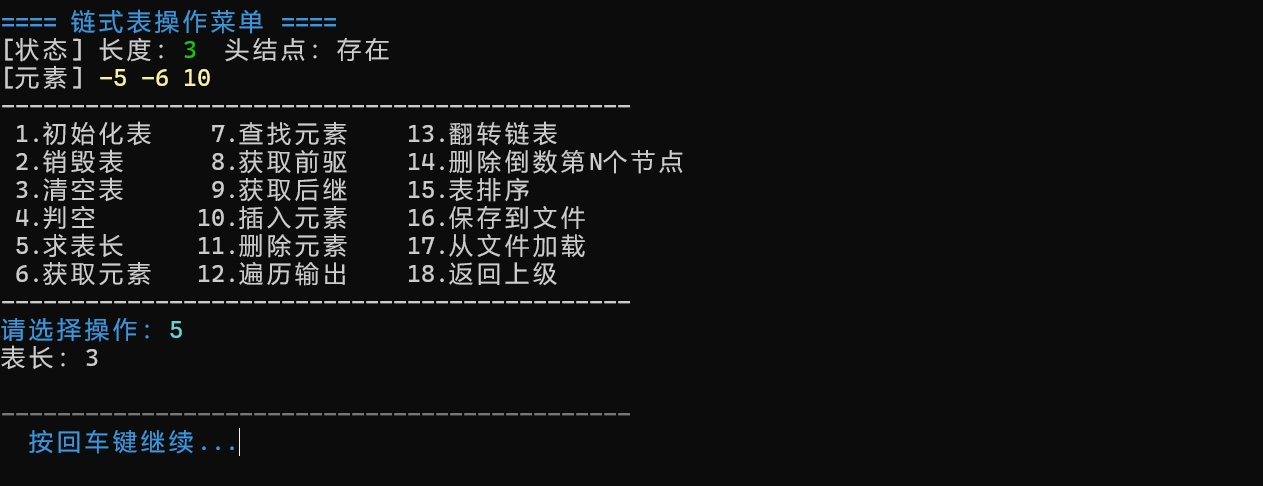
\includegraphics[width=0.75\textwidth]{images/t2_exam4_image27.png}
\caption{依次测试：删除表"上海"的第2个元素（$-6$→$4$→$10$ → 删除位序2的$4$后变为 $-6$→$10$）；遍历查看；求长度}
\label{fig:exam1-del-trav-len}
\end{figure}

\begin{figure}[!htb]
\centering
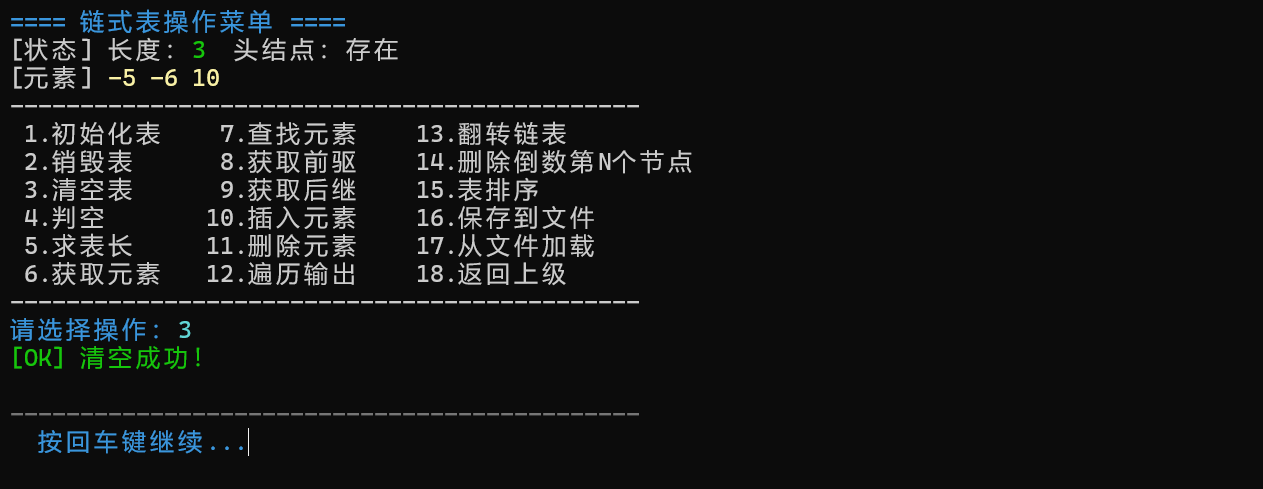
\includegraphics[width=0.75\textwidth]{images/t2_exam4_image28.png}\vspace{2pt}
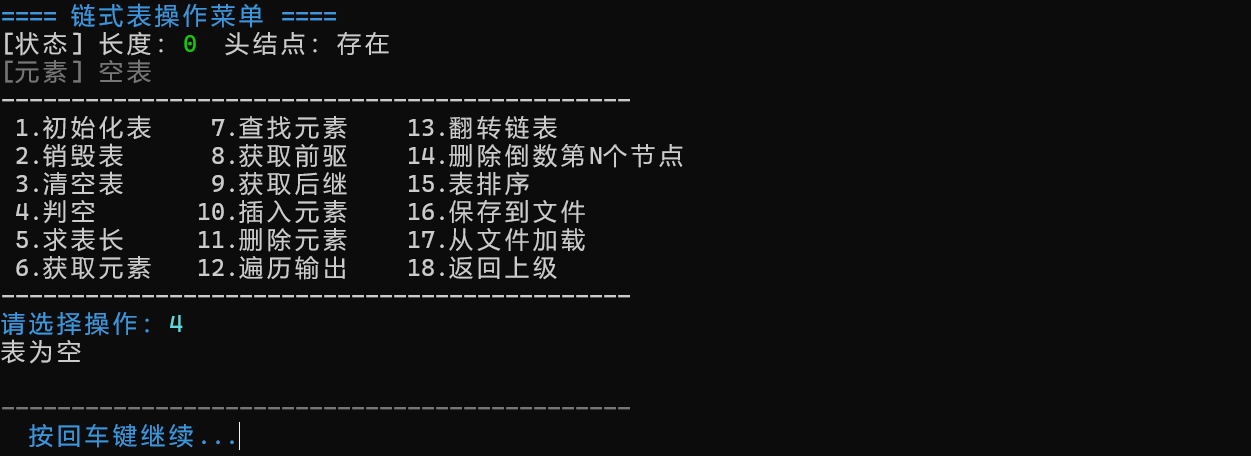
\includegraphics[width=0.75\textwidth]{images/t2_exam4_image29.png}
\caption{清空表"上海"（保留头节点）；判定空表——返回TRUE}
\label{fig:exam1-clear-empty}
\end{figure}


\begin{figure}[!htb]
\centering
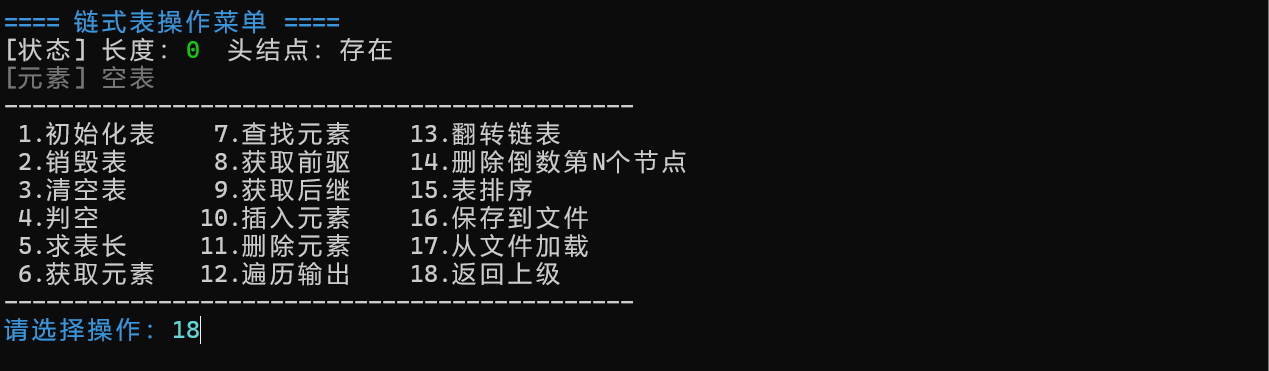
\includegraphics[width=0.75\textwidth]{images/t2_exam4_image30.png}\vspace{2pt}
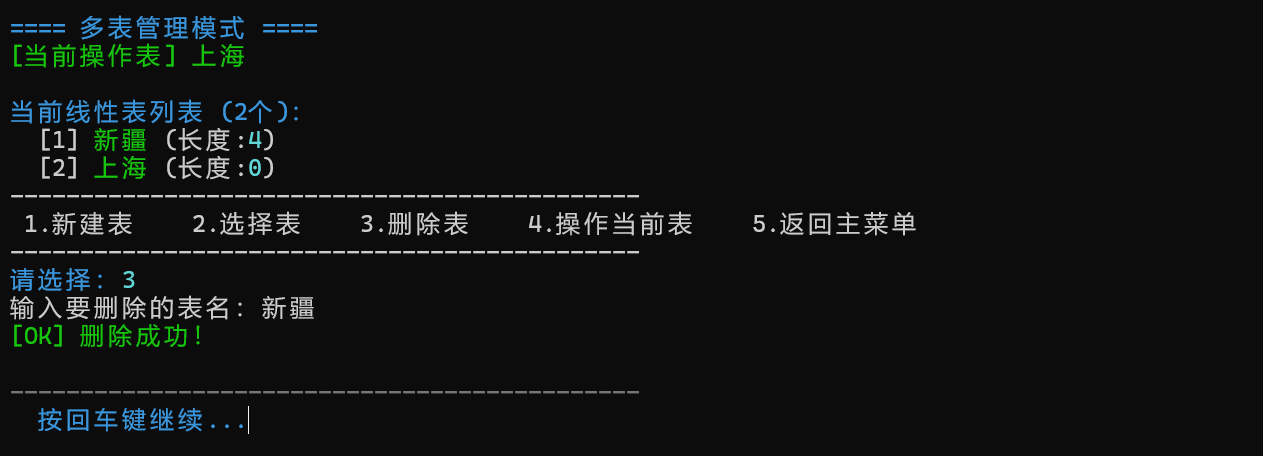
\includegraphics[width=0.75\textwidth]{images/t2_exam4_image31.png}\vspace{2pt}
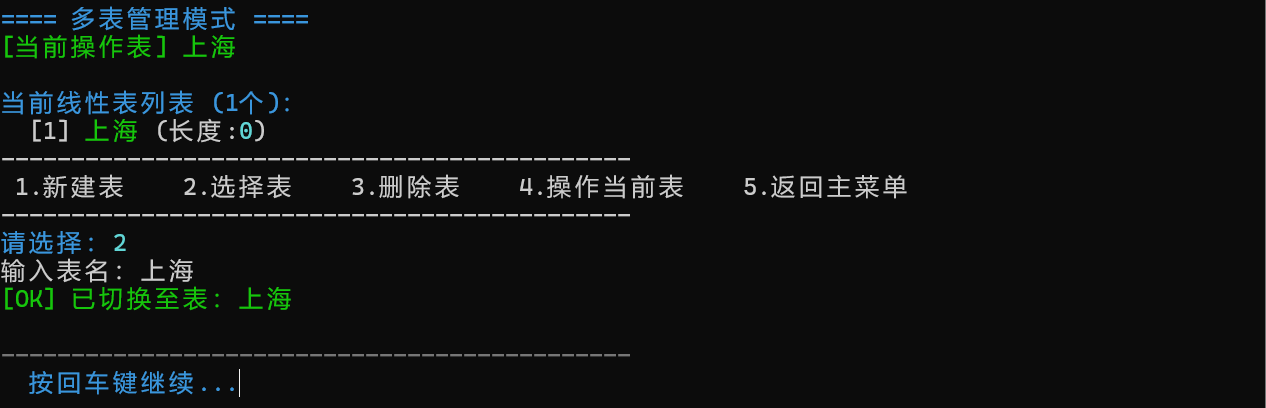
\includegraphics[width=0.75\textwidth]{images/t2_exam4_image32.png}
\caption{多表管理：删除表"新疆"（先释放链表再移除条目）；查找表"上海"的位序}
\label{fig:exam1-multitable}
\end{figure}


\begin{figure}[!htb]
\centering
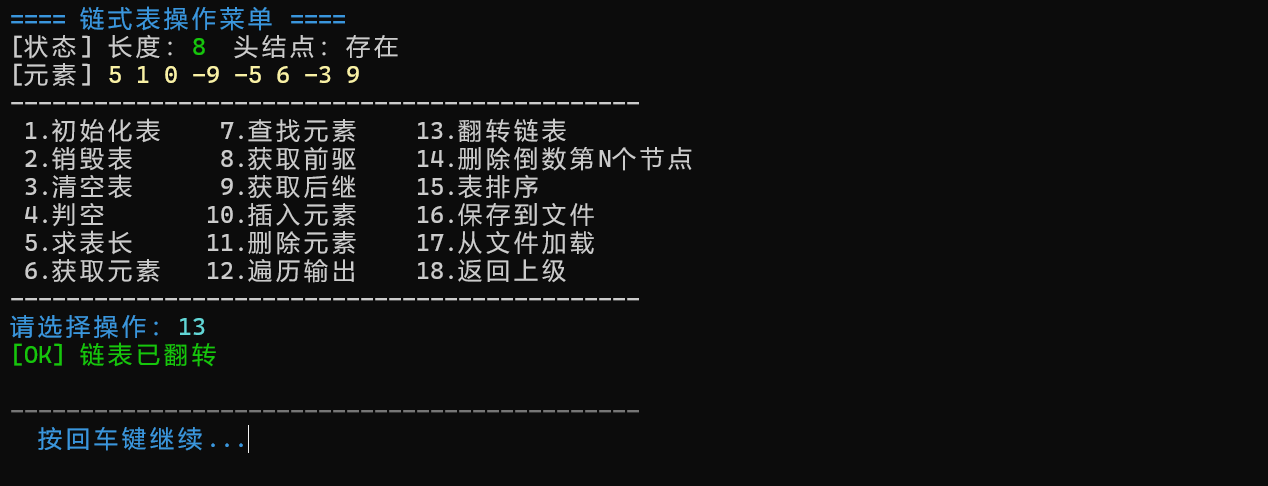
\includegraphics[width=0.75\textwidth]{images/t2_exam4_image35.png}\vspace{2pt}
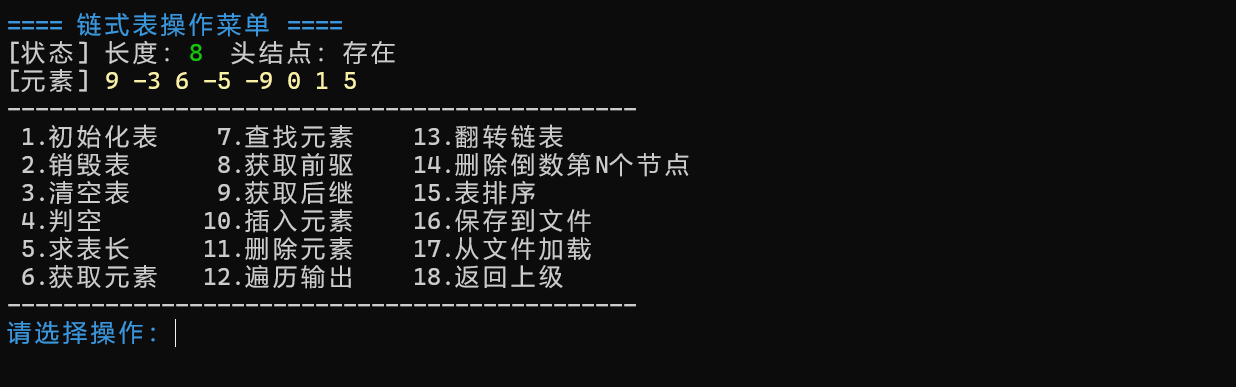
\includegraphics[width=0.75\textwidth]{images/t2_exam4_image36.png}
\caption{链表逆置——表"上海"翻转前：$5\to1\to0\to-9\to-5\to6\to-3\to9$；翻转后：$9\to-3\to6\to-5\to-9\to0\to1\to5$}
\label{fig:exam1-reverse}
\end{figure}

\begin{figure}[!htb]
\centering
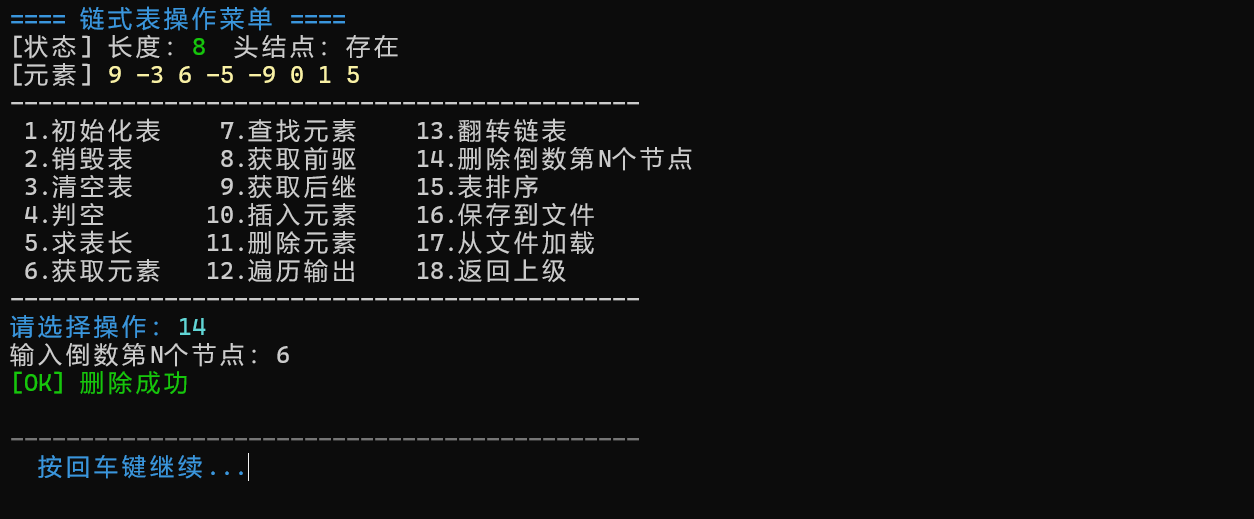
\includegraphics[width=0.75\textwidth]{images/t2_exam4_image37.png}\vspace{2pt}
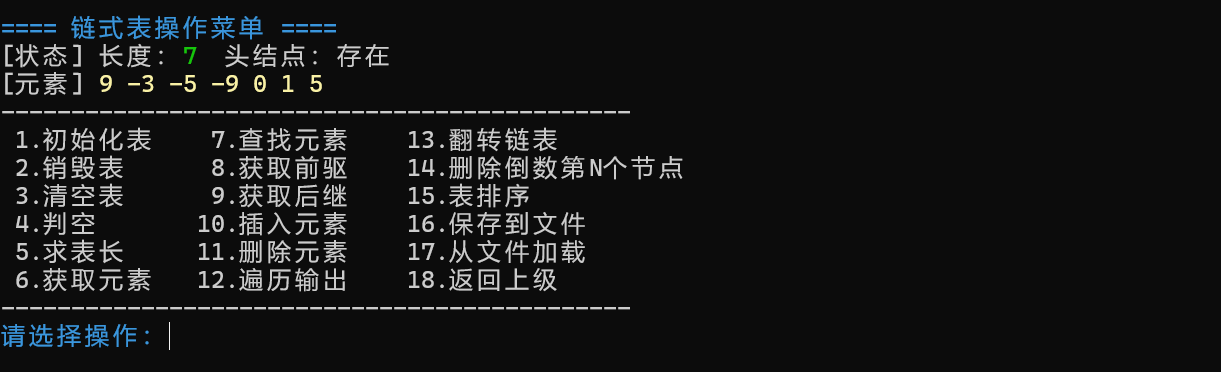
\includegraphics[width=0.75\textwidth]{images/t2_exam4_image38.png}
\caption{快慢指针法删除倒数第6个节点——翻转后的表$9,-3,6,-5,-9,0,1,5$（倒6为$-5$），删除后：$9,-3,6,-9,0,1,5$}
\label{fig:exam1-removenth}
\end{figure}

\begin{figure}[!htb]
\centering
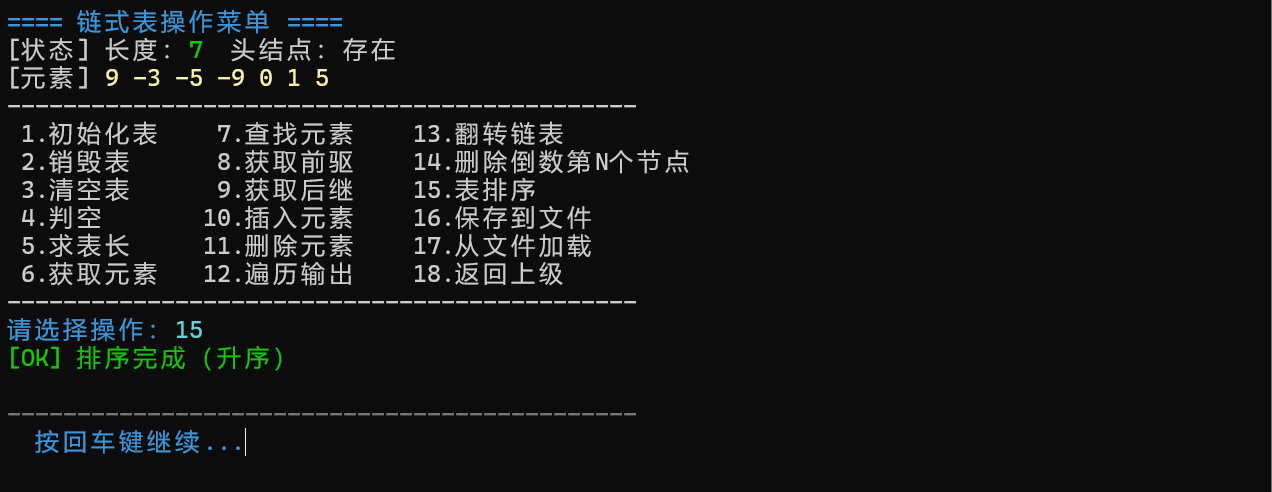
\includegraphics[width=0.75\textwidth]{images/t2_exam4_image39.png}\vspace{2pt}
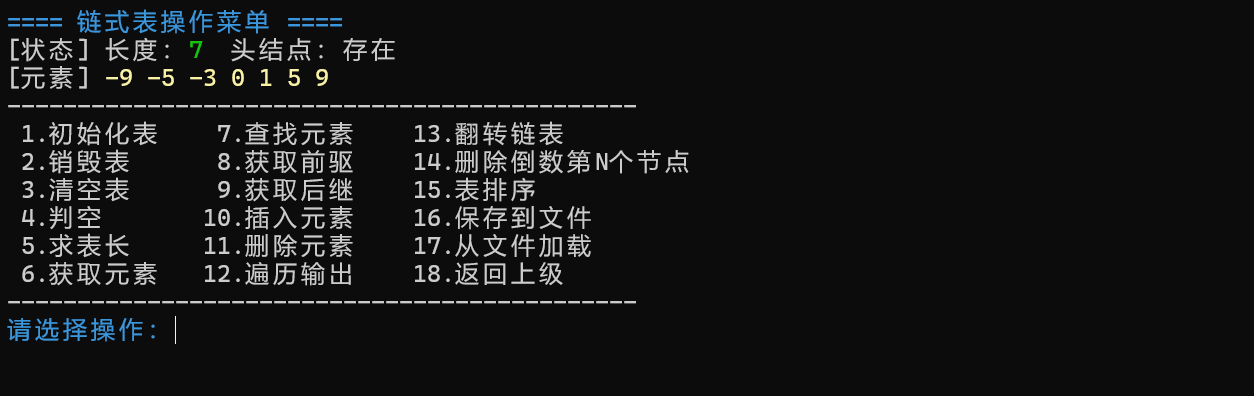
\includegraphics[width=0.75\textwidth]{images/t2_exam4_image40.png}
\caption{冒泡排序——对表"上海"进行升序排列：排序前$9,-3,6,-9,0,1,5$；排序后$-9,-3,0,1,5,6,9$}
\label{fig:exam1-sort}
\end{figure}

\begin{figure}[!htb]
\centering
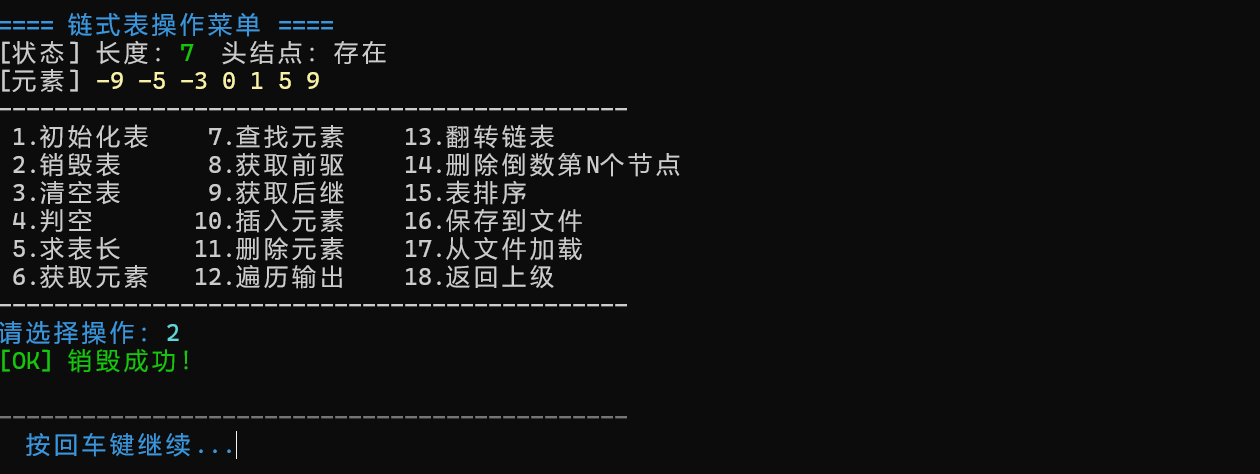
\includegraphics[width=0.75\textwidth]{images/t2_exam4_image41.png}\vspace{2pt}
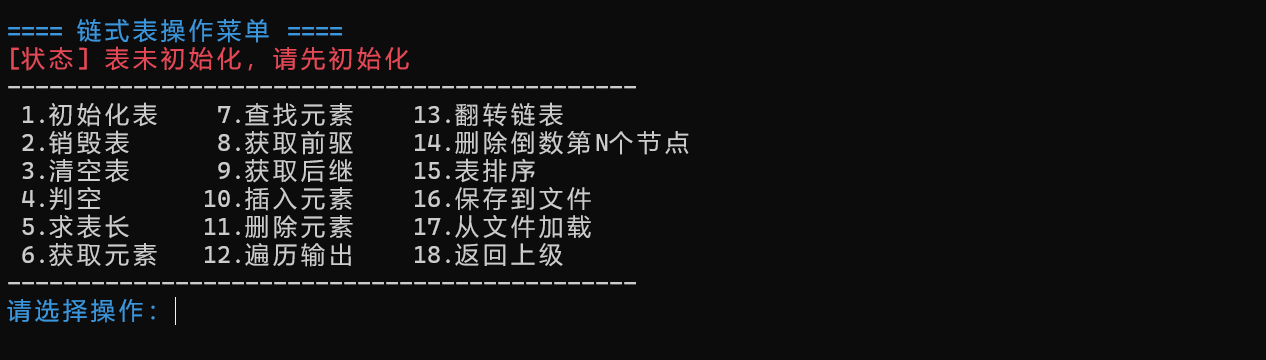
\includegraphics[width=0.75\textwidth]{images/t2_exam4_image42.png}
\caption{销毁表"上海"——释放包括头节点在内的所有内存，销毁后遍历输出为空}
\label{fig:exam1-destroy}
\end{figure}

\newpage






\newpage

%==========================================================================
\section{实验四\quad 基于邻接表的图演示系统}
%==========================================================================

\subsection{实验目的与要求}

\subsubsection{实验目的}
\begin{enumerate}
    \item 深入理解图的邻接表存储结构，掌握与邻接矩阵的适用场景差异
    \item 掌握无向图12个基本操作及DFS/BFS两种遍历算法
    \item 掌握基于BFS的三个应用：最短路径、连通分量、距离筛选
    \item 理解多图管理与文件持久化设计
\end{enumerate}

\subsubsection{实验要求}
实现基于邻接表的图演示系统：单图模式（18项操作）+ 多图管理模式。
功能涵盖建图/销毁、顶点/边增删改查、DFS/BFS遍历、顶点距离<K筛选、最短路径长度、连通分量计数、文件持久化。

\subsection{系统数据结构设计}

\textbf{邻接表}核心思想：为每个顶点维护一个单链表存储所有邻接顶点在数组中的下标。空间$O(n+e)$，稀疏图远优于邻接矩阵$O(n^2)$。

四个嵌套结构体：(1)\textbf{VertexType}——顶点信息(key+others)；(2)\textbf{ArcNode}——弧节点(adjvex+*nextarc)；(3)\textbf{VNode}——邻接表头(data+*firstarc)；(4)\textbf{ALGraph}——完整图(vertices[20]+vexnum+arcnum+kind)。

\begin{figure}[htb]
	\centering
	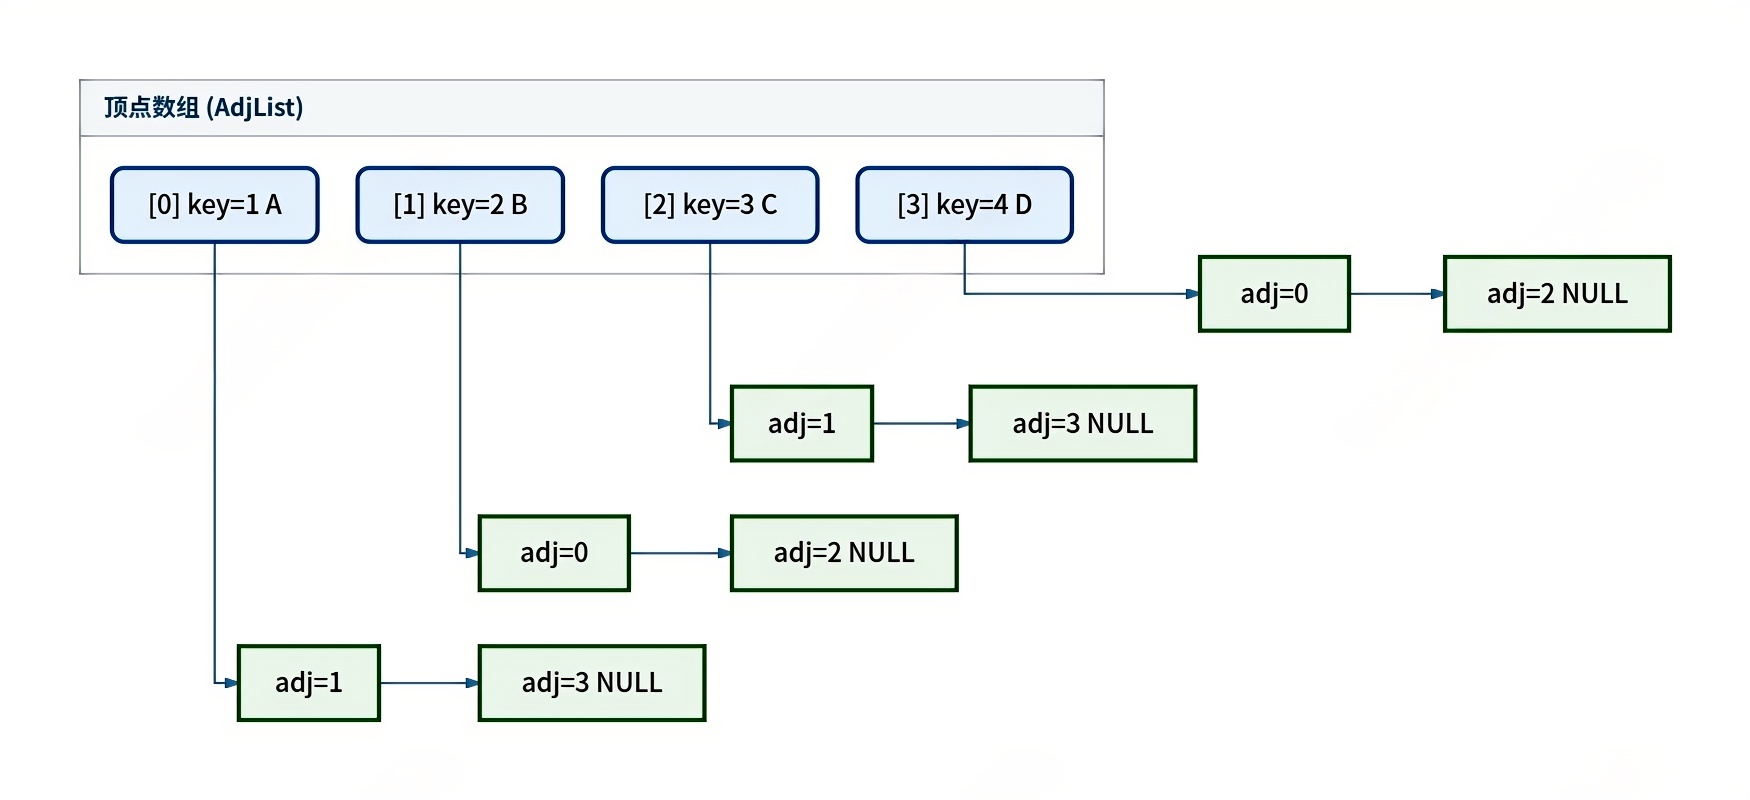
\includegraphics[width=0.85\linewidth]{邻接表.png}
	\caption{邻接表数据结构示意图}
\end{figure}

\subsection{基本功能函数分析}

\subsubsection{CreateGraph(G, V, VR)——创建图}

\begin{quote}\small
\textbf{初始条件：}V是图的顶点集，VR是图的关系集（顶点关键字对序列）。\\
\textbf{操作结果：}按V和VR的定义构造图G，要求顶点关键字唯一。
\end{quote}

\textbf{算法分三步：}(1)遍历V统计顶点数并双重循环检查关键字唯一性（$O(n^2)$，n≤20可接受）；(2)初始化邻接表头——每个顶点的firstarc置NULL；(3)逐条处理VR中的边——对每条边(u,v)，用LocateVex将关键字转为下标，创建两个ArcNode分别用头插法（$O(1)$）插入两个顶点的邻接链表头部，实现无向图的双向邻接。

\begin{figure}[H]
\centering\footnotesize
\resizebox{0.75\textwidth}{!}{
\begin{tikzpicture}[node distance=0.5cm, flowStart, flowProc, flowDec, flowArr]
\node (start) [flowStart] {CreateGraph 入口};
\node (cnt) [flowProc, below=of start] {统计顶点数 vexCount\\（V[i].key != -1）};
\node (c1) [flowDec, below=of cnt] {vexCount==0 或 >MAX?};
\node (bad1) [flowStart, right=3.0cm of c1, fill=orange!30] {返回 ERROR};
\node (dup) [flowDec, below=of c1] {有关键字重复?};
\node (bad2) [flowStart, right=3.0cm of dup, fill=orange!30] {返回 ERROR};
\node (initV) [flowProc, below=of dup] {初始化所有顶点：\\data=V[i], firstarc=NULL};
\node (edgeL) [flowDec, below=of initV] {还有未处理的边?};
\node (loc) [flowProc, below=of edgeL] {LocateVex定位u和v下标\\创建2个ArcNode(头插法)\\G->arcnum++};
\node (kind) [flowProc, below=of loc] {G->kind = UDG};
\node (ok) [flowStart, below=of kind, fill=green!30] {返回 OK};

\draw [flowArr] (start) -- (cnt) -- (c1);
\draw [flowArr] (c1.east) -- node[above]{是} (bad1.west);
\draw [flowArr] (c1) -- node[right]{否} (dup);
\draw [flowArr] (dup.east) -- node[above]{是} (bad2.west);
\draw [flowArr] (dup) -- node[right]{否} (initV);
\draw [flowArr] (initV) -- (edgeL);
\draw [flowArr] (edgeL) -- node[right]{是} (loc);
\draw [flowArr] (loc.west) -- ++(-1.5,0) |- (edgeL.west);
\draw [flowArr] (edgeL.east) -- ++(1.8,0) node[above]{否} |- (kind.east);
% Mermaid 参考: 图27 (CreateGraph建图算法) — 见 Mermaid流程图.txt
\draw [flowArr] (kind) -- (ok);
\end{tikzpicture}
}
\caption{CreateGraph建图算法流程图}
\label{fig:creategraph-flow}
\end{figure}
\newpage
\begin{lstlisting}[label={lst:create-graph}, caption={CreateGraph}]
status CreateGraph(ALGraph *G, VertexType V[], KeyType VR[][2]) {
    int vexCount = 0;
    while (V[vexCount].key != -1) {
        vexCount++;
        if (vexCount > MAX_VERTEX_NUM) return ERROR;
    }
    if (vexCount == 0) return ERROR;
    for (int i = 0; i < vexCount; i++)
        for (int j = i + 1; j < vexCount; j++)
            if (V[i].key == V[j].key) return ERROR;
    G->vexnum = vexCount; G->arcnum = 0;
    for (int i = 0; i < vexCount; i++) {
        G->vertices[i].data = V[i];
        G->vertices[i].firstarc = NULL;
    }
    for (int i = 0; ; i++) {
        KeyType u = VR[i][0]; if (u == -1) break;
        KeyType v = VR[i][1];
        int iu = LocateVex(*G, u), iv = LocateVex(*G, v);
        if (iu == -1 || iv == -1) return ERROR;
        ArcNode *p = (ArcNode*)malloc(sizeof(ArcNode));
        p->adjvex = iv; p->nextarc = G->vertices[iu].firstarc;
        G->vertices[iu].firstarc = p;   // u→v
        ArcNode *q = (ArcNode*)malloc(sizeof(ArcNode));
        q->adjvex = iu; q->nextarc = G->vertices[iv].firstarc;
        G->vertices[iv].firstarc = q;   // v→u
        G->arcnum++;
    }
    G->kind = UDG;
    return OK;
}
\end{lstlisting}

\textbf{两点设计说明：}(1)V和VR是图的\textbf{逻辑定义}形式——V为带终止标记-1的顶点序列，VR为带终止标记(-1,-1)的关键字对序列；算法内部自行将逻辑定义转换为邻接表物理结构；(2)每条边创建两个ArcNode是无向图的本质要求——边在存储上必须是双向的。

\subsubsection{DestroyGraph(G)——销毁图}
% Mermaid 参考: 图28 (DestroyGraph) — 见 Mermaid流程图.txt

\begin{quote}\small
\textbf{初始条件：}图G已存在。\quad\textbf{操作结果：}销毁图G，释放所有ArcNode内存。
\end{quote}

实现分析：两重循环遍历——外层遍历顶点数组，内层遍历每个顶点的弧链表逐节点释放。最后将vexnum和arcnum清零。时间$O(n+e)$。
\begin{figure}[htb]
	\centering
	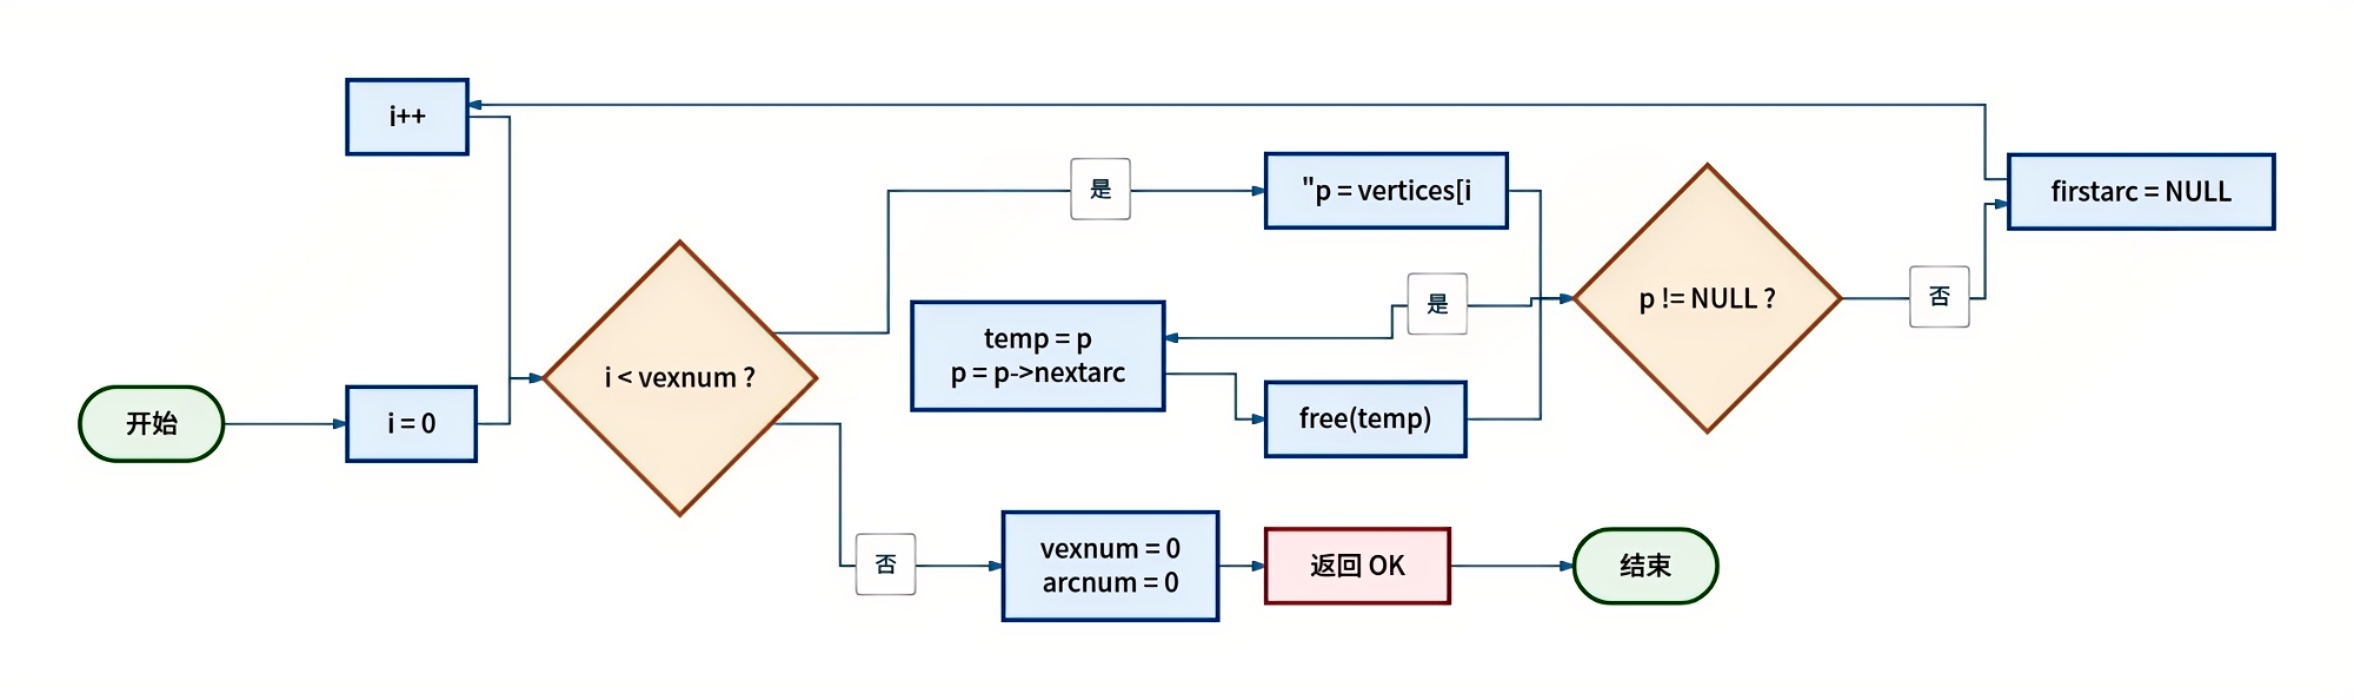
\includegraphics[width=\linewidth]{销毁图.png}
	\caption{销毁图}
\end{figure}
\begin{lstlisting}[label={lst:destroy-graph}, caption={DestroyGraph}]
status DestroyGraph(ALGraph *G) {
    for (int i = 0; i < G->vexnum; i++) {
        ArcNode *p = G->vertices[i].firstarc;
        while (p != NULL) {
            ArcNode *temp = p;
            p = p->nextarc;
            free(temp);
        }
        G->vertices[i].firstarc = NULL;
    }
    G->vexnum = 0; G->arcnum = 0;
    return OK;
}
\end{lstlisting}
\vspace{-2em}
\subsubsection{LocateVex(G, u)——查找顶点}
% Mermaid 参考: 图29 (LocateVex) — 见 Mermaid流程图.txt
\vspace{-0.5em}
\begin{quote}\small
\textbf{初始条件：}图G存在，u是和G中顶点关键字类型相同的给定值。\\
\textbf{操作结果：}若u在G中存在则返回位序，否则返回-1。
\end{quote}
\vspace{-0.5em}
实现分析：线性扫描顶点数组，比较每个顶点的key字段与u。该函数是许多其他操作的基础原语（CreateGraph、PutVex、InsertArc等均依赖它）。时间$O(n)$。

\begin{lstlisting}[label={lst:locate-vex}, caption={LocateVex}]
int LocateVex(ALGraph G, KeyType u) {
    for (int i = 0; i < G.vexnum; i++)
        if (G.vertices[i].data.key == u) return i;
    return -1;
}
\end{lstlisting}

\subsubsection{PutVex(G, u, value)——顶点赋值}
% Mermaid 参考: 图30 (PutVex) — 见 Mermaid流程图.txt

\begin{quote}\small
\textbf{初始条件：}图G存在，u是和G中顶点关键字类型相同的给定值。\\
\textbf{操作结果：}对关键字为u的顶点赋值value（保持关键字唯一性）。
\end{quote}

实现分析：先LocateVex定位，再检查新值的关键字不与图中其他顶点冲突（跳过自身），最后覆盖顶点的data字段。此函数可用于修改顶点名称等附加信息。时间$O(n)$。
\begin{figure}[htb]
	\centering
	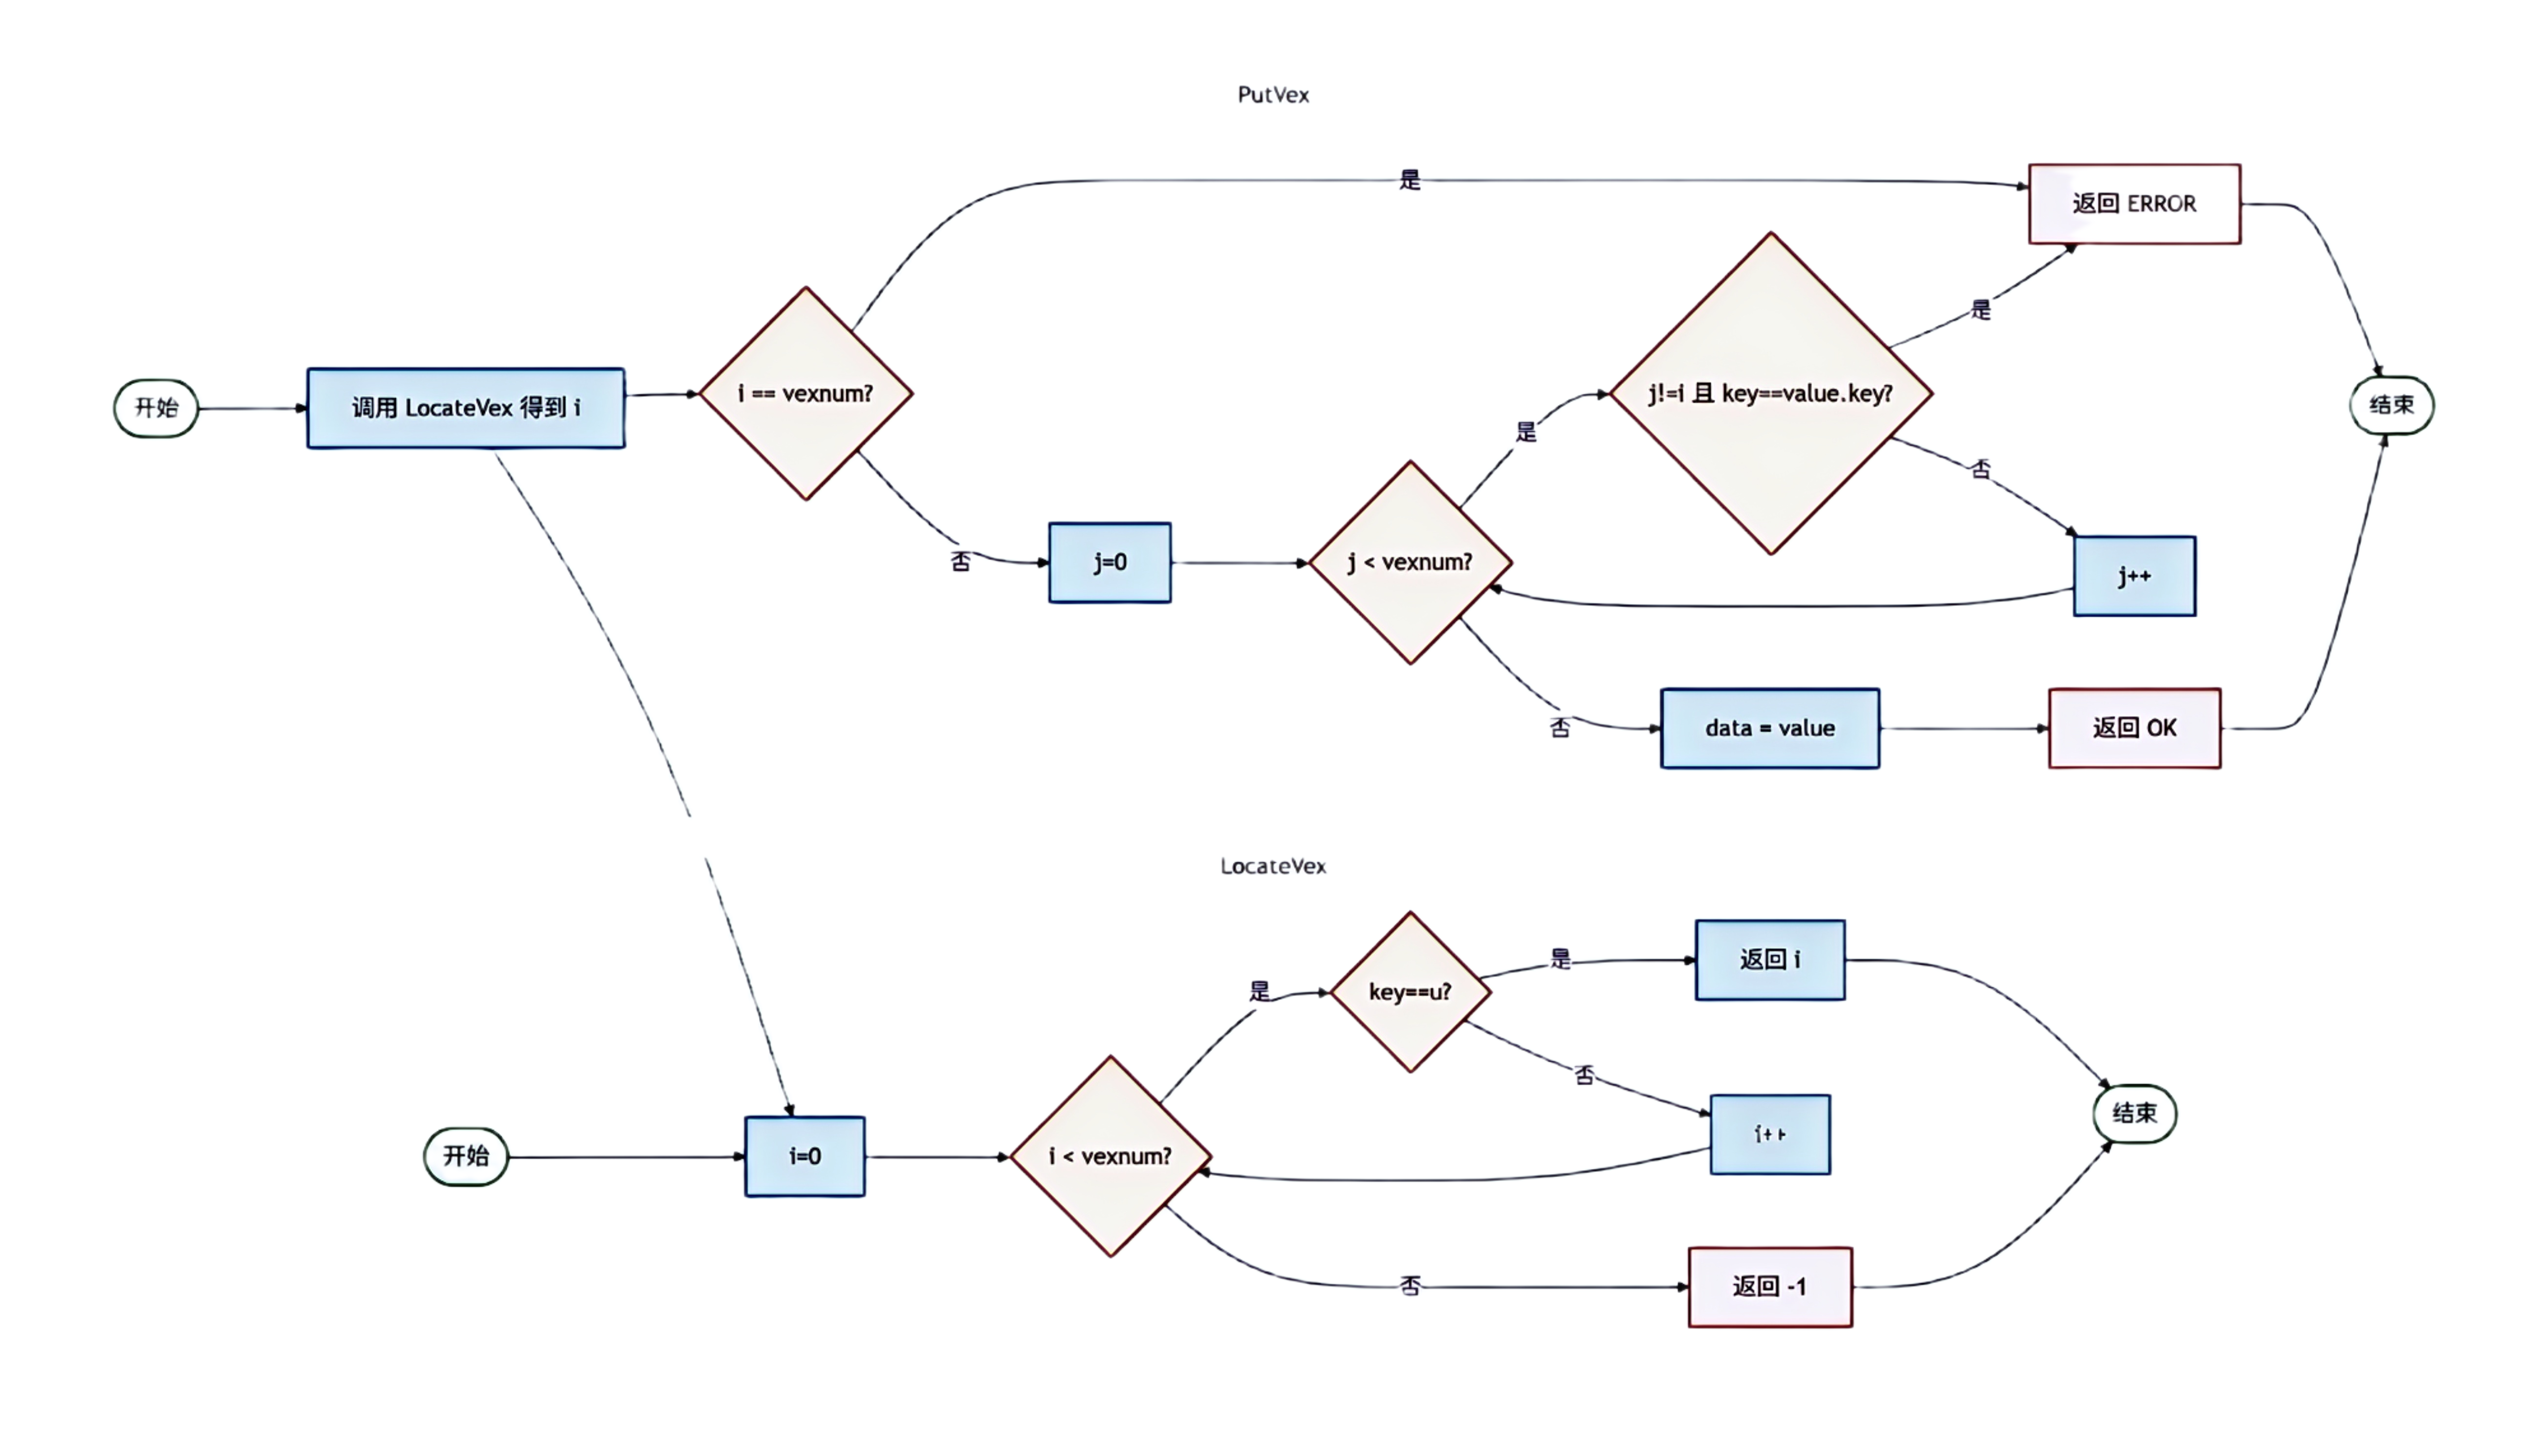
\includegraphics[width=\linewidth]{deepseek_mermaid_20260617_3297aa.png}
	\caption{查找与赋值}
\end{figure}
\begin{lstlisting}[label={lst:put-vex}, caption={PutVex}]
status PutVex(ALGraph *G, KeyType u, VertexType value) {
    int i, j;
    for (i = 0; i < G->vexnum; i++)
        if (G->vertices[i].data.key == u) break;
    if (i == G->vexnum) return ERROR;
    for (j = 0; j < G->vexnum; j++)
        if (j != i && G->vertices[j].data.key == value.key) return ERROR;
    G->vertices[i].data = value;
    return OK;
}
\end{lstlisting}

\subsubsection{FirstAdjVex(G, u)——获得第一邻接点}
% Mermaid 参考: 图31 (FirstAdjVex) — 见 Mermaid流程图.txt

\begin{quote}\small
\textbf{初始条件：}图G存在，u是G中顶点的位序（关键字）。\\
\textbf{操作结果：}返回u对应顶点的第一个邻接顶点的位序（按弧链表顺序），若没有邻接顶点返回-1。
\end{quote}

实现分析：准确来说\textbf{函数接收的是顶点关键字u而非位序}（本实现先用LocateVex转换），检查弧链表是否为空，为空返回-1，否则返回第一个ArcNode的adjvex值。这是BFS/DFS和邻接点遍历的基础原语。时间$O(n)$（LocateVex占主导）。
\begin{figure}[htb]
	\centering
	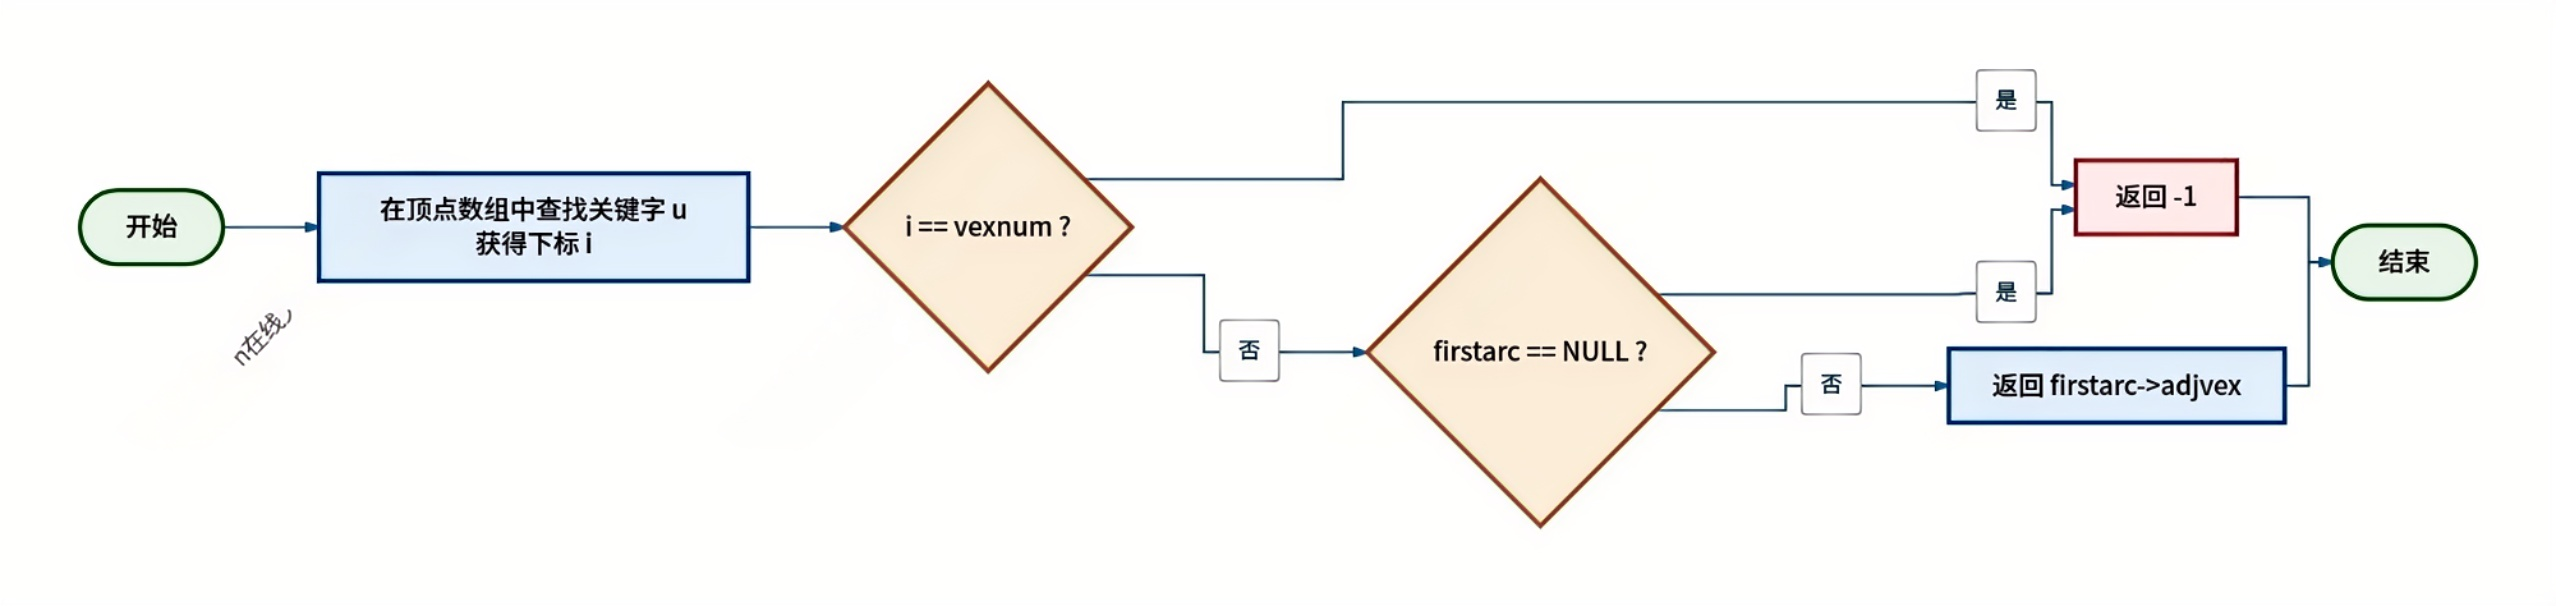
\includegraphics[width=\linewidth]{第一邻接点.png}
	\caption{第一邻接点}
\end{figure}
\begin{lstlisting}[label={lst:first-adj}, caption={FirstAdjVex}]
int FirstAdjVex(ALGraph G, KeyType u) {
    int i;
    for (i = 0; i < G.vexnum; i++)
        if (G.vertices[i].data.key == u) break;
    if (i == G.vexnum) return -1;
    if (G.vertices[i].firstarc == NULL) return -1;
    return G.vertices[i].firstarc->adjvex;
}
\end{lstlisting}

\subsubsection{NextAdjVex(G, v, w)——获得下一邻接点}
% Mermaid 参考: 图32 (NextAdjVex) — 见 Mermaid流程图.txt

\begin{quote}\small
\textbf{初始条件：}图G存在，v和w是G中两个顶点的关键字，w是v的邻接顶点。\\
\textbf{操作结果：}返回v的（相对于w）下一个邻接顶点的位序；若w是最后一个邻接顶点，返回-1。
\end{quote}

实现分析：先在v的弧链表中定位到w对应的ArcNode（遍历至adjvex等于w的下标），然后返回该ArcNode后继的adjvex。这是DFS/BFS遍历中"继续寻找下一个未访问邻接点"的核心操作。时间$O(n+e)$（需要先定位v和w，再遍历弧链）。
\begin{figure}[htb]
	\centering
	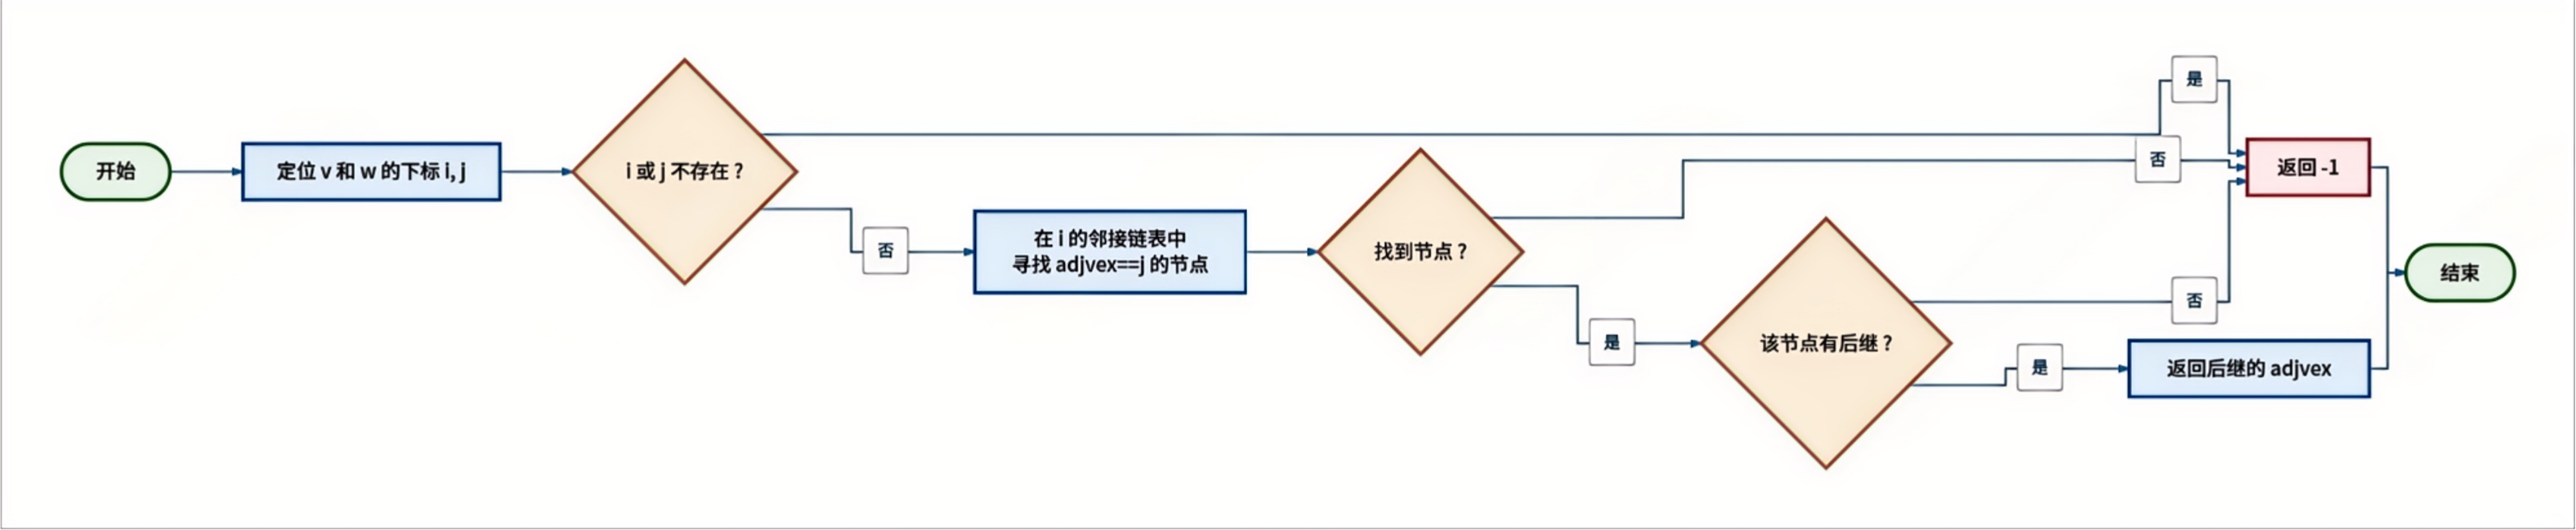
\includegraphics[width=\linewidth]{下一邻接点 (2).png}
	\caption{下一邻接点}
\end{figure}
\begin{lstlisting}[label={lst:next-adj}, caption={NextAdjVex}]
int NextAdjVex(ALGraph G, KeyType v, KeyType w) {
    int i, j;
    for (i = 0; i < G.vexnum; i++)
        if (G.vertices[i].data.key == v) break;
    for (j = 0; j < G.vexnum; j++)
        if (G.vertices[j].data.key == w) break;
    if (i == G.vexnum || j == G.vexnum) return -1;
    ArcNode *p = G.vertices[i].firstarc;
    while (p != NULL && p->adjvex != j) p = p->nextarc;
    if (p != NULL && p->nextarc != NULL) return p->nextarc->adjvex;
    return -1;
}
\end{lstlisting}

\subsubsection{InsertVex(G, v)——插入顶点}
% Mermaid 参考: 图33 (InsertVex) — 见 Mermaid流程图.txt

\begin{quote}\small
\textbf{初始条件：}图G存在，v和G中的顶点具有相同特征。\\
\textbf{操作结果：}在图G中增加新顶点v（保持关键字唯一性）。
\end{quote}

实现分析：检查容量和关键字唯一性后，在vertices数组末尾追加新顶点，初始化其firstarc为NULL。注意\textbf{新顶点是一个没有任何邻接边的孤立顶点}。时间$O(n)$（唯一性检查）。

\begin{lstlisting}[label={lst:insert-vex}, caption={InsertVex}]
status InsertVex(ALGraph *G, VertexType v) {
    if (G->vexnum >= MAX_VERTEX_NUM) return ERROR;
    for (int i = 0; i < G->vexnum; i++)
        if (G->vertices[i].data.key == v.key) return ERROR;
    G->vertices[G->vexnum].data = v;
    G->vertices[G->vexnum].firstarc = NULL;
    G->vexnum++;
    return OK;
}
\end{lstlisting}

\subsubsection{DeleteVex(G, v)——删除顶点}
% Mermaid 参考: 图34 (DeleteVex 四步删除) — 见 Mermaid流程图.txt

\begin{quote}\small
\textbf{初始条件：}图G存在，v是和G中顶点关键字类型相同的给定值。\\
\textbf{操作结果：}删除关键字v对应的顶点以及所有与之相关的弧。
\end{quote}

实现分析：\textbf{邻接表中最复杂的操作}，需四步紧密协作，缺一不可。


\begin{lstlisting}[label={lst:delete-vex}, caption={DeleteVex——最复杂的邻接表操作}]
status DeleteVex(ALGraph *G, KeyType v) {
    int i, j, m = 0;
    for (i = 0; i < G->vexnum; i++)
        if (G->vertices[i].data.key == v) break;
    if (i == G->vexnum || G->vexnum == 1) return ERROR;
    ArcNode *p = G->vertices[i].firstarc;
    while (p) { m++; p = p->nextarc; }            // 步骤1
    for (j = 0; j < G->vexnum; j++) {             // 步骤2
        if (j == i) continue;
        ArcNode *pre = NULL; p = G->vertices[j].firstarc;
        while (p) {
            if (p->adjvex == i) {
                if (pre == NULL) G->vertices[j].firstarc = p->nextarc;
                else pre->nextarc = p->nextarc;
                ArcNode *q = p; p = p->nextarc; free(q);
            } else { pre = p; p = p->nextarc; }
        }
    }
    p = G->vertices[i].firstarc;                   // 步骤3
    while (p) { ArcNode *q = p; p = p->nextarc; free(q); }
    for (j = i + 1; j < G->vexnum; j++)            // 步骤4
        G->vertices[j - 1] = G->vertices[j];
    G->vexnum--;
    for (j = 0; j < G->vexnum; j++) {
        p = G->vertices[j].firstarc;
        while (p) { if (p->adjvex > i) p->adjvex--; p = p->nextarc; }
    }
    G->arcnum -= m;
    return OK;
}
\end{lstlisting}

\begin{figure}[H]
\centering\footnotesize
\resizebox{\textwidth}{!}{
\begin{tikzpicture}[node distance=0.45cm, flowStart, flowProc, flowDec, flowArr]
\node (start) [flowStart] {DeleteVex 入口};
\node (find) [flowProc, below=of start] {定位被删顶点下标i\\（LocateVex）};
\node (chk) [flowDec, below=of find] {顶点存在且\\vexnum>1?};
\node (bad) [flowStart, right=3.0cm of chk, fill=orange!30] {返回 ERROR};

% Four steps
\node (s1) [flowProc, below=of chk] {\textbf{步骤1} 统计关联弧数m\\遍历firstarc[i]计数};
\node (s2) [flowProc, below=of s1] {\textbf{步骤2} 清理引用弧\\删除其他顶点链表中\\adjvex==i的ArcNode\\（区分头删/中间删）};
\node (s3) [flowProc, below=of s2] {\textbf{步骤3} 释放自身弧链表\\释放顶点i的全部ArcNode};
\node (s4) [flowProc, below=of s3] {\textbf{步骤4} 数组前移+下标校正\\① vertices[i..vexnum-2]前移1位\\② 全局扫描adjvex>i的减1};
\node (upd) [flowProc, below=of s4] {G->vexnum--; G->arcnum-=m};
\node (ok) [flowStart, below=of upd, fill=green!30] {返回 OK};

\draw [flowArr] (start) -- (find) -- (chk);
\draw [flowArr] (chk.east) -- node[above]{否} (bad.west);
\draw [flowArr] (chk) -- node[right]{是} (s1);
\draw [flowArr] (s1) -- (s2);
\draw [flowArr] (s2) -- (s3);
\draw [flowArr] (s3) -- (s4);
\draw [flowArr] (s4) -- (upd);
\draw [flowArr] (upd) -- (ok);

% Right annotation
\node [right=2.0cm of s2, text width=4.2cm, align=left, font=\tiny, draw=gray, dashed, inner sep=3pt] {
    \textbf{步骤4下标校正原理:}\\
    删除顶点i后，原下标>i的\\
    顶点都前移了1位，因此所有\\
    ArcNode中adjvex>i的值\\
    必须减1，否则将指向错误\\
    的顶点。\\[2pt]
    例：原adjvex=5(指向vertices[5])\\
    ~~删除i=3后，原vertices[5]\\
    ~~变为vertices[4]，故adjvex\\
% Mermaid 参考: 图34 (DeleteVex四步删除) — 见 Mermaid流程图.txt
    ~~需从5减为4。
};
\end{tikzpicture}
}
\caption{DeleteVex四步删除流程图}
\label{fig:deletevex-flow}
\end{figure}
\subsubsection{InsertArc(G, v, w)——插入弧}
% Mermaid 参考: 图35 (InsertArc) — 见 Mermaid流程图.txt

\begin{quote}\small
\textbf{初始条件：}图G存在，v、w是和G中顶点关键字类型相同的给定值。\\
\textbf{操作结果：}在图G中增加弧<v,w>；由于G是无向图，还需增加<w,v>。
\end{quote}

实现分析：检查三点有效性——顶点存在、非自环、边不存在。通过后创建两个ArcNode头插到两个顶点的弧链表头部。时间$O(n+e)$。


\begin{lstlisting}[label={lst:insert-arc}, caption={InsertArc}]
status InsertArc(ALGraph *G, KeyType v, KeyType w) {
    int i, j;
    for (i = 0; i < G->vexnum; i++)
        if (G->vertices[i].data.key == v) break;
    for (j = 0; j < G->vexnum; j++)
        if (G->vertices[j].data.key == w) break;
    if (i == G->vexnum || j == G->vexnum || i == j) return ERROR;
    ArcNode *p = G->vertices[i].firstarc;
    while (p) { if (p->adjvex == j) return ERROR; p = p->nextarc; }
    ArcNode *n1 = (ArcNode*)malloc(sizeof(ArcNode));
    n1->adjvex = j; n1->nextarc = G->vertices[i].firstarc;
    G->vertices[i].firstarc = n1;
    ArcNode *n2 = (ArcNode*)malloc(sizeof(ArcNode));
    n2->adjvex = i; n2->nextarc = G->vertices[j].firstarc;
    G->vertices[j].firstarc = n2;
    G->arcnum++;
    return OK;
}
\end{lstlisting}

\subsubsection{DeleteArc(G, v, w)——删除弧}
% Mermaid 参考: 图36 (DeleteArc) — 见 Mermaid流程图.txt

\begin{quote}\small
\textbf{初始条件：}图G存在，v、w是和G中顶点关键字类型相同的给定值。\\
\textbf{操作结果：}删除弧<v,w>；由于G是无向图，还需删除<w,v>。
\end{quote}

实现分析：需要从两个方向的弧链表中分别找到并删除对应ArcNode。每个方向的删除都需区分"删头节点"（修改firstarc）和"删中间节点"（修改前驱的nextarc）两种情况。时间$O(n+e)$。

\begin{lstlisting}[label={lst:delete-arc}, caption={DeleteArc}]
status DeleteArc(ALGraph *G, KeyType v, KeyType w) {
    int i, j;
    for (i = 0; i < G->vexnum; i++)
        if (G->vertices[i].data.key == v) break;
    for (j = 0; j < G->vexnum; j++)
        if (G->vertices[j].data.key == w) break;
    if (i == G->vexnum || j == G->vexnum || i == j) return ERROR;
    // 删除 v→w
    ArcNode *pre = NULL, *p = G->vertices[i].firstarc;
    while (p && p->adjvex != j) { pre = p; p = p->nextarc; }
    if (p == NULL) return ERROR;
    if (pre == NULL) G->vertices[i].firstarc = p->nextarc;
    else pre->nextarc = p->nextarc;
    free(p);
    // 删除 w→v
    pre = NULL; p = G->vertices[j].firstarc;
    while (p && p->adjvex != i) { pre = p; p = p->nextarc; }
    if (pre == NULL) G->vertices[j].firstarc = p->nextarc;
    else pre->nextarc = p->nextarc;
    free(p);
    G->arcnum--;
    return OK;
}
\end{lstlisting}
\begin{figure}[htb]
	\centering
	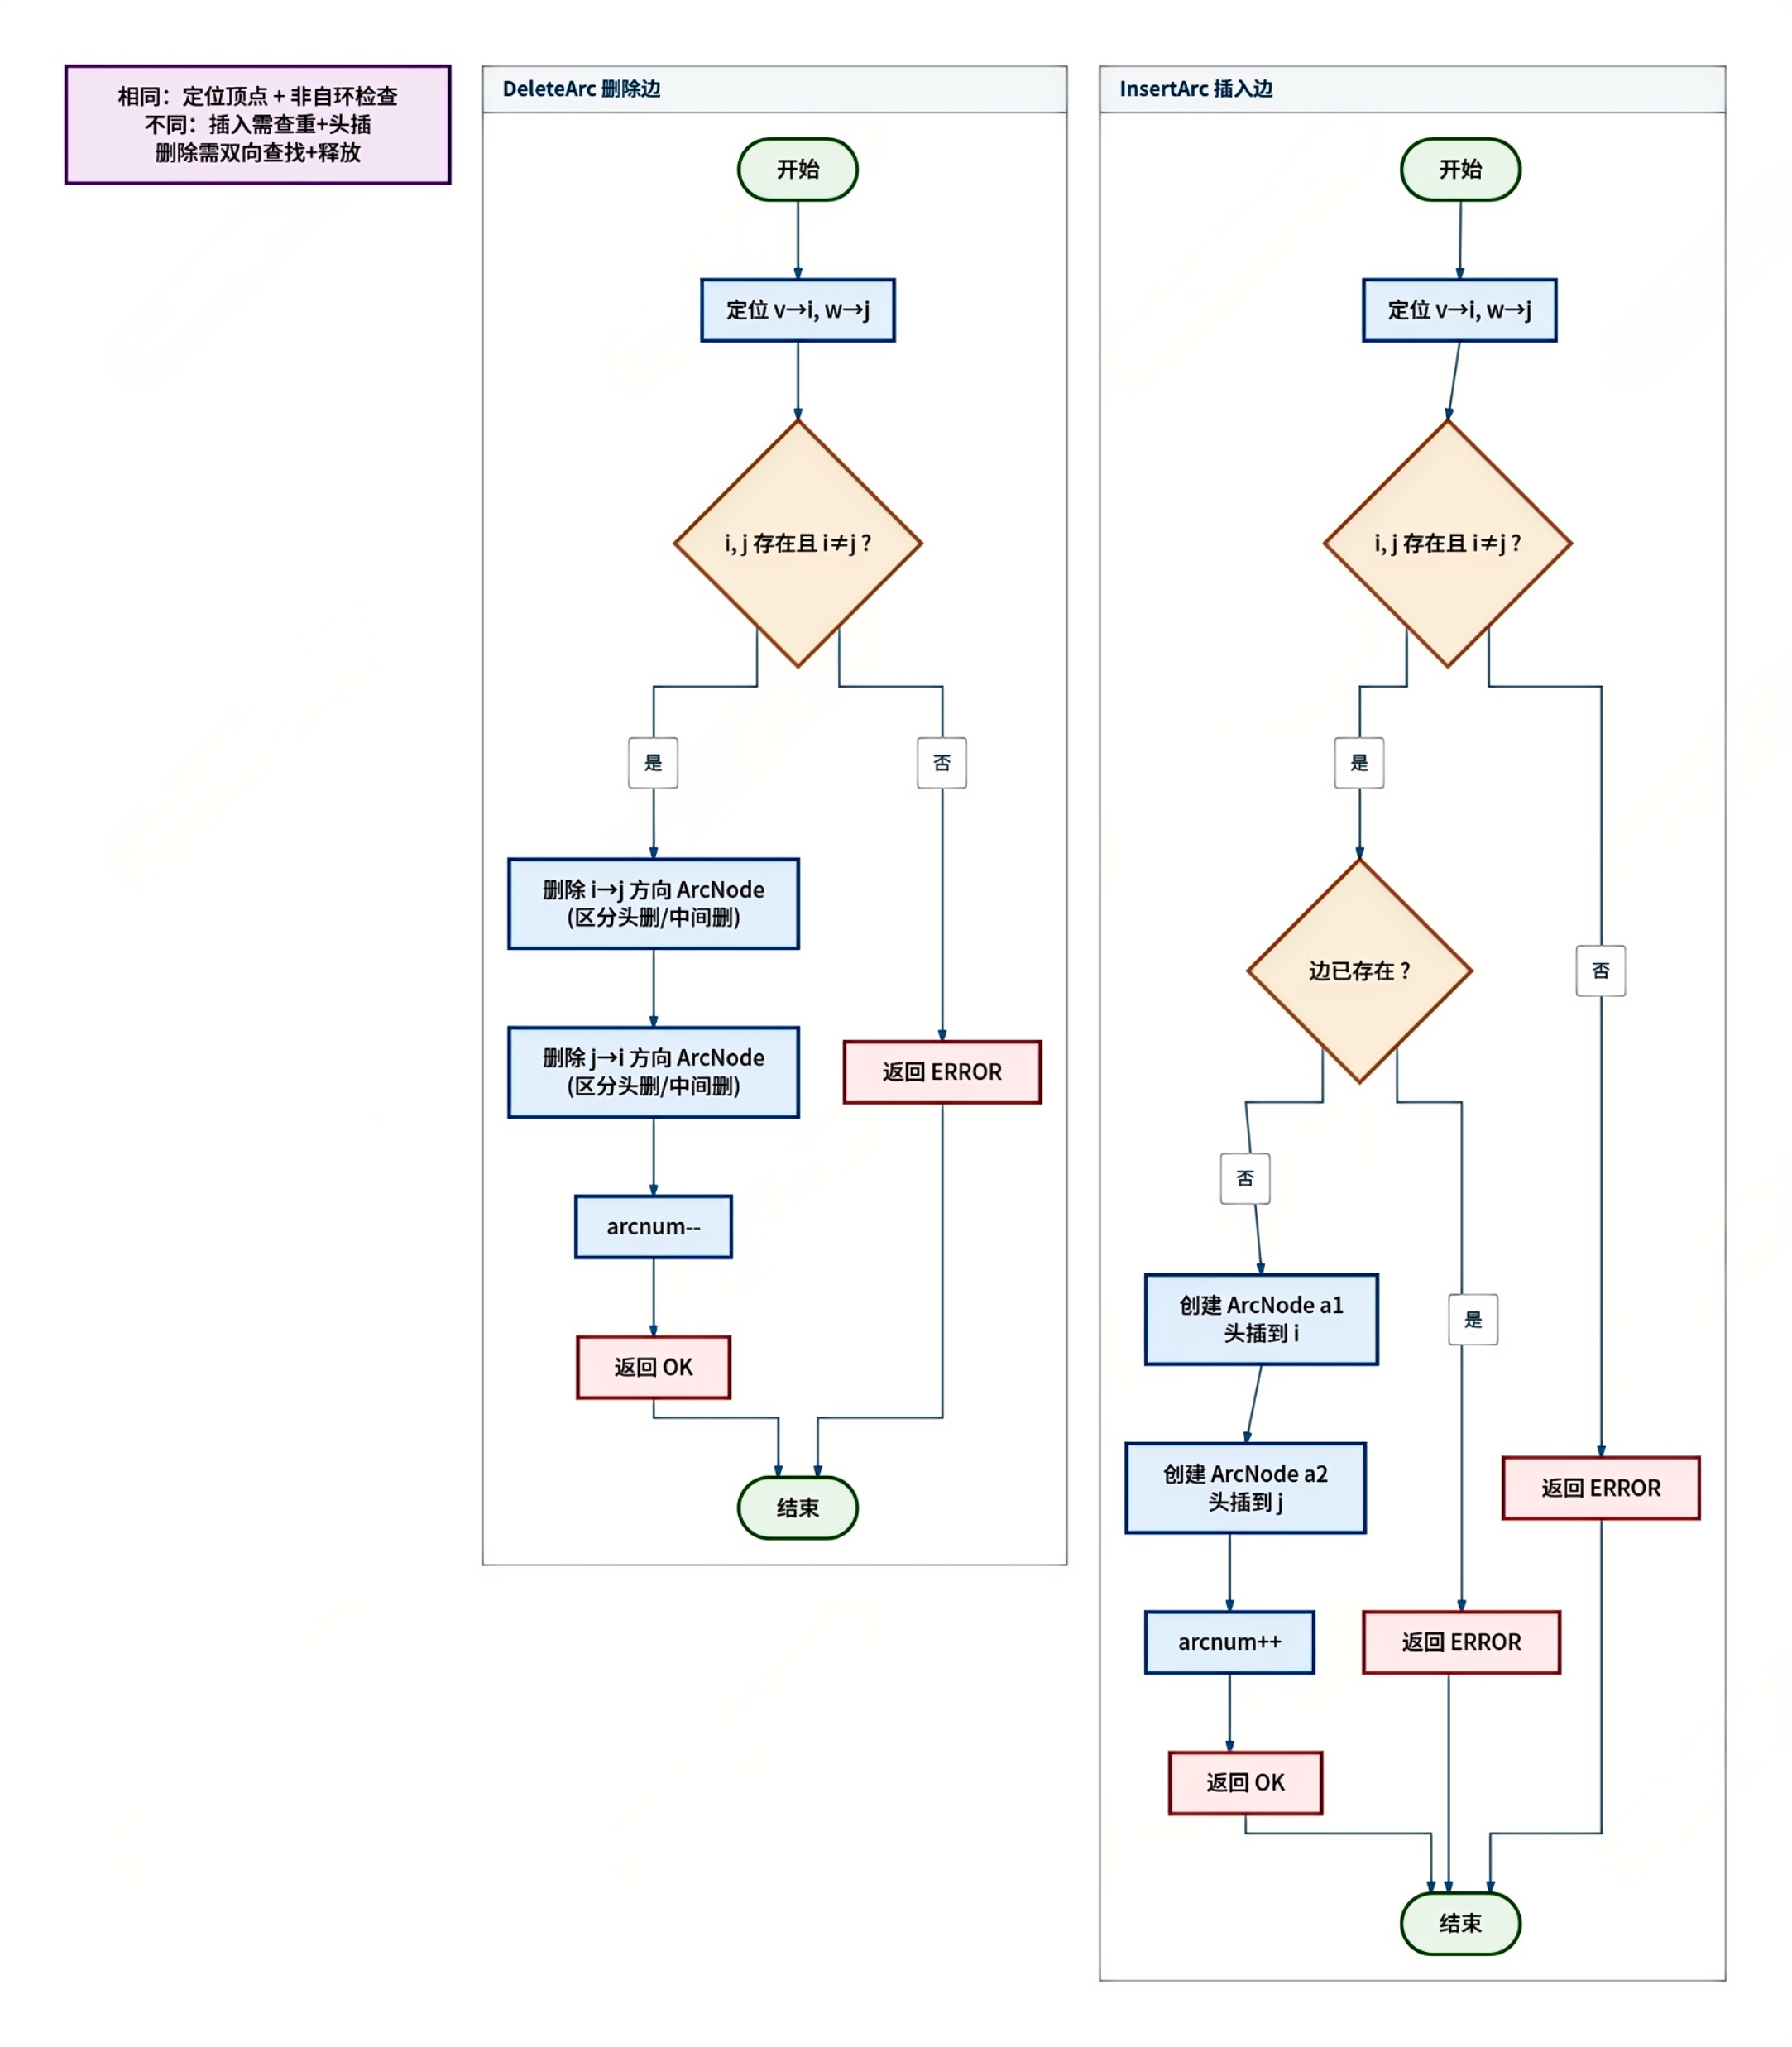
\includegraphics[width=0.85\linewidth]{插入边与删除边.png}
	\caption{插入弧与删除弧}
\end{figure}


\subsubsection{DFSTraverse(G, visit())——深度优先搜索遍历}
% Mermaid 参考: 图37 (DFSTraverse) — 见 Mermaid流程图.txt

\begin{quote}\small
\textbf{初始条件：}图G存在。\quad\textbf{操作结果：}对G进行深度优先搜索遍历，依次对每个顶点调用visit访问一次且仅一次。
\end{quote}

\textbf{算法设计：}采用\textbf{非递归栈实现}DFS（显式栈数组stack[]替代系统递归栈），以避免深度极大时的栈溢出。外层for循环确保非连通图的每个连通分量都被遍历。

DFS运作方式：访问起始顶点→入栈→循环查栈顶顶点的邻接边找第一个未访问邻接点→找到则访问并入栈（深入）；找不到则弹栈（回溯）。
\newpage
\begin{figure}[H]
	\centering
	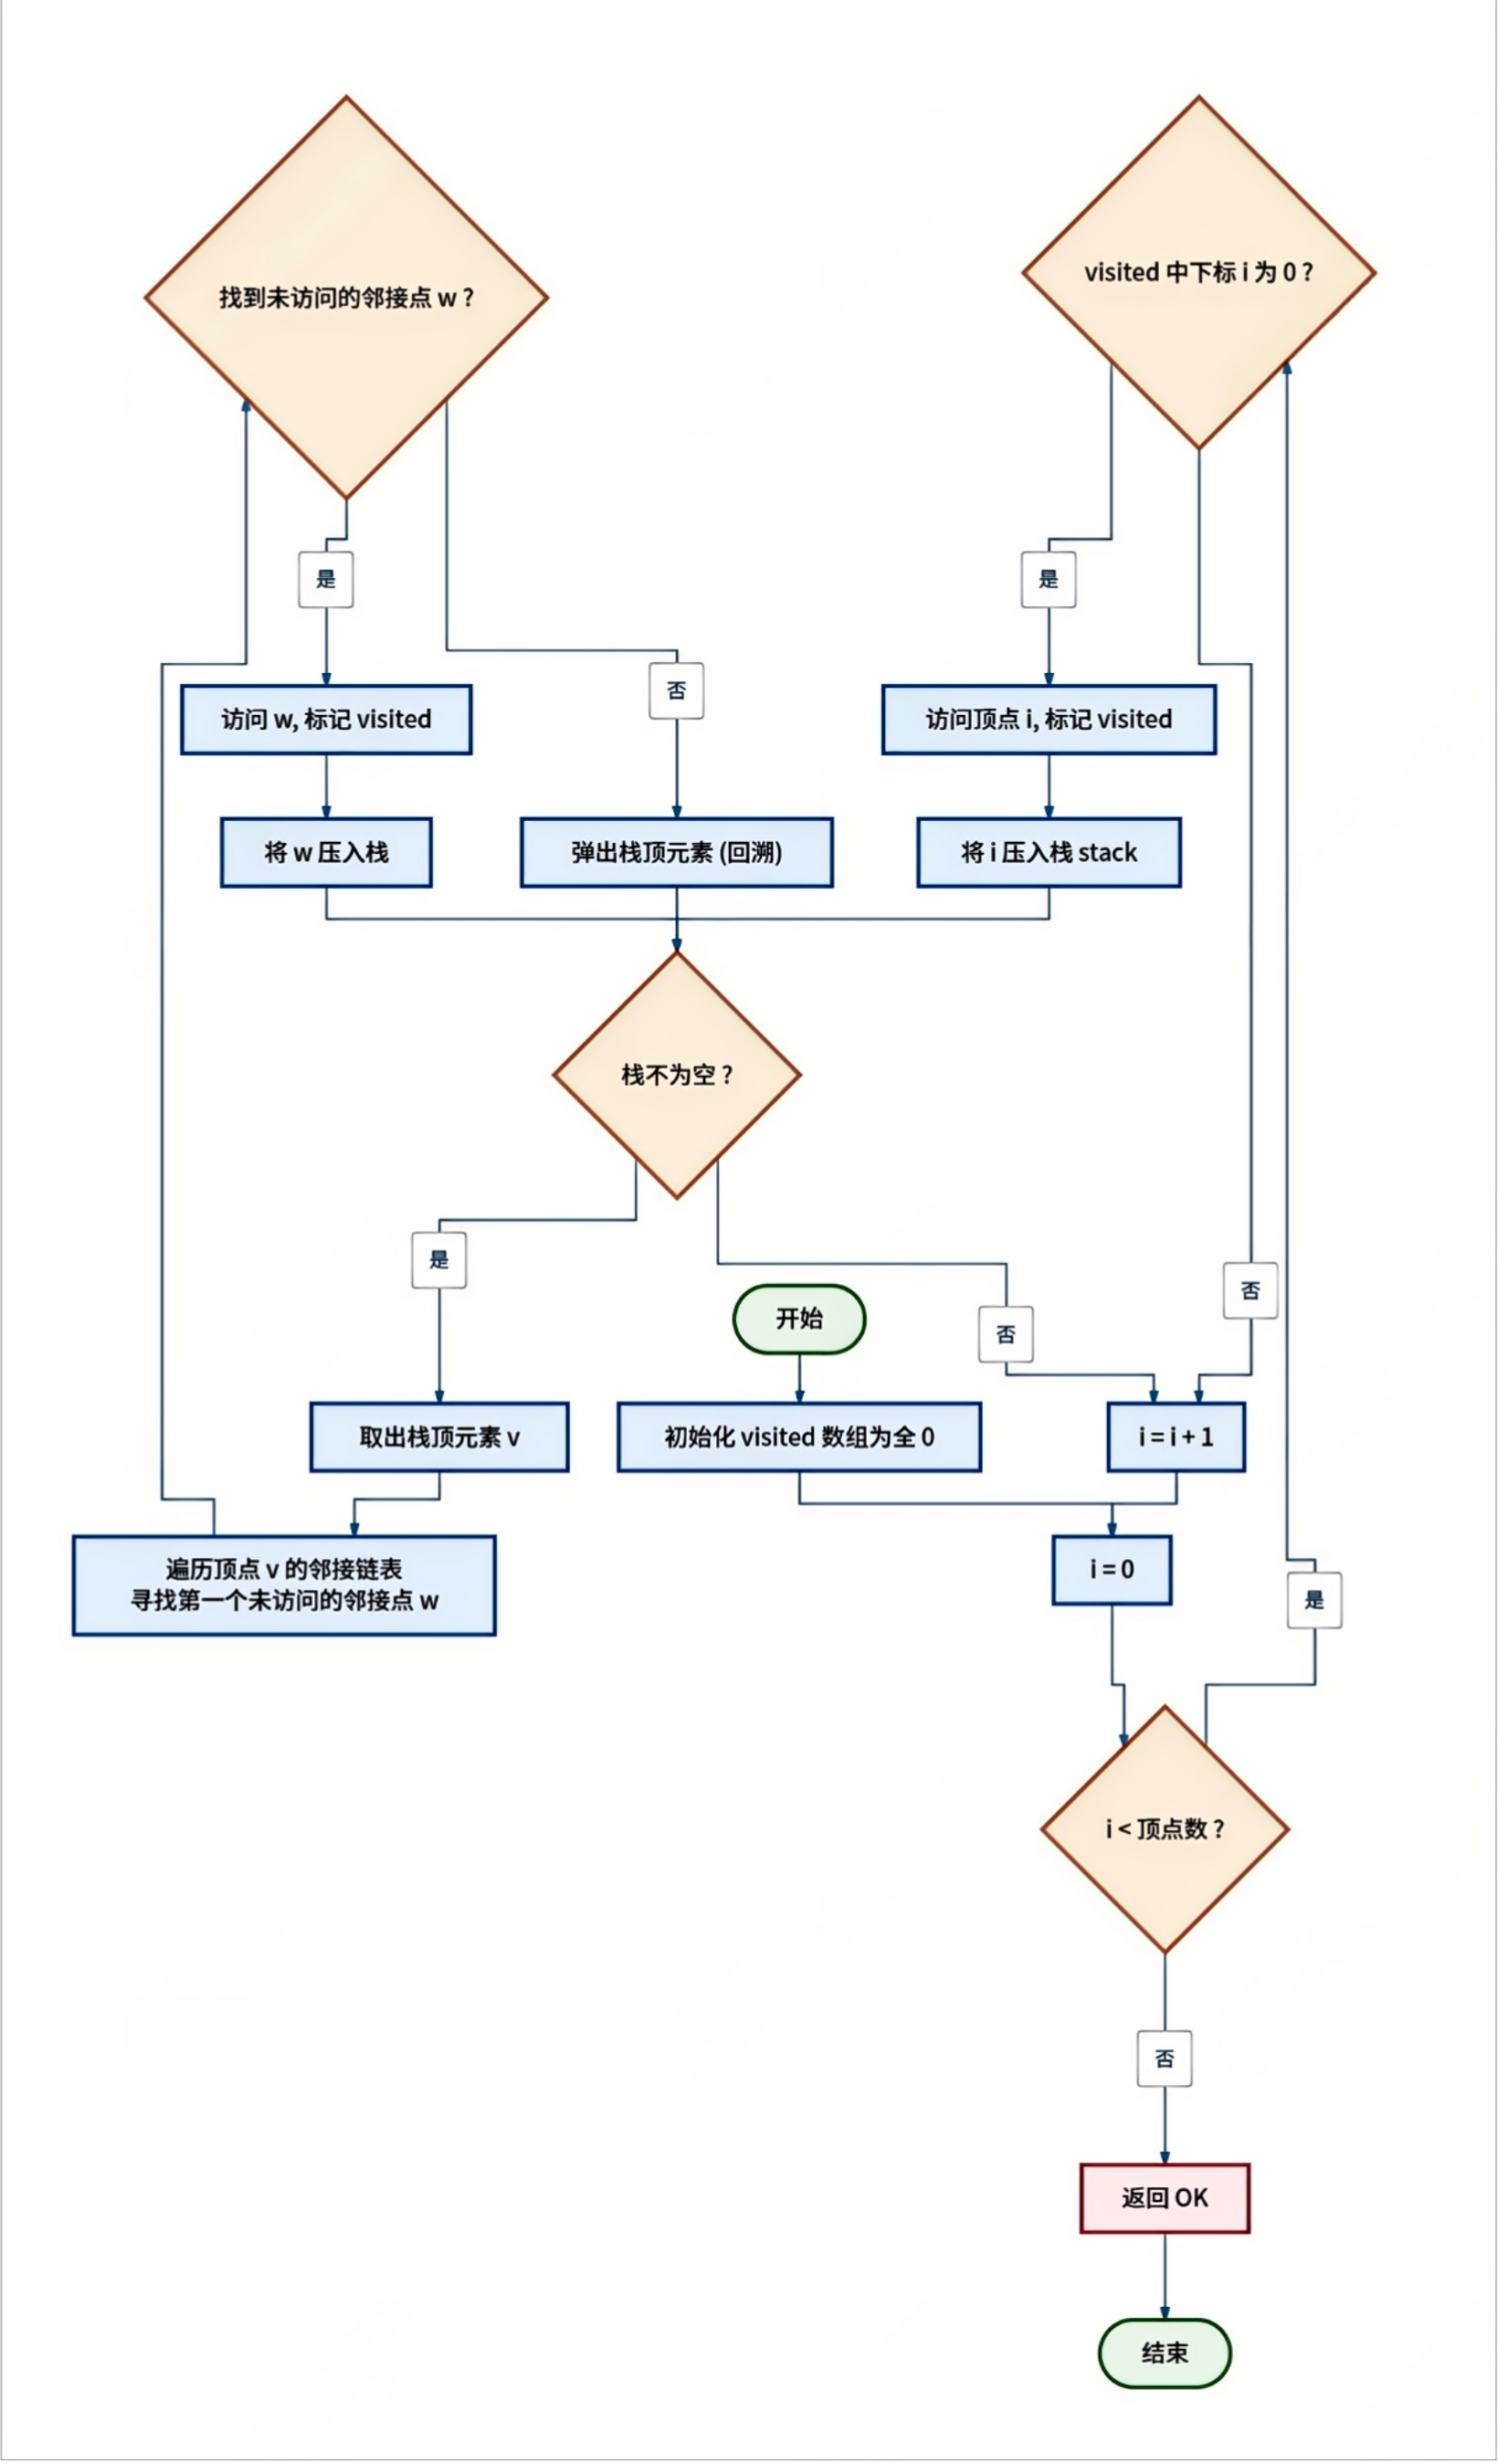
\includegraphics[width=0.6\linewidth]{DFS.png}
	\caption{DFS算法流程示意图}
\end{figure}
\begin{figure}[H]
	\centering
	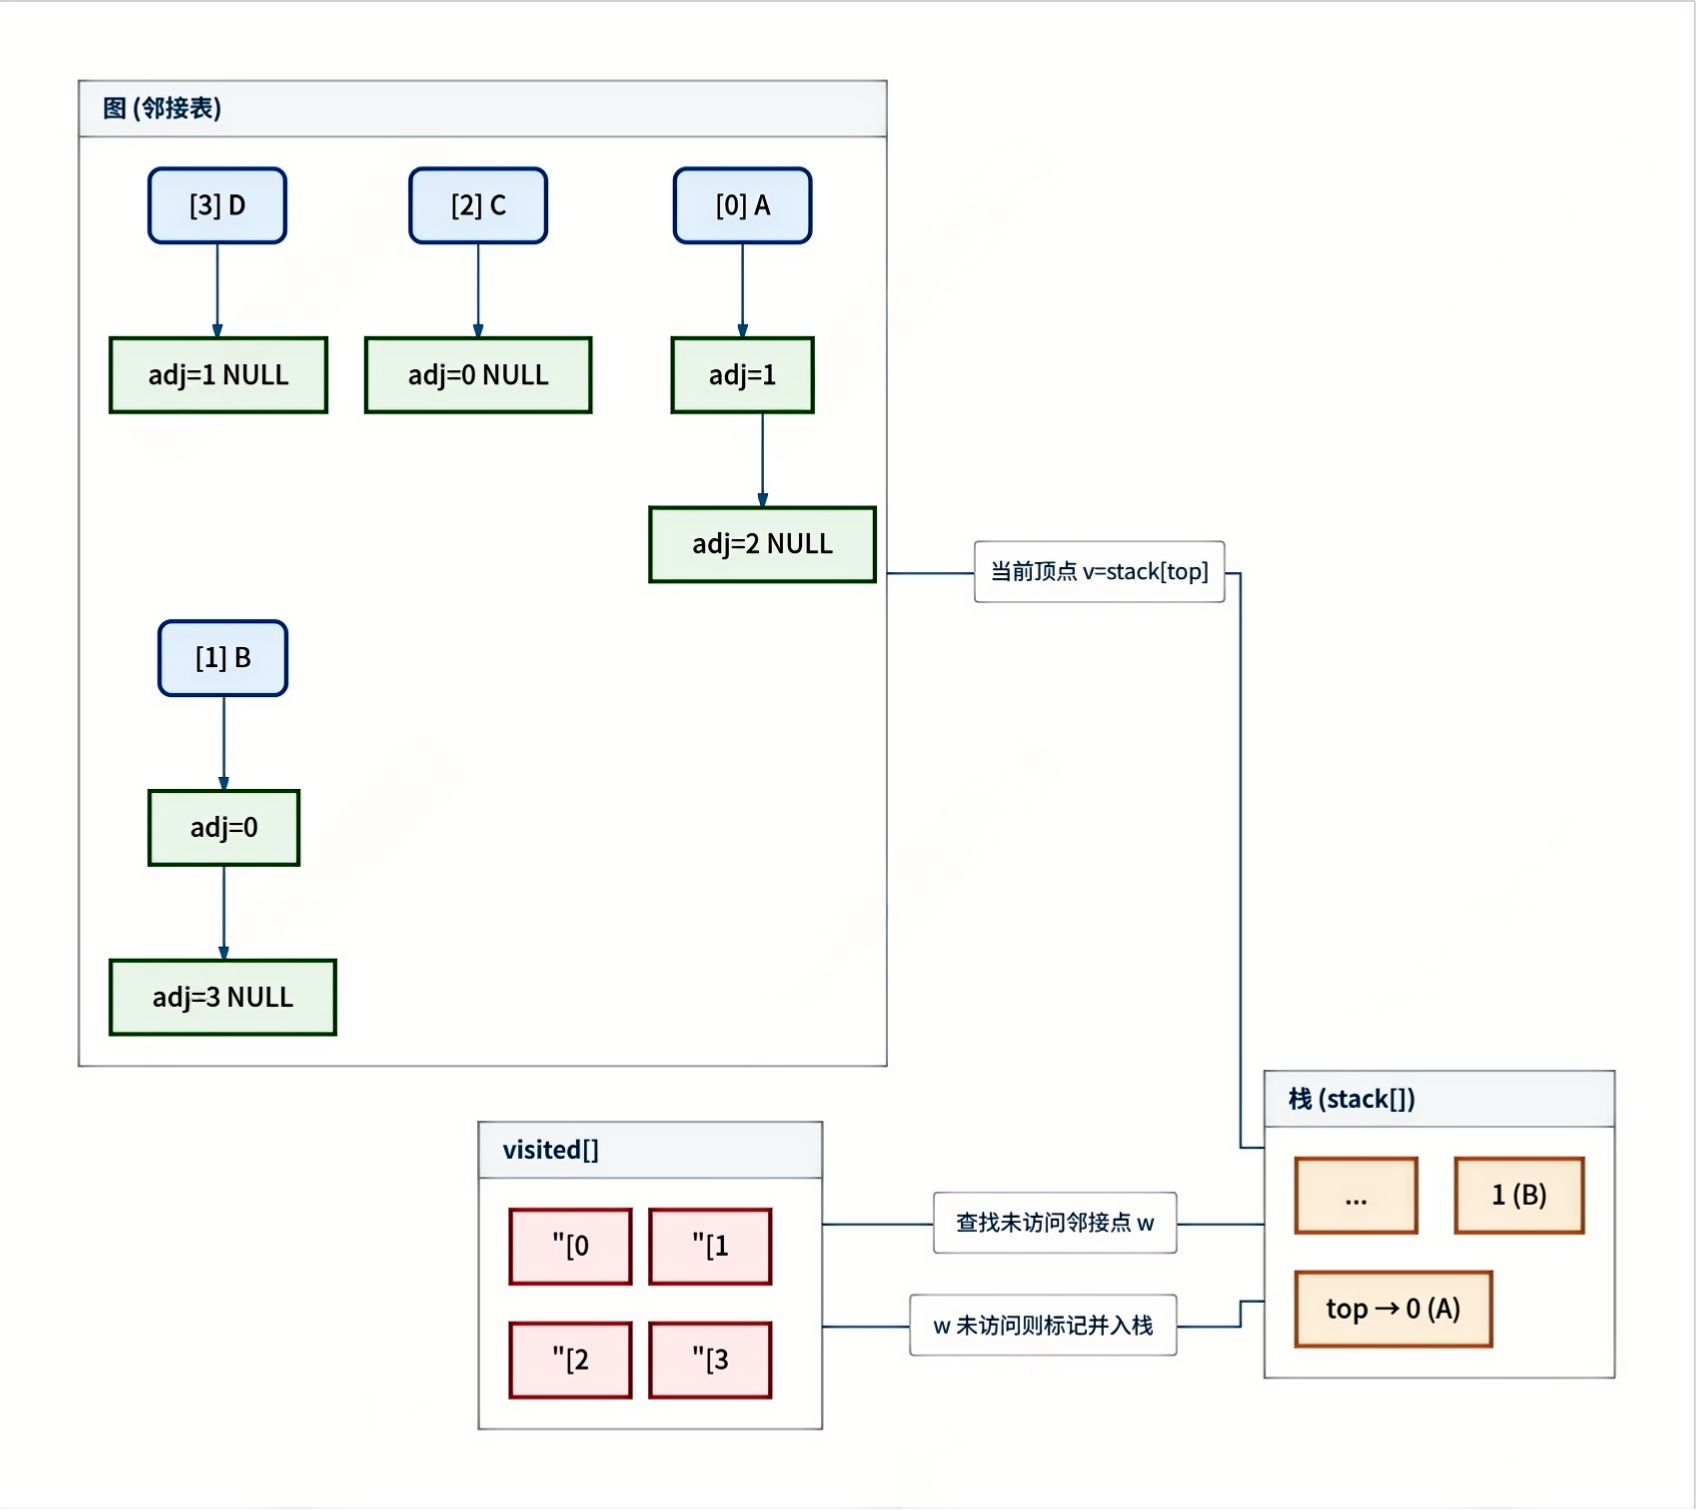
\includegraphics[width=0.5\linewidth]{DFS结构.png}
	\caption{DFS数据结构示意图}
\end{figure}
\newpage
\begin{lstlisting}[label={lst:dfs}, caption={DFSTraverse——非递归栈实现}]
status DFSTraverse(ALGraph *G, void (*visit)(VertexType)) {
    int visited[MAX_VERTEX_NUM];
    for (int i = 0; i < G->vexnum; i++) visited[i] = 0;
    for (int i = 0; i < G->vexnum; i++) {
        if (!visited[i]) {
            int stack[MAX_VERTEX_NUM], top = -1;
            visited[i] = 1; visit(G->vertices[i].data);
            stack[++top] = i;
            while (top >= 0) {
                int v = stack[top];
                ArcNode *p = G->vertices[v].firstarc;
                int w = -1;
                while (p != NULL) {
                    if (!visited[p->adjvex]) { w = p->adjvex; break; }
                    p = p->nextarc;
                }
                if (w != -1) {
                    visited[w] = 1; visit(G->vertices[w].data);
                    stack[++top] = w;
                } else { top--; }
            }
        }
    }
    return OK;
}
\end{lstlisting}

\textbf{算法分析：}时间$O(n+e)$（每个顶点和弧恰好访问一次）；空间$O(n)$（visited数组+栈）。非递归DFS的栈深度在最坏情况（图为一条链）下等于n。外层for循环+visited数组共同保证了非连通图的每个连通分量都被遍历。

\subsubsection{BFSTraverse(G, visit())——广度优先搜索遍历}
% Mermaid 参考: 图38 (BFSTraverse) — 见 Mermaid流程图.txt

\begin{quote}\small
\textbf{初始条件：}图G存在。\quad\textbf{操作结果：}对G进行广度优先搜索遍历，依次对每个顶点调用visit访问一次且仅一次。
\end{quote}

\textbf{算法设计：}使用\textbf{队列}实现BFS。访问一个顶点后将其所有未访问邻接点全部加入队列，使得访问顺序按"距起始顶点0步→1步→2步→..."逐层展开。这种层次遍历特性是BFS能解决最短路径问题的理论基础。流程图见下页：

\newpage
\begin{figure}[H]
	\centering
	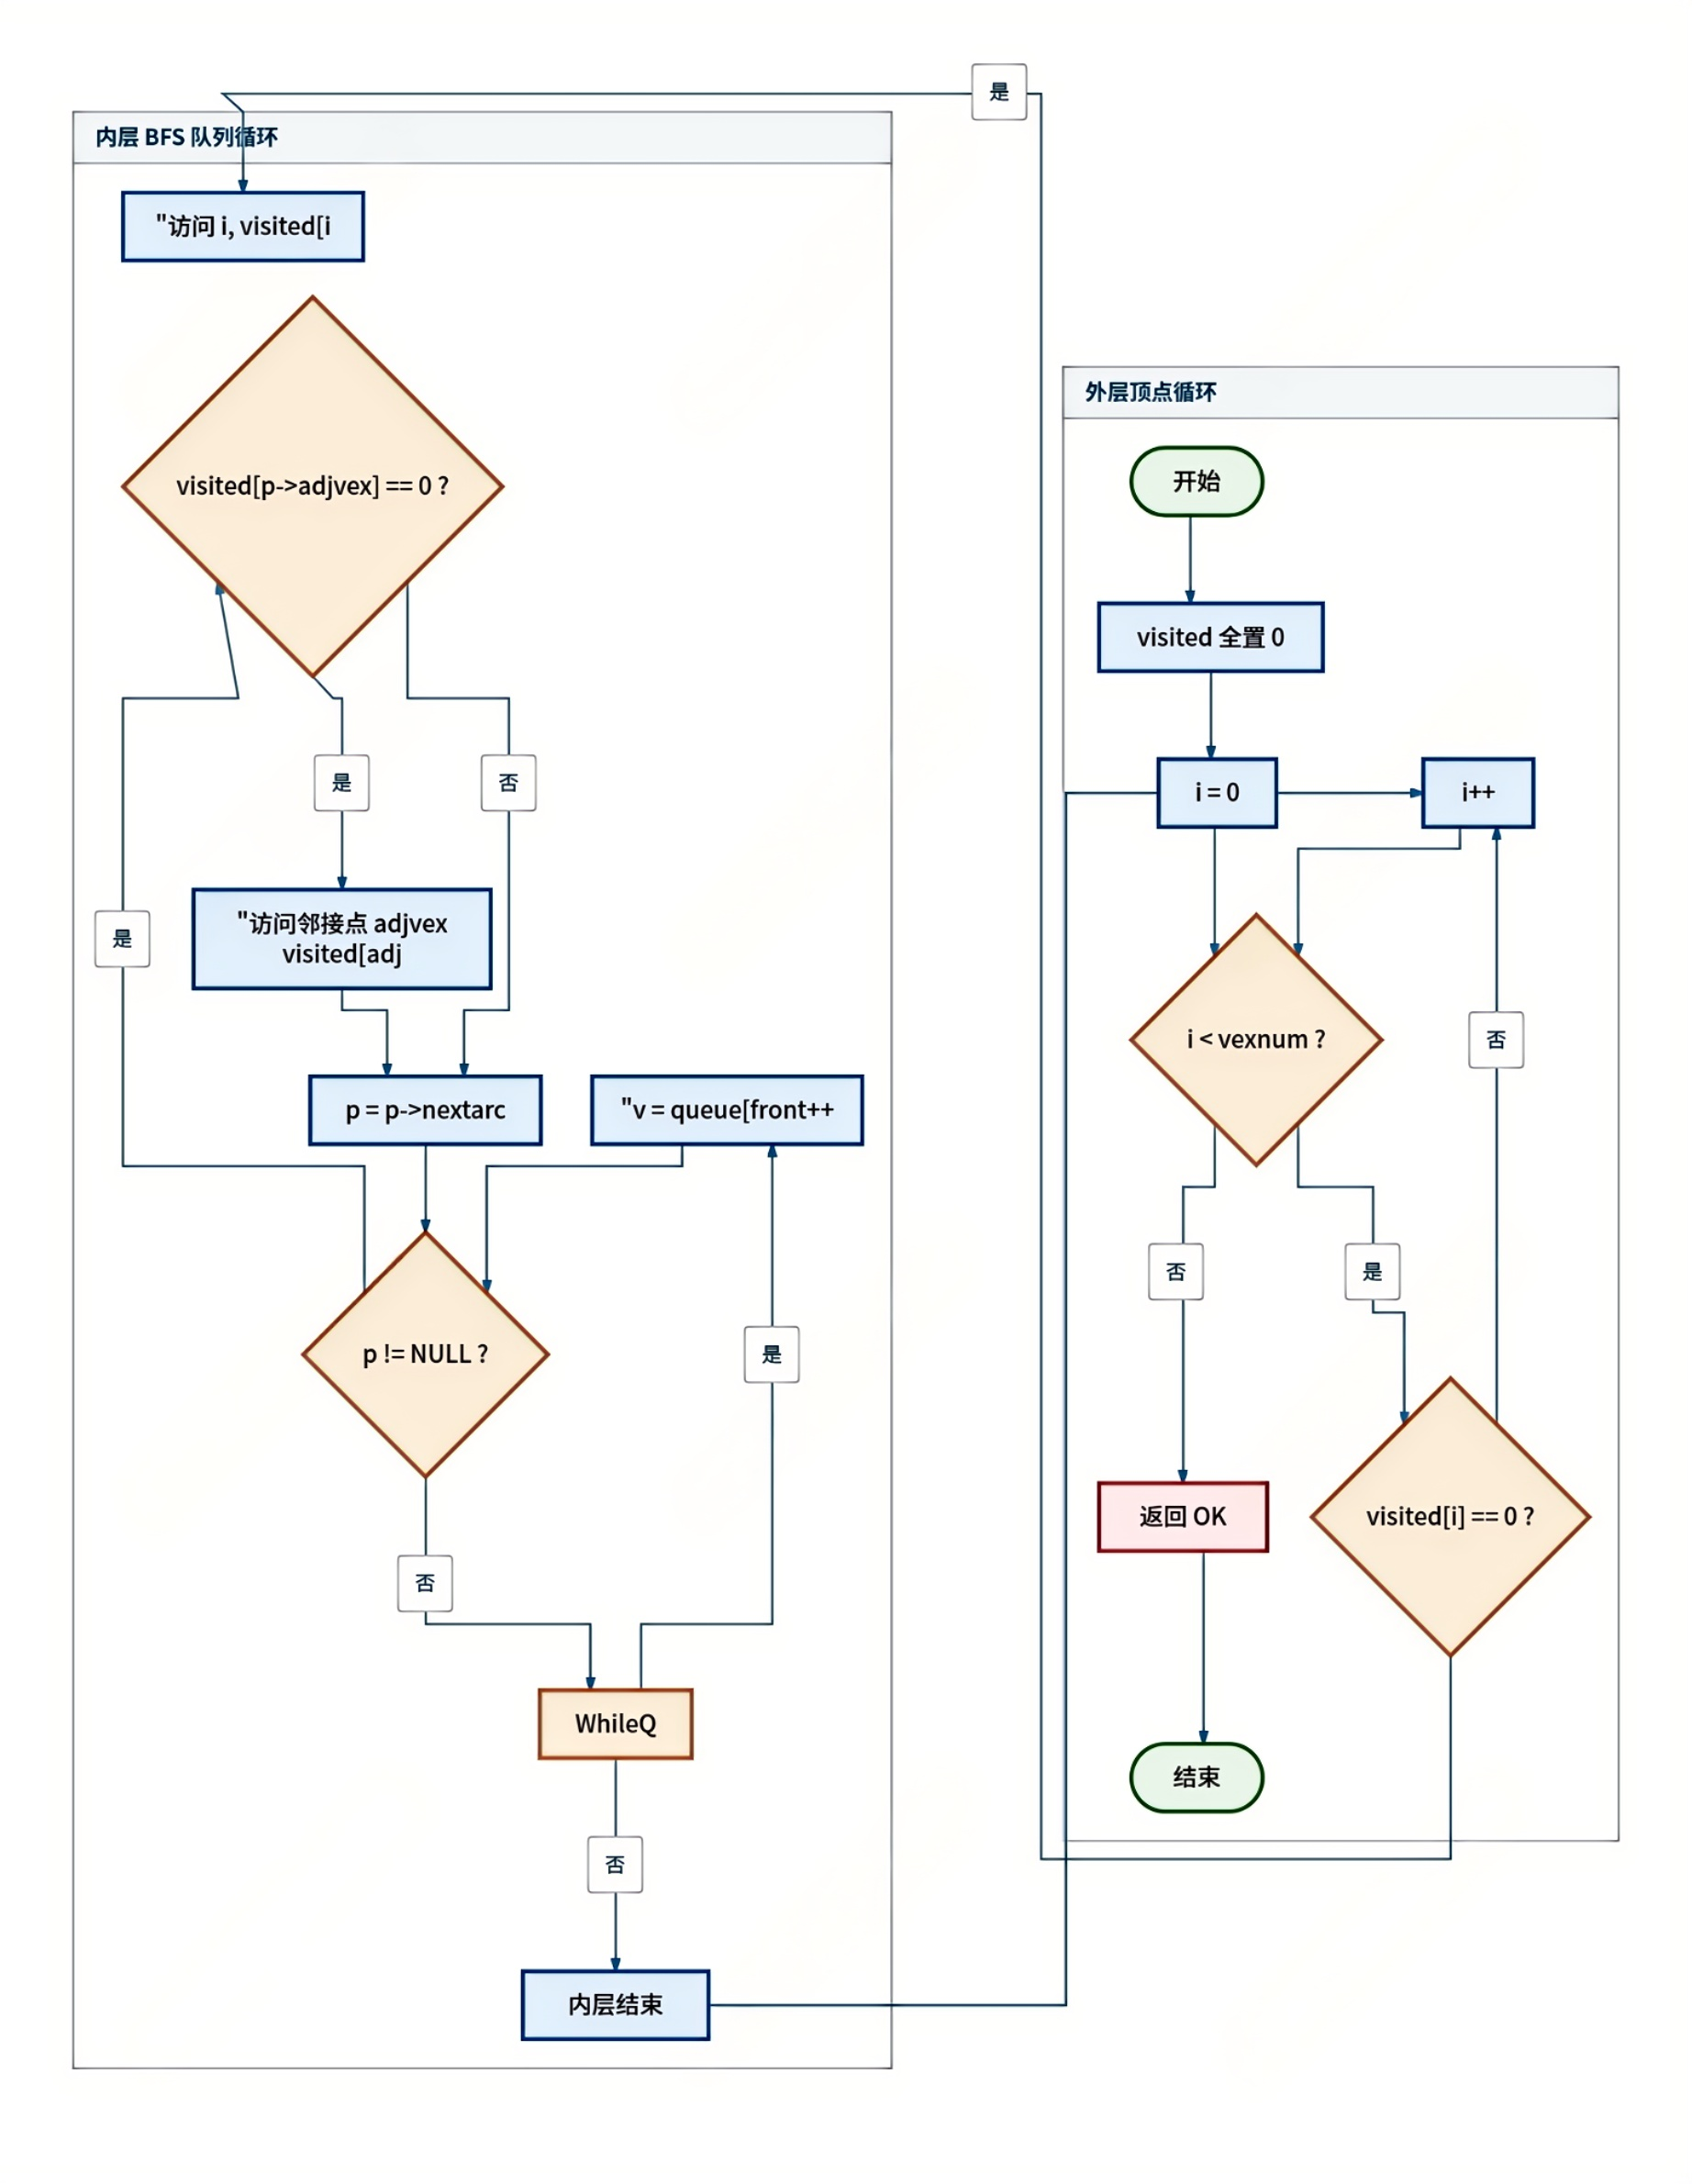
\includegraphics[width=0.85\linewidth]{BFS (2).png}
    \caption{BFS流程图}
\end{figure}
\begin{figure}[H]
	\centering
	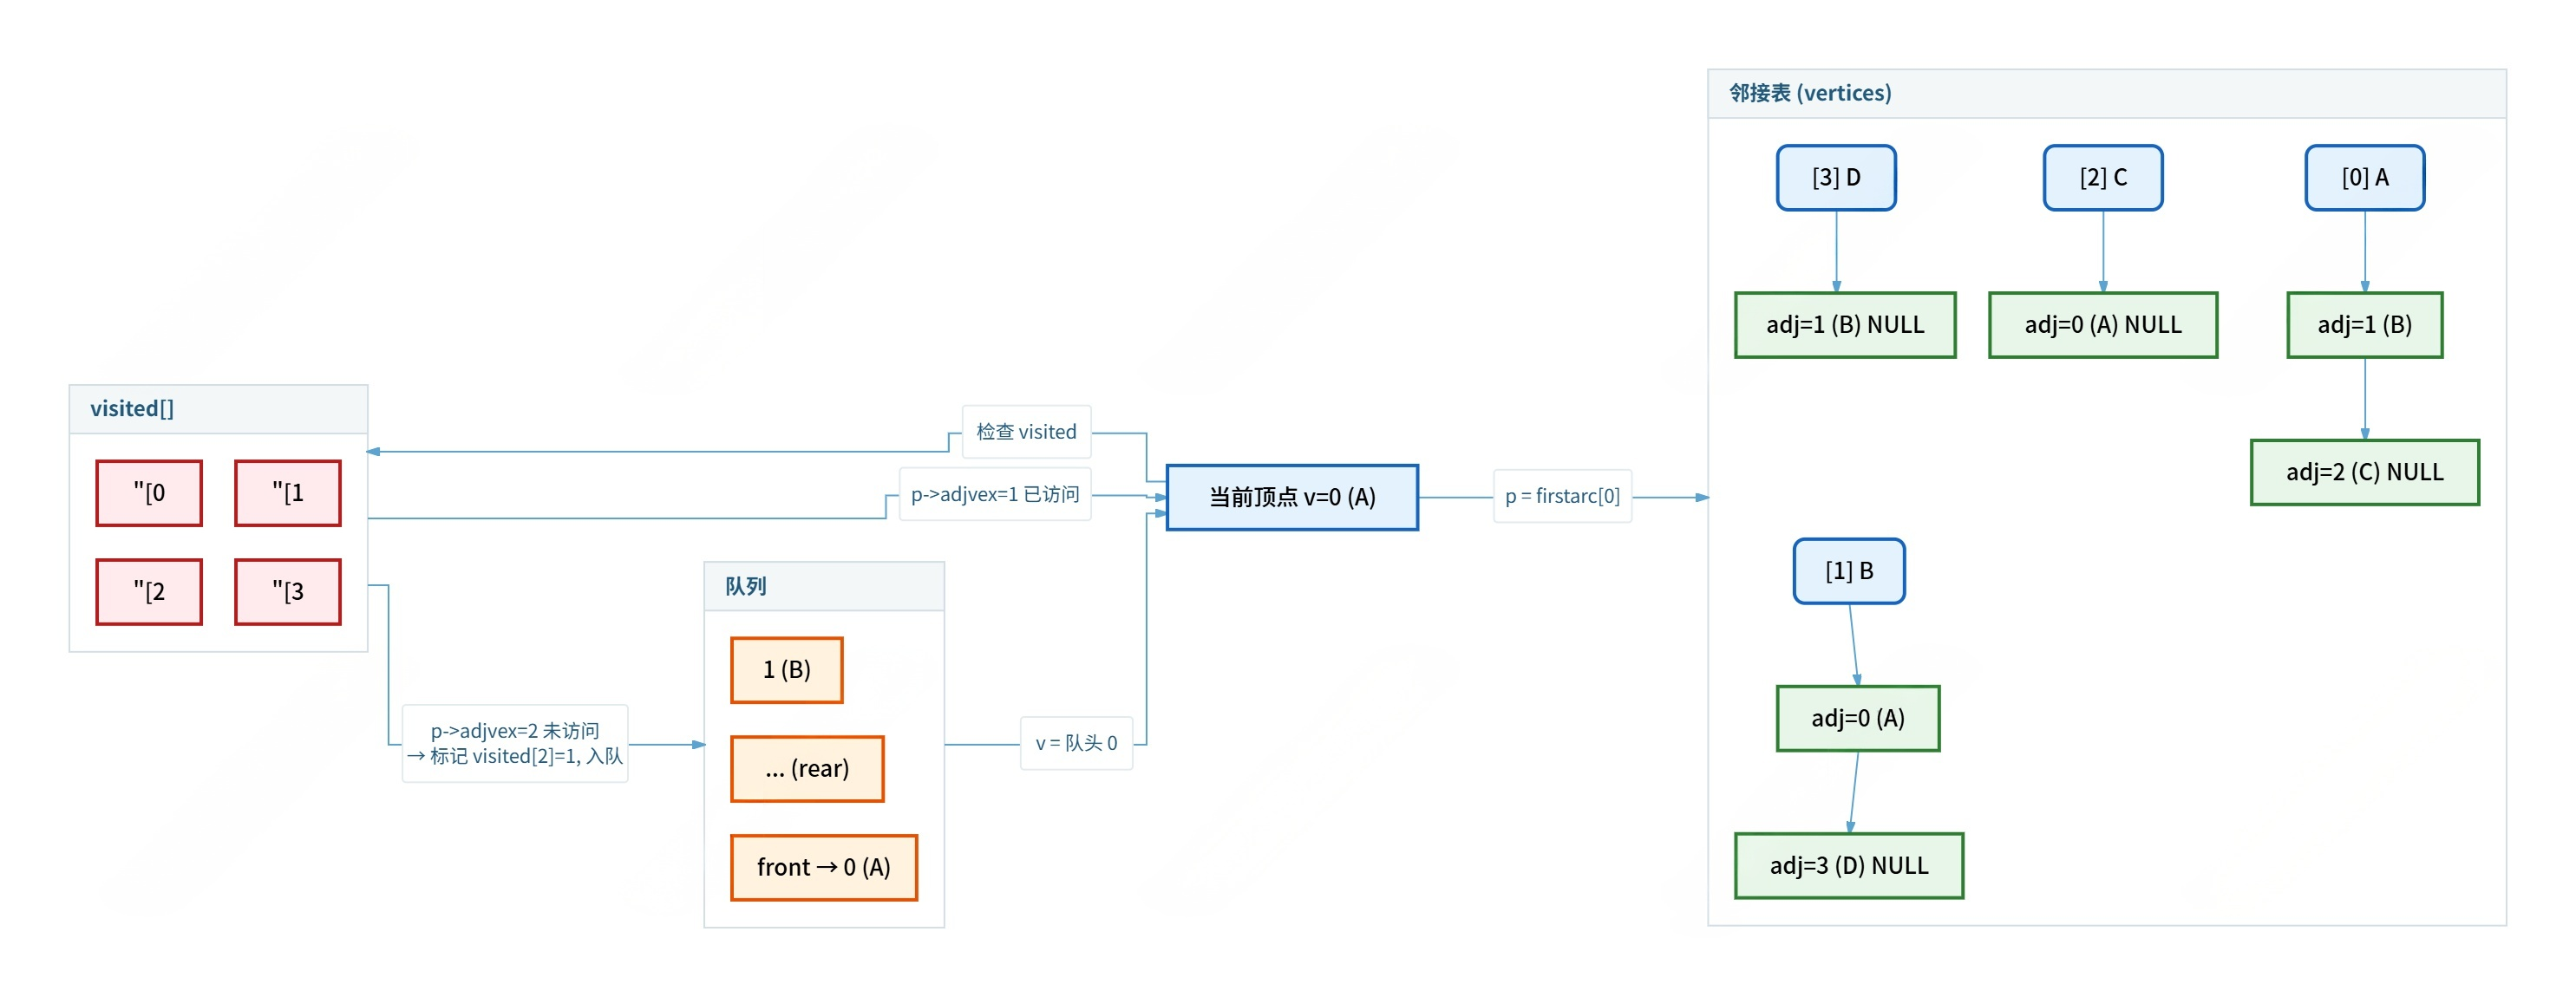
\includegraphics[width=\linewidth]{BFS数据结构.png}
	\caption{BFS结构示意图}
\end{figure}
\newpage

\begin{lstlisting}[label={lst:bfs}, caption={BFSTraverse——队列实现}]
status BFSTraverse(ALGraph *G, void (*visit)(VertexType)) {
    int visited[MAX_VERTEX_NUM];
    int queue[MAX_VERTEX_NUM], front, rear;
    for (int i = 0; i < G->vexnum; i++) visited[i] = 0;
    for (int i = 0; i < G->vexnum; i++) {
        if (!visited[i]) {
            front = rear = 0;
            visited[i] = 1; visit(G->vertices[i].data);
            queue[rear++] = i;
            while (front < rear) {
                int v = queue[front++];
                ArcNode *p = G->vertices[v].firstarc;
                while (p != NULL) {
                    if (!visited[p->adjvex]) {
                        visited[p->adjvex] = 1;
                        visit(G->vertices[p->adjvex].data);
                        queue[rear++] = p->adjvex;
                    }
                    p = p->nextarc;
                }
            }
        }
    }
    return OK;
}
\end{lstlisting}

\textbf{算法分析：}时间$O(n+e)$，空间$O(n)$（队列+visited数组）。BFS队列中的元素个数在最坏情况下可达$O(n)$。DFS vs BFS本质：DFS沿路径深入→回溯（像走迷宫贴墙走），BFS逐层扩展（像水波扩散）。在无权图中BFS天然保证首次遇到某顶点时的路径是最短路径（按边数），DFS不具备此性质。

\subsection{附加功能函数分析}

\subsubsection{VerticesSetLessThanK(G, v, k)——距离小于k的顶点集合}
% Mermaid 参考: 图39 (VerticesSetLessThanK) — 见 Mermaid流程图.txt

\begin{quote}\small
\textbf{初始条件：}图G存在，v是起始顶点关键字，k是距离阈值。\\
\textbf{操作结果：}返回与顶点v距离小于k的所有顶点集合。
\end{quote}

实现分析：BFS遍历+距离过滤。使用dist[]数组记录距离。当dist[u] < k且u≠start时输出u并继续扩展邻接点；当dist[u] >= k时停止扩展（剪枝优化）。时间$O(n+e)$。

\begin{figure}[H]
	\centering
	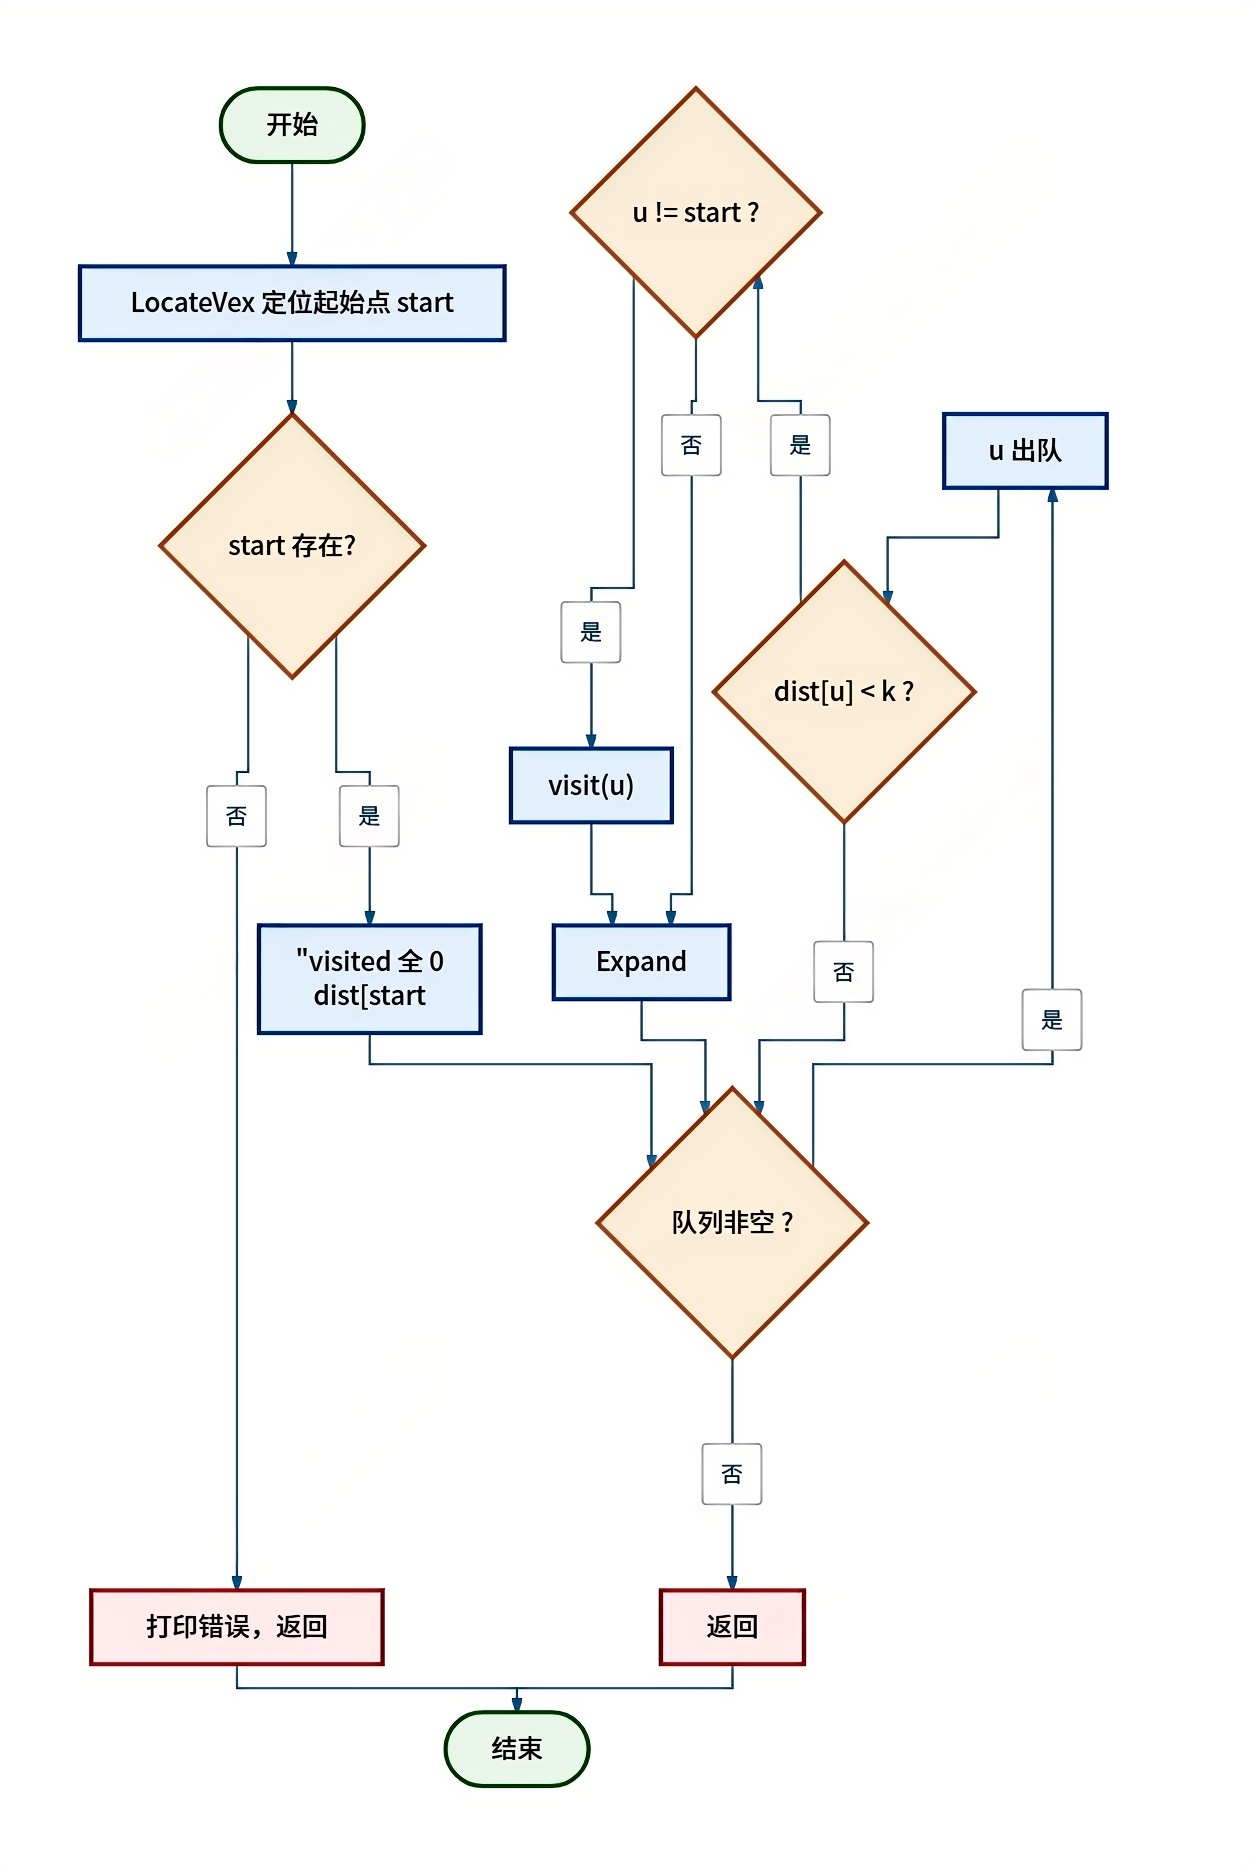
\includegraphics[width=0.85\linewidth]{距离小于K的顶点集合.png}
	\caption{距离小于K的顶点集合}
\end{figure}
\newpage
\begin{lstlisting}[label={lst:lessk}, caption={VerticesSetLessThanK}]
void VerticesSetLessThanK(ALGraph G, KeyType v, int k, void (*visit)(VertexType)) {
    int start = LocateVex(G, v);
    if (start == -1) { /* error */ return; }
    int visited[MAX_VERTEX_NUM] = {0}, dist[MAX_VERTEX_NUM];
    int queue[MAX_VERTEX_NUM], front = 0, rear = 0;
    visited[start] = 1; dist[start] = 0; queue[rear++] = start;
    while (front < rear) {
        int u = queue[front++];
        if (dist[u] < k) {
            if (u != start) visit(G.vertices[u].data);
            ArcNode *p = G.vertices[u].firstarc;
            while (p) {
                if (!visited[p->adjvex]) {
                    visited[p->adjvex] = 1;
                    dist[p->adjvex] = dist[u] + 1;
                    queue[rear++] = p->adjvex;
                }
                p = p->nextarc;
            }
        }
        // dist[u] >= k 时不再扩展邻接点（剪枝）
    }
}
\end{lstlisting}

\subsubsection{ShortestPathLength(G, v, w)——最短路径长度}
% Mermaid 参考: 图40 (ShortestPathLength) — 见 Mermaid流程图.txt

\begin{quote}\small
\textbf{初始条件：}图G存在，v和w是两个顶点关键字。\\
\textbf{操作结果：}返回顶点v与w的最短路径长度（边数），不可达时返回-1。
\end{quote}

实现分析：BFS层次遍历天然保证首次遇到终点时的dist即为最短路径长度。时间$O(n+e)$，空间$O(n)$。




\begin{lstlisting}[label={lst:shortest}, caption={ShortestPathLength}]
int ShortestPathLength(ALGraph G, KeyType v, KeyType w) {
    int start = LocateVex(G, v), end = LocateVex(G, w);
    if (start == -1 || end == -1) return -1;
    if (start == end) return 0;
    int visited[MAX_VERTEX_NUM] = {0}, dist[MAX_VERTEX_NUM];
    int queue[MAX_VERTEX_NUM], front = 0, rear = 0;
    visited[start] = 1; dist[start] = 0; queue[rear++] = start;
    while (front < rear) {
        int u = queue[front++];
        ArcNode *p = G.vertices[u].firstarc;
        while (p) {
            if (!visited[p->adjvex]) {
                visited[p->adjvex] = 1;
                dist[p->adjvex] = dist[u] + 1;
                if (p->adjvex == end) return dist[p->adjvex];
                queue[rear++] = p->adjvex;
            }
            p = p->nextarc;
        }
    }
    return -1;
}
\end{lstlisting}

\begin{figure}[htb]
	\centering
	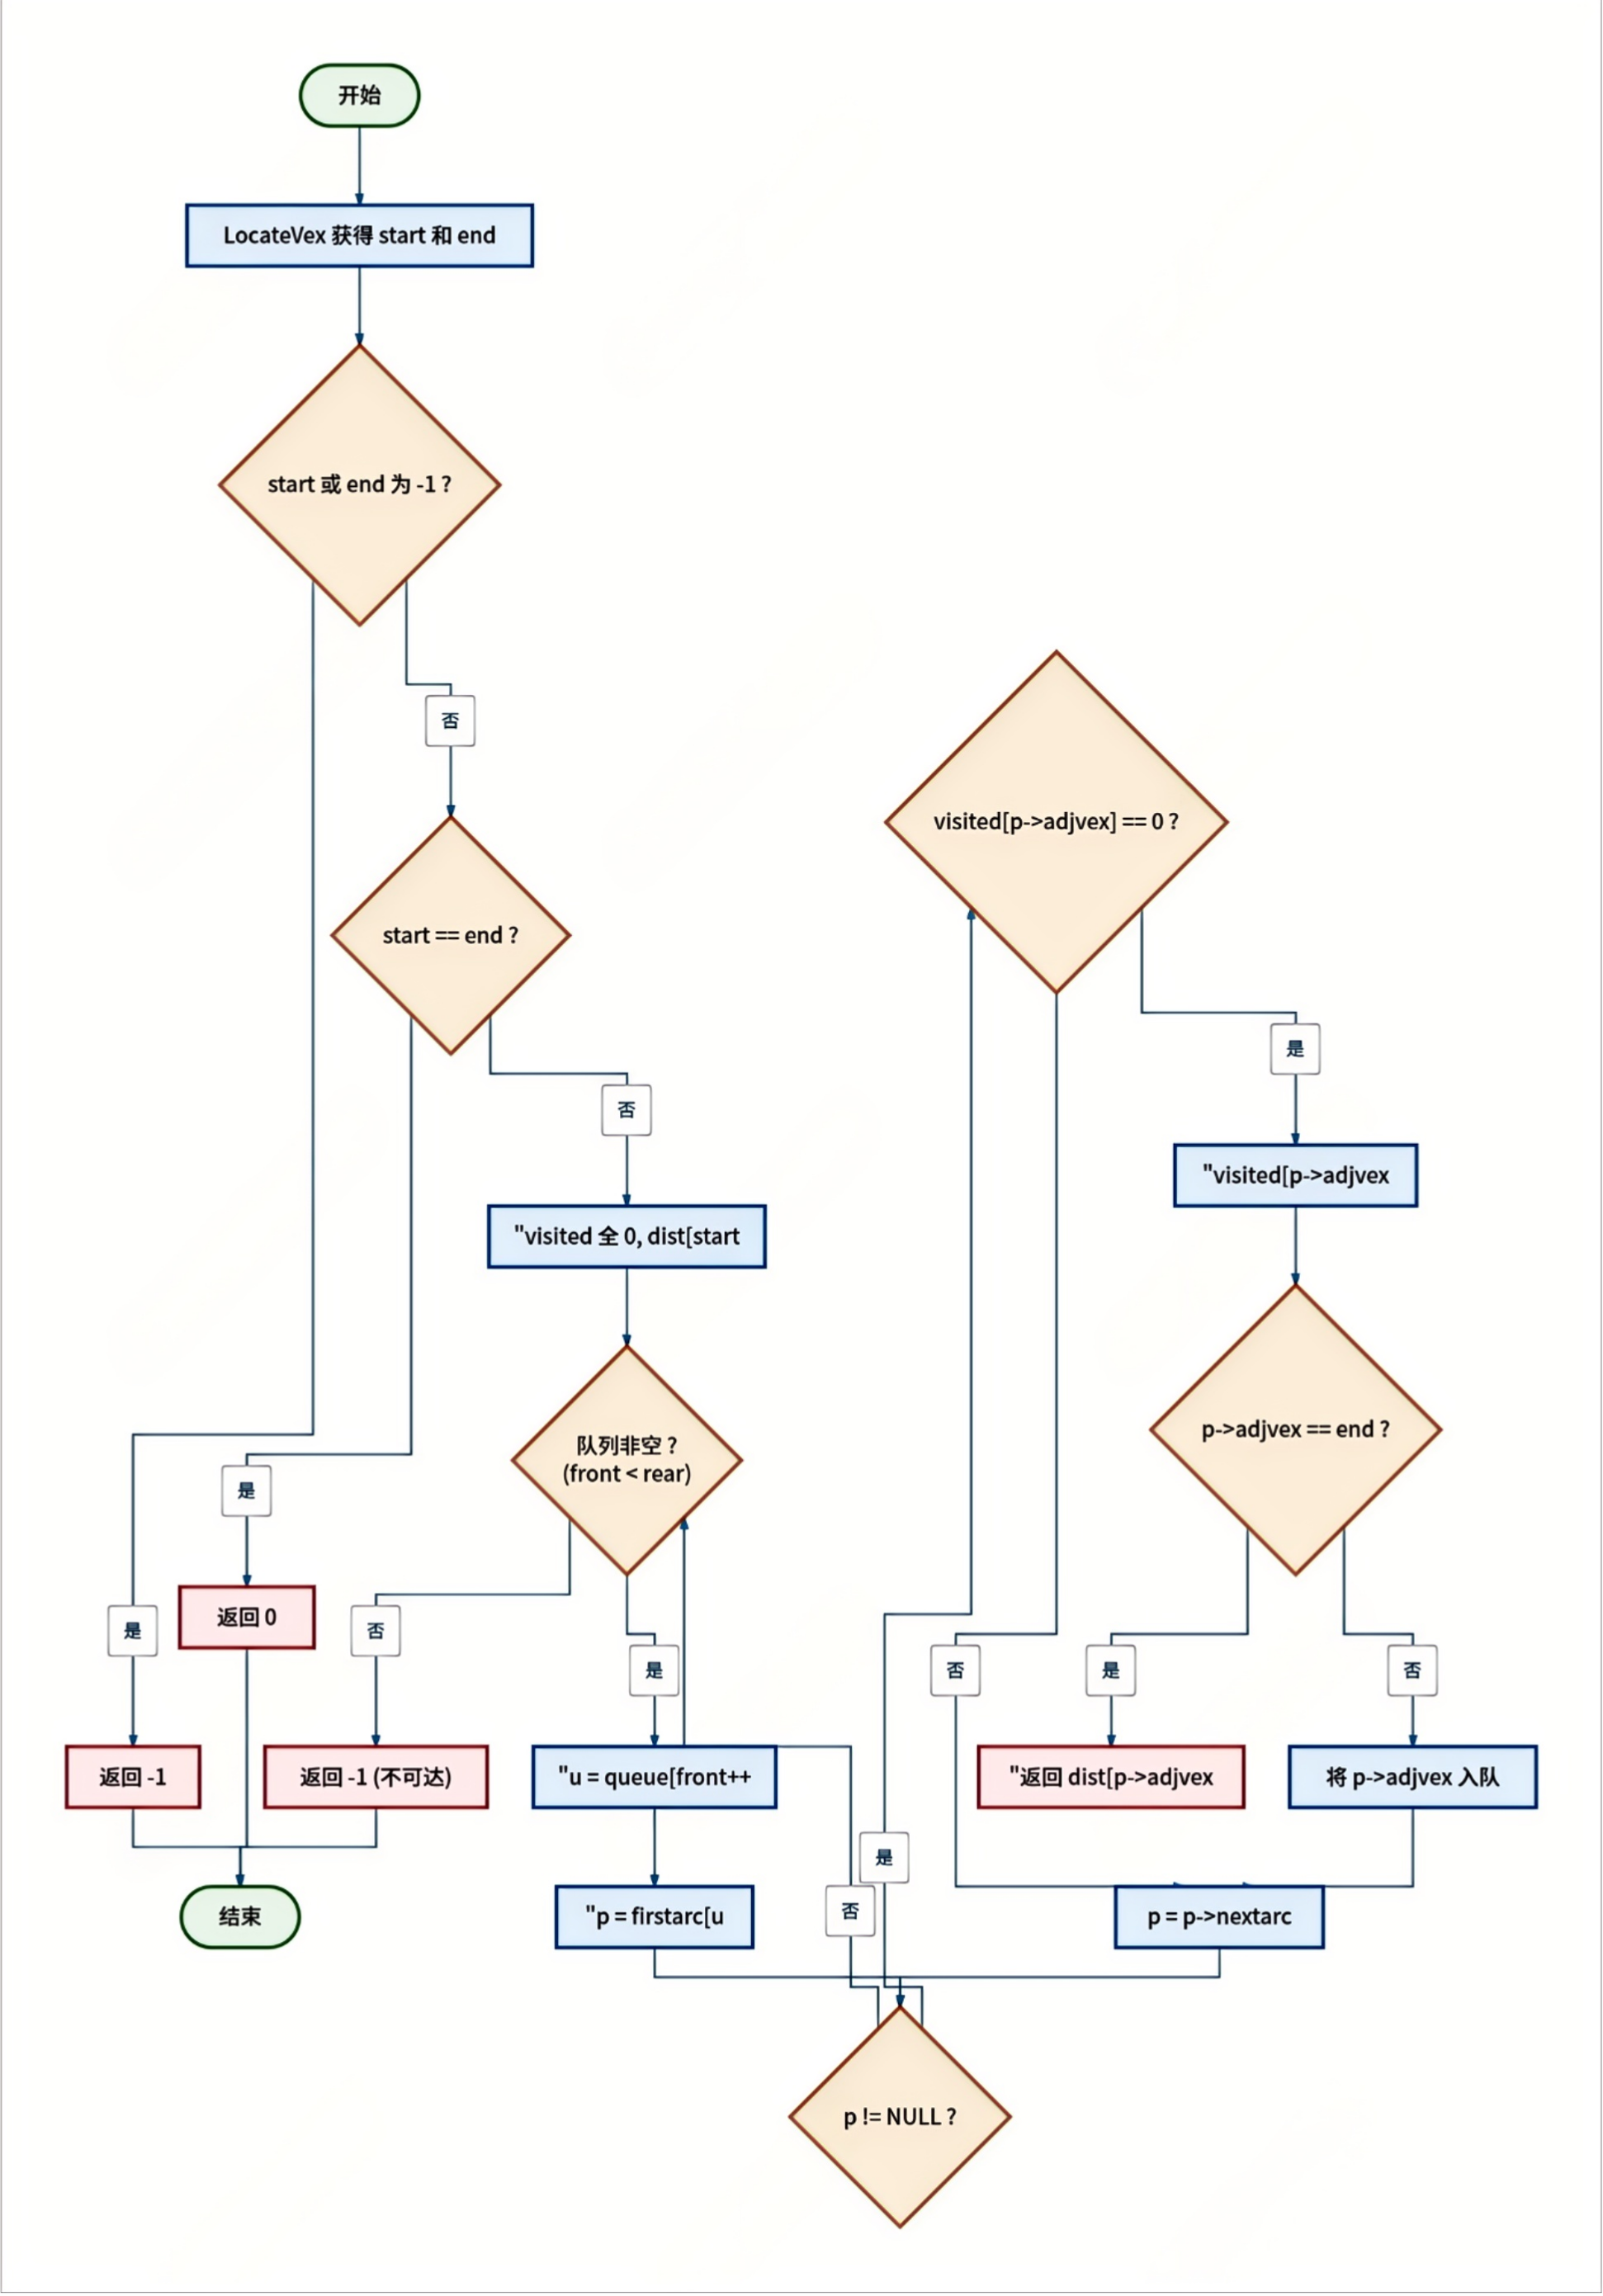
\includegraphics[width=0.6\linewidth]{最小路径长度.png}
	\caption{最短路径算法}
\end{figure}

\newpage
\subsubsection{ConnectedComponentsNums(G)——连通分量计数}
% Mermaid 参考: 图41 (ConnectedComponentsNums) — 见 Mermaid流程图.txt

\begin{quote}\small
\textbf{初始条件：}图G存在。\quad\textbf{操作结果：}返回图G的所有连通分量个数。
\end{quote}

实现分析：利用BFS的"连通区域标记"能力——外层循环扫描所有顶点，每遇未访问顶点就启动BFS标记整个连通区域并计数+1。时间$O(n+e)$。
\begin{figure}[htb]
	\centering
	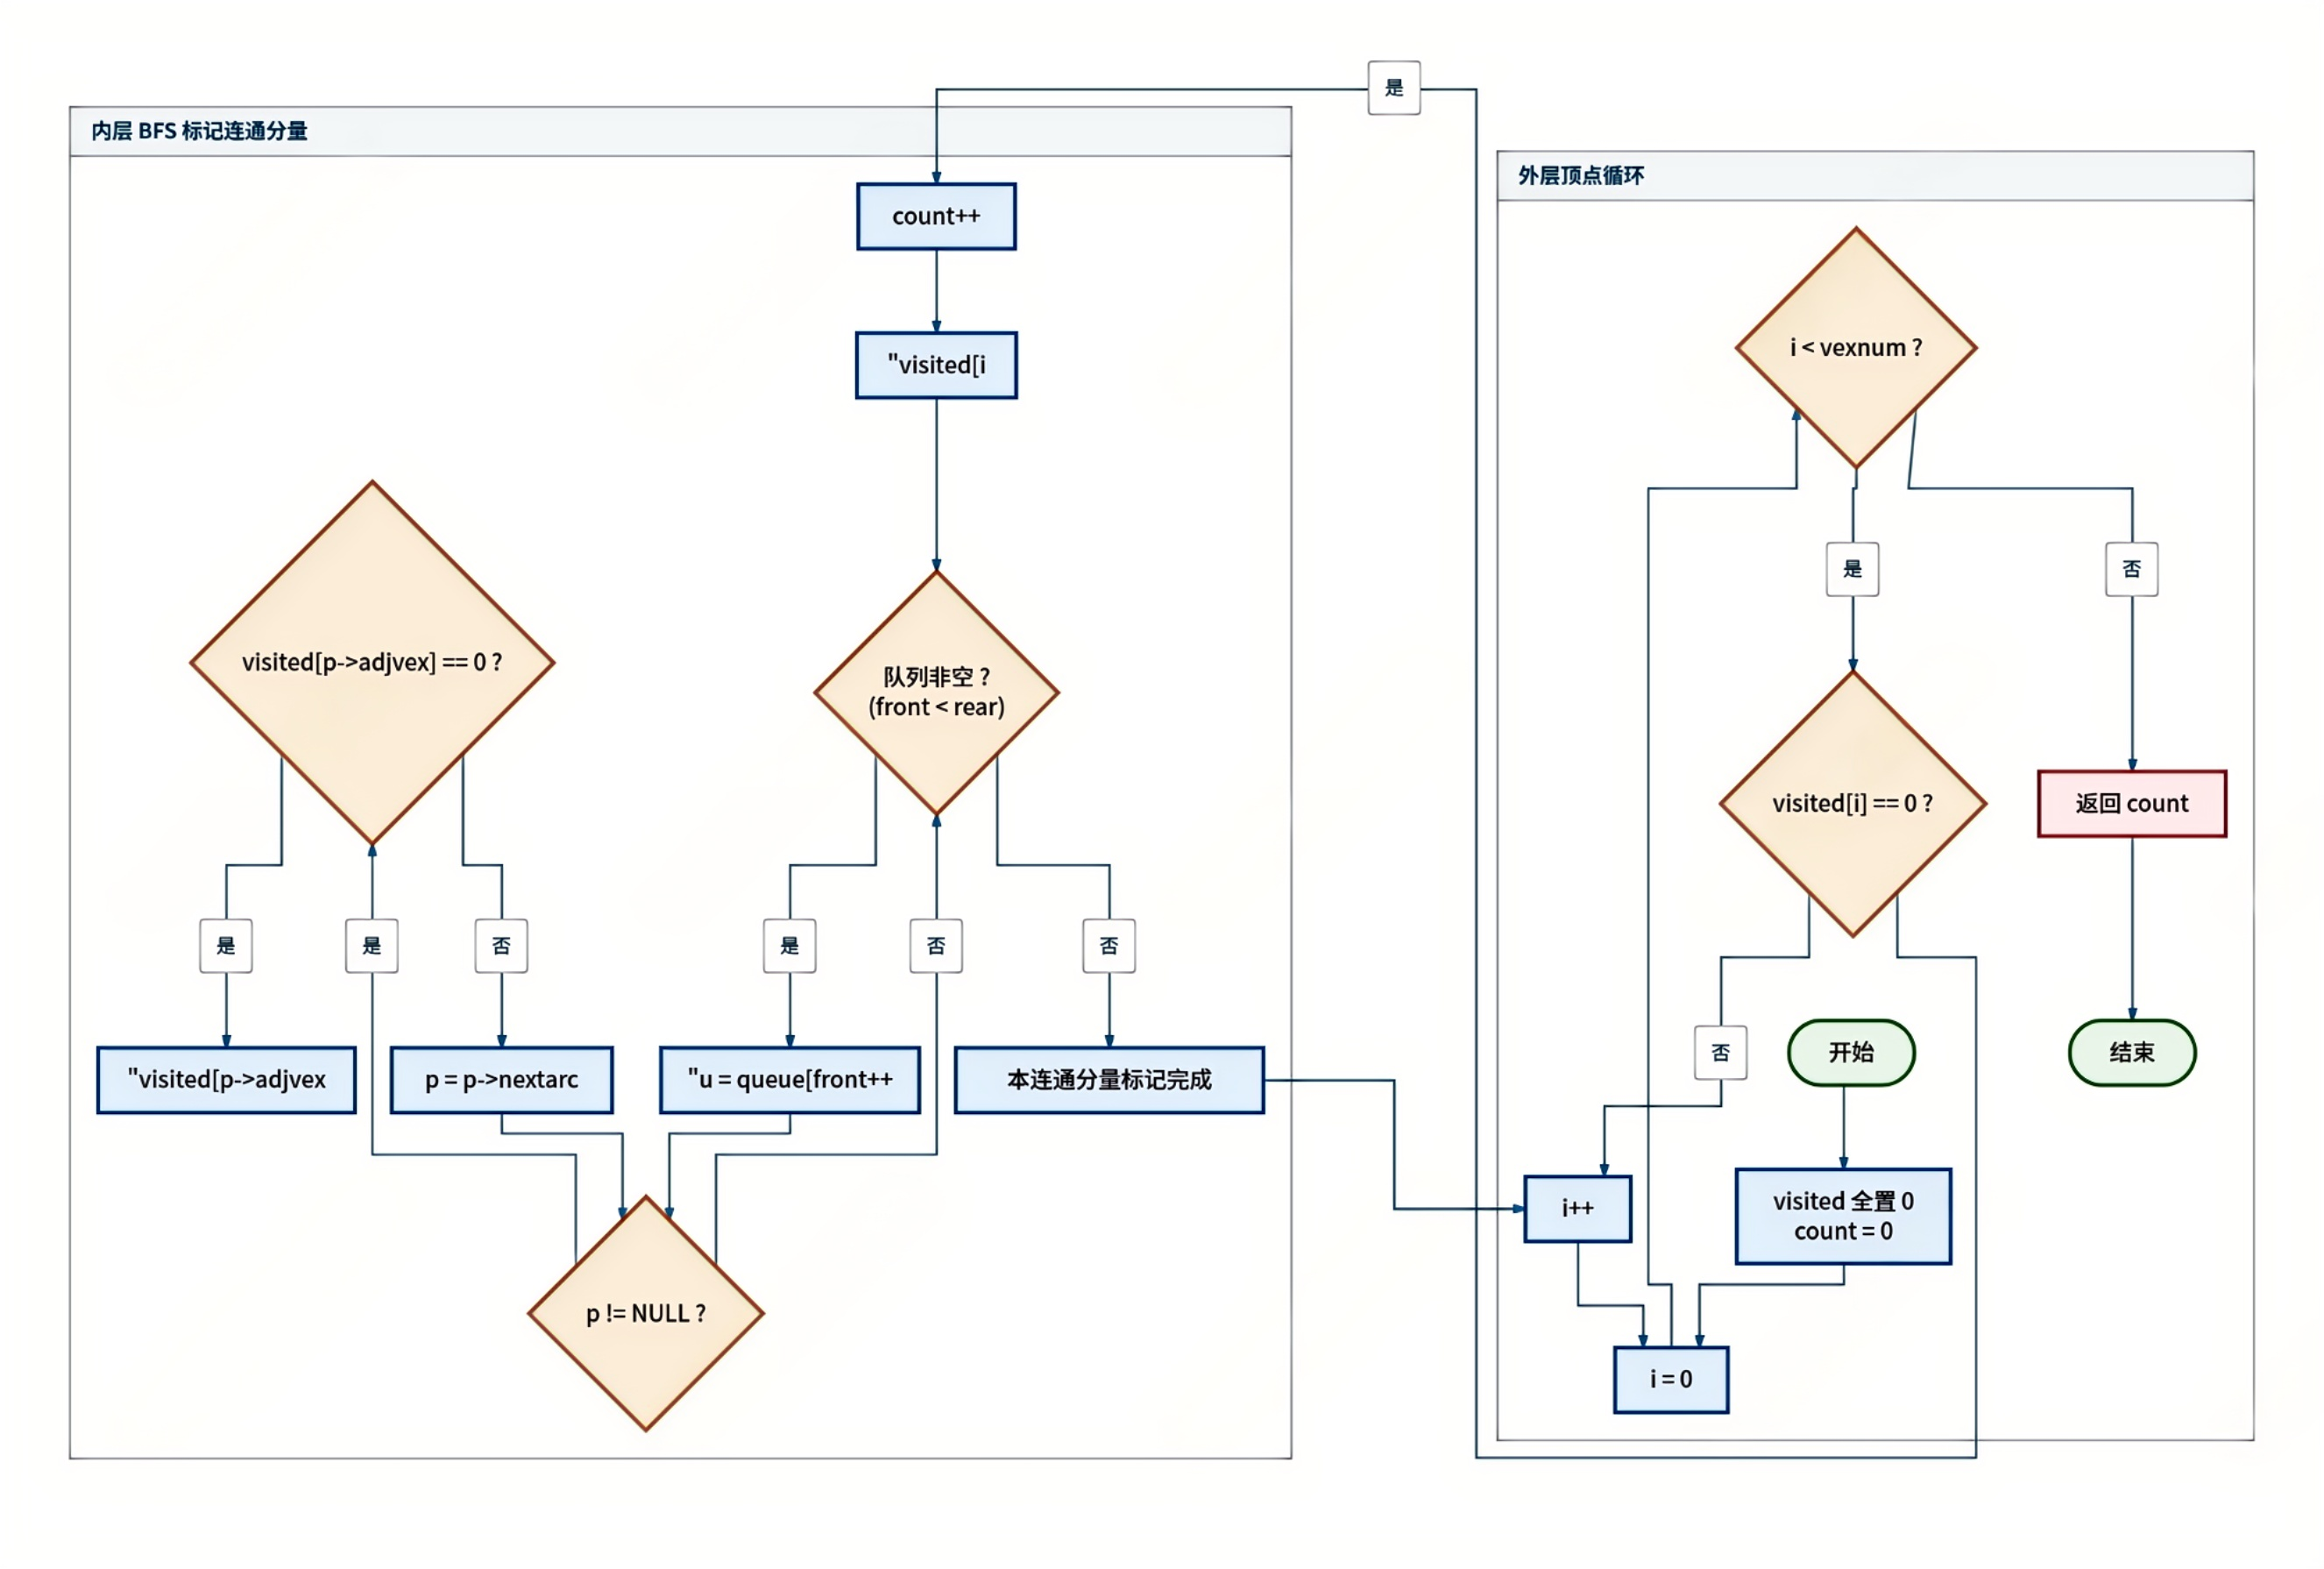
\includegraphics[width=\linewidth]{连通分量.png}
	\caption{连通分量}
\end{figure}

\begin{lstlisting}[label={lst:connect}, caption={ConnectedComponentsNums}]
int ConnectedComponentsNums(ALGraph G) {
    int visited[MAX_VERTEX_NUM] = {0}, count = 0;
    for (int i = 0; i < G.vexnum; i++) {
        if (!visited[i]) {
            count++;
            int queue[MAX_VERTEX_NUM], front = 0, rear = 0;
            visited[i] = 1; queue[rear++] = i;
            while (front < rear) {
                int u = queue[front++];
                ArcNode *p = G.vertices[u].firstarc;
                while (p) {
                    if (!visited[p->adjvex]) {
                        visited[p->adjvex] = 1;
                        queue[rear++] = p->adjvex;
                    }
                    p = p->nextarc;
                }
            }
        }
    }
    return count;
}
\end{lstlisting}




\subsubsection{文件形式保存与加载}

\begin{quote}\small
\textbf{操作结果：}设计文件数据记录格式高效保存图的数据逻辑结构(D,\{R\})完整信息；支持保存后直接加载生成图。
\end{quote}
% Mermaid 参考: 图42 (SaveGraph), 图43 (LoadGraph) — 见 Mermaid流程图.txt

\textbf{文件格式设计：}采用"顶点段+边段"的两段式文本格式：
\begin{itemize}
    \item 顶点段：\texttt{key others key others ... -1 nil}（-1为顶点终止标记）
    \item 边段：\texttt{vkey wkey vkey wkey ... -1 -1}（-1 -1为边终止标记）
\end{itemize}
\textbf{关键优化：}每条无向边只写一次（条件\texttt{p->adjvex > i}），避免重复存储。\textbf{LoadGraph}逆向解析——先读顶点段重建邻接表头，再读边段创建ArcNode并插入邻接表。


\begin{figure}[htb]
	\centering
	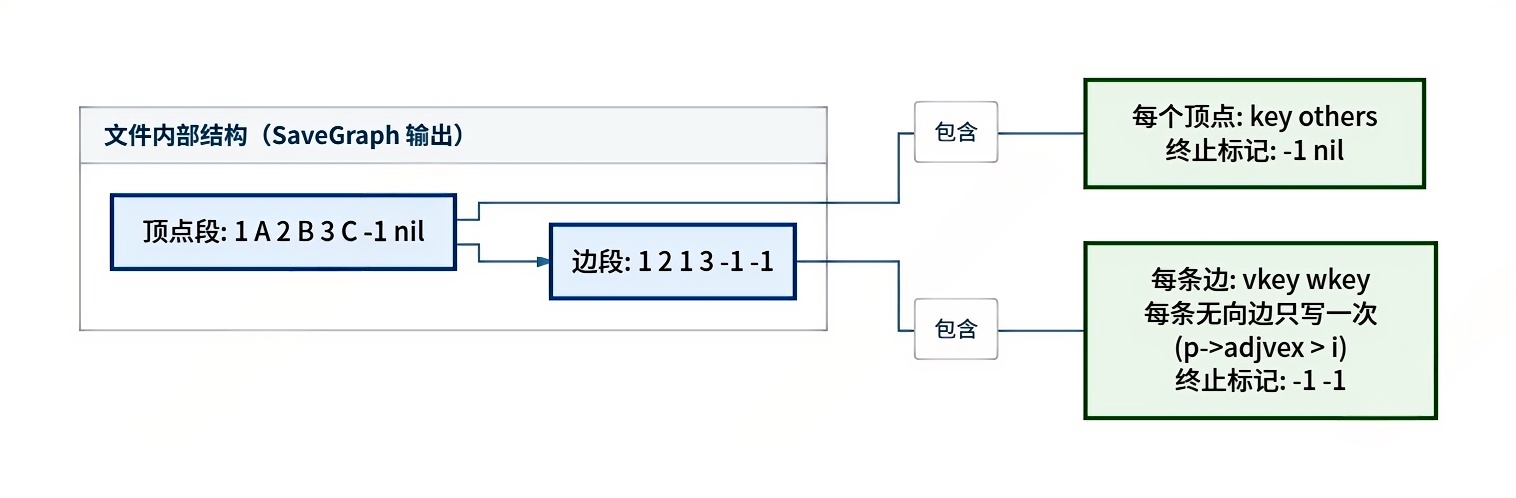
\includegraphics[width=\linewidth]{文件结构图.png}
	\caption{存储结构图}
\end{figure}
由于排版问题，文件操作的具体设计转下页图2-17和Listing 35：

\newpage

\begin{figure}[H]
	\centering
	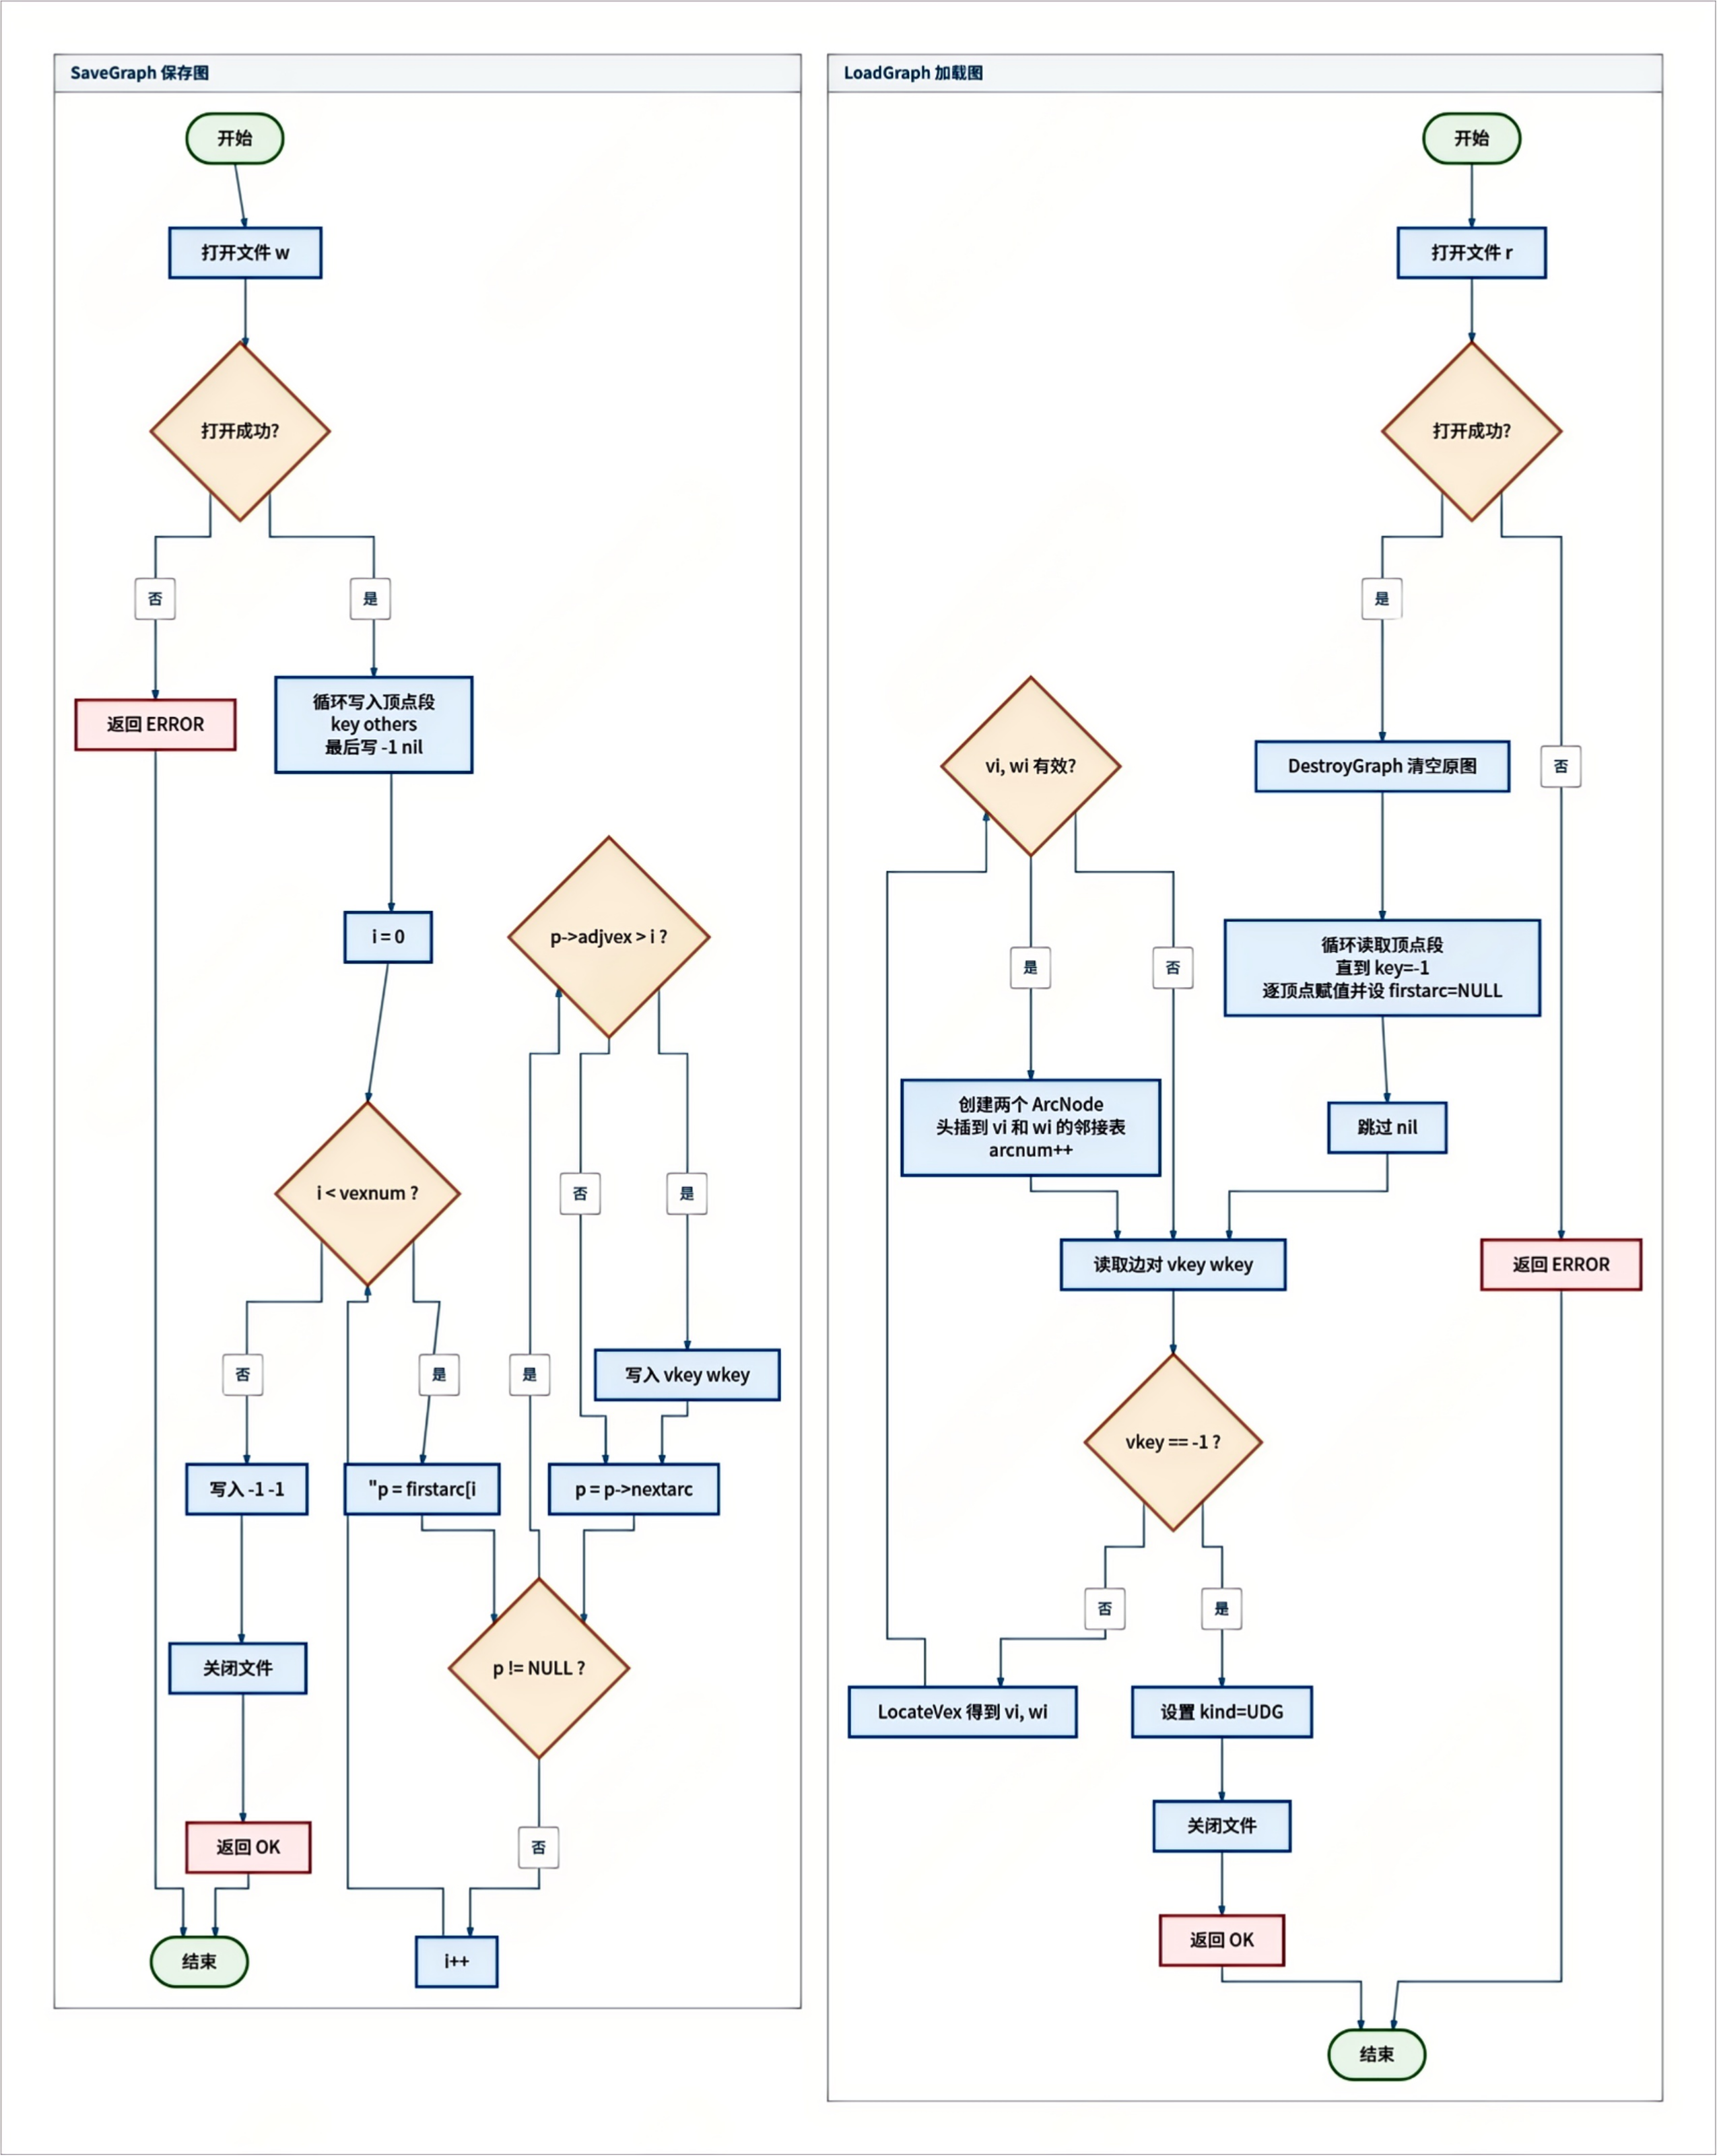
\includegraphics[width=\linewidth]{文件存储.png}
	\caption{文件操作流程图}
\end{figure}


\begin{lstlisting}[label={lst:save-graph}, caption={SaveGraph与LoadGraph}]
status SaveGraph(ALGraph G, char FileName[]) {
    FILE *fp = fopen(FileName, "w");
    if (fp == NULL) return ERROR;
    for (int i = 0; i < G.vexnum; i++)
        fprintf(fp, "%d %s ", G.vertices[i].data.key, G.vertices[i].data.others);
    fprintf(fp, "-1 nil ");
    for (int i = 0; i < G.vexnum; i++) {
        ArcNode *p = G.vertices[i].firstarc;
        while (p) {
            if (p->adjvex > i)  // 每条边只写一次
                fprintf(fp, "%d %d ", G.vertices[i].data.key, G.vertices[p->adjvex].data.key);
            p = p->nextarc;
        }
    }
    fprintf(fp, "-1 -1"); fclose(fp);
    return OK;
}
status LoadGraph(ALGraph *G, char FileName[]) {
    FILE *fp = fopen(FileName, "r");
    if (fp == NULL) return ERROR;
    DestroyGraph(G);
    int key; char others[20];
    while (fscanf(fp, "%d", &key)==1 && key!=-1) {
        fscanf(fp, "%s", others);
        G->vertices[G->vexnum].data.key = key;
        strcpy(G->vertices[G->vexnum].data.others, others);
        G->vertices[G->vexnum].firstarc = NULL;
        G->vexnum++;
    }
    char nilbuf[10]; fscanf(fp, "%s", nilbuf);
    int vkey, wkey;
    while (fscanf(fp, "%d %d", &vkey,&wkey)==2 && vkey!=-1) {
        int vi=LocateVex(*G,vkey), wi=LocateVex(*G,wkey);
        if (vi!=-1 && wi!=-1 && vi!=wi) {
            ArcNode *a1=(ArcNode*)malloc(sizeof(ArcNode));
            a1->adjvex=wi; a1->nextarc=G->vertices[vi].firstarc;
            G->vertices[vi].firstarc=a1;
            ArcNode *a2=(ArcNode*)malloc(sizeof(ArcNode));
            a2->adjvex=vi; a2->nextarc=G->vertices[wi].firstarc;
            G->vertices[wi].firstarc=a2;
            G->arcnum++;
        }
    }
    fclose(fp); G->kind=UDG;
    return OK;
}
\end{lstlisting}
\newpage


\subsection{多图管理功能分析}

\subsubsection{数据结构设计——与多表管理的对称性}

多图管理的GRAPHS结构体与多表管理的LISTS结构体在设计上完全对称：结构体数组 + length计数 + 名称索引 + currentIdx光标。GRAPHS结构体定义如下：
\begin{itemize}
    \item \texttt{NamedGraph elem[MAX\_GRAPH\_NUM]}——固定容量（10个）的命名图数组，每个NamedGraph含\texttt{char name[20]}（唯一标识符）和\texttt{ALGraph G}（完整邻接表图结构体）
    \item \texttt{int length}——当前实际存储的图数量
\end{itemize}

尽管设计模式对称，两种结构体在内含元素的内存形态上存在本质差异：
\begin{itemize}
    \item LISTS的NamedList存储\texttt{LinkList L}——指针（8字节），指向堆上独立分配的单链表
    \item GRAPHS的NamedGraph存储\texttt{ALGraph G}——完整结构体，包含20个VNode（约640+字节）
\end{itemize}

这一差异导致初始化策略的不同：ALGraph可通过直接赋零值表达"空图"（vexnum=0），而LinkList的"空"需要malloc头节点（资源获取）。

\begin{figure}[htb]
	\centering
	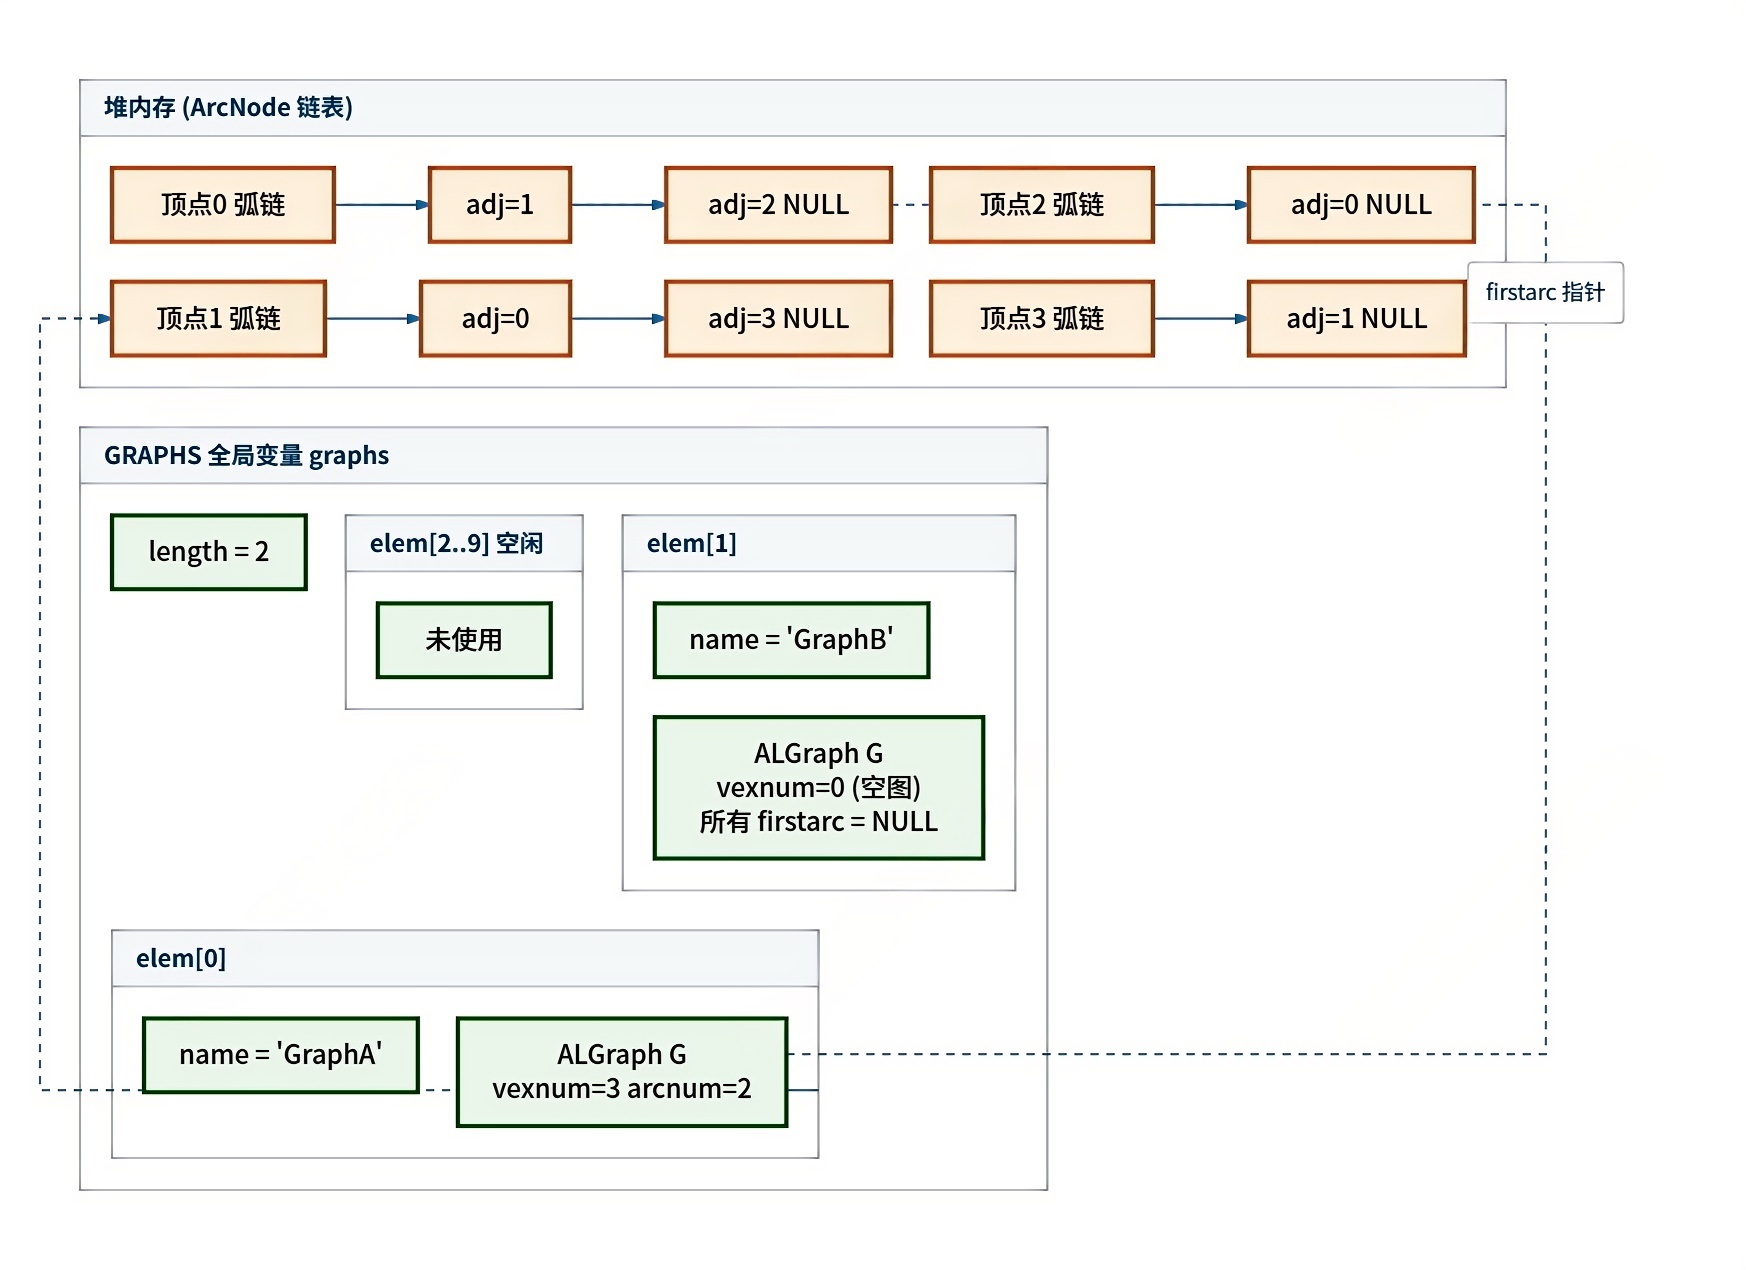
\includegraphics[width=\linewidth]{多图管理结构图.png}
	\caption{多图管理结构图}
\end{figure}

多表管理与多图管理的关键差异汇总如下：

\begin{table}[!htb]\centering
\caption{多表管理与多图管理的关键差异}
\label{tbl:multi-compare}\renewcommand\arraystretch{1.3}
\begin{tabular}{|c|c|c|}
\hline
\textbf{对比维度} & \textbf{多表管理 (LISTS)} & \textbf{多图管理 (GRAPHS)} \\
\hline
元素类型 & NamedList (含LinkList指针) & NamedGraph (含ALGraph结构体) \\
单个元素内存 & ~44字节 & ~680字节 \\
初始化策略 & L设为NULL，延迟初始化 & 立即将G置为"空图" \\
原因 & InitList需malloc头节点 & 结构体字段可直接赋零值 \\
删除时资源释放 & DestroyList→释放LNode & DestroyGraph→释放ArcNode \\
元素的"空"状态 & L==NULL & vexnum==0 \\
\hline
\end{tabular}
\end{table}

\subsubsection{AddGraph——添加图}
% Mermaid 参考: 图44 (AddGraph) — 见 Mermaid流程图.txt

\texttt{AddGraph(GRAPHS *Graphs, char GraphName[])}在GRAPHS数组尾部追加一个新的命名图条目。初始条件是容量未满且名称不重复，操作结果是在elem[length]位置创建空图并递增length。

与多表管理的AddList不同，AddGraph在创建时立即初始化图的所有字段为合法状态：
\begin{enumerate}
    \item 检查容量（\texttt{length >= MAX\_GRAPH\_NUM}）和名称唯一性（遍历已有图名用\texttt{strcmp}比较）
    \item 复制名称字符串
    \item 将G的\texttt{vexnum}和\texttt{arcnum}设为0、\texttt{kind}设为UDG
    \item 将所有20个顶点的\texttt{firstarc}指针置为NULL（循环边界为\texttt{MAX\_VERTEX\_NUM}而非当前\texttt{vexnum}，因为vertices数组的所有槽位已存在，需确保firstarc不含垃圾值）
\end{enumerate}

立即初始化的原因在于ALGraph是值类型结构体——其"空"状态可由自身字段完整表达，无需像LinkList那样等待外部资源分配。

\begin{lstlisting}[caption={AddGraph函数}]
status AddGraph(GRAPHS *Graphs, char GraphName[]) {
    if (Graphs->length >= MAX_GRAPH_NUM) return ERROR;
    int i;
    for (i = 0; i < Graphs->length; i++)
        if (strcmp(Graphs->elem[i].name, GraphName) == 0) return ERROR;
    strcpy(Graphs->elem[Graphs->length].name, GraphName);
    Graphs->elem[Graphs->length].G.vexnum = 0;
    Graphs->elem[Graphs->length].G.arcnum = 0;
    Graphs->elem[Graphs->length].G.kind = UDG;
    for (i = 0; i < MAX_VERTEX_NUM; i++)
        Graphs->elem[Graphs->length].G.vertices[i].firstarc = NULL;
    Graphs->length++;
    return OK;
}
\end{lstlisting}

\subsubsection{RemoveGraph——删除图}
% Mermaid 参考: 图45 (RemoveGraph) — 见 Mermaid流程图.txt

\texttt{RemoveGraph(GRAPHS *Graphs, char GraphName[])}按名称查找并删除指定图。函数分三步执行：线性搜索→DestroyGraph释放图资源→数组前移。资源释放与数组移动的顺序与RemoveList遵循同一原则：先释放再移动。DestroyGraph涉及嵌套循环（外层遍历顶点数组、内层遍历弧链），释放的节点数量为$n+e$，在最坏情况（20顶点的完全图，190条边）下需释放数百个ArcNode。

\begin{lstlisting}[caption={RemoveGraph函数}]
status RemoveGraph(GRAPHS *Graphs, char GraphName[]) {
    int pos = -1, i;
    for (i = 0; i < Graphs->length; i++)
        if (strcmp(Graphs->elem[i].name, GraphName) == 0)
            { pos = i; break; }
    if (pos == -1) return ERROR;
    DestroyGraph(&Graphs->elem[pos].G);
    for (i = pos; i < Graphs->length - 1; i++)
        Graphs->elem[i] = Graphs->elem[i + 1];
    Graphs->length--;
    return OK;
}
\end{lstlisting}

\subsubsection{LocateGraph与ListAllGraphs}
% Mermaid 参考: 图46 (LocateGraph) — 见 Mermaid流程图.txt

\texttt{LocateGraph(GRAPHS Graphs, char GraphName[])}顺序扫描返回匹配名称的元素序号（从1开始），未找到返回0。\texttt{ListAllGraphs(GRAPHS Graphs)}遍历所有命名图，以彩色格式输出序号、名称、顶点数和边数，其中名称用绿色(10)突出显示，顶点数和边数为辅助信息的青色(11)。

\subsubsection{multiGraphMode——交互控制逻辑}
% Mermaid 参考: 图47 (multiGraphMode 状态转换) — 见 Mermaid流程图.txt

\texttt{multiGraphMode()}的交互逻辑与多表管理的\texttt{multiTableMode()}完全对称，维护\texttt{currentIdx}变量（初始为-1表示未选中），通过顶层菜单支持五种操作：

\begin{enumerate}
    \item \textbf{新建图（case 1）}：读取图名，调用\texttt{AddGraph}追加。新建后的图为空（vexnum=0），用户需随后选择图并进入图操作菜单通过建图功能输入顶点和边。
    \item \textbf{选择图（case 2）}：读取图名，调用\texttt{LocateGraph}查找。若找到则设置\texttt{currentIdx = idx - 1}，后续通过\texttt{\&graphs.elem[currentIdx].G}定位当前图。
    \item \textbf{删除图（case 3）}：读取图名，调用\texttt{RemoveGraph}。若被删图为当前选中图，将\texttt{currentIdx}重置为-1。
    \item \textbf{操作当前图（case 4）}：检查\texttt{currentIdx != -1}后调用\texttt{operateGraphMenu(\&graphs.elem[currentIdx].G)}进入图操作菜单。
    \item \textbf{返回上级（case 5）}：退出multiGraphMode。
\end{enumerate}

多图管理存在一个语义差异：新建图后图已处于"空图"合法状态，用户进入图操作菜单后选择建图（case 1）即可输入顶点序列和边序列构造图，无需先执行类似InitList的初始化步骤。这与多表管理中"新建表后需手动初始化"形成对比，根源在于两种数据结构的"空"语义不同。

\begin{figure}[htb]
	\centering
	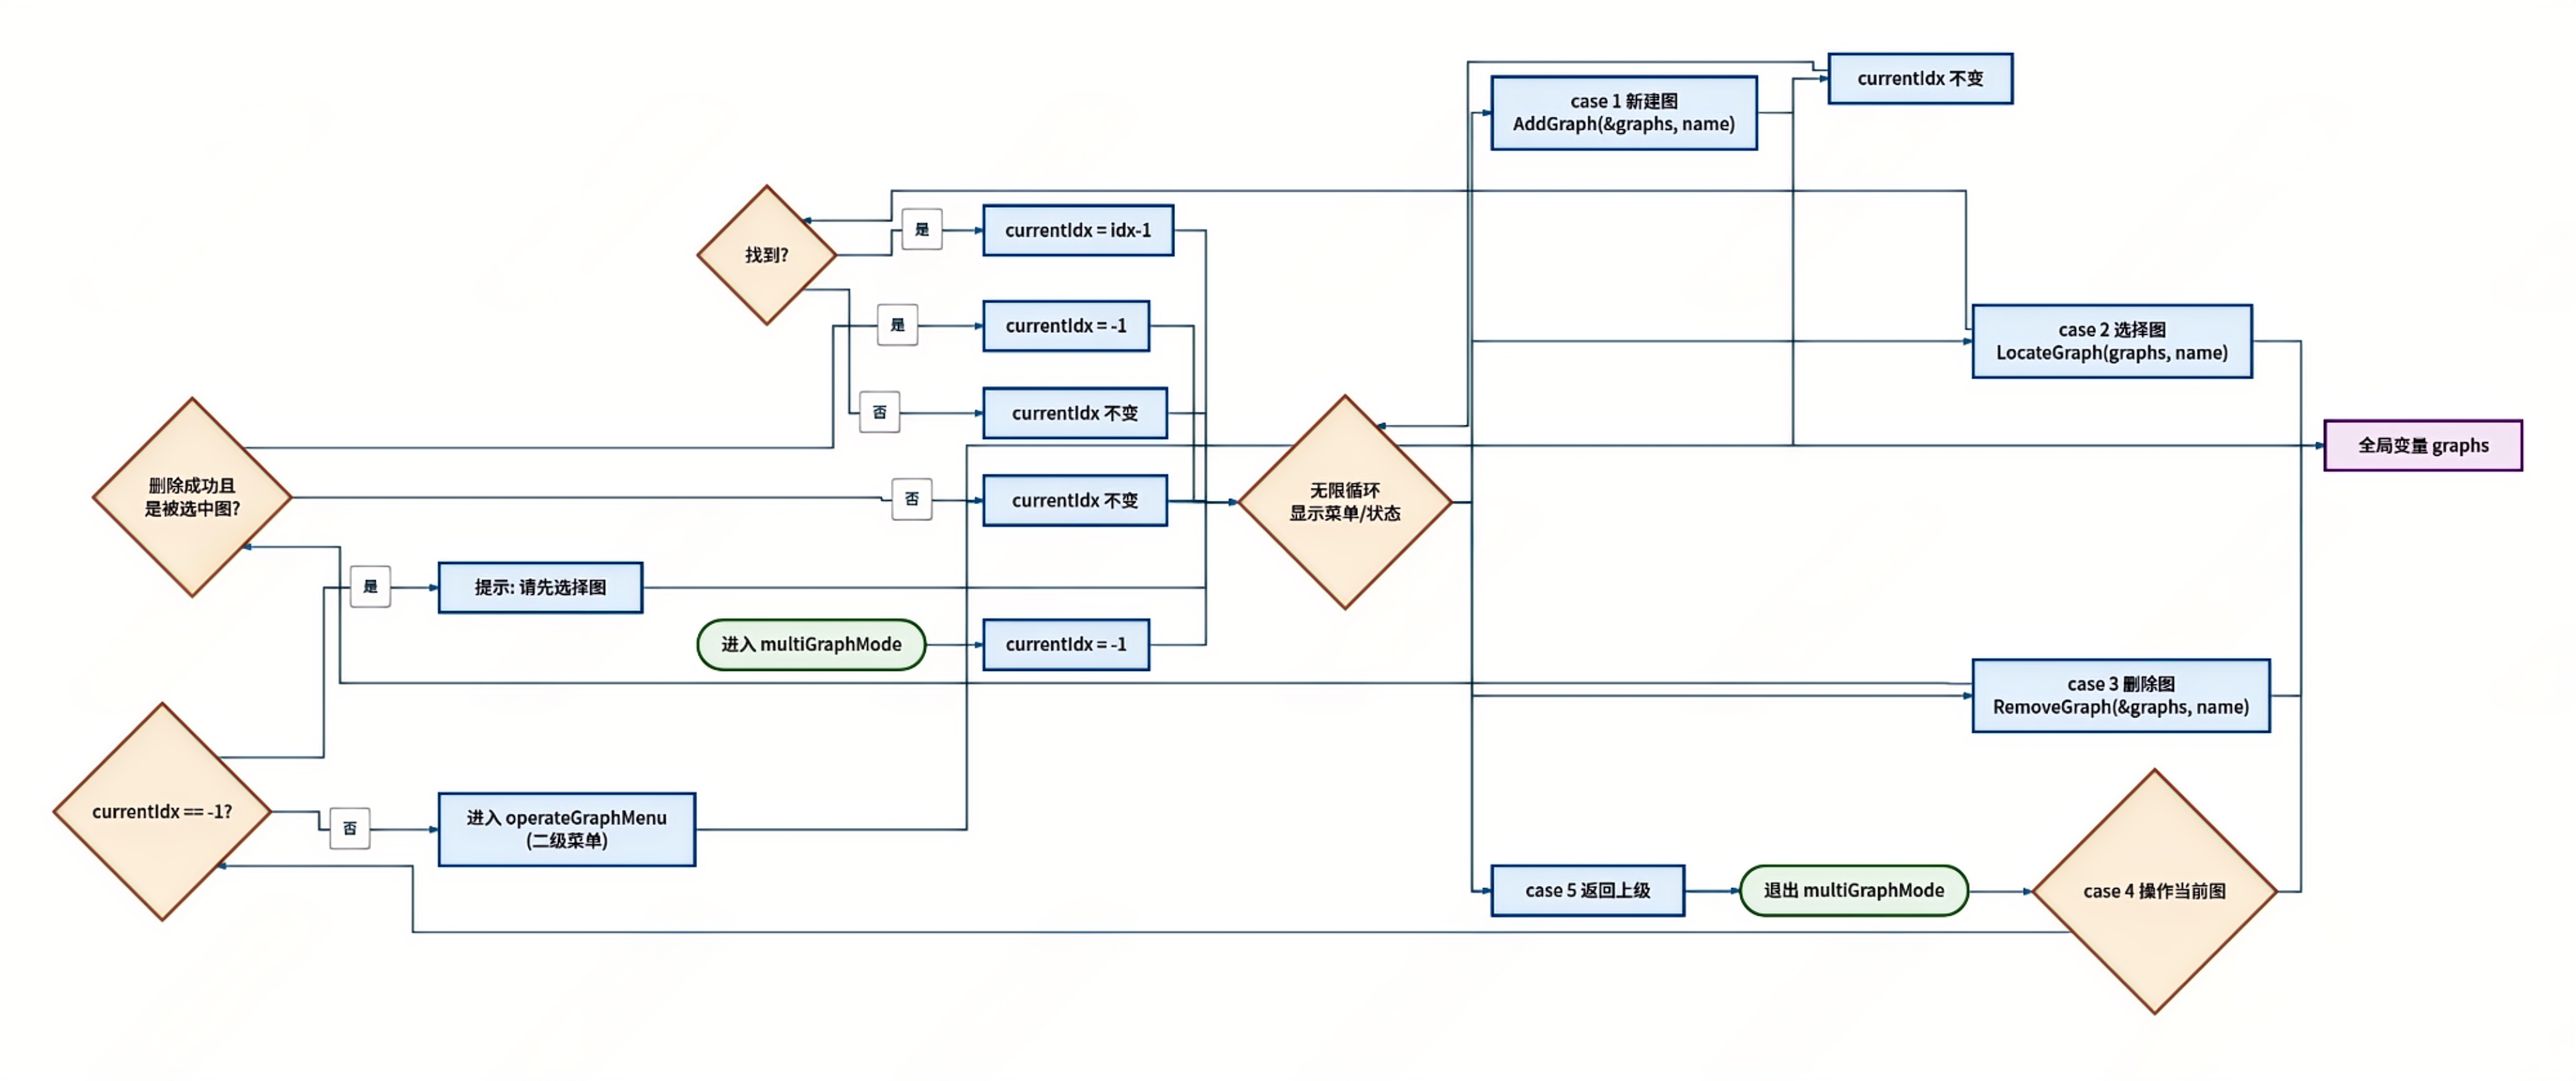
\includegraphics[width=\linewidth]{多图管理控制逻辑.png}
	\caption{多图管理交互控制}
\end{figure}


\subsubsection{设计模式总结}
% Mermaid 参考: 图49 (实验二main主函数) — 见 Mermaid流程图.txt
% Mermaid 参考: 图48 (命名对象容器设计模式) — 见 Mermaid流程图.txt

两个实验的多对象管理采用统一的容器模式：将多个命名对象组织在结构体数组中，以length记录有效元素数量，以currentIdx定位当前操作对象（充当光标），提供Add/Remove/Locate作为基本CRUD操作。这种模式可视为顺序表在元数据层面的应用——外层用顺序表（数组）管理对象索引，内层用链式结构（单链表/邻接表）管理具体数据，每种存储结构在各自最合适的层面发挥作用。
\newpage

\subsection{算法复杂度汇总}

\begin{table}[H]\centering
\caption{图各操作算法复杂度（n顶点数，e边数）}
\label{tbl:complexity2}\renewcommand\arraystretch{1.2}
\begin{tabular}{|c|c|c|c|}\hline
\textbf{操作} & \textbf{函数} & \textbf{时间} & \textbf{空间} \\\hline
建图 & CreateGraph & $O(n^2+e)$ & $O(n+e)$ \\\hline
销毁/遍历/定位 & DestroyG/DFST/BFST/LocateV & $O(n+e)$ & $O(n)$ \\\hline
赋值/首邻接/插顶点 & PutVex/FirstAdj/InsertVex & $O(n)$ & $O(1)$ \\\hline
下一邻接点 & NextAdjVex & $O(n+e)$ & $O(1)$ \\\hline
删除顶点 & DeleteVex & $O(n+e)$ & $O(1)$ \\\hline
插入/删除边 & InsertArc/DeleteArc & $O(n+e)$ & $O(1)$ \\\hline
三个BFS应用 & LessThanK/Shortest/CC & $O(n+e)$ & $O(n)$ \\\hline
文件保存/加载 & SaveGraph/LoadGraph & $O(n+e)$ & $O(1)$ \\\hline
\end{tabular}
\end{table}

\subsection{实验四小结}

\begin{enumerate}
    \item \textbf{邻接表空间效率}：$O(n+e)$在稀疏图中远优于邻接矩阵$O(n^2)$。但边存在性判断（需遍历弧链）和顶点删除（需全局下标校正）暴露了链式结构改操作的代价。
    \item \textbf{DFS与BFS的本质差异}：DFS用栈深入回溯，BFS用队列逐层扩展。在无权图中BFS天然保证最短路径，这是其三应用（ShortestPathLength、VerticesSetLessThanK、ConnectedComponentsNums）的理论基础。
    \item \textbf{DeleteVex四步全局同步}：统计→清理引用→释放自身→下标重映射。adjvex校正（\texttt{if (adjvex>i) adjvex--}）体现了"数组下标作为引用时需全局维护"的数据结构原理。
    \item \textbf{文件格式的巧妙设计}：顶点段+边段的两段式格式配合"每条边只写一次"（adjvex>i条件）实现了无冗余的高效持久化。
\end{enumerate}

\newpage

\subsection{程序测试结果截图示例}
\vspace{-1em}
以下按照实验任务书的测试要求，依次展示基于邻接表的图演示系统各项功能运行结果。测试环境为 Windows 11 + MinGW g++。


\begin{figure}[!htb]
\centering
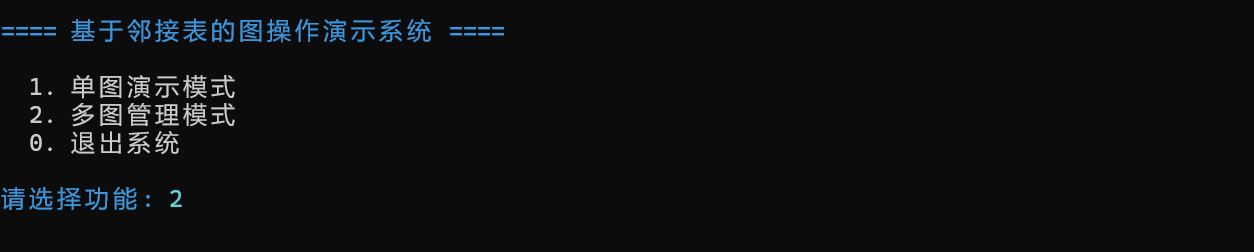
\includegraphics[width=0.75\textwidth]{images/t4_exam4_image1.png}\vspace{2pt}
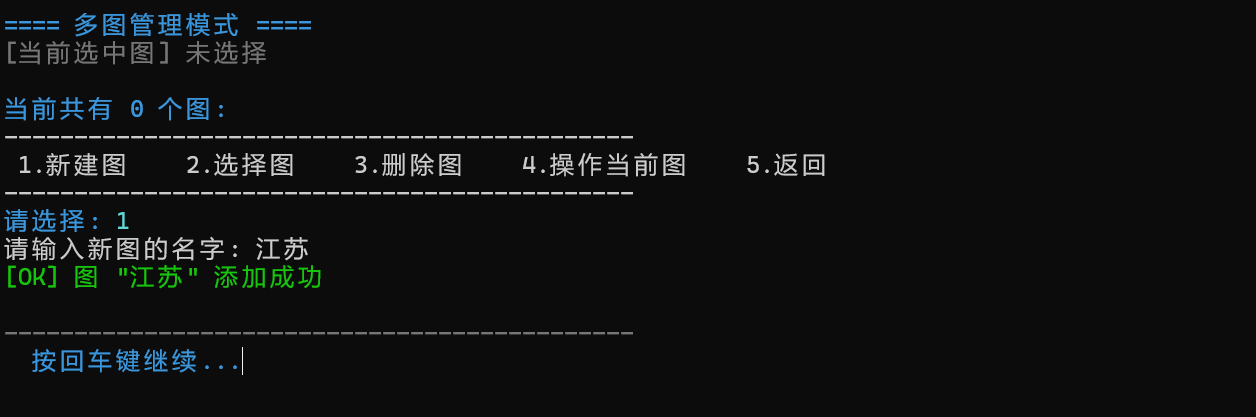
\includegraphics[width=0.75\textwidth]{images/t4_exam4_image2.png}\vspace{2pt}
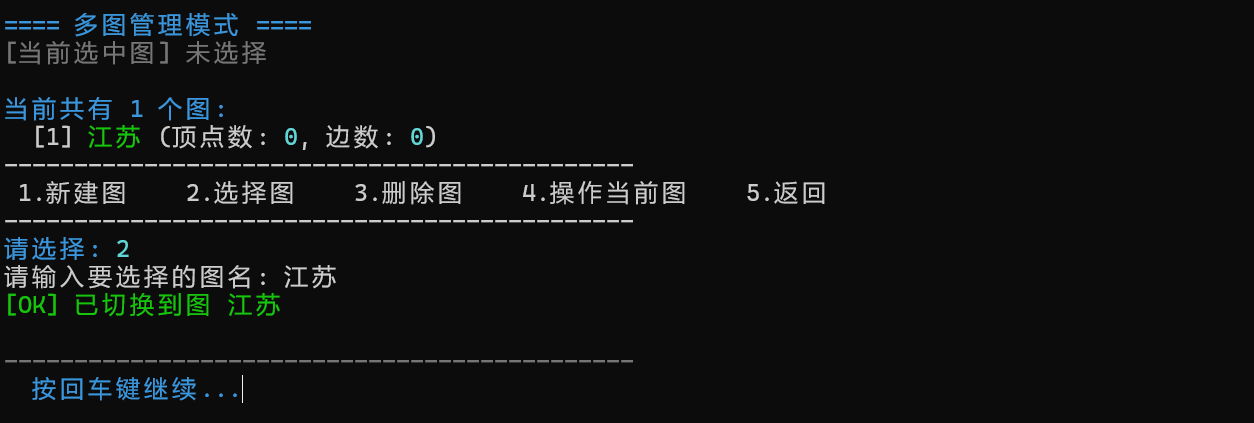
\includegraphics[width=0.75\textwidth]{images/t4_exam4_image3.png}\vspace{2pt}
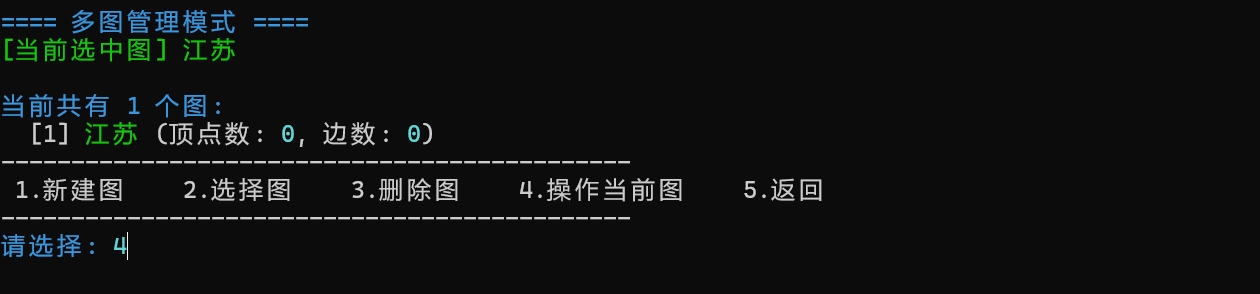
\includegraphics[width=0.75\textwidth]{images/t4_exam4_image4.png}\vspace{2pt}

\includegraphics[width=0.75\textwidth]{images/t4_exam4_image5.png}
\caption{多图管理模式下创建名为"江苏"的图，进入单图操作菜单并初始化邻接表}
\label{fig:exam4-create-js}
\end{figure}
\newpage
\begin{figure}[!htb]
\centering
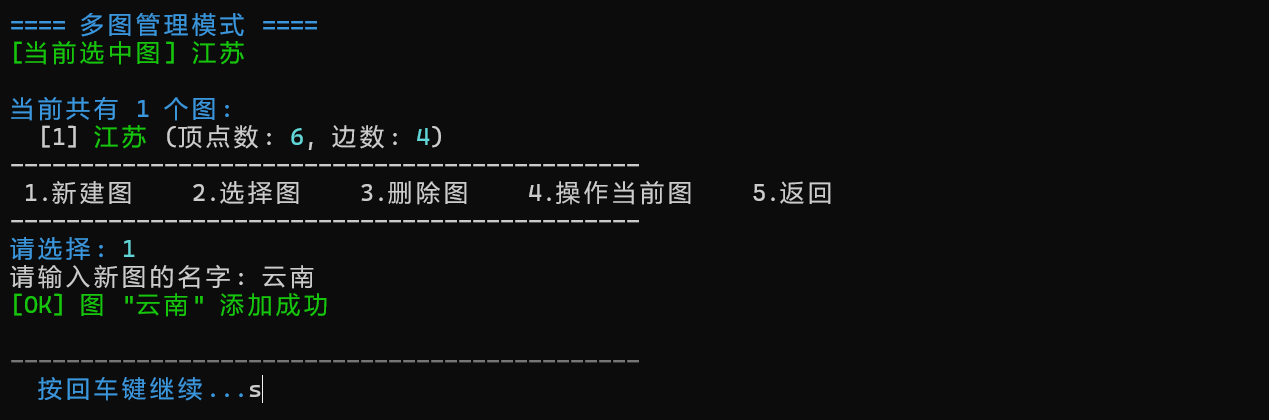
\includegraphics[width=0.75\textwidth]{images/t4_exam4_image20.png}\vspace{2pt}
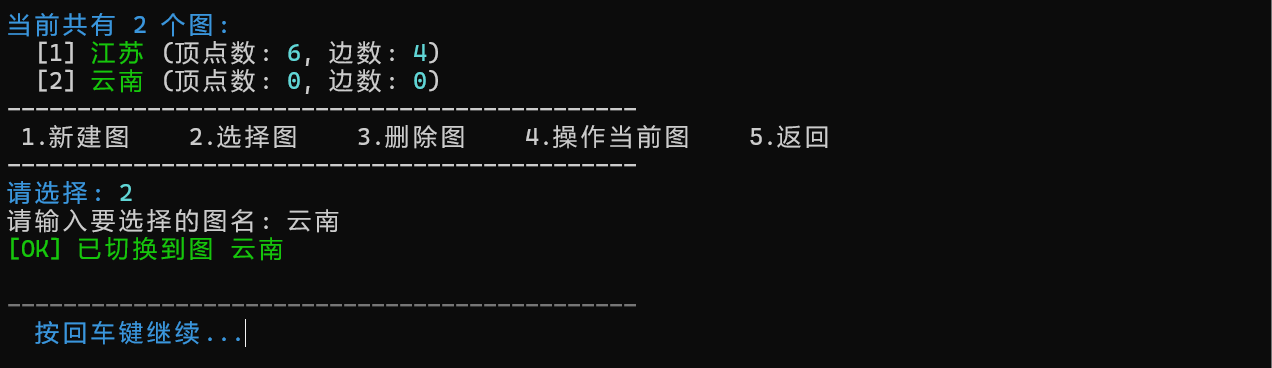
\includegraphics[width=0.75\textwidth]{images/t4_exam4_image21.png}
\caption{多图管理模式下创建名为"云南"的图，进入单图操作菜单并初始化邻接表}
\label{fig:exam4-create-yn}
\end{figure}


\begin{figure}[!htb]
\centering
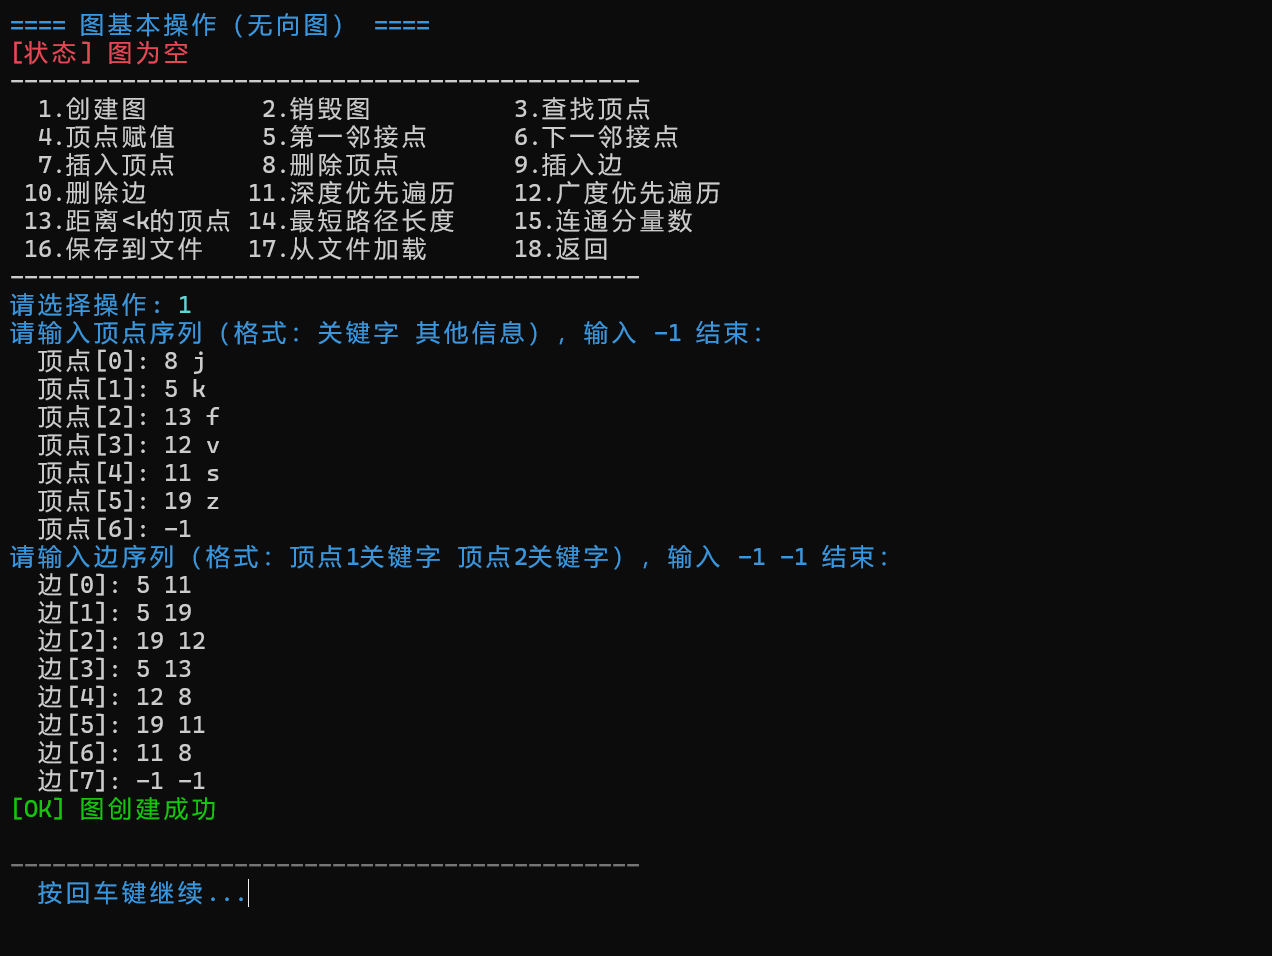
\includegraphics[width=0.75\textwidth]{images/t4_exam4_image6.png}
\caption{向图"江苏"批量插入顶点（关键字1$\sim$8）和边（按图中关系构建邻接表）}
\label{fig:exam4-build-graph}
\end{figure}

\begin{figure}[!htb]
\centering

\includegraphics[width=0.75\textwidth]{images/t4_exam4_image7.png}
\caption{向图"江苏"中追加插入一个新顶点（键为9，值为t），InsertVex追加到vertices末尾}
\label{fig:exam4-insert-vex}
\end{figure}

\begin{figure}[!htb]
\centering
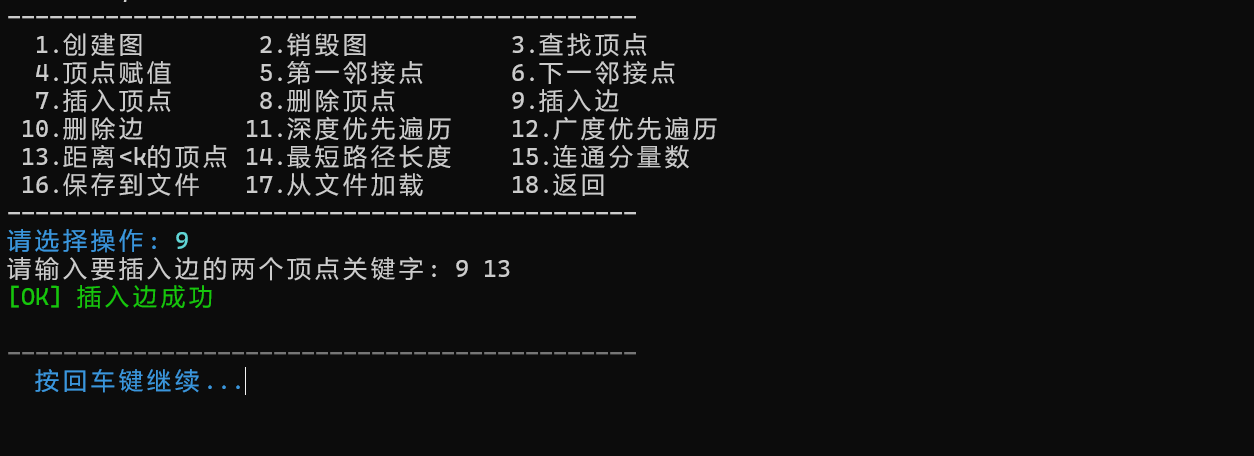
\includegraphics[width=0.75\textwidth]{images/t4_exam4_image14.png}
\caption{向图"江苏"中插入一条边连接结点9:t和13:f，InsertArc头插法双向添加ArcNode}
\label{fig:exam4-insert-arc}
\end{figure}


\begin{figure}[!htb]
\centering
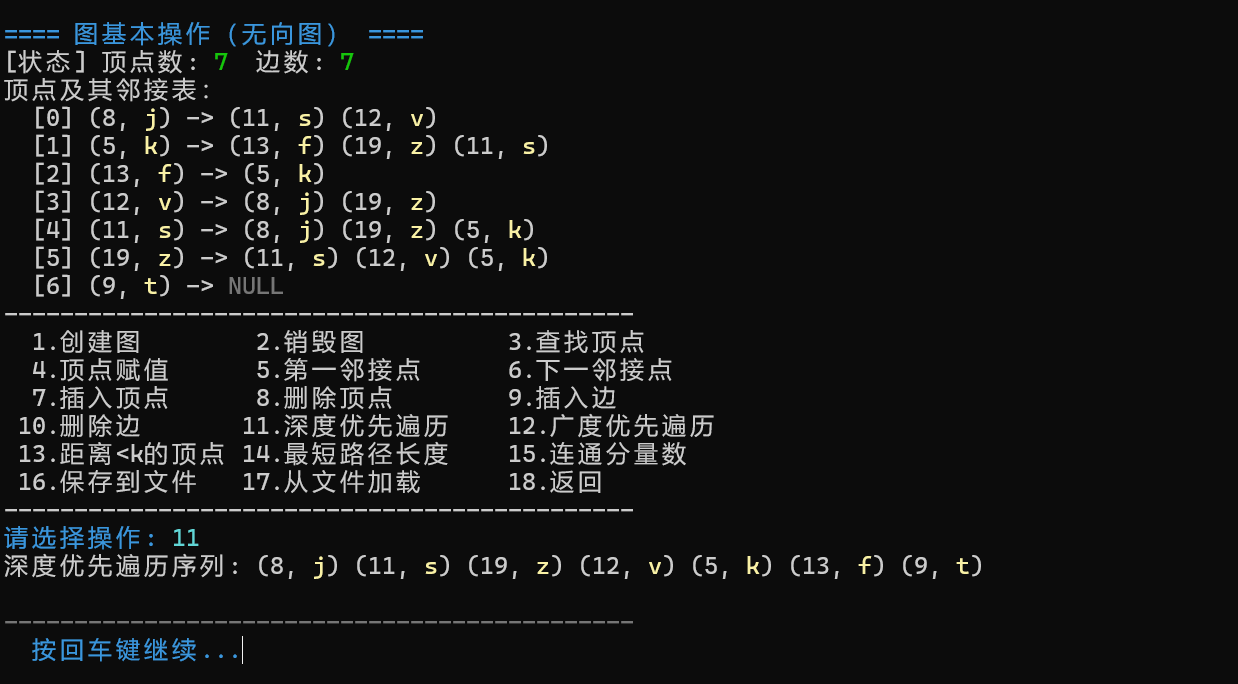
\includegraphics[width=0.75\textwidth]{images/t4_exam4_image8.png}
\caption{对图"江苏"进行DFS深度优先搜索遍历——非递归栈实现，从顶点1出发按深度方向探索}
\label{fig:exam4-dfs}
\end{figure}
\newpage
\begin{figure}[!htb]
\centering
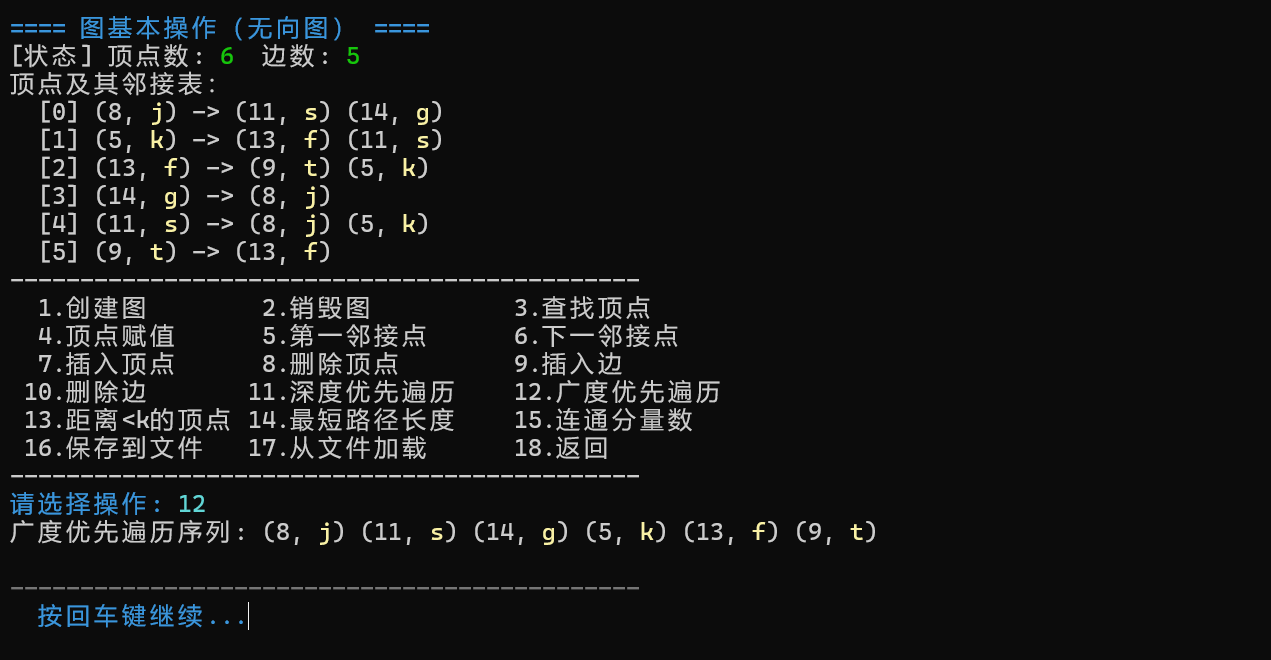
\includegraphics[width=0.75\textwidth]{images/t4_exam4_image16.png}
\caption{对图"江苏"进行BFS广度优先搜索遍历——队列实现，按层逐级展开访问}
\label{fig:exam4-bfs}
\end{figure}


\begin{figure}[!htb]
\centering
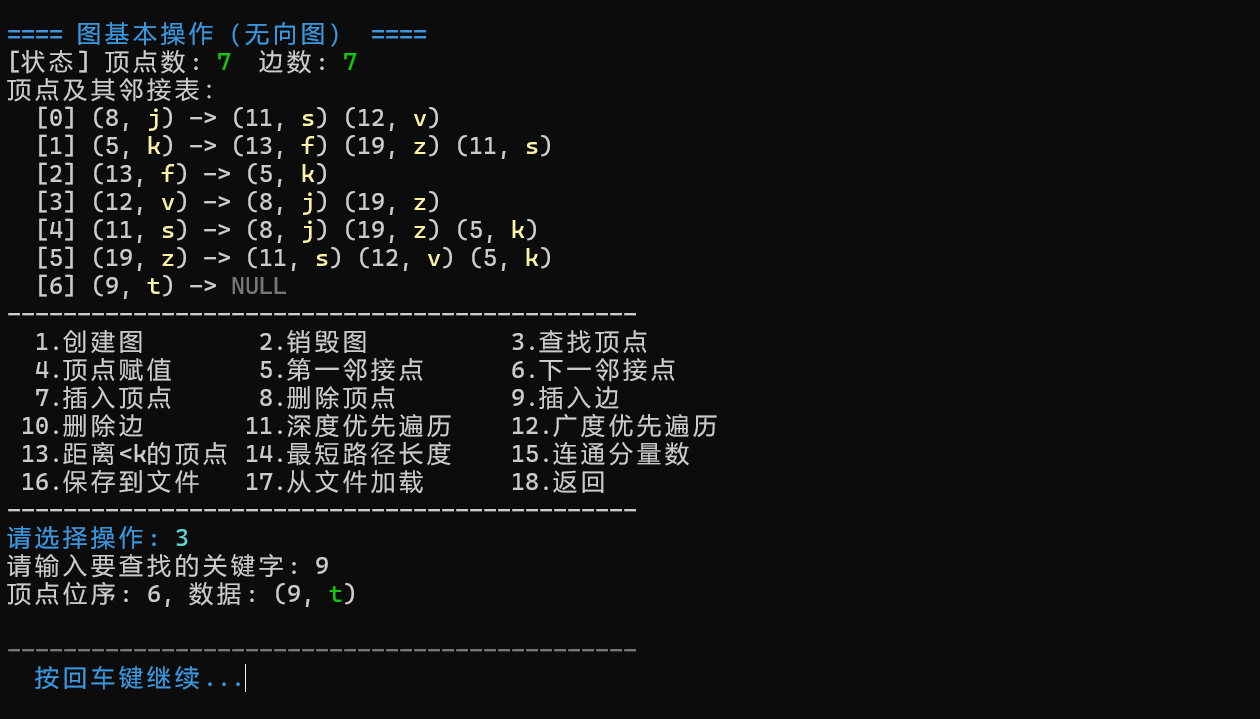
\includegraphics[width=0.75\textwidth]{images/t4_exam4_image9.png}\vspace{2pt}
\caption{查找图"江苏"中键为9的结点——LocateVex返回位序并输出顶点信息（查找键为15的结点失败，显示不存在）}
\label{fig:exam4-locate}
\end{figure}

\begin{figure}[!htb]
\centering

\includegraphics[width=0.75\textwidth]{images/t4_exam4_image10.png}\vspace{2pt}
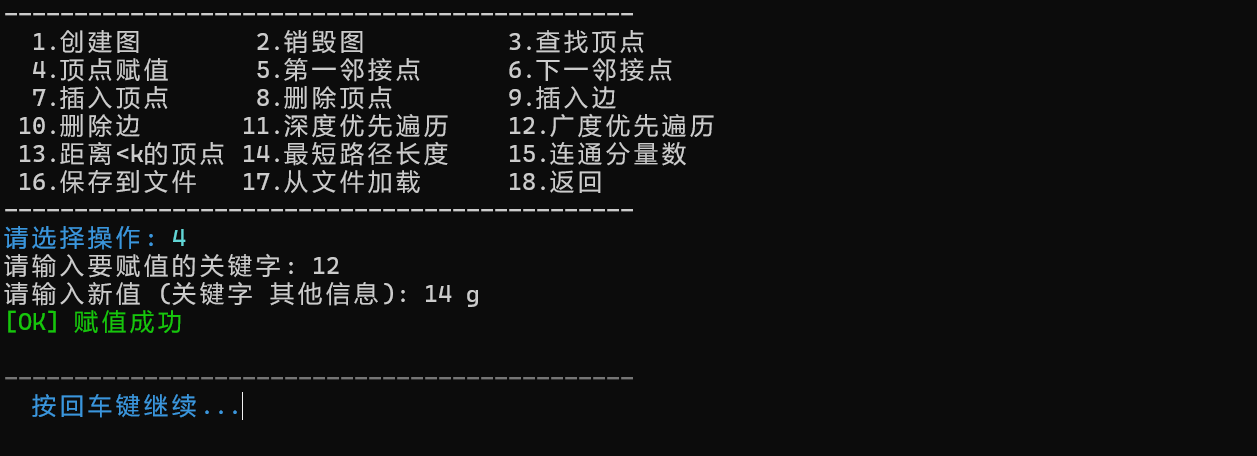
\includegraphics[width=0.75\textwidth]{images/t4_exam4_image11.png}
\caption{PutVex顶点赋值——将键12的顶点键改为14、值改为g，遍历确认修改生效且邻接关系保持}
\label{fig:exam4-putvex}
\end{figure}


\begin{figure}[!htb]
\centering
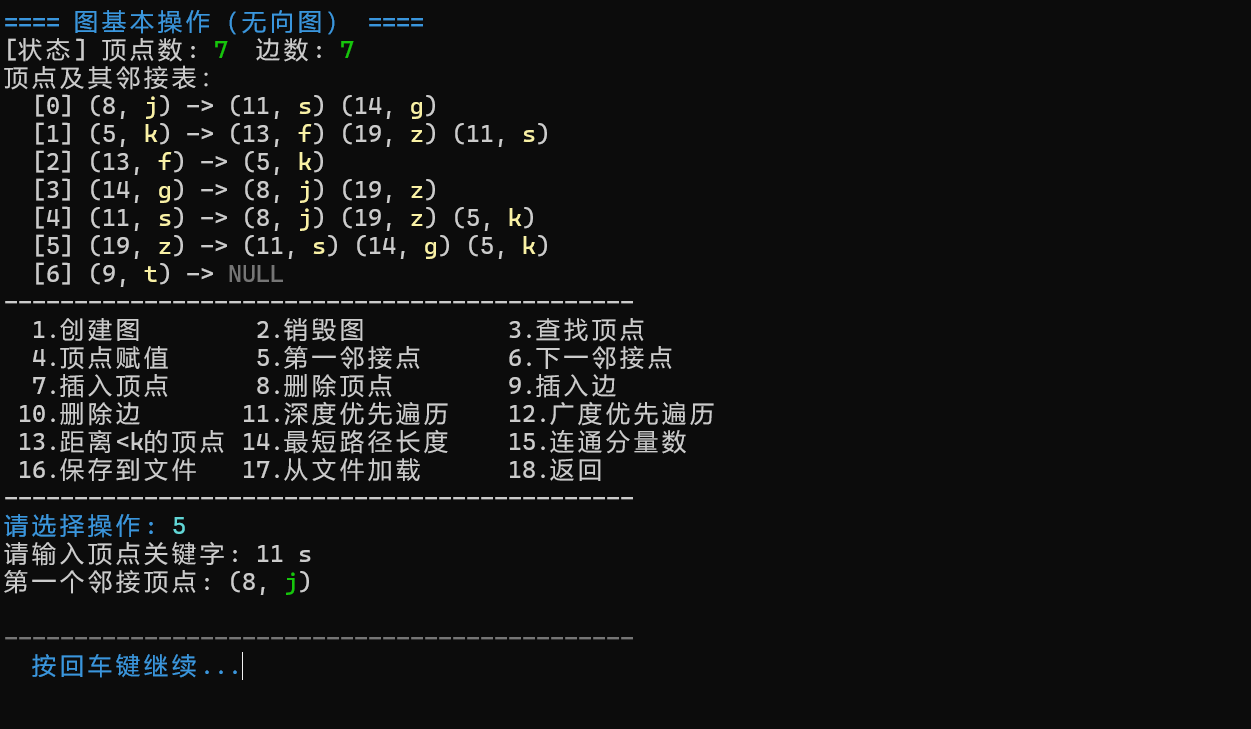
\includegraphics[width=0.75\textwidth]{images/t4_exam4_image12.png}
\caption{FirstAdjVex获取结点11:s的第一个邻接点（19:z），返回其adjvex值}
\label{fig:exam4-firstadj}
\end{figure}

\begin{figure}[!htb]
\centering
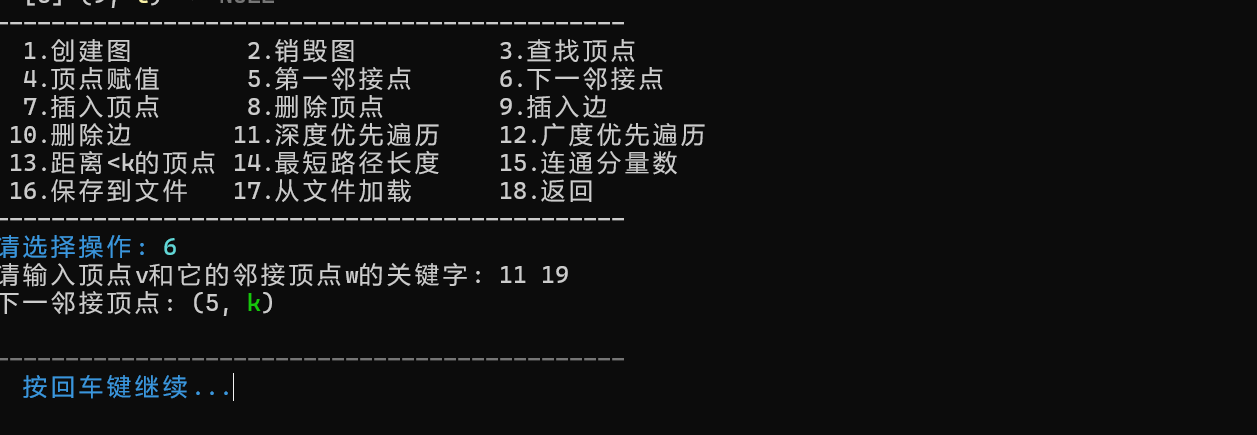
\includegraphics[width=0.75\textwidth]{images/t4_exam4_image13.png}
\caption{NextAdjVex获取结点11:s相对于19:z的下一个邻接点（遍历弧链表找到w后再取后继）}
\label{fig:exam4-nextadj}
\end{figure}


\begin{figure}[!htb]
\centering
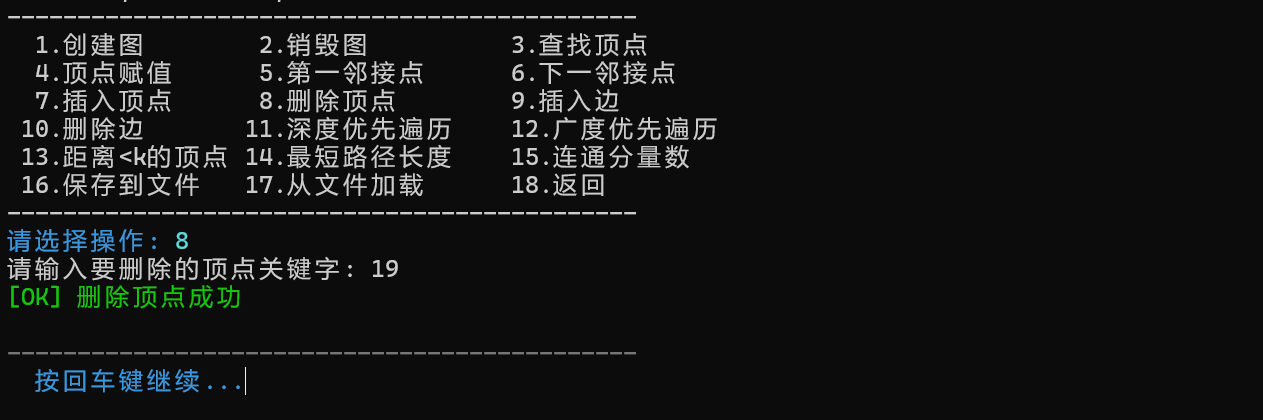
\includegraphics[width=0.75\textwidth]{images/t4_exam4_image15.png}
\caption{DeleteVex四步删除——删除键为19的顶点：统计关联弧→清理其他顶点引用→释放自身弧链→数组前移+adjvex下标校正，遍历验证删除成功}
\label{fig:exam4-delete-vex}
\end{figure}

\begin{figure}[!htb]
\centering
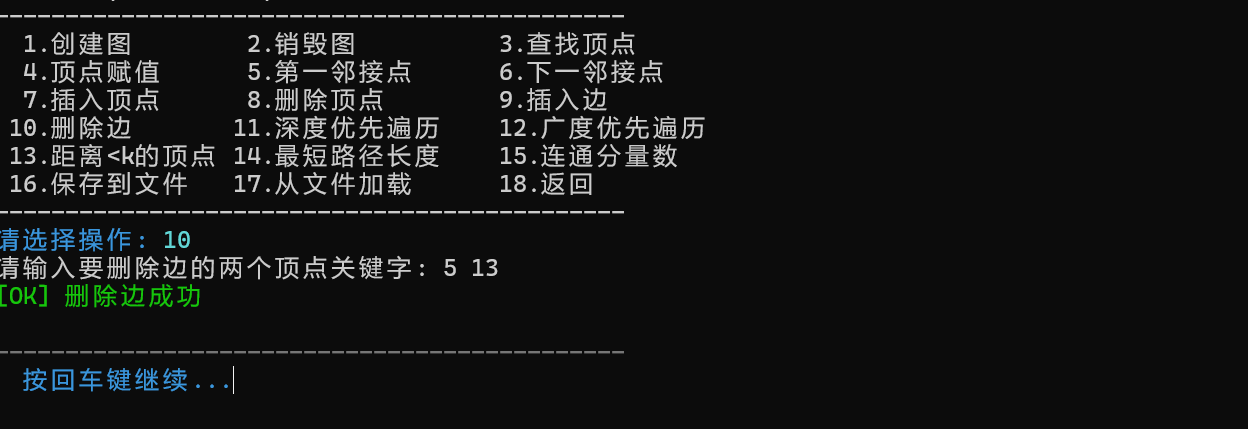
\includegraphics[width=0.75\textwidth]{images/t4_exam4_image17.png}
\caption{DeleteArc删除边(5, 13)——从两端的弧链表中分别定位并删除对应ArcNode（区分头删/中间删），遍历验证邻接表更新正确}
\label{fig:exam4-delete-arc}
\end{figure}


\begin{figure}[!htb]
\centering
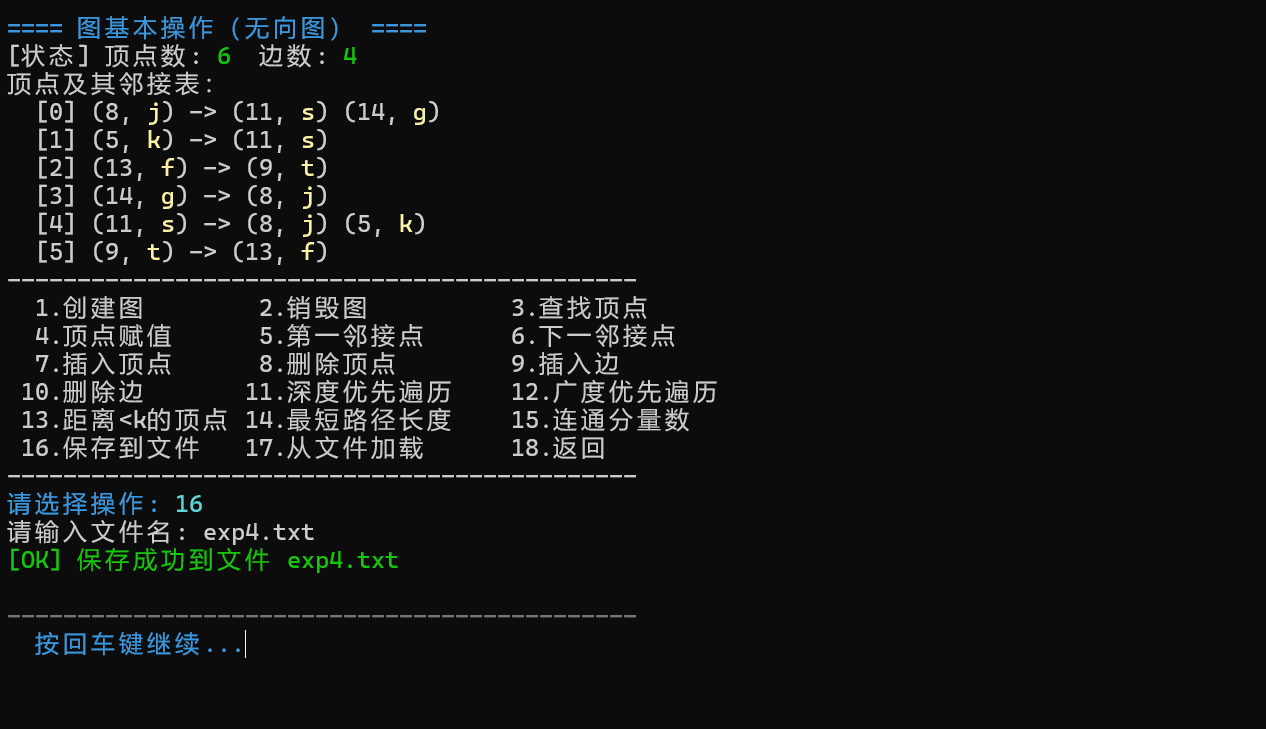
\includegraphics[width=0.75\textwidth]{images/t4_exam4_image18.png}\vspace{2pt}
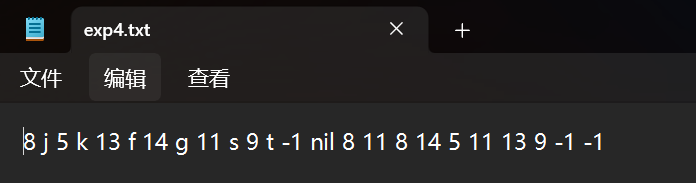
\includegraphics[width=0.75\textwidth]{images/t4_exam4_image19.png}
\caption{将图"江苏"保存至文件 \texttt{exp4.txt}——两段式格式（顶点段+边段），每条边只写一次避免冗余}
\label{fig:exam4-file-save}
\end{figure}

\begin{figure}[!htb]
\centering
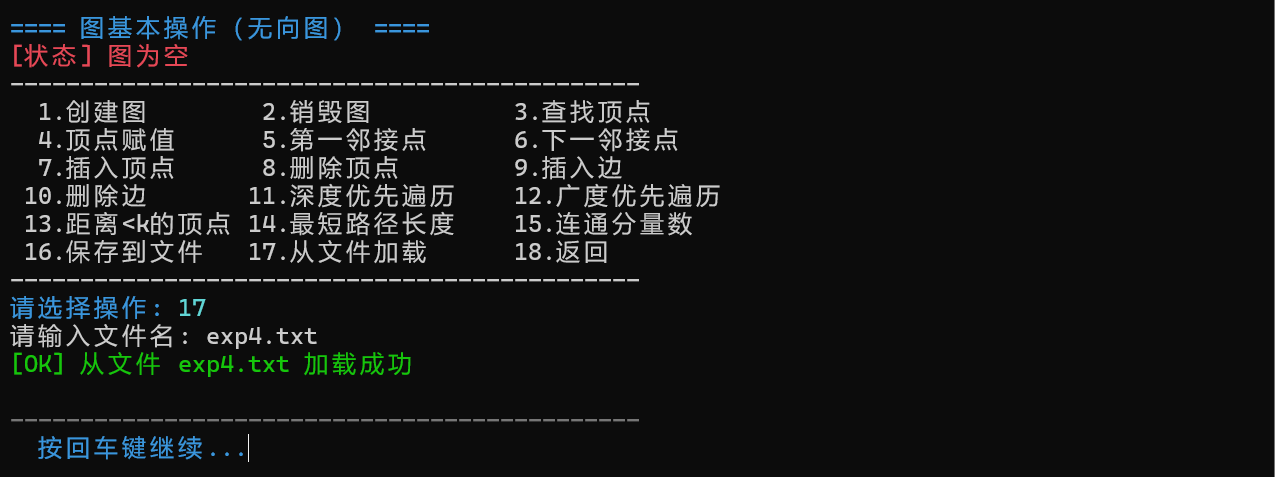
\includegraphics[width=0.75\textwidth]{images/t4_exam4_image22.png}\vspace{2pt}
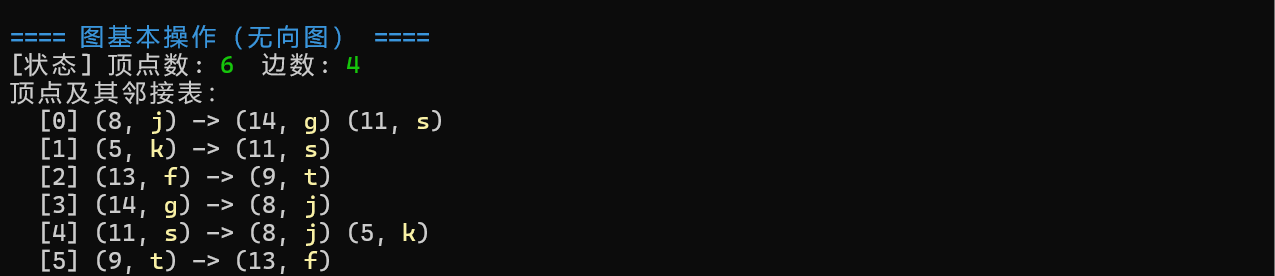
\includegraphics[width=0.75\textwidth]{images/t4_exam4_image23.png}
\caption{图"云南"从文件 \texttt{exp4.txt} 加载数据——先建顶点再补边，恢复邻接表完整结构后遍历}
\label{fig:exam4-file-load}
\end{figure}


\begin{figure}[!htb]
\centering
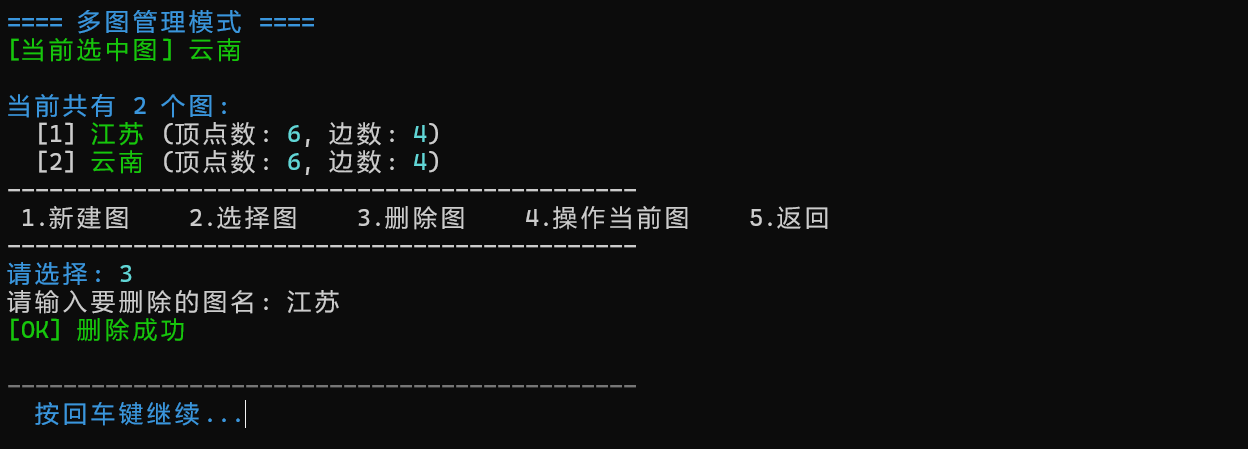
\includegraphics[width=0.75\textwidth]{images/t4_exam4_image24.png}\vspace{2pt}
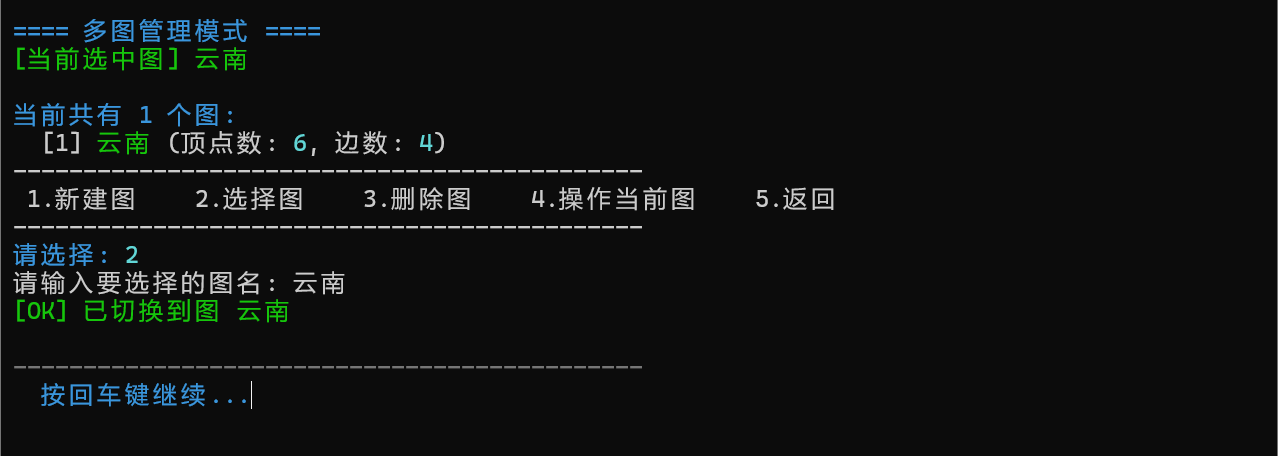
\includegraphics[width=0.75\textwidth]{images/t4_exam4_image25.png}
\caption{多图管理——删除图"江苏"（先DestroyGraph释放全部ArcNode再移除条目）；查找图"云南"的位序}
\label{fig:exam4-multigraph}
\end{figure}


\begin{figure}[!htb]
\centering
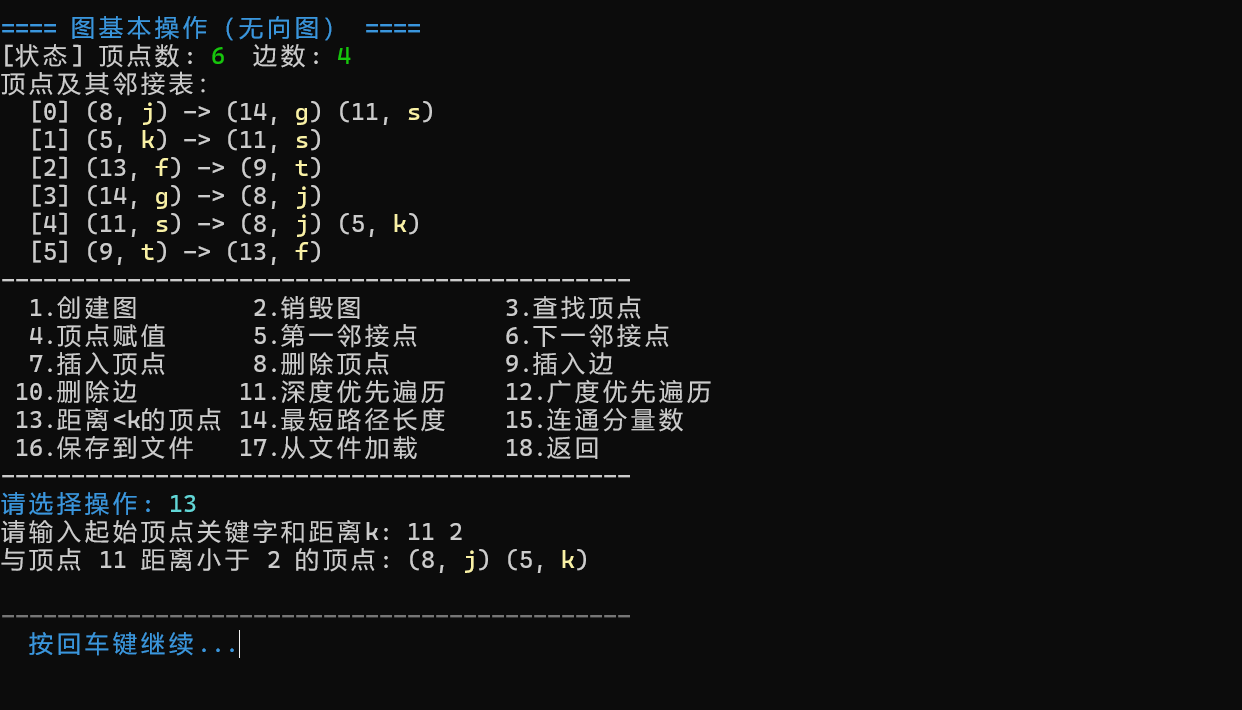
\includegraphics[width=0.75\textwidth]{images/t4_exam4_image26.png}
\caption{VerticesSetLessThanK——查找图"云南"中距离结点11:s小于2的所有顶点（BFS层序遍历截断）}
\label{fig:exam4-lessthank}
\end{figure}
\newpage
\begin{figure}[!htb]
\centering
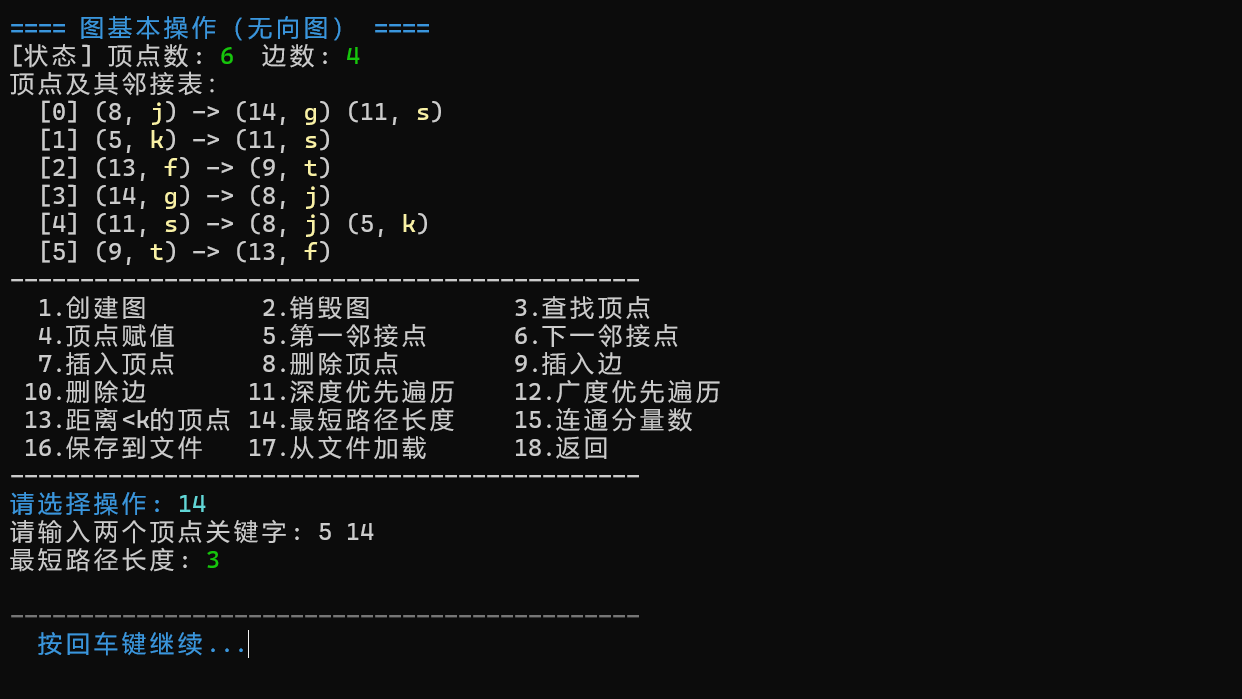
\includegraphics[width=0.75\textwidth]{images/t4_exam4_image27.png}
\caption{ShortestPathLength——计算图"云南"中结点5:k到结点14:g的最短路径长度（BFS首次相遇即最短）}
\label{fig:exam4-shortest}
\end{figure}

\begin{figure}[!htb]
\centering
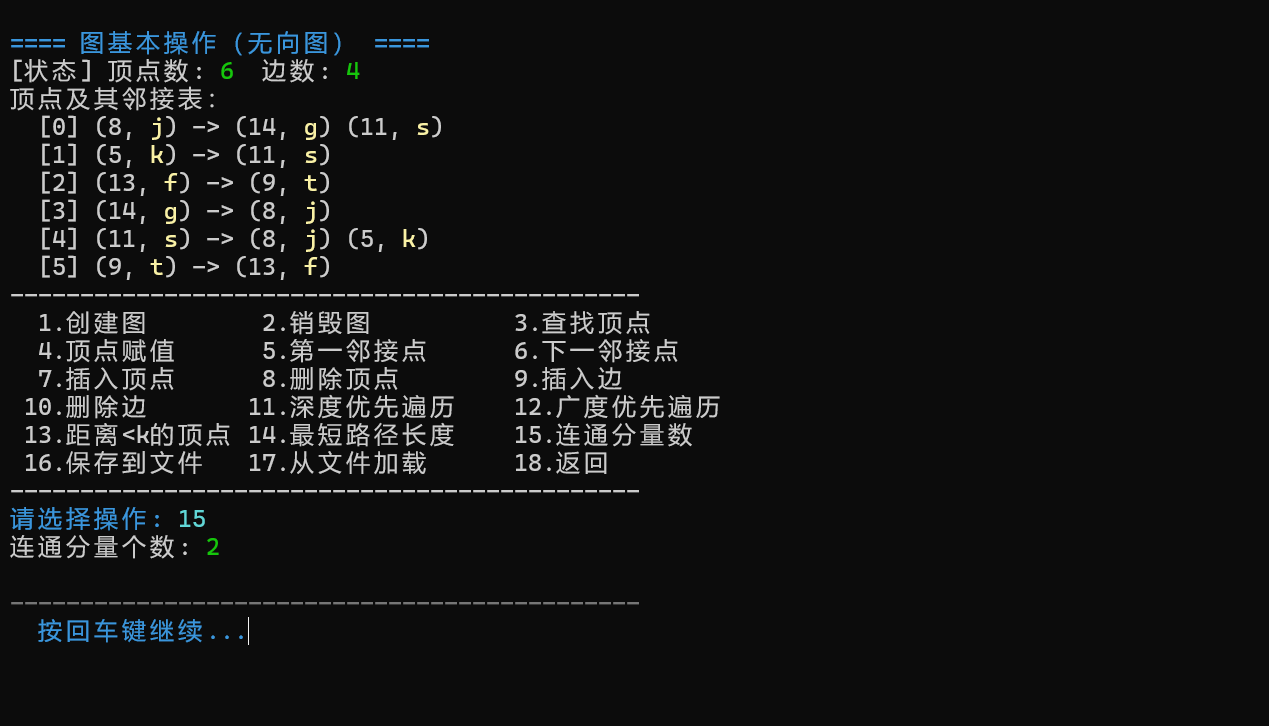
\includegraphics[width=0.75\textwidth]{images/t4_exam4_image28.png}
\caption{ConnectedComponentsNums——计算图"云南"的连通分量数目（BFS外层循环统计visited==0次数）}
\label{fig:exam4-components}
\end{figure}



\newpage

%==========================================================================
\section{总结与反思}
%==========================================================================

通过本次数据结构综合实验，对线性表和图的链式存储结构及算法有了系统性的掌握。

\subsection{实验二（线性表）核心收获}

单链表作为最基础的链式结构，其指针操作构成了后续所有复杂数据结构的基础。头节点（哨兵节点）的设计统一了空表/非空表的操作——"用极小的空间代价换取代码统一性"。逆置（头插法）、插入（搭桥）、删除（绕行）构成三大指针范式，快慢指针法则展示了"双指针同步"思想的广泛适用性。

\subsection{实验四（图）核心收获}

邻接表将链表的应用提升了一个维度——从一维的线性链表升级为二维的"顶点数组+弧链表"结构。DFS的非递归栈实现和BFS的队列实现直观展示了"不同的辅助数据结构导致截然不同的遍历策略"。BFS的三个应用证明了"一种遍历框架可以衍生多种用途"。DeleteVex的下标校正操作蕴含的原理——数组下标作为引用时需要全局维护——在操作系统（文件描述符）、编译器（符号表）、数据库（页号映射）中被反复验证。

\subsection{共性与架构}

两个实验共享了三层架构设计模式（数据层/操作层/交互层）和多对象管理方法（结构体数组+名称索引），这种复用深刻体现了软件架构的价值。内存管理纪律（"每个malloc都有对应free、每条错误路径都妥善清理"）贯穿始终，是C语言编程的基石。

\subsection{不足与展望}

\begin{itemize}
    \item 链表排序$O(n^2)$可升级为归并排序（$O(n\log n)$，天然适合链表拆分合并）
    \item 图系统可扩展有向图、带权图（ArcNode加weight），增加MST、Dijkstra等经典算法
    \item 可封装独立的栈/队列ADT，提高DFS/BFS代码复用性
    \item 可引入CMake整合两个实验为统一的数据结构演示平台
\end{itemize}

\newpage

\begin{thebibliography}{99}
\bibitem{ref1} 袁凌,祝建华,许贵平,李剑军,周全.数据结构——从概念到算法（C语言微课版）.北京:人民邮电出版社,2023.
\end{thebibliography}

\newpage

%==========================================================================
% 附录：完整源代码
%==========================================================================
\section*{附录A\quad 实验一完整源代码}
\addcontentsline{toc}{section}{附录A\quad 实验一完整源代码}
%==========================================================================


\begin{lstlisting}[
    caption={线性表基本操作——完整源代码（实验一代码.cpp）},
    label={lst:exp1-full},
    basicstyle=\ttfamily\fontsize{7}{8}\selectfont,
    numbers=left,
    numberstyle=\tiny\color{modernNumber},
    stepnumber=1,
    numbersep=6pt,
    frame=single,
    framesep=4pt,
    framerule=0.5pt,
    breaklines=true,
    breakatwhitespace=true,
    tabsize=2,
    xleftmargin=6pt,
    xrightmargin=6pt,
    aboveskip=6pt,
    belowskip=6pt
]
#include <stdio.h>
#include <stdlib.h>
#include <string.h>
#include <windows.h>

// ============================================================
// 实验一：线性表基本操作 —— 完整源代码
// 文件名：实验一代码.cpp
// 功能概要：单链表12个基本操作（初始化、销毁、清空、判空、求长、
//           取值、查找、前驱后继、插入、删除、遍历）
//           + 高级操作（逆置、快慢指针删除倒数第N、冒泡排序）
//           + 文件保存/加载 + 多表管理（创建/选择/删除命名表）
// 编程语言：C (C99标准)
// 编译环境：MinGW g++ (Windows)
// ============================================================


#define TRUE 1
#define FALSE 0
#define OK 1
#define ERROR 0
#define INFEASIBLE -1
#define OVERFLOW -2

#define MAX_LIST_NUM 10
#define MAX_NAME_LEN 20

typedef int status;
typedef int ElemType;


typedef struct LNode {
    ElemType data;
    struct LNode *next;
} LNode, *LinkList;

void SetConsoleColor(int color) {
    HANDLE hConsole = GetStdHandle(STD_OUTPUT_HANDLE);
    SetConsoleTextAttribute(hConsole, color);
}

typedef struct {
    char name[MAX_NAME_LEN];
    LinkList L;
} NamedList;

typedef struct {
    NamedList elem[MAX_LIST_NUM];
    int length;
} LISTS;

LISTS lists;     

//-------- 基本操作函数组 --------
status InitList(LinkList *L) {
    if (*L != NULL) return INFEASIBLE;
    LinkList t = (LinkList)malloc(sizeof(LNode));
    if (t == NULL) return OVERFLOW;
    t->next = NULL;
    *L = t;
    return OK;
}

status DestroyList(LinkList *L) {
    if (*L == NULL) return INFEASIBLE;
    LinkList p = *L;
    while (*L != NULL) {
        p = (*L)->next;
        free(*L);
        *L = p;
    }
    *L = NULL;
    return OK;
}

status ClearList(LinkList *L) {
    if (*L == NULL) return INFEASIBLE;
    LinkList p = (*L)->next;
    LinkList q = (*L)->next;
    while (q != NULL) {
        p = q->next;
        free(q);
        q = p;
    }
    (*L)->next = NULL;
    return OK;
}

status ListEmpty(LinkList L) {
    if (L == NULL) return INFEASIBLE;
    return (L->next == NULL) ? TRUE : FALSE;
}

int ListLength(LinkList L) {
    int cnt = 0;
    if (L == NULL) return INFEASIBLE;
    while (L != NULL) {
        cnt++;
        L = L->next;
    }
    return cnt - 1;  
}

status GetElem(LinkList L, int i, ElemType *e) {
    if (L == NULL) return INFEASIBLE;
    if (L->next == NULL) return ERROR;
    int cnt = 0;
    L = L->next;
    while (L != NULL) {
        cnt++;
        if (cnt == i) {
            *e = L->data;
            return OK;
        }
        L = L->next;
    }
    return ERROR;
}

status LocateElem(LinkList L, ElemType e) {
    if (L == NULL) return INFEASIBLE;
    int i = 1;
    L = L->next;
    while (L != NULL) {
        if (L->data == e) return i;
        i++;
        L = L->next;
    }
    return 0;
}

status PriorElem(LinkList L, ElemType e, ElemType *pre) {
    if (L == NULL) return INFEASIBLE;
    if (L->next == NULL || L->next->next == NULL) return ERROR;
    LinkList p = L->next;
    L = L->next->next;
    while (L != NULL) {
        if (L->data == e) {
            *pre = p->data;
            return OK;
        }
        L = L->next;
        p = p->next;
    }
    return ERROR;
}

status NextElem(LinkList L, ElemType e, ElemType *next) {
    if (L == NULL) return INFEASIBLE;
    if (L->next == NULL || L->next->next == NULL) return ERROR;
    LinkList s = L->next;
    L = L->next->next;
    while (L != NULL) {
        if (s->data == e) {
            *next = L->data;
            return OK;
        }
        L = L->next;
        s = s->next;
    }
    return ERROR;
}

status ListInsert(LinkList *L, int i, ElemType e) {
    if (*L == NULL) return INFEASIBLE;
    LinkList p = *L;
    LinkList q = (*L)->next;
    int cnt = 1;
    while (cnt != i && q != NULL) {
        p = p->next;
        q = q->next;
        cnt++;
    }
    if (cnt != i) return ERROR;
    LinkList t = (LinkList)malloc(sizeof(LNode));
    if (t == NULL) return OVERFLOW;
    t->data = e;
    t->next = q;
    p->next = t;
    return OK;
}

status ListDelete(LinkList *L, int i, ElemType *e) {
    if (*L == NULL) return INFEASIBLE;
    if ((*L)->next == NULL) return ERROR;
    LinkList s = *L;
    LinkList f = (*L)->next;
    int cnt = 1;
    while (f != NULL) {
        if (cnt == i) {
            *e = f->data;
            s->next = f->next;
            free(f);
            return OK;
        }
        f = f->next;
        s = s->next;
        cnt++;
    }
    return ERROR;
}

status ListTraverse(LinkList L) {
    if (L == NULL) return INFEASIBLE;
    L = L->next;
    while (L != NULL) {
        SetConsoleColor(14);
        printf("%d", L->data);
        SetConsoleColor(7);
        if (L->next != NULL) printf(" ");
        L = L->next;
    }
    return OK;
}

//-------- 附加功能函数组 --------
status reverseList(LinkList L) {
    if (L == NULL) return INFEASIBLE;
    LinkList p = L->next;
    L->next = NULL;
    while (p != NULL) {
        LinkList q = p->next;
        p->next = L->next;
        L->next = p;
        p = q;
    }
    return OK;
}

status RemoveNthFromEnd(LinkList L, int n) {
    if (L == NULL) return INFEASIBLE;
    if (n <= 0) return ERROR;
    LinkList fast = L->next;
    LinkList slow = L;
    int i;
    for (i = 0; i < n && fast != NULL; i++)
        fast = fast->next;
    if (i < n) return ERROR;
    while (fast != NULL) {
        slow = slow->next;
        fast = fast->next;
    }
    LinkList del = slow->next;
    slow->next = del->next;
    free(del);
    return OK;
}

status sortList(LinkList L) {
    if (L == NULL) return INFEASIBLE;
    if (L->next == NULL || L->next->next == NULL) return OK;
    int len = ListLength(L);
    for (int i = 0; i < len - 1; i++) {
        LinkList q = L->next;
        for (int j = 0; j < len - 1 - i; j++) {
            LinkList p = q->next;
            if (q->data > p->data) {
                ElemType tmp = q->data;
                q->data = p->data;
                p->data = tmp;
            }
            q = q->next;
        }
    }
    return OK;
}

//-------- 文件持久化函数 --------
status SaveList(LinkList L, char FileName[]) {
    if (L == NULL) return INFEASIBLE;
    FILE *fp = fopen(FileName, "w");
    if (fp == NULL) return ERROR;
    LinkList p = L->next;
    while (p != NULL) {
        fprintf(fp, "%d ", p->data);
        p = p->next;
    }
    fclose(fp);
    return OK;
}

status LoadList(LinkList *L, char FileName[]) {
    if (*L != NULL) {
        DestroyList(L);  
    }
    FILE *fp = fopen(FileName, "r");
    if (fp == NULL) return ERROR;
    *L = (LinkList)malloc(sizeof(LNode));
    if (*L == NULL) {
        fclose(fp);
        return OVERFLOW;
    }
    (*L)->next = NULL;
    LinkList tail = *L;
    int data;
    while (fscanf(fp, "%d", &data) != EOF) {
        LinkList newNode = (LinkList)malloc(sizeof(LNode));
        if (newNode == NULL) {
            fclose(fp);
            return OVERFLOW;
        }
        newNode->data = data;
        newNode->next = NULL;
        tail->next = newNode;
        tail = newNode;
    }
    fclose(fp);
    return OK;
}


//多表管理

 
//-------- 多表管理函数组 --------
status AddList(LISTS *Lists, char ListName[]) {
    if (Lists->length >= MAX_LIST_NUM) return ERROR;
    int i = 0;
    while (ListName[i]) {
        Lists->elem[Lists->length].name[i] = ListName[i];
        i++;
    }
    Lists->elem[Lists->length].name[i] = '\0';
    Lists->elem[Lists->length].L = NULL;       
   // InitList(&Lists->elem[Lists->length].L);
    Lists->length++;
    return OK;
}

status RemoveList(LISTS *Lists, char ListName[]) {
    int pos = -1;
    for (int i = 0; i < Lists->length; i++) {
        if (strcmp(Lists->elem[i].name, ListName) == 0) {
            pos = i;
            break;
        }
    }
    if (pos == -1) return ERROR;
    DestroyList(&Lists->elem[pos].L);
    for (int i = pos; i < Lists->length - 1; i++)
        Lists->elem[i] = Lists->elem[i + 1];
    Lists->length--;
    return OK;
}

int LocateList(LISTS Lists, char ListName[]) {
    for (int i = 0; i < Lists.length; i++) {
        if (strcmp(Lists.elem[i].name, ListName) == 0)
            return i + 1;  
    }
    return 0;
}

void ListAllNames(LISTS Lists) {
    SetConsoleColor(3);
    printf("\n当前线性表列表 (%d个)：\n", Lists.length);
    SetConsoleColor(7);
    for (int i = 0; i < Lists.length; i++) {
        printf("  [%d] ", i + 1);
        SetConsoleColor(10);
        printf("%s", Lists.elem[i].name);
        SetConsoleColor(7);
        printf(" (长度:");
        SetConsoleColor(11);
        printf("%d", ListLength(Lists.elem[i].L));
        SetConsoleColor(7);
        printf(")\n");
    }
}

void pressEnter() {
    SetConsoleColor(8);
    printf("\n---------------------------------------------\n");
    SetConsoleColor(3);
    printf("  按回车键继续...");
    SetConsoleColor(7);
    getchar(); while (getchar() != '\n');
}

void printTitle(const char *title) {
    printf("\n");
    SetConsoleColor(3);
    printf("==== %s ====\n", title);
    SetConsoleColor(7);
}

void operateTableMenu(LinkList *L) {
    int op, i;
    ElemType e, pre_e, next_e;
    char filename[50];

    while (1) {
        system("cls");
        printTitle("链式表操作菜单");

        if (*L == NULL) {
            SetConsoleColor(12);
            printf("[状态] 表未初始化，请先初始化\n");
            SetConsoleColor(7);
        } else {
            printf("[状态] 长度：");
            SetConsoleColor(10); printf("%d", ListLength(*L)); SetConsoleColor(7);
            printf("  头结点：存在\n");
            if (ListLength(*L) > 0) {
                printf("[元素] ");
                ListTraverse(*L);
                printf("\n");
            } else {
                SetConsoleColor(8);
                printf("[元素] 空表\n");
                SetConsoleColor(7);
            }
        }

        printf("---------------------------------------------\n");
        printf(" 1.初始化表    7.查找元素    13.翻转链表\n");
        printf(" 2.销毁表      8.获取前驱    14.删除倒数第N个节点\n");
        printf(" 3.清空表      9.获取后继    15.表排序\n");
        printf(" 4.判空       10.插入元素    16.保存到文件\n");
        printf(" 5.求表长     11.删除元素    17.从文件加载\n");
        printf(" 6.获取元素   12.遍历输出    18.返回上级\n");
        printf("---------------------------------------------\n");

        SetConsoleColor(3);
        printf("请选择操作：");
        SetConsoleColor(11);
        scanf("%d", &op);
        SetConsoleColor(7);

        switch (op) {
            case 1:
                if (InitList(L) == OK) {
                    SetConsoleColor(10); printf("[OK] 初始化成功！\n"); SetConsoleColor(7);
                } else {
                    SetConsoleColor(12); printf("[FAIL] 初始化失败，表已存在！\n"); SetConsoleColor(7);
                }
                break;
            case 2:
                if (DestroyList(L) == OK) {
                    SetConsoleColor(10); printf("[OK] 销毁成功！\n"); SetConsoleColor(7);
                } else {
                    SetConsoleColor(12); printf("[FAIL] 销毁失败，表不存在！\n"); SetConsoleColor(7);
                }
                break;
            case 3:
                if (ClearList(L) == OK) {
                    SetConsoleColor(10); printf("[OK] 清空成功！\n"); SetConsoleColor(7);
                } else {
                    SetConsoleColor(12); printf("[FAIL] 清空失败！\n"); SetConsoleColor(7);
                }
                break;
            case 4: {
                int ret = ListEmpty(*L);
                if (ret == INFEASIBLE) {
                    SetConsoleColor(12); printf("[FAIL] 表不存在！\n"); SetConsoleColor(7);
                } else {
                    printf("表%s空\n", ret == TRUE ? "为" : "不为");
                }
                break;
            }
            case 5: {
                int len = ListLength(*L);
                if (len == INFEASIBLE) {
                    SetConsoleColor(12); printf("[FAIL] 表不存在！\n"); SetConsoleColor(7);
                } else {
                    printf("表长：%d\n", len);
                }
                break;
            }
            case 6:
                printf("输入位置i：");
                scanf("%d", &i);
                if (GetElem(*L, i, &e) == OK) {
                    printf("第%d个元素：%d\n", i, e);
                } else {
                    SetConsoleColor(12); printf("[FAIL] 获取失败！\n"); SetConsoleColor(7);
                }
                break;
            case 7:
                printf("输入查找值：");
                scanf("%d", &e);
                i = LocateElem(*L, e);
                if (i == INFEASIBLE) {
                    SetConsoleColor(12); printf("[FAIL] 表不存在！\n"); SetConsoleColor(7);
                } else if (i == 0) {
                    printf("未找到该元素\n");
                } else {
                    printf("元素位于第 %d 位\n", i);
                }
                break;
            case 8:
                printf("输入当前元素：");
                scanf("%d", &e);
                if (PriorElem(*L, e, &pre_e) == OK) {
                    printf("前驱值：%d\n", pre_e);
                } else {
                    SetConsoleColor(12); printf("[FAIL] 无此元素或无前驱\n"); SetConsoleColor(7);
                }
                break;
            case 9:
                printf("输入当前元素：");
                scanf("%d", &e);
                if (NextElem(*L, e, &next_e) == OK) {
                    printf("后继值：%d\n", next_e);
                } else {
                    SetConsoleColor(12); printf("[FAIL] 无此元素或无后继\n"); SetConsoleColor(7);
                }
                break;
            case 10:
                printf("输入位置i 和 值e：");
                scanf("%d %d", &i, &e);
                if (ListInsert(L, i, e) == OK) {
                    SetConsoleColor(10); printf("[OK] 插入成功！\n"); SetConsoleColor(7);
                } else {
                    SetConsoleColor(12); printf("[FAIL] 插入失败！\n"); SetConsoleColor(7);
                }
                break;
            case 11:
                printf("输入删除位置i：");
                scanf("%d", &i);
                if (ListDelete(L, i, &e) == OK) {
                    SetConsoleColor(10); printf("[OK] 删除成功，值：%d\n", e); SetConsoleColor(7);
                } else {
                    SetConsoleColor(12); printf("[FAIL] 删除失败！\n"); SetConsoleColor(7);
                }
                break;
            case 12:
                if (ListTraverse(*L) == INFEASIBLE) {
                    SetConsoleColor(12); printf("[FAIL] 表不存在！\n"); SetConsoleColor(7);
                } else {
                    printf("\n遍历完成\n");
                }
                break;
            case 13:
                if (reverseList(*L) == OK) {
                    SetConsoleColor(10); printf("[OK] 链表已翻转\n"); SetConsoleColor(7);
                } else {
                    SetConsoleColor(12); printf("[FAIL] 翻转失败\n"); SetConsoleColor(7);
                }
                break;
            case 14:
                printf("输入倒数第N个节点：");
                scanf("%d", &i);
                if (RemoveNthFromEnd(*L, i) == OK) {
                    SetConsoleColor(10); printf("[OK] 删除成功\n"); SetConsoleColor(7);
                } else {
                    SetConsoleColor(12); printf("[FAIL] 删除失败 (n非法或表为空)\n"); SetConsoleColor(7);
                }
                break;
            case 15:
                if (sortList(*L) == OK) {
                    SetConsoleColor(10); printf("[OK] 排序完成（升序）\n"); SetConsoleColor(7);
                } else {
                    SetConsoleColor(12); printf("[FAIL] 排序失败\n"); SetConsoleColor(7);
                }
                break;
            case 16:
                printf("输入保存文件名：");
                scanf("%s", filename);
                if (SaveList(*L, filename) == OK) {
                    SetConsoleColor(10); printf("[OK] 保存成功！\n"); SetConsoleColor(7);
                } else {
                    SetConsoleColor(12); printf("[FAIL] 保存失败！\n"); SetConsoleColor(7);
                }
                break;
            case 17:
                printf("输入加载文件名：");
                scanf("%s", filename);
                if (LoadList(L, filename) == OK) {
                    SetConsoleColor(10); printf("[OK] 加载成功！\n"); SetConsoleColor(7);
                } else {
                    SetConsoleColor(12); printf("[FAIL] 加载失败！\n"); SetConsoleColor(7);
                }
                break;
            case 18:
                return;
            default:
                SetConsoleColor(12); printf("[FAIL] 无效选项！\n"); SetConsoleColor(7);
        }
        pressEnter();
    }
}

void singleTableMode() {
    LinkList L = NULL;
    InitList(&L);   
    operateTableMenu(&L);
    DestroyList(&L);
}

//-------- 多表交互控制 --------
void multiTableMode() {
    int op, idx;
    char name[MAX_NAME_LEN];
    int currentIdx = -1;

    while (1) {
        system("cls");
        printTitle("多表管理模式");

        if (currentIdx != -1) {
            SetConsoleColor(10);
            printf("[当前操作表] %s\n", lists.elem[currentIdx].name);
            SetConsoleColor(7);
        } else {
            SetConsoleColor(8);
            printf("[当前操作表] 未选择\n");
            SetConsoleColor(7);
        }

        ListAllNames(lists);
        printf("---------------------------------------------\n");
        printf(" 1.新建表    2.选择表    3.删除表    4.操作当前表    5.返回主菜单\n");
        printf("---------------------------------------------\n");

        SetConsoleColor(3);
        printf("请选择：");
        SetConsoleColor(11);
        scanf("%d", &op);
        SetConsoleColor(7);

        switch (op) {
            case 1:
                printf("输入表名：");
                scanf("%s", name);
                if (AddList(&lists, name) == OK) {
                    SetConsoleColor(10); printf("[OK] 表 \"%s\" 创建成功！\n", name); SetConsoleColor(7);
                } else {
                    SetConsoleColor(12); printf("[FAIL] 创建失败（表名重复或数量已达上限）！\n"); SetConsoleColor(7);
                }
                break;
            case 2:
                printf("输入表名：");
                scanf("%s", name);
                idx = LocateList(lists, name);
                if (idx) {
                    currentIdx = idx - 1;
                    SetConsoleColor(10); printf("[OK] 已切换至表：%s\n", name); SetConsoleColor(7);
                } else {
                    SetConsoleColor(12); printf("[FAIL] 表不存在！\n"); SetConsoleColor(7);
                }
                break;
            case 3:
                printf("输入要删除的表名：");
                scanf("%s", name);
                if (RemoveList(&lists, name) == OK) {
                    if (currentIdx != -1 && strcmp(lists.elem[currentIdx].name, name) == 0)
                        currentIdx = -1;
                    SetConsoleColor(10); printf("[OK] 删除成功！\n"); SetConsoleColor(7);
                } else {
                    SetConsoleColor(12); printf("[FAIL] 删除失败！\n"); SetConsoleColor(7);
                }
                break;
            case 4:
                if (currentIdx == -1) {
                    SetConsoleColor(12); printf("[FAIL] 请先选择表！\n"); SetConsoleColor(7);
                } else {
                    operateTableMenu(&lists.elem[currentIdx].L);
                }
                break;
            case 5:
                return;
            default:
                SetConsoleColor(12); printf("[FAIL] 无效选项！\n"); SetConsoleColor(7);
        }
        pressEnter();
    }
}

//-------- 主函数入口 --------
int main() {
    int op;
    lists.length = 0;

    while (1) {
        system("cls");
        printf("\n");
        SetConsoleColor(3);
        printf("==== 链式线性表综合管理系统 ====\n");
        SetConsoleColor(7);
        printf("\n");
        printf("  1. 单表操作模式\n");
        printf("  2. 多表管理模式\n");
        printf("  0. 退出系统\n");
        printf("\n");
        SetConsoleColor(3);
        printf("请输入功能编号：");
        SetConsoleColor(11);
        scanf("%d", &op);
        SetConsoleColor(7);

        switch (op) {
            case 1:
                singleTableMode();
                break;
            case 2:
                multiTableMode();
                break;
            case 0:
                
                for (int i = 0; i < lists.length; i++) {
                    DestroyList(&lists.elem[i].L);
                }
                SetConsoleColor(10);
                printf("\n感谢使用，再见！\n\n");
                SetConsoleColor(7);
                return 0;
            default:
                SetConsoleColor(12);
                printf("无效选项！\n");
                SetConsoleColor(7);
                pressEnter();
        }
    }
    return 0;
}

\end{lstlisting}

\newpage

\section*{附录B\quad 实验二完整源代码}
\addcontentsline{toc}{section}{附录B\quad 实验二完整源代码}
%==========================================================================


\begin{lstlisting}[
    caption={线性表综合管理系统——完整源代码（exam2.cpp）},
    label={lst:exp2-full},
    basicstyle=\ttfamily\fontsize{7}{8}\selectfont,
    numbers=left,
    numberstyle=\tiny\color{modernNumber},
    stepnumber=1,
    numbersep=6pt,
    frame=single,
    framesep=4pt,
    framerule=0.5pt,
    breaklines=true,
    breakatwhitespace=true,
    tabsize=2,
    xleftmargin=6pt,
    xrightmargin=6pt,
    aboveskip=6pt,
    belowskip=6pt
]
#include <stdio.h>
#include <stdlib.h>
#include <string.h>
#include <windows.h>

// ============================================================
// 线性表综合管理系统  --  完整源代码
// 功能概要：单链表12个基本操作 + 逆置/快慢指针删除/冒泡排序
//          + 文件保存加载 + 多表管理模式
// ============================================================

#define TRUE 1
#define FALSE 0
#define OK 1
#define ERROR 0
#define INFEASIBLE -1
#define OVERFLOW -2

// ---- 容量限制 ----
#define MAX_LIST_NUM 10
#define MAX_NAME_LEN 20

typedef int status;
typedef int ElemType;

// ---- 核心数据结构：单链表节点 ----
typedef struct LNode {
    ElemType data;
    struct LNode *next;
} LNode, *LinkList;

void SetConsoleColor(int color) {
    HANDLE hConsole = GetStdHandle(STD_OUTPUT_HANDLE);
    SetConsoleTextAttribute(hConsole, color);
}

typedef struct {
    char name[MAX_NAME_LEN];
    LinkList L;
} NamedList;

typedef struct {
    NamedList elem[MAX_LIST_NUM];
    int length;
} LISTS;

LISTS lists;

// ============================================================
// 一、单链表基本操作（12个函数）
// 均采用带头节点的单链表实现，头节点不存储数据
// ============================================================
status InitList(LinkList *L) {
    if (*L != NULL) return INFEASIBLE;
    LinkList t = (LinkList)malloc(sizeof(LNode));
    if (t == NULL) return OVERFLOW;
    t->next = NULL;
    *L = t;
    return OK;
}

status DestroyList(LinkList *L) {
    if (*L == NULL) return INFEASIBLE;
    LinkList p = *L;
    while (*L != NULL) {
        p = (*L)->next;
        free(*L);
        *L = p;
    }
    *L = NULL;
    return OK;
}

status ClearList(LinkList *L) {
    if (*L == NULL) return INFEASIBLE;
    LinkList p = (*L)->next;
    LinkList q = (*L)->next;
    while (q != NULL) {
        p = q->next;
        free(q);
        q = p;
    }
    (*L)->next = NULL;
    return OK;
}

status ListEmpty(LinkList L) {
    if (L == NULL) return INFEASIBLE;
    return (L->next == NULL) ? TRUE : FALSE;
}

int ListLength(LinkList L) {
    int cnt = 0;
    if (L == NULL) return INFEASIBLE;
    while (L != NULL) {
        cnt++;
        L = L->next;
    }
    return cnt - 1;
}

status GetElem(LinkList L, int i, ElemType *e) {
    if (L == NULL) return INFEASIBLE;
    if (L->next == NULL) return ERROR;
    int cnt = 0;
    L = L->next;
    while (L != NULL) {
        cnt++;
        if (cnt == i) {
            *e = L->data;
            return OK;
        }
        L = L->next;
    }
    return ERROR;
}

status LocateElem(LinkList L, ElemType e) {
    if (L == NULL) return INFEASIBLE;
    int i = 1;
    L = L->next;
    while (L != NULL) {
        if (L->data == e) return i;
        i++;
        L = L->next;
    }
    return 0;
}

status PriorElem(LinkList L, ElemType e, ElemType *pre) {
    if (L == NULL) return INFEASIBLE;
    if (L->next == NULL || L->next->next == NULL) return ERROR;
    LinkList p = L->next;
    L = L->next->next;
    while (L != NULL) {
        if (L->data == e) {
            *pre = p->data;
            return OK;
        }
        L = L->next;
        p = p->next;
    }
    return ERROR;
}

status NextElem(LinkList L, ElemType e, ElemType *next) {
    if (L == NULL) return INFEASIBLE;
    if (L->next == NULL || L->next->next == NULL) return ERROR;
    LinkList s = L->next;
    L = L->next->next;
    while (L != NULL) {
        if (s->data == e) {
            *next = L->data;
            return OK;
        }
        L = L->next;
        s = s->next;
    }
    return ERROR;
}

status ListInsert(LinkList *L, int i, ElemType e) {
    if (*L == NULL) return INFEASIBLE;
    LinkList p = *L;
    LinkList q = (*L)->next;
    int cnt = 1;
    while (cnt != i && q != NULL) {
        p = p->next;
        q = q->next;
        cnt++;
    }
    if (cnt != i) return ERROR;
    LinkList t = (LinkList)malloc(sizeof(LNode));
    if (t == NULL) return OVERFLOW;
    t->data = e;
    t->next = q;
    p->next = t;
    return OK;
}

status ListDelete(LinkList *L, int i, ElemType *e) {
    if (*L == NULL) return INFEASIBLE;
    if ((*L)->next == NULL) return ERROR;
    LinkList s = *L;
    LinkList f = (*L)->next;
    int cnt = 1;
    while (f != NULL) {
        if (cnt == i) {
            *e = f->data;
            s->next = f->next;
            free(f);
            return OK;
        }
        f = f->next;
        s = s->next;
        cnt++;
    }
    return ERROR;
}

status ListTraverse(LinkList L) {
    if (L == NULL) return INFEASIBLE;
    L = L->next;
    while (L != NULL) {
        SetConsoleColor(14);
        printf("%d", L->data);
        SetConsoleColor(7);
        if (L->next != NULL) printf(" ");
        L = L->next;
    }
    return OK;
}

// ============================================================
// 二、附加功能
// reverseList: 头插法逆置，原地反转 O(n)
// RemoveNthFromEnd: 快慢指针法，一次遍历 O(n)
// sortList: 冒泡排序（交换数据域），O(n^2)
// SaveList/LoadList: 文件持久化
// ============================================================
status reverseList(LinkList L) {
    if (L == NULL) return INFEASIBLE;
    LinkList p = L->next;
    L->next = NULL;                        // 断开链表，逐个节点重新头插
    while (p != NULL) {
        LinkList q = p->next;
        p->next = L->next;
        L->next = p;
        p = q;
    }
    return OK;
}

// 快慢指针法：fast先走n步，然后同步移动
// slow从头节点出发，保证fast到NULL时slow恰为前驱
status RemoveNthFromEnd(LinkList L, int n) {
    if (L == NULL) return INFEASIBLE;
    if (n <= 0) return ERROR;
    LinkList fast = L->next;
    LinkList slow = L;
    int i;
    for (i = 0; i < n && fast != NULL; i++)
        fast = fast->next;
    if (i < n) return ERROR;
    while (fast != NULL) {
        slow = slow->next;
        fast = fast->next;
    }
    LinkList del = slow->next;
    slow->next = del->next;
    free(del);
    return OK;
}

status sortList(LinkList L) {
    if (L == NULL) return INFEASIBLE;
    if (L->next == NULL || L->next->next == NULL) return OK;
    int len = ListLength(L);
    for (int i = 0; i < len - 1; i++) {
        LinkList q = L->next;
        for (int j = 0; j < len - 1 - i; j++) {
            LinkList p = q->next;
            if (q->data > p->data) {
                ElemType tmp = q->data;
                q->data = p->data;
                p->data = tmp;
            }
            q = q->next;
        }
    }
    return OK;
}

status SaveList(LinkList L, char FileName[]) {
    if (L == NULL) return INFEASIBLE;
    FILE *fp = fopen(FileName, "w");
    if (fp == NULL) return ERROR;
    LinkList p = L->next;
    while (p != NULL) {
        fprintf(fp, "%d ", p->data);
        p = p->next;
    }
    fclose(fp);
    return OK;
}

status LoadList(LinkList *L, char FileName[]) {
    if (*L != NULL) {
        DestroyList(L);
    }
    FILE *fp = fopen(FileName, "r");
    if (fp == NULL) return ERROR;
    *L = (LinkList)malloc(sizeof(LNode));
    if (*L == NULL) {
        fclose(fp);
        return OVERFLOW;
    }
    (*L)->next = NULL;
    LinkList tail = *L;
    int data;
    while (fscanf(fp, "%d", &data) != EOF) {
        LinkList newNode = (LinkList)malloc(sizeof(LNode));
        if (newNode == NULL) {
            fclose(fp);
            return OVERFLOW;
        }
        newNode->data = data;
        newNode->next = NULL;
        tail->next = newNode;
        tail = newNode;
    }
    fclose(fp);
    return OK;
}

// ============================================================
// 三、多表管理（LISTS 容器 = 结构体数组 + length 计数）
// AddList: 尾部追加槽位，L初始为NULL（不自动InitList）
// RemoveList: 按名删除，先DestroyList释放节点再数组前移（顺序关键）
// LocateList: 返回1-based序号，0表示不存在
// ============================================================
status AddList(LISTS *Lists, char ListName[]) {
    if (Lists->length >= MAX_LIST_NUM) return ERROR;
    int i = 0;
    while (ListName[i]) {
        Lists->elem[Lists->length].name[i] = ListName[i];
        i++;
    }
    Lists->elem[Lists->length].name[i] = '\0';
    Lists->elem[Lists->length].L = NULL;

    Lists->length++;
    return OK;
}

status RemoveList(LISTS *Lists, char ListName[]) {
    int pos = -1;
    for (int i = 0; i < Lists->length; i++) {
        if (strcmp(Lists->elem[i].name, ListName) == 0) {
            pos = i;
            break;
        }
    }
    if (pos == -1) return ERROR;
    DestroyList(&Lists->elem[pos].L);
    for (int i = pos; i < Lists->length - 1; i++)
        Lists->elem[i] = Lists->elem[i + 1];
    Lists->length--;
    return OK;
}

int LocateList(LISTS Lists, char ListName[]) {
    for (int i = 0; i < Lists.length; i++) {
        if (strcmp(Lists.elem[i].name, ListName) == 0)
            return i + 1;
    }
    return 0;
}

void ListAllNames(LISTS Lists) {
    SetConsoleColor(3);
    printf("\n 当前线性表列表 (%d 个):\n", Lists.length);
    SetConsoleColor(7);
    for (int i = 0; i < Lists.length; i++) {
        printf("  [%d] ", i + 1);
        SetConsoleColor(10);
        printf("%s", Lists.elem[i].name);
        SetConsoleColor(7);
        printf(" (长度:");
        SetConsoleColor(11);
        printf("%d", ListLength(Lists.elem[i].L));
        SetConsoleColor(7);
        printf(")\n");
    }
}

void pressEnter() {
    SetConsoleColor(8);
    printf("\n---------------------------------------------\n");
    SetConsoleColor(3);
    printf("  按回车键继续...");
    SetConsoleColor(7);
    getchar(); while (getchar() != '\n');
}

void printTitle(const char *title) {
    printf("\n");
    SetConsoleColor(3);
    printf("==== %s ====\n", title);
    SetConsoleColor(7);
}

// ============================================================
// 四、交互层 -- 命令行菜单驱动
// operateTableMenu: 单表18项操作菜单 (命令分发器模式)
// singleTableMode: 创建临时表 → 进入菜单 → 退出时销毁
// multiTableMode: 多表管理交互 (新建/选择/删除/操作当前表)
// pressEnter / printTitle / SetConsoleColor: 控制台辅助
// ============================================================
void operateTableMenu(LinkList *L) {
    int op, i;
    ElemType e, pre_e, next_e;
    char filename[50];

    while (1) {
        system("cls");
        printTitle("线性表操作菜单");

        if (*L == NULL) {
            SetConsoleColor(12);
            printf("[状态] 表未初始化，请先初始化\n");
            SetConsoleColor(7);
        } else {
            printf("[状态] 长度：");
            SetConsoleColor(10); printf("%d", ListLength(*L)); SetConsoleColor(7);
            printf("  头结点：存在\n");
            if (ListLength(*L) > 0) {
                printf("[元素] ");
                ListTraverse(*L);
                printf("\n");
            } else {
                SetConsoleColor(8);
                printf("[元素] 空表\n");
                SetConsoleColor(7);
            }
        }

        printf("---------------------------------------------\n");
        printf(" 1.初始化表    7.定位元素    13.逆置链表\n");
        printf(" 2.销毁表      8.获取前驱    14.删除倒数第N个节点\n");
        printf(" 3.清空表      9.获取后继    15.排序\n");
        printf(" 4.判空       10.插入元素    16.保存到文件\n");
        printf(" 5.求长度     11.删除元素    17.从文件加载\n");
        printf(" 6.获取元素   12.遍历输出    18.返回上级\n");
        printf("---------------------------------------------\n");

        SetConsoleColor(3);
        printf("请选择操作：");
        SetConsoleColor(11);
        scanf("%d", &op);
        SetConsoleColor(7);

        switch (op) {
            case 1:
                if (InitList(L) == OK) {
                    SetConsoleColor(10); printf("[OK] 初始化成功！\n"); SetConsoleColor(7);
                } else {
                    SetConsoleColor(12); printf("[FAIL] 初始化失败，表已存在！\n"); SetConsoleColor(7);
                }
                break;
            case 2:
                if (DestroyList(L) == OK) {
                    SetConsoleColor(10); printf("[OK] 销毁成功！\n"); SetConsoleColor(7);
                } else {
                    SetConsoleColor(12); printf("[FAIL] 销毁失败，表不存在！\n"); SetConsoleColor(7);
                }
                break;
            case 3:
                if (ClearList(L) == OK) {
                    SetConsoleColor(10); printf("[OK] 清空成功！\n"); SetConsoleColor(7);
                } else {
                    SetConsoleColor(12); printf("[FAIL] 清空失败！\n"); SetConsoleColor(7);
                }
                break;
            case 4: {
                int ret = ListEmpty(*L);
                if (ret == INFEASIBLE) {
                    SetConsoleColor(12); printf("[FAIL] 表不存在！\n"); SetConsoleColor(7);
                } else {
                    printf("%s\n", ret == TRUE ? "为空" : "不为空");
                }
                break;
            }
            case 5: {
                int len = ListLength(*L);
                if (len == INFEASIBLE) {
                    SetConsoleColor(12); printf("[FAIL] 表不存在！\n"); SetConsoleColor(7);
                } else {
                    printf("表长度：%d\n", len);
                }
                break;
            }
            case 6:
                printf("输入位置i：");
                scanf("%d", &i);
                if (GetElem(*L, i, &e) == OK) {
                    printf("第%d个元素：%d\n", i, e);
                } else {
                    SetConsoleColor(12); printf("[FAIL] 获取失败！\n"); SetConsoleColor(7);
                }
                break;
            case 7:
                printf("输入查找值：");
                scanf("%d", &e);
                i = LocateElem(*L, e);
                if (i == INFEASIBLE) {
                    SetConsoleColor(12); printf("[FAIL] 表不存在！\n"); SetConsoleColor(7);
                } else if (i == 0) {
                    printf("未找到该元素\n");
                } else {
                    printf("元素位于第 %d 位\n", i);
                }
                break;
            case 8:
                printf("输入当前元素：");
                scanf("%d", &e);
                if (PriorElem(*L, e, &pre_e) == OK) {
                    printf("前驱值：%d\n", pre_e);
                } else {
                    SetConsoleColor(12); printf("[FAIL] 无此元素或无前驱\n"); SetConsoleColor(7);
                }
                break;
            case 9:
                printf("输入当前元素：");
                scanf("%d", &e);
                if (NextElem(*L, e, &next_e) == OK) {
                    printf("后继值：%d\n", next_e);
                } else {
                    SetConsoleColor(12); printf("[FAIL] 无此元素或无后继\n"); SetConsoleColor(7);
                }
                break;
            case 10:
                printf("输入位置i 和 值e：");
                scanf("%d %d", &i, &e);
                if (ListInsert(L, i, e) == OK) {
                    SetConsoleColor(10); printf("[OK] 插入成功！\n"); SetConsoleColor(7);
                } else {
                    SetConsoleColor(12); printf("[FAIL] 插入失败！\n"); SetConsoleColor(7);
                }
                break;
            case 11:
                printf("输入删除位置i：");
                scanf("%d", &i);
                if (ListDelete(L, i, &e) == OK) {
                    SetConsoleColor(10); printf("[OK] 删除成功，值：%d\n", e); SetConsoleColor(7);
                } else {
                    SetConsoleColor(12); printf("[FAIL] 删除失败！\n"); SetConsoleColor(7);
                }
                break;
            case 12:
                if (ListTraverse(*L) == INFEASIBLE) {
                    SetConsoleColor(12); printf("[FAIL] 表不存在！\n"); SetConsoleColor(7);
                } else {
                    printf("\n遍历完成\n");
                }
                break;
            case 13:
                if (reverseList(*L) == OK) {
                    SetConsoleColor(10); printf("[OK] 链表已逆置\n"); SetConsoleColor(7);
                } else {
                    SetConsoleColor(12); printf("[FAIL] 逆置失败\n"); SetConsoleColor(7);
                }
                break;
            case 14:
                printf("输入倒数第N个节点：");
                scanf("%d", &i);
                if (RemoveNthFromEnd(*L, i) == OK) {
                    SetConsoleColor(10); printf("[OK] 删除成功\n"); SetConsoleColor(7);
                } else {
                    SetConsoleColor(12); printf("[FAIL] 删除失败 (n非法或为空)\n"); SetConsoleColor(7);
                }
                break;
            case 15:
                if (sortList(*L) == OK) {
                    SetConsoleColor(10); printf("[OK] 排序完成！\n"); SetConsoleColor(7);
                } else {
                    SetConsoleColor(12); printf("[FAIL] 排序失败\n"); SetConsoleColor(7);
                }
                break;
            case 16:
                printf("输入保存文件名：");
                scanf("%s", filename);
                if (SaveList(*L, filename) == OK) {
                    SetConsoleColor(10); printf("[OK] 保存成功！\n"); SetConsoleColor(7);
                } else {
                    SetConsoleColor(12); printf("[FAIL] 保存失败！\n"); SetConsoleColor(7);
                }
                break;
            case 17:
                printf("输入加载文件名：");
                scanf("%s", filename);
                if (LoadList(L, filename) == OK) {
                    SetConsoleColor(10); printf("[OK] 加载成功！\n"); SetConsoleColor(7);
                } else {
                    SetConsoleColor(12); printf("[FAIL] 加载失败！\n"); SetConsoleColor(7);
                }
                break;
            case 18:
                return;
            default:
                SetConsoleColor(12); printf("[FAIL] 无效选项！\n"); SetConsoleColor(7);
        }
        pressEnter();
    }
}

void singleTableMode() {
    LinkList L = NULL;
    InitList(&L);
    operateTableMenu(&L);
    DestroyList(&L);
}

void multiTableMode() {
    int op, idx;
    char name[MAX_NAME_LEN];
    int currentIdx = -1;

    while (1) {
        system("cls");
        printTitle("多表管理模式");

        if (currentIdx != -1) {
            SetConsoleColor(10);
            printf("[当前选中表] %s\n", lists.elem[currentIdx].name);
            SetConsoleColor(7);
        } else {
            SetConsoleColor(8);
            printf("[当前选中表] 未选择\n");
            SetConsoleColor(7);
        }

        ListAllNames(lists);
        printf("---------------------------------------------\n");
        printf(" 1.新建表    2.选择表    3.删除表    4.操作当前表    5.返回上级\n");
        printf("---------------------------------------------\n");

        SetConsoleColor(3);
        printf("请选择：");
        SetConsoleColor(11);
        scanf("%d", &op);
        SetConsoleColor(7);

        switch (op) {
            case 1:
                printf("输入表名：");
                scanf("%s", name);
                if (AddList(&lists, name) == OK) {
                    SetConsoleColor(10); printf("[OK] 表 \"%s\" 添加成功！\n", name); SetConsoleColor(7);
                } else {
                    SetConsoleColor(12); printf("[FAIL] 添加失败，名称重复或已达上限！\n"); SetConsoleColor(7);
                }
                break;
            case 2:
                printf("输入表名：");
                scanf("%s", name);
                idx = LocateList(lists, name);
                if (idx) {
                    currentIdx = idx - 1;
                    SetConsoleColor(10); printf("[OK] 已切换到表：%s\n", name); SetConsoleColor(7);
                } else {
                    SetConsoleColor(12); printf("[FAIL] 表不存在！\n"); SetConsoleColor(7);
                }
                break;
            case 3:
                printf("输入要删除的表名：");
                scanf("%s", name);
                if (RemoveList(&lists, name) == OK) {
                    if (currentIdx != -1 && strcmp(lists.elem[currentIdx].name, name) == 0)
                        currentIdx = -1;
                    SetConsoleColor(10); printf("[OK] 删除成功！\n"); SetConsoleColor(7);
                } else {
                    SetConsoleColor(12); printf("[FAIL] 删除失败！\n"); SetConsoleColor(7);
                }
                break;
            case 4:
                if (currentIdx == -1) {
                    SetConsoleColor(12); printf("[FAIL] 请先选择一个表\n"); SetConsoleColor(7);
                } else {
                    operateTableMenu(&lists.elem[currentIdx].L);
                }
                break;
            case 5:
                return;
            default:
                SetConsoleColor(12); printf("[FAIL] 无效选项！\n"); SetConsoleColor(7);
        }
        pressEnter();
    }
}

// ============================================================
// 五、主函数 -- 顶层三选项菜单循环
// 退出时遍历销毁所有多表中已初始化的链表，释放全部资源
// ============================================================
int main() {
    int op;
    lists.length = 0;

    while (1) {
        system("cls");
        printf("\n");
        SetConsoleColor(3);
        printf("==== 线性表综合管理系统 ====\n");
        SetConsoleColor(7);
        printf("\n");
        printf("  1. 单表操作模式\n");
        printf("  2. 多表管理模式\n");
        printf("  0. 退出系统\n");
        printf("\n");
        SetConsoleColor(3);
        printf("请输入功能编号：");
        SetConsoleColor(11);
        scanf("%d", &op);
        SetConsoleColor(7);

        switch (op) {
            case 1:
                singleTableMode();
                break;
            case 2:
                multiTableMode();
                break;
            case 0:

                for (int i = 0; i < lists.length; i++) {
                    DestroyList(&lists.elem[i].L);
                }
                SetConsoleColor(10);
                printf("\n感谢使用，再见！\n\n");
                SetConsoleColor(7);
                return 0;
            default:
                SetConsoleColor(12);
                printf("无效选项！\n");
                SetConsoleColor(7);
                pressEnter();
        }
    }
    return 0;
}
\end{lstlisting}

\newpage

%==========================================================================
\section*{附录C\quad 实验三完整源代码}
\addcontentsline{toc}{section}{附录C\quad 实验三完整源代码}
%==========================================================================


\begin{lstlisting}[
    caption={二叉树综合管理系统——完整源代码（实验三代码.cpp）},
    label={lst:exp3-full},
    basicstyle=\ttfamily\fontsize{7}{8}\selectfont,
    numbers=left,
    numberstyle=\tiny\color{modernNumber},
    stepnumber=1,
    numbersep=6pt,
    frame=single,
    framesep=4pt,
    framerule=0.5pt,
    breaklines=true,
    breakatwhitespace=true,
    tabsize=2,
    xleftmargin=6pt,
    xrightmargin=6pt,
    aboveskip=6pt,
    belowskip=6pt
]
#include <stdio.h>
#include <stdlib.h>
#include <string.h>
#include <windows.h>

// ============================================================
// 实验三：二叉树综合管理系统 —— 完整源代码
// 文件名：实验三代码.cpp
// 功能概要：二叉链表存储的二叉树基本操作（创建、销毁、清空、判空、
//           求深度、查找结点、获取双亲/孩子/兄弟、插入子树、
//           删除子树、四种遍历（先序/中序/后序/层序））
//           + 文件保存/加载 + 多树管理
// 编程语言：C (C99标准)
// 编译环境：MinGW g++ (Windows)
// ============================================================


#define TRUE 1
#define FALSE 0
#define OK 1
#define ERROR 0
#define INFEASIBLE -1
#define OVERFLOW -2

#define MAX_TREE_NUM 10
#define MAX_NAME_LEN 20
#define MAX_OTHERS_LEN 20
#define MAX_STACK_SIZE 1000
#define MAX_DEF_SIZE 500

typedef int status;
typedef int KeyType;

typedef struct {
    KeyType  key;
    char others[MAX_OTHERS_LEN];
} TElemType;

typedef struct BiTNode {
    TElemType  data;
    struct BiTNode *lchild, *rchild;
} BiTNode, *BiTree;

void SetConsoleColor(int color) {
    HANDLE hConsole = GetStdHandle(STD_OUTPUT_HANDLE);
    SetConsoleTextAttribute(hConsole, color);
}

typedef struct {
    char name[MAX_NAME_LEN];
    BiTree T;
} NamedTree;

typedef struct {
    NamedTree elem[MAX_TREE_NUM];
    int length;
} TREES;

TREES trees;

//-------- 二叉树基本操作函数组 --------
status InitBiTree(BiTree *T) {
    if (*T != NULL) return INFEASIBLE;
    *T = NULL;
    return OK;
}

status DestroyBiTree(BiTree *T) {
    if (*T == NULL) return OK;
    if ((*T)->lchild != NULL)
        DestroyBiTree(&((*T)->lchild));
    if ((*T)->rchild != NULL)
        DestroyBiTree(&((*T)->rchild));
    free(*T);
    *T = NULL;
    return OK;
}

static BiTree BuildTree(TElemType def[], int *i) {
    if (def[*i].key == 0) {
        (*i)++;
        return NULL;
    }
    if (def[*i].key == -1) {
        return NULL;
    }
    BiTree node = (BiTree)malloc(sizeof(BiTNode));
    if (node == NULL) return NULL;
    node->data = def[*i];
    (*i)++;
    node->lchild = BuildTree(def, i);
    node->rchild = BuildTree(def, i);
    return node;
}

status CreateBiTree(BiTree *T, TElemType definition[]) {
    int i = 0, j;
    while (definition[i].key != -1) {
        if (definition[i].key != 0) {
            for (j = i + 1; definition[j].key != -1; j++) {
                if (definition[j].key == definition[i].key) {
                    *T = NULL;
                    return ERROR;
                }
            }
        }
        i++;
    }
    if (*T != NULL) {
        DestroyBiTree(T);
    }
    i = 0;
    *T = BuildTree(definition, &i);
    return OK;
}

status ClearBiTree(BiTree *T) {
    if (*T == NULL) return OK;
    if ((*T)->lchild != NULL) {
        ClearBiTree(&((*T)->lchild));
    }
    if ((*T)->rchild != NULL) {
        ClearBiTree(&((*T)->rchild));
    }
    free(*T);
    *T = NULL;
    return OK;
}

status BiTreeEmpty(BiTree T) {
    if (T == NULL) return TRUE;
    return FALSE;
}

int BiTreeDepth(BiTree T) {
    if (T == NULL) return 0;
    int leftDepth = BiTreeDepth(T->lchild);
    int rightDepth = BiTreeDepth(T->rchild);
    return (leftDepth > rightDepth ? leftDepth : rightDepth) + 1;
}

BiTNode* LocateNode(BiTree T, KeyType e) {
    if (T == NULL) return NULL;
    if (T->data.key == e) return T;
    BiTNode* leftResult = LocateNode(T->lchild, e);
    if (leftResult != NULL) return leftResult;
    return LocateNode(T->rchild, e);
}

status Assign(BiTree T, KeyType e, TElemType value) {
    BiTNode *p = LocateNode(T, e);
    if (p == NULL) return ERROR;
    if (p->data.key != value.key) {
        if (LocateNode(T, value.key) != NULL) return ERROR;
    }
    p->data = value;
    return OK;
}

BiTNode* Root(BiTree T) {
    return T;
}

status Value(BiTree T, KeyType e, TElemType *value) {
    BiTNode *p = LocateNode(T, e);
    if (p == NULL) return ERROR;
    *value = p->data;
    return OK;
}

static BiTNode* FindParentInTree(BiTree root, KeyType e, BiTree parent) {
    if (root == NULL) return NULL;
    if (root->data.key == e) {
        return parent;
    }
    BiTNode* left = FindParentInTree(root->lchild, e, root);
    if (left != NULL) return left;
    return FindParentInTree(root->rchild, e, root);
}

BiTNode* GetParent(BiTree T, KeyType e) {
    if (T == NULL || T->data.key == e) return NULL;
    BiTNode* res = FindParentInTree(T->lchild, e, T);
    if (res != NULL) return res;
    return FindParentInTree(T->rchild, e, T);
}

BiTNode* LeftChild(BiTree T, KeyType e) {
    BiTNode *p = LocateNode(T, e);
    if (p == NULL) return NULL;
    return p->lchild;
}

BiTNode* RightChild(BiTree T, KeyType e) {
    BiTNode *p = LocateNode(T, e);
    if (p == NULL) return NULL;
    return p->rchild;
}

BiTNode* GetSibling(BiTree T, KeyType e) {
    BiTNode *parent = GetParent(T, e);
    if (parent == NULL) return NULL;
    if (parent->lchild != NULL && parent->lchild->data.key == e) {
        return parent->rchild;
    }
    if (parent->rchild != NULL && parent->rchild->data.key == e) {
        return parent->lchild;
    }
    return NULL;
}

status InsertNode(BiTree *T, KeyType e, int LR, TElemType c) {
    if (LocateNode(*T, c.key) != NULL) {
        return ERROR;
    }
    if (LR == -1) {
        BiTNode* newNode = (BiTNode*)malloc(sizeof(BiTNode));
        if (newNode == NULL) return OVERFLOW;
        newNode->data = c;
        newNode->lchild = NULL;
        newNode->rchild = *T;
        *T = newNode;
        return OK;
    } else if (LR == 0 || LR == 1) {
        BiTNode* p = LocateNode(*T, e);
        if (p == NULL) return ERROR;
        BiTNode* newNode = (BiTNode*)malloc(sizeof(BiTNode));
        if (newNode == NULL) return OVERFLOW;
        newNode->data = c;
        newNode->lchild = NULL;
        newNode->rchild = NULL;
        if (LR == 0) {
            newNode->rchild = p->lchild;
            p->lchild = newNode;
        } else {
            newNode->rchild = p->rchild;
            p->rchild = newNode;
        }
        return OK;
    }
    return ERROR;
}

status DeleteNode(BiTree *T, KeyType e) {
    if (*T == NULL) return ERROR;
    if ((*T)->data.key == e) {
        BiTree p = *T;
        if (p->lchild == NULL && p->rchild == NULL) {
            *T = NULL;
        } else if (p->lchild == NULL) {
            *T = p->rchild;
        } else if (p->rchild == NULL) {
            *T = p->lchild;
        } else {
            BiTNode *rightmost = p->lchild;
            while (rightmost->rchild != NULL)
                rightmost = rightmost->rchild;
            rightmost->rchild = p->rchild;
            *T = p->lchild;
        }
        free(p);
        return OK;
    }
    if (DeleteNode(&((*T)->lchild), e) == OK) return OK;
    if (DeleteNode(&((*T)->rchild), e) == OK) return OK;
    return ERROR;
}

//-------- 四种遍历算法（先序/中序/后序递归，层序队列） --------
status PreOrderTraverse(BiTree T, void (*visit)(BiTree)) {
    if (T == NULL) return OK;
    BiTree stack[MAX_STACK_SIZE];
    int top = -1;
    stack[++top] = T;
    while (top >= 0) {
        BiTree p = stack[top--];
        visit(p);
        if (p->rchild != NULL) stack[++top] = p->rchild;
        if (p->lchild != NULL) stack[++top] = p->lchild;
    }
    return OK;
}

status InOrderTraverse(BiTree T, void (*visit)(BiTree)) {
    if (T == NULL) return OK;
    BiTree stack[MAX_STACK_SIZE];
    int top = -1;
    BiTree p = T;
    while (p != NULL || top >= 0) {
        while (p != NULL) {
            stack[++top] = p;
            p = p->lchild;
        }
        if (top >= 0) {
            p = stack[top--];
            visit(p);
            p = p->rchild;
        }
    }
    return OK;
}

status PostOrderTraverse(BiTree T, void (*visit)(BiTree)) {
    if (T == NULL) return OK;
    BiTree stack1[MAX_STACK_SIZE], stack2[MAX_STACK_SIZE];
    int top1 = -1, top2 = -1;
    stack1[++top1] = T;
    while (top1 >= 0) {
        BiTree p = stack1[top1--];
        stack2[++top2] = p;
        if (p->lchild != NULL) stack1[++top1] = p->lchild;
        if (p->rchild != NULL) stack1[++top1] = p->rchild;
    }
    while (top2 >= 0) {
        visit(stack2[top2--]);
    }
    return OK;
}

status LevelOrderTraverse(BiTree T, void (*visit)(BiTree)) {
    if (T == NULL) return OK;
    BiTree queue[MAX_STACK_SIZE];
    int front = 0, rear = 0;
    queue[rear++] = T;
    while (front < rear) {
        BiTree p = queue[front++];
        visit(p);
        if (p->lchild != NULL) queue[rear++] = p->lchild;
        if (p->rchild != NULL) queue[rear++] = p->rchild;
    }
    return OK;
}

static void FindMaxPathSum(BiTree T, int currentSum, int *maxSum) {
    if (T == NULL) return;
    currentSum += T->data.key;
    if (T->lchild == NULL && T->rchild == NULL) {
        if (currentSum > *maxSum) {
            *maxSum = currentSum;
        }
        return;
    }
    FindMaxPathSum(T->lchild, currentSum, maxSum);
    FindMaxPathSum(T->rchild, currentSum, maxSum);
}

int MaxPathSum(BiTree T) {
    if (T == NULL) return 0;
    int maxSum = 0;
    FindMaxPathSum(T, 0, &maxSum);
    return maxSum;
}

static void FindMaxPathSumNodes(BiTree T, int currentSum, int *maxSum,
                                  KeyType *path, int depth,
                                  KeyType *bestPath, int *bestDepth) {
    if (T == NULL) return;
    currentSum += T->data.key;
    path[depth] = T->data.key;
    if (T->lchild == NULL && T->rchild == NULL) {
        if (currentSum > *maxSum) {
            *maxSum = currentSum;
            *bestDepth = depth + 1;
            for (int k = 0; k <= depth; k++) {
                bestPath[k] = path[k];
            }
        }
        return;
    }
    FindMaxPathSumNodes(T->lchild, currentSum, maxSum, path, depth + 1, bestPath, bestDepth);
    FindMaxPathSumNodes(T->rchild, currentSum, maxSum, path, depth + 1, bestPath, bestDepth);
}

void PrintMaxPathSum(BiTree T) {
    if (T == NULL) {
        SetConsoleColor(12);
        printf("[FAIL] 二叉树为空！\n");
        SetConsoleColor(7);
        return;
    }
    int maxSum = 0;
    int bestDepth = 0;
    KeyType path[MAX_STACK_SIZE];
    KeyType bestPath[MAX_STACK_SIZE];
    FindMaxPathSumNodes(T, 0, &maxSum, path, 0, bestPath, &bestDepth);
    SetConsoleColor(10);
    printf("[最大路径和] 路径和 = %d, 路径: ", maxSum);
    for (int i = 0; i < bestDepth; i++) {
        printf("%d", bestPath[i]);
        if (i < bestDepth - 1) printf(" -> ");
    }
    printf("\n");
    SetConsoleColor(7);
}

static BiTNode* LCA(BiTree root, KeyType e1, KeyType e2) {
    if (root == NULL) return NULL;
    if (root->data.key == e1 || root->data.key == e2) return root;
    BiTNode* left = LCA(root->lchild, e1, e2);
    BiTNode* right = LCA(root->rchild, e1, e2);
    if (left != NULL && right != NULL) return root;
    return (left != NULL) ? left : right;
}

BiTNode* LowestCommonAncestor(BiTree T, KeyType e1, KeyType e2) {
    if (LocateNode(T, e1) == NULL || LocateNode(T, e2) == NULL) {
        return NULL;
    }
    return LCA(T, e1, e2);
}

status InvertTree(BiTree T) {
    if (T == NULL) return ERROR;
    BiTNode *temp = T->lchild;
    T->lchild = T->rchild;
    T->rchild = temp;
    if (T->lchild != NULL) InvertTree(T->lchild);
    if (T->rchild != NULL) InvertTree(T->rchild);
    return OK;
}

static void SaveRecursive(BiTree T, FILE *fp) {
    if (T == NULL) {
        fprintf(fp, "-1 #\n");
    } else {
        fprintf(fp, "%d %s\n", T->data.key, T->data.others);
        SaveRecursive(T->lchild, fp);
        SaveRecursive(T->rchild, fp);
    }
}

status SaveBiTree(BiTree T, char FileName[]) {
    FILE *fp = fopen(FileName, "w");
    if (fp == NULL) return ERROR;
    SaveRecursive(T, fp);
    fclose(fp);
    return OK;
}

static void LoadRecursive(BiTree *T, FILE *fp) {
    int key;
    char others[MAX_OTHERS_LEN];
    if (fscanf(fp, "%d %s", &key, others) != 2) {
        *T = NULL;
        return;
    }
    if (key == -1) {
        *T = NULL;
    } else {
        *T = (BiTree)malloc(sizeof(BiTNode));
        if (*T == NULL) return;
        (*T)->data.key = key;
        strcpy((*T)->data.others, others);
        (*T)->lchild = NULL;
        (*T)->rchild = NULL;
        LoadRecursive(&((*T)->lchild), fp);
        LoadRecursive(&((*T)->rchild), fp);
    }
}

status LoadBiTree(BiTree *T, char FileName[]) {
    FILE *fp = fopen(FileName, "r");
    if (fp == NULL) return ERROR;
    if (*T != NULL) {
        ClearBiTree(T);
    }
    LoadRecursive(T, fp);
    fclose(fp);
    return OK;
}

// 辅助函数
static int printCount;

void pressEnter() {
    SetConsoleColor(8);
    printf("\n---------------------------------------------\n");
    SetConsoleColor(3);
    printf("  按回车键继续...");
    SetConsoleColor(7);
    getchar(); while (getchar() != '\n');
}

void printTitle(const char *title) {
    printf("\n");
    SetConsoleColor(3);
    printf("==== %s ====\n", title);
    SetConsoleColor(7);
}

void visitPrint(BiTree p) {
    if (p == NULL) return;
    printf("(%d, ", p->data.key);
    SetConsoleColor(14);
    printf("%s", p->data.others);
    SetConsoleColor(7);
    printf(")");
    if (printCount < 100) printf(" ");
    printCount++;
}

void PrintTreeStructure(BiTree T, int depth, const char *prefix) {
    if (T == NULL) {
        for (int i = 0; i < depth; i++) printf("    ");
        SetConsoleColor(8);
        printf("%s[NULL]\n", prefix);
        SetConsoleColor(7);
        return;
    }
    for (int i = 0; i < depth; i++) printf("    ");
    printf("%s(%d, ", prefix, T->data.key);
    SetConsoleColor(14);
    printf("%s", T->data.others);
    SetConsoleColor(7);
    printf(")\n");
    PrintTreeStructure(T->lchild, depth + 1, "L: ");
    PrintTreeStructure(T->rchild, depth + 1, "R: ");
}

void DisplayTree(BiTree T) {
    if (T == NULL) {
        SetConsoleColor(8);
        printf("  [空树]\n");
        SetConsoleColor(7);
        return;
    }
    printf("\n  -- 树形结构 --\n");
    PrintTreeStructure(T, 0, "");
}

int BiTreeNodeCount(BiTree T) {
    if (T == NULL) return 0;
    return 1 + BiTreeNodeCount(T->lchild) + BiTreeNodeCount(T->rchild);
}

void ShowTreeStatus(BiTree T) {
    if (T == NULL) {
        SetConsoleColor(12);
        printf("[状态] 二叉树未初始化或为空\n");
        SetConsoleColor(7);
    } else {
        printf("[状态] 深度: ");
        SetConsoleColor(10); printf("%d", BiTreeDepth(T)); SetConsoleColor(7);
        printf("  结点数: ");
        SetConsoleColor(10); printf("%d", BiTreeNodeCount(T)); SetConsoleColor(7);
        printf("  根结点: ");
        SetConsoleColor(10); printf("(%d, %s)", T->data.key, T->data.others); SetConsoleColor(7);
        printf("\n");
        DisplayTree(T);
    }
}

void CreateTreeByDefinition(BiTree *T) {
    TElemType def[MAX_DEF_SIZE];
    int i = 0;
    SetConsoleColor(3);
    printf("请按顺序输入二叉树的定义序列：key=0表示空分支，key=-1结束输入\n");
    printf("最多输入 %d 个元素\n", MAX_DEF_SIZE - 1);
    SetConsoleColor(7);
    while (i < MAX_DEF_SIZE - 1) {
        printf("  def[%d]: ", i);
        scanf("%d", &def[i].key);
        if (def[i].key == -1) {
            strcpy(def[i].others, "#");
            i++;
            break;
        }
        if (def[i].key == 0) {
            strcpy(def[i].others, "");
        } else {
            scanf("%s", def[i].others);
        }
        i++;
    }
    if (i >= MAX_DEF_SIZE - 1) {
        def[i].key = -1;
        strcpy(def[i].others, "#");
    }
    if (CreateBiTree(T, def) == OK) {
        SetConsoleColor(10);
        printf("[OK] 二叉树创建成功\n");
        SetConsoleColor(7);
    } else {
        SetConsoleColor(12);
        printf("[FAIL] 创建失败，关键字重复或其它错误\n");
        SetConsoleColor(7);
    }
}

void operateTreeMenu(BiTree *T) {
    int op;
    KeyType e, e1, e2;
    TElemType value;
    char filename[50];
    BiTNode *p;

    while (1) {
        system("cls");
        printTitle("二叉树基本操作");
        ShowTreeStatus(*T);
        printf("---------------------------------------------\n");
        printf("  1.初始化        2.销毁          3.创建\n");
        printf("  4.清空          5.判空          6.深度\n");
        printf("  7.赋值          8.根结点        9.取值\n");
        printf(" 10.双亲         11.孩子结点      12.兄弟结点\n");
        printf(" 13.插入结点     14.删除结点      15.前序遍历\n");
        printf(" 16.中序遍历     17.后序遍历      18.层序遍历\n");
        printf(" 19.最大路径和   20.最近公共祖先  21.翻转二叉树\n");
        printf(" 22.保存到文件   23.从文件加载    24.返回\n");
        printf("---------------------------------------------\n");
        SetConsoleColor(3);
        printf("请选择操作: ");
        SetConsoleColor(11);
        scanf("%d", &op);
        SetConsoleColor(7);

        switch (op) {
            case 1:
                if (InitBiTree(T) == OK) {
                    SetConsoleColor(10); printf("[OK] 初始化成功\n"); SetConsoleColor(7);
                } else {
                    SetConsoleColor(12); printf("[FAIL] 初始化失败，树已存在\n"); SetConsoleColor(7);
                }
                break;
            case 2:
                if (*T == NULL) {
                    SetConsoleColor(12); printf("[FAIL] 二叉树为空\n"); SetConsoleColor(7);
                } else {
                    DestroyBiTree(T);
                    SetConsoleColor(10); printf("[OK] 销毁成功\n"); SetConsoleColor(7);
                }
                break;
            case 3:
                CreateTreeByDefinition(T);
                break;
            case 4:
                if (ClearBiTree(T) == OK) {
                    SetConsoleColor(10); printf("[OK] 清空成功\n"); SetConsoleColor(7);
                } else {
                    SetConsoleColor(12); printf("[FAIL] 清空失败\n"); SetConsoleColor(7);
                }
                break;
            case 5:
                printf("二叉树%s\n", BiTreeEmpty(*T) == TRUE ? "为空" : "非空");
                break;
            case 6:
                printf("树的深度为: ");
                SetConsoleColor(10); printf("%d\n", BiTreeDepth(*T)); SetConsoleColor(7);
                break;
            case 7:
                if (*T == NULL) {
                    SetConsoleColor(12); printf("[FAIL] 树为空\n"); SetConsoleColor(7);
                    break;
                }
                printf("请输入要修改的关键字: ");
                scanf("%d", &e);
                printf("请输入新值 (关键字 其他信息): ");
                scanf("%d %s", &value.key, value.others);
                if (Assign(*T, e, value) == OK) {
                    SetConsoleColor(10); printf("[OK] 赋值成功\n"); SetConsoleColor(7);
                } else {
                    SetConsoleColor(12); printf("[FAIL] 赋值失败，结点不存在或新关键字重复\n"); SetConsoleColor(7);
                }
                break;
            case 8:
                p = Root(*T);
                if (p == NULL) {
                    SetConsoleColor(12); printf("[FAIL] 树为空，无根结点\n"); SetConsoleColor(7);
                } else {
                    printf("根结点: (%d, ", p->data.key);
                    SetConsoleColor(10); printf("%s", p->data.others); SetConsoleColor(7);
                    printf(")\n");
                }
                break;
            case 9:
                if (*T == NULL) {
                    SetConsoleColor(12); printf("[FAIL] 树为空\n"); SetConsoleColor(7);
                    break;
                }
                printf("请输入要取值的结点关键字: ");
                scanf("%d", &e);
                if (Value(*T, e, &value) == OK) {
                    printf("结点值: (%d, ", value.key);
                    SetConsoleColor(10); printf("%s", value.others); SetConsoleColor(7);
                    printf(")\n");
                } else {
                    SetConsoleColor(12); printf("[FAIL] 结点不存在\n"); SetConsoleColor(7);
                }
                break;
            case 10:
                if (*T == NULL) {
                    SetConsoleColor(12); printf("[FAIL] 树为空\n"); SetConsoleColor(7);
                    break;
                }
                printf("请输入结点关键字: ");
                scanf("%d", &e);
                p = GetParent(*T, e);
                if (p == NULL) {
                    SetConsoleColor(12); printf("[FAIL] 无双亲或结点不存在\n"); SetConsoleColor(7);
                } else {
                    printf("双亲结点: (%d, ", p->data.key);
                    SetConsoleColor(10); printf("%s", p->data.others); SetConsoleColor(7);
                    printf(")\n");
                }
                break;
            case 11: { // 查找孩子结点
                int lr;
                if (*T == NULL) {
                    SetConsoleColor(12); printf("[FAIL] 树为空\n"); SetConsoleColor(7);
                    break;
                }
                printf("请输入父结点关键字: ");
                scanf("%d", &e);
                printf("请选择左孩子(0)或右孩子(1): ");
                scanf("%d", &lr);
                if (lr == 0) p = LeftChild(*T, e);
                else if (lr == 1) p = RightChild(*T, e);
                else { printf("选择无效\n"); break; }
                if (p == NULL) {
                    SetConsoleColor(12); printf("[FAIL] 该孩子结点不存在或父结点不存在\n"); SetConsoleColor(7);
                } else {
                    printf("孩子结点: (%d, ", p->data.key);
                    SetConsoleColor(10); printf("%s", p->data.others); SetConsoleColor(7);
                    printf(")\n");
                }
                break;
            }
            case 12: // 查找兄弟结点
                if (*T == NULL) {
                    SetConsoleColor(12); printf("[FAIL] 树为空\n"); SetConsoleColor(7);
                    break;
                }
                printf("请输入结点关键字: ");
                scanf("%d", &e);
                p = GetSibling(*T, e);
                if (p == NULL) {
                    SetConsoleColor(12); printf("[FAIL] 兄弟结点不存在或结点无兄弟\n"); SetConsoleColor(7);
                } else {
                    printf("兄弟结点: (%d, ", p->data.key);
                    SetConsoleColor(10); printf("%s", p->data.others); SetConsoleColor(7);
                    printf(")\n");
                }
                break;
            case 13: { // 插入结点
                int LR;
                if (*T == NULL) {
                    printf("树为空，可直接插入为根结点\n");
                    printf("请输入新结点 (关键字 其他信息): ");
                    scanf("%d %s", &value.key, value.others);
                    if (InsertNode(T, 0, -1, value) == OK) {
                        SetConsoleColor(10); printf("[OK] 插入成功\n"); SetConsoleColor(7);
                    } else {
                        SetConsoleColor(12); printf("[FAIL] 插入失败\n"); SetConsoleColor(7);
                    }
                    break;
                }
                printf("请输入目标父结点关键字: ");
                scanf("%d", &e);
                printf("请选择插入位置 (-1:根/0:左孩子/1:右孩子): ");
                scanf("%d", &LR);
                printf("请输入新结点 (关键字 其他信息): ");
                scanf("%d %s", &value.key, value.others);
                if (InsertNode(T, e, LR, value) == OK) {
                    SetConsoleColor(10); printf("[OK] 插入成功\n"); SetConsoleColor(7);
                } else {
                    SetConsoleColor(12); printf("[FAIL] 插入失败，目标结点不存在或关键字重复\n"); SetConsoleColor(7);
                }
                break;
            }
            case 14:
                if (*T == NULL) {
                    SetConsoleColor(12); printf("[FAIL] 树为空\n"); SetConsoleColor(7);
                    break;
                }
                printf("请输入要删除的结点关键字: ");
                scanf("%d", &e);
                if (DeleteNode(T, e) == OK) {
                    SetConsoleColor(10); printf("[OK] 删除成功\n"); SetConsoleColor(7);
                } else {
                    SetConsoleColor(12); printf("[FAIL] 删除失败，结点不存在\n"); SetConsoleColor(7);
                }
                break;
            case 15:
                if (*T == NULL) {
                    SetConsoleColor(12); printf("[FAIL] 树为空\n"); SetConsoleColor(7);
                    break;
                }
                printf("前序遍历序列: ");
                printCount = 0;
                PreOrderTraverse(*T, visitPrint);
                printf("\n");
                break;
            case 16:
                if (*T == NULL) {
                    SetConsoleColor(12); printf("[FAIL] 树为空\n"); SetConsoleColor(7);
                    break;
                }
                printf("中序遍历序列: ");
                printCount = 0;
                InOrderTraverse(*T, visitPrint);
                printf("\n");
                break;
            case 17:
                if (*T == NULL) {
                    SetConsoleColor(12); printf("[FAIL] 树为空\n"); SetConsoleColor(7);
                    break;
                }
                printf("后序遍历序列: ");
                printCount = 0;
                PostOrderTraverse(*T, visitPrint);
                printf("\n");
                break;
            case 18:
                if (*T == NULL) {
                    SetConsoleColor(12); printf("[FAIL] 树为空\n"); SetConsoleColor(7);
                    break;
                }
                printf("层序遍历序列: ");
                printCount = 0;
                LevelOrderTraverse(*T, visitPrint);
                printf("\n");
                break;
            case 19:
                PrintMaxPathSum(*T);
                break;
            case 20:
                if (*T == NULL) {
                    SetConsoleColor(12); printf("[FAIL] 树为空\n"); SetConsoleColor(7);
                    break;
                }
                printf("请输入两个结点关键字: ");
                scanf("%d %d", &e1, &e2);
                p = LowestCommonAncestor(*T, e1, e2);
                if (p == NULL) {
                    SetConsoleColor(12);
                    printf("[FAIL] 结点不全在树中或无公共祖先\n");
                    SetConsoleColor(7);
                } else {
                    printf("最近公共祖先: (%d, ", p->data.key);
                    SetConsoleColor(10); printf("%s", p->data.others); SetConsoleColor(7);
                    printf(")\n");
                }
                break;
            case 21:
                if (*T == NULL) {
                    SetConsoleColor(12); printf("[FAIL] 树为空\n"); SetConsoleColor(7);
                    break;
                }
                if (InvertTree(*T) == OK) {
                    SetConsoleColor(10); printf("[OK] 二叉树已翻转\n"); SetConsoleColor(7);
                    printf("\n翻转后的树：\n");
                    DisplayTree(*T);
                } else {
                    SetConsoleColor(12); printf("[FAIL] 翻转失败\n"); SetConsoleColor(7);
                }
                break;
            case 22:
                if (*T == NULL) {
                    SetConsoleColor(12); printf("[FAIL] 树为空，无法保存\n"); SetConsoleColor(7);
                    break;
                }
                printf("请输入文件名: ");
                scanf("%s", filename);
                if (SaveBiTree(*T, filename) == OK) {
                    SetConsoleColor(10); printf("[OK] 保存成功到文件 %s\n", filename); SetConsoleColor(7);
                } else {
                    SetConsoleColor(12); printf("[FAIL] 保存失败\n"); SetConsoleColor(7);
                }
                break;
            case 23:
                printf("请输入文件名: ");
                scanf("%s", filename);
                if (LoadBiTree(T, filename) == OK) {
                    SetConsoleColor(10); printf("[OK] 从文件 %s 加载成功\n", filename); SetConsoleColor(7);
                } else {
                    SetConsoleColor(12); printf("[FAIL] 加载失败，文件不存在或格式错误\n"); SetConsoleColor(7);
                }
                break;
            case 24:
                return;
            default:
                SetConsoleColor(12); printf("[FAIL] 无效选项\n"); SetConsoleColor(7);
        }
        pressEnter();
    }
}

// 多树管理
//-------- 多树管理函数组 --------
status AddTree(TREES *Trees, char TreeName[]) {
    if (Trees->length >= MAX_TREE_NUM) return ERROR;
    for (int i = 0; i < Trees->length; i++) {
        if (strcmp(Trees->elem[i].name, TreeName) == 0) return ERROR;
    }
    int i = 0;
    while (TreeName[i]) {
        Trees->elem[Trees->length].name[i] = TreeName[i];
        i++;
    }
    Trees->elem[Trees->length].name[i] = '\0';
    Trees->elem[Trees->length].T = NULL;
    Trees->length++;
    return OK;
}

status RemoveTree(TREES *Trees, char TreeName[]) {
    int pos = -1;
    for (int i = 0; i < Trees->length; i++) {
        if (strcmp(Trees->elem[i].name, TreeName) == 0) {
            pos = i;
            break;
        }
    }
    if (pos == -1) return ERROR;
    if (Trees->elem[pos].T != NULL) {
        ClearBiTree(&Trees->elem[pos].T);
    }
    for (int i = pos; i < Trees->length - 1; i++)
        Trees->elem[i] = Trees->elem[i + 1];
    Trees->length--;
    return OK;
}

int LocateTree(TREES Trees, char TreeName[]) {
    for (int i = 0; i < Trees.length; i++) {
        if (strcmp(Trees.elem[i].name, TreeName) == 0)
            return i + 1;
    }
    return 0;
}

void ListAllTrees(TREES Trees) {
    SetConsoleColor(3);
    printf("\n当前共有 %d 棵树:\n", Trees.length);
    SetConsoleColor(7);
    for (int i = 0; i < Trees.length; i++) {
        printf("  [%d] ", i + 1);
        SetConsoleColor(10);
        printf("%s", Trees.elem[i].name);
        SetConsoleColor(7);
        printf(" (结点数: ");
        SetConsoleColor(11);
        printf("%d", BiTreeNodeCount(Trees.elem[i].T));
        SetConsoleColor(7);
        printf(", 深度: ");
        SetConsoleColor(11);
        printf("%d", BiTreeDepth(Trees.elem[i].T));
        SetConsoleColor(7);
        printf(")\n");
    }
}

void singleTreeMode() {
    BiTree T = NULL;
    operateTreeMenu(&T);
    if (T != NULL) ClearBiTree(&T);
}

//-------- 多树交互控制 --------
void multiTreeMode() {
    int op, idx;
    char name[MAX_NAME_LEN];
    int currentIdx = -1;

    while (1) {
        system("cls");
        printTitle("多二叉树管理模式");
        if (currentIdx != -1) {
            SetConsoleColor(10);
            printf("[当前选中树] %s\n", trees.elem[currentIdx].name);
            SetConsoleColor(7);
        } else {
            SetConsoleColor(8);
            printf("[当前选中树] 未选择\n");
            SetConsoleColor(7);
        }
        ListAllTrees(trees);
        printf("---------------------------------------------\n");
        printf(" 1.新建树    2.选择树    3.删除树    4.操作当前树    5.返回\n");
        printf("---------------------------------------------\n");
        SetConsoleColor(3);
        printf("请选择: ");
        SetConsoleColor(11);
        scanf("%d", &op);
        SetConsoleColor(7);

        switch (op) {
            case 1:
                printf("请输入新树的名字: ");
                scanf("%s", name);
                if (AddTree(&trees, name) == OK) {
                    SetConsoleColor(10); printf("[OK] 树 \"%s\" 添加成功\n", name); SetConsoleColor(7);
                } else {
                    SetConsoleColor(12); printf("[FAIL] 添加失败，重名或数量已达上限\n"); SetConsoleColor(7);
                }
                break;
            case 2:
                printf("请输入要选择的树名: ");
                scanf("%s", name);
                idx = LocateTree(trees, name);
                if (idx) {
                    currentIdx = idx - 1;
                    SetConsoleColor(10); printf("[OK] 已切换到树 %s\n", name); SetConsoleColor(7);
                } else {
                    SetConsoleColor(12); printf("[FAIL] 树不存在\n"); SetConsoleColor(7);
                }
                break;
            case 3:
                printf("请输入要删除的树名: ");
                scanf("%s", name);
                if (RemoveTree(&trees, name) == OK) {
                    if (currentIdx != -1 &&
                        strcmp(trees.elem[currentIdx].name, name) == 0)
                        currentIdx = -1;
                    SetConsoleColor(10); printf("[OK] 删除成功\n"); SetConsoleColor(7);
                } else {
                    SetConsoleColor(12); printf("[FAIL] 删除失败\n"); SetConsoleColor(7);
                }
                break;
            case 4:
                if (currentIdx == -1) {
                    SetConsoleColor(12); printf("[FAIL] 请先选择一棵树\n"); SetConsoleColor(7);
                } else {
                    operateTreeMenu(&trees.elem[currentIdx].T);
                }
                break;
            case 5:
                return;
            default:
                SetConsoleColor(12); printf("[FAIL] 无效选项\n"); SetConsoleColor(7);
        }
        pressEnter();
    }
}

//-------- 主函数入口 --------
int main() {
    int op;
    trees.length = 0;

    while (1) {
        system("cls");
        printf("\n");
        SetConsoleColor(3);
        printf("==== 基于二叉链表的二叉树操作演示系统 ====\n");
        SetConsoleColor(7);
        printf("\n");
        printf("  1. 单二叉树演示模式\n");
        printf("  2. 多二叉树管理模式\n");
        printf("  0. 退出系统\n");
        printf("\n");
        SetConsoleColor(3);
        printf("请选择功能: ");
        SetConsoleColor(11);
        scanf("%d", &op);
        SetConsoleColor(7);

        switch (op) {
            case 1:
                singleTreeMode();
                break;
            case 2:
                multiTreeMode();
                break;
            case 0:
                for (int i = 0; i < trees.length; i++) {
                    if (trees.elem[i].T != NULL) {
                        ClearBiTree(&trees.elem[i].T);
                    }
                }
                SetConsoleColor(10);
                printf("\n感谢使用，再见！\n\n");
                SetConsoleColor(7);
                return 0;
            default:
                SetConsoleColor(12);
                printf("无效选项\n");
                SetConsoleColor(7);
                pressEnter();
        }
    }
    return 0;
}

\end{lstlisting}


\newpage

\section*{附录D\quad 实验四完整源代码}
\addcontentsline{toc}{section}{附录D\quad 实验四完整源代码}

\begin{lstlisting}[
    caption={基于邻接表的图演示系统——完整源代码（exam4.cpp）},
    label={lst:exp4-full},
    basicstyle=\ttfamily\fontsize{7}{8}\selectfont,
    numbers=left,
    numberstyle=\tiny\color{modernNumber},
    stepnumber=1,
    numbersep=6pt,
    frame=single,
    framesep=4pt,
    framerule=0.5pt,
    breaklines=true,
    breakatwhitespace=true,
    tabsize=2,
    xleftmargin=6pt,
    xrightmargin=6pt,
    aboveskip=6pt,
    belowskip=6pt
]
#include <stdio.h>
#include <stdlib.h>
#include <string.h>
#include <windows.h>
// ============================================================
// 基于邻接表的图演示系统  --  完整源代码
// 功能概要：无向图邻接表存储 + 12个基本操作
//          + DFS(非递归栈)/BFS(队列)遍历
//          + 距离<K顶点/最短路径/连通分量
//          + 文件保存加载 + 多图管理模式
// ============================================================
#define TRUE 1
#define FALSE 0
#define OK 1
#define ERROR 0
#define INFEASIBLE -1
#define OVERFLOW -2
#define MAX_VERTEX_NUM 20
typedef int status;
typedef int KeyType;
// 图类型枚举: DG=有向图, DN=有向网, UDG=无向图, UDN=无向网
typedef enum {DG, DN, UDG, UDN} GraphKind;
typedef struct {
    KeyType  key;
    char others[20];
} VertexType;

typedef struct ArcNode {
    int adjvex;
    struct ArcNode *nextarc;
} ArcNode;

typedef struct VNode {
    VertexType data;
    ArcNode *firstarc;
} VNode, AdjList[MAX_VERTEX_NUM];

typedef struct {
    AdjList vertices;
    int vexnum, arcnum;
    GraphKind kind;
} ALGraph;

#define MAX_GRAPH_NUM 10
#define MAX_NAME_LEN 20
#define MAX_OTHERS_LEN 20

void free0(void *p) {
    free(p);
}

void SetConsoleColor(int color) {
    HANDLE hConsole = GetStdHandle(STD_OUTPUT_HANDLE);
    SetConsoleTextAttribute(hConsole, color);
}

typedef struct {
    char name[MAX_NAME_LEN];
    ALGraph G;
} NamedGraph;

typedef struct {
    NamedGraph elem[MAX_GRAPH_NUM];
    int length;
} GRAPHS;

GRAPHS graphs;
// ============================================================
// 一、图的12个基本操作
// 存储结构: 邻接表 (VNode数组 + ArcNode链表)
// CreateGraph: 顶点序列+边序列 → 邻接表 (O(n^2+e))
// DestroyGraph: 释放所有ArcNode (O(n+e))
// LocateVex/PutVex: 顶点定位与赋值
// FirstAdjVex/NextAdjVex: 邻接点遍历原语
// InsertVex/DeleteVex: 顶点增删 (DeleteVex需四步全局同步)
// InsertArc/DeleteArc: 边的增删 (无向图双向维护)
// DFSTraverse: 非递归栈实现
// BFSTraverse: 队列实现
// ============================================================
status CreateGraph(ALGraph *G, VertexType V[], KeyType VR[][2]) {
    int vexCount = 0;
    while (V[vexCount].key != -1) {
        vexCount++;
        if (vexCount > MAX_VERTEX_NUM) return ERROR;
    }
    if (vexCount == 0) return ERROR;

    for (int i = 0; i < vexCount; i++) {
        for (int j = i + 1; j < vexCount; j++) {
            if (V[i].key == V[j].key) return ERROR;
        }
    }

    G->vexnum = vexCount;
    G->arcnum = 0;
    for (int i = 0; i < vexCount; i++) {
        G->vertices[i].data = V[i];
        G->vertices[i].firstarc = NULL;
    }

    for (int i = 0; ; i++) {
        KeyType u = VR[i][0];
        if (u == -1) break;
        KeyType v = VR[i][1];
        int iu = -1, iv = -1;
        for (int j = 0; j < G->vexnum; j++) {
            if (G->vertices[j].data.key == u) iu = j;
            if (G->vertices[j].data.key == v) iv = j;
        }
        if (iu == -1 || iv == -1) return ERROR;

        ArcNode *p = (ArcNode*)malloc(sizeof(ArcNode));
        p->adjvex = iv;
        p->nextarc = G->vertices[iu].firstarc;
        G->vertices[iu].firstarc = p;

        ArcNode *q = (ArcNode*)malloc(sizeof(ArcNode));
        q->adjvex = iu;
        q->nextarc = G->vertices[iv].firstarc;
        G->vertices[iv].firstarc = q;

        G->arcnum++;
    }
    G->kind = UDG;
    return OK;
}

status DestroyGraph(ALGraph *G) {
    for (int i = 0; i < G->vexnum; i++) {
        ArcNode *p = G->vertices[i].firstarc;
        while (p != NULL) {
            ArcNode *temp = p;
            p = p->nextarc;
            free0(temp);
        }
        G->vertices[i].firstarc = NULL;
    }
    G->vexnum = 0;
    G->arcnum = 0;
    return OK;
}

int LocateVex(ALGraph G, KeyType u) {
    for (int i = 0; i < G.vexnum; i++) {
        if (G.vertices[i].data.key == u)
            return i;
    }
    return -1;
}

status PutVex(ALGraph *G, KeyType u, VertexType value) {
    int i, j;
    for (i = 0; i < G->vexnum; i++) {
        if (G->vertices[i].data.key == u) break;
    }
    if (i == G->vexnum) return ERROR;
    for (j = 0; j < G->vexnum; j++) {
        if (j != i && G->vertices[j].data.key == value.key)
            return ERROR;
    }
    G->vertices[i].data = value;
    return OK;
}

int FirstAdjVex(ALGraph G, KeyType u) {
    int i;
    for (i = 0; i < G.vexnum; i++) {
        if (G->vertices[i].data.key == u) break;
    }
    if (i == G.vexnum) return -1;
    if (G->vertices[i].firstarc == NULL) return -1;
    return G->vertices[i].firstarc->adjvex;
}

int NextAdjVex(ALGraph G, KeyType v, KeyType w) {
    int i, j;
    for (i = 0; i < G.vexnum; i++) {
        if (G->vertices[i].data.key == v) break;
    }
    if (i == G.vexnum) return -1;
    for (j = 0; j < G.vexnum; j++) {
        if (G->vertices[j].data.key == w) break;
    }
    if (j == G.vexnum) return -1;
    ArcNode *p = G.vertices[i].firstarc;
    while (p != NULL && p->adjvex != j)
        p = p->nextarc;
    if (p != NULL && p->nextarc != NULL)
        return p->nextarc->adjvex;
    return -1;
}

status InsertVex(ALGraph *G, VertexType v) {
    int i;
    if (G->vexnum >= MAX_VERTEX_NUM) return ERROR;
    for (i = 0; i < G->vexnum; i++) {
        if (G->vertices[i].data.key == v.key) return ERROR;
    }
    G->vertices[G->vexnum].data = v;
    G->vertices[G->vexnum].firstarc = NULL;
    G->vexnum++;
    return OK;
}

status DeleteVex(ALGraph *G, KeyType v) {
    int i, j, m = 0;
    ArcNode *p, *q, *pre;
    for (i = 0; i < G->vexnum; i++)
        if (G->vertices[i].data.key == v) break;
    if (i == G->vexnum) return ERROR;
    if (G->vexnum == 1) return ERROR;
    p = G->vertices[i].firstarc;
    while (p) { m++; p = p->nextarc; }
    for (j = 0; j < G->vexnum; j++) {
        if (j == i) continue;
        pre = NULL;
        p = G->vertices[j].firstarc;
        while (p) {
            if (p->adjvex == i) {
                if (pre == NULL) G->vertices[j].firstarc = p->nextarc;
                else pre->nextarc = p->nextarc;
                q = p;
                p = p->nextarc;
                free0(q);
            } else {
                pre = p;
                p = p->nextarc;
            }
        }
    }
    p = G->vertices[i].firstarc;
    while (p) {
        q = p;
        p = p->nextarc;
        free0(q);
    }
    for (j = i + 1; j < G->vexnum; j++)
        G->vertices[j - 1] = G->vertices[j];
    G->vexnum--;
    for (j = 0; j < G->vexnum; j++) {
        p = G->vertices[j].firstarc;
        while (p) {
            if (p->adjvex > i) p->adjvex--;
            p = p->nextarc;
        }
    }
    G->arcnum -= m;
    return OK;
}

status InsertArc(ALGraph *G, KeyType v, KeyType w) {
    int i, j;
    ArcNode *p;
    for (i = 0; i < G->vexnum; i++)
        if (G->vertices[i].data.key == v) break;
    for (j = 0; j < G->vexnum; j++)
        if (G->vertices[j].data.key == w) break;
    if (i == G->vexnum || j == G->vexnum) return ERROR;
    if (i == j) return ERROR;
    p = G->vertices[i].firstarc;
    while (p) {
        if (p->adjvex == j) return ERROR;
        p = p->nextarc;
    }
    ArcNode *new1 = (ArcNode*)malloc(sizeof(ArcNode));
    new1->adjvex = j;
    new1->nextarc = G->vertices[i].firstarc;
    G->vertices[i].firstarc = new1;
    ArcNode *new2 = (ArcNode*)malloc(sizeof(ArcNode));
    new2->adjvex = i;
    new2->nextarc = G->vertices[j].firstarc;
    G->vertices[j].firstarc = new2;
    G->arcnum++;
    return OK;
}
status DeleteArc(ALGraph *G, KeyType v, KeyType w) {
    int i, j;
    ArcNode *p, *pre;
    for (i = 0; i < G->vexnum; i++)
        if (G->vertices[i].data.key == v) break;
    for (j = 0; j < G->vexnum; j++)
        if (G->vertices[j].data.key == w) break;
    if (i == G->vexnum || j == G->vexnum) return ERROR;
    if (i == j) return ERROR;
    pre = NULL;
    p = G->vertices[i].firstarc;
    while (p && p->adjvex != j) {
        pre = p;
        p = p->nextarc;
    }
    if (p == NULL) return ERROR;
    if (pre == NULL)
        G->vertices[i].firstarc = p->nextarc;
    else
        pre->nextarc = p->nextarc;
    free0(p);
    pre = NULL;
    p = G->vertices[j].firstarc;
    while (p && p->adjvex != i) {
        pre = p;
        p = p->nextarc;
    }
    if (p == NULL) return ERROR;
    if (pre == NULL)
        G->vertices[j].firstarc = p->nextarc;
    else
        pre->nextarc = p->nextarc;
    free0(p);
    G->arcnum--;
    return OK;
}

status DFSTraverse(ALGraph *G, void (*visit)(VertexType)) {
    int visited[MAX_VERTEX_NUM];
    int i;
    for (i = 0; i < G->vexnum; i++) visited[i] = 0;
    for (i = 0; i < G->vexnum; i++) {
        if (!visited[i]) {
            int stack[MAX_VERTEX_NUM];
            int top = -1;
            visited[i] = 1;
            visit(G->vertices[i].data);
            stack[++top] = i;
            while (top >= 0) {
                int v = stack[top];
                ArcNode *p = G->vertices[v].firstarc;
                int w = -1;
                while (p != NULL) {
                    if (!visited[p->adjvex]) {
                        w = p->adjvex;
                        break;
                    }
                    p = p->nextarc;
                }
                if (w != -1) {
                    visited[w] = 1;
                    visit(G->vertices[w].data);
                    stack[++top] = w;
                } else {
                    top--;
                }
            }
        }
    }
    return OK;
}

status BFSTraverse(ALGraph *G, void (*visit)(VertexType)) {
    int visited[MAX_VERTEX_NUM];
    int queue[MAX_VERTEX_NUM];
    int front, rear;
    int i;
    for (i = 0; i < G->vexnum; i++) visited[i] = 0;
    for (i = 0; i < G->vexnum; i++) {
        if (!visited[i]) {
            front = rear = 0;
            visited[i] = 1;
            visit(G->vertices[i].data);
            queue[rear++] = i;
            while (front < rear) {
                int v = queue[front++];
                ArcNode *p = G->vertices[v].firstarc;
                while (p != NULL) {
                    if (!visited[p->adjvex]) {
                        visited[p->adjvex] = 1;
                        visit(G->vertices[p->adjvex].data);
                        queue[rear++] = p->adjvex;
                    }
                    p = p->nextarc;
                }
            }
        }
    }
    return OK;
}

status SaveGraph(ALGraph G, char FileName[]) {
    FILE *fp = fopen(FileName, "w");
    if (fp == NULL) return ERROR;
    int i;
    for (i = 0; i < G.vexnum; i++)
        fprintf(fp, "%d %s ", G.vertices[i].data.key, G.vertices[i].data.others);
    fprintf(fp, "-1 nil ");
    for (i = 0; i < G.vexnum; i++) {
        ArcNode *p = G.vertices[i].firstarc;
        while (p != NULL) {
            if (p->adjvex > i)
                fprintf(fp, "%d %d ", G.vertices[i].data.key, G.vertices[p->adjvex].data.key);
            p = p->nextarc;
        }
    }
    fprintf(fp, "-1 -1");
    fclose(fp);
    return OK;
}

status LoadGraph(ALGraph *G, char FileName[]) {
    FILE *fp = fopen(FileName, "r");
    if (fp == NULL) return ERROR;
    DestroyGraph(G);
    G->vexnum = 0;
    G->arcnum = 0;
    G->kind = UDG;
    int key;
    char others[MAX_OTHERS_LEN];
    while (fscanf(fp, "%d", &key) == 1 && key != -1) {
        fscanf(fp, "%s", others);
        G->vertices[G->vexnum].data.key = key;
        strcpy(G->vertices[G->vexnum].data.others, others);
        G->vertices[G->vexnum].firstarc = NULL;
        G->vexnum++;
    }
    char nilbuf[10];
    fscanf(fp, "%s", nilbuf);
    int vkey, wkey;
    while (fscanf(fp, "%d %d", &vkey, &wkey) == 2 && vkey != -1) {
        int vi = LocateVex(*G, vkey);
        int wi = LocateVex(*G, wkey);
        if (vi != -1 && wi != -1 && vi != wi) {
            ArcNode *arc1 = (ArcNode*)malloc(sizeof(ArcNode));
            arc1->adjvex = wi;
            ArcNode **pp = &G->vertices[vi].firstarc;
            while (*pp != NULL && G->vertices[(*pp)->adjvex].data.key > G->vertices[wi].data.key)
                pp = &((*pp)->nextarc);
            arc1->nextarc = *pp;
            *pp = arc1;

            ArcNode *arc2 = (ArcNode*)malloc(sizeof(ArcNode));
            arc2->adjvex = vi;
            pp = &G->vertices[wi].firstarc;
            while (*pp != NULL && G->vertices[(*pp)->adjvex].data.key > G->vertices[vi].data.key)
                pp = &((*pp)->nextarc);
            arc2->nextarc = *pp;
            *pp = arc2;

            G->arcnum++;
        }
    }
    fclose(fp);
    return OK;
}

// ============================================================
// 二、基于BFS的三个应用算法
// VerticesSetLessThanK: 距离<K顶点筛选 (BFS+剪枝)
// ShortestPathLength: 无权图最短路径长度 (BFS优先保证)
% Mermaid 参考: 图40 (ShortestPathLength) — 见 Mermaid流程图.txt
// ConnectedComponentsNums: 连通分量计数 (BFS区域标记)
% Mermaid 参考: 图41 (ConnectedComponentsNums) — 见 Mermaid流程图.txt
// ============================================================
void VerticesSetLessThanK(ALGraph G, KeyType v, int k, void (*visit)(VertexType)) {
    int start = LocateVex(G, v);
    if (start == -1) {
        SetConsoleColor(12);
        printf("[FAIL] 顶点不存在\n");
        SetConsoleColor(7);
        return;
    }
    int visited[MAX_VERTEX_NUM] = {0};
    int dist[MAX_VERTEX_NUM];
    int queue[MAX_VERTEX_NUM];
    int front = 0, rear = 0;
    visited[start] = 1;
    dist[start] = 0;
    queue[rear++] = start;
    while (front < rear) {
        int u = queue[front++];
        if (dist[u] < k) {
            if (u != start) visit(G.vertices[u].data);
            ArcNode *p = G.vertices[u].firstarc;
            while (p) {
                if (!visited[p->adjvex]) {
                    visited[p->adjvex] = 1;
                    dist[p->adjvex] = dist[u] + 1;
                    queue[rear++] = p->adjvex;
                }
                p = p->nextarc;
            }
        }
    }
    printf("\n");
}

int ShortestPathLength(ALGraph G, KeyType v, KeyType w) {
    int start = LocateVex(G, v);
    int end = LocateVex(G, w);
    if (start == -1 || end == -1) return -1;
    if (start == end) return 0;
    int visited[MAX_VERTEX_NUM] = {0};
    int dist[MAX_VERTEX_NUM];
    int queue[MAX_VERTEX_NUM];
    int front = 0, rear = 0;
    visited[start] = 1;
    dist[start] = 0;
    queue[rear++] = start;
    while (front < rear) {
        int u = queue[front++];
        ArcNode *p = G.vertices[u].firstarc;
        while (p) {
            if (!visited[p->adjvex]) {
                visited[p->adjvex] = 1;
                dist[p->adjvex] = dist[u] + 1;
                if (p->adjvex == end) return dist[p->adjvex];
                queue[rear++] = p->adjvex;
            }
            p = p->nextarc;
        }
    }
    return -1;
}

int ConnectedComponentsNums(ALGraph G) {
    int visited[MAX_VERTEX_NUM] = {0};
    int count = 0;
    int i;
    for (i = 0; i < G.vexnum; i++) {
        if (!visited[i]) {
            count++;
            int queue[MAX_VERTEX_NUM];
            int front = 0, rear = 0;
            visited[i] = 1;
            queue[rear++] = i;
            while (front < rear) {
                int u = queue[front++];
                ArcNode *p = G.vertices[u].firstarc;
                while (p) {
                    if (!visited[p->adjvex]) {
                        visited[p->adjvex] = 1;
                        queue[rear++] = p->adjvex;
                    }
                    p = p->nextarc;
                }
            }
        }
    }
    return count;
}

// ============================================================
// 三、多图管理（GRAPHS 容器 = 结构体数组 + length 计数）
// AddGraph: 立即初始化图为"空图"(vexnum=0)，与AddList的延迟初始化策略不同
// RemoveGraph: 先DestroyGraph释放ArcNode，再数组前移
// ============================================================
status AddGraph(GRAPHS *Graphs, char GraphName[]) {
    if (Graphs->length >= MAX_GRAPH_NUM) return ERROR;
    int i;
    for (i = 0; i < Graphs->length; i++) {
        if (strcmp(Graphs->elem[i].name, GraphName) == 0) return ERROR;
    }
    strcpy(Graphs->elem[Graphs->length].name, GraphName);
    Graphs->elem[Graphs->length].G.vexnum = 0;
    Graphs->elem[Graphs->length].G.arcnum = 0;
    Graphs->elem[Graphs->length].G.kind = UDG;
    for (i = 0; i < MAX_VERTEX_NUM; i++)
        Graphs->elem[Graphs->length].G.vertices[i].firstarc = NULL;
    Graphs->length++;
    return OK;
}

status RemoveGraph(GRAPHS *Graphs, char GraphName[]) {
    int pos = -1, i;
    for (i = 0; i < Graphs->length; i++) {
        if (strcmp(Graphs->elem[i].name, GraphName) == 0) {
            pos = i;
            break;
        }
    }
    if (pos == -1) return ERROR;
    DestroyGraph(&Graphs->elem[pos].G);
    for (i = pos; i < Graphs->length - 1; i++)
        Graphs->elem[i] = Graphs->elem[i + 1];
    Graphs->length--;
    return OK;
}

int LocateGraph(GRAPHS Graphs, char GraphName[]) {
    int i;
    for (i = 0; i < Graphs.length; i++) {
        if (strcmp(Graphs.elem[i].name, GraphName) == 0)
            return i + 1;
    }
    return 0;
}

void ListAllGraphs(GRAPHS Graphs) {
    int i;
    SetConsoleColor(3);
    printf("\n当前共有 %d 个图:\n", Graphs.length);
    SetConsoleColor(7);
    for (i = 0; i < Graphs.length; i++) {
        printf("  [%d] ", i + 1);
        SetConsoleColor(10);
        printf("%s", Graphs.elem[i].name);
        SetConsoleColor(7);
        printf(" (顶点数: ");
        SetConsoleColor(11);
        printf("%d", Graphs.elem[i].G.vexnum);
        SetConsoleColor(7);
        printf(", 边数: ");
        SetConsoleColor(11);
        printf("%d", Graphs.elem[i].G.arcnum);
        SetConsoleColor(7);
        printf(")\n");
    }
}

// 辅助
void pressEnter() {
    SetConsoleColor(8);
    printf("\n---------------------------------------------\n");
    SetConsoleColor(3);
    printf("  按回车键继续...");
    SetConsoleColor(7);
    while (getchar() != '\n');
}

void printTitle(const char *title) {
    printf("\n");
    SetConsoleColor(3);
    printf("==== %s ====\n", title);
    SetConsoleColor(7);
}

void visitPrint(VertexType v) {
    printf("(%d, ", v.key);
    SetConsoleColor(14);
    printf("%s", v.others);
    SetConsoleColor(7);
    printf(") ");
}

void ShowGraphStatus(ALGraph G) {
    int i;
    if (G.vexnum == 0) {
        SetConsoleColor(12);
        printf("[状态] 图为空\n");
        SetConsoleColor(7);
        return;
    }
    printf("[状态] 顶点数: ");
    SetConsoleColor(10); printf("%d", G.vexnum); SetConsoleColor(7);
    printf("  边数: ");
    SetConsoleColor(10); printf("%d", G.arcnum); SetConsoleColor(7);
    printf("\n");
    printf("顶点及邻接表：\n");
    for (i = 0; i < G.vexnum; i++) {
        printf("  [%d] (%d, ", i, G.vertices[i].data.key);
        SetConsoleColor(14);
        printf("%s", G.vertices[i].data.others);
        SetConsoleColor(7);
        printf(") -> ");
        ArcNode *p = G.vertices[i].firstarc;
        if (p == NULL) {
            SetConsoleColor(8);
            printf("NULL\n");
            SetConsoleColor(7);
        } else {
            while (p) {
                printf("(%d, ", G.vertices[p->adjvex].data.key);
                SetConsoleColor(14);
                printf("%s", G.vertices[p->adjvex].data.others);
                SetConsoleColor(7);
                printf(") ");
                p = p->nextarc;
            }
            printf("\n");
        }
    }
}

void CreateGraphByInput(ALGraph *G) {
    VertexType V[MAX_VERTEX_NUM + 1];
    KeyType VR[MAX_VERTEX_NUM * MAX_VERTEX_NUM][2];
    int i = 0, j = 0;
    SetConsoleColor(3);
    printf("请输入顶点序列，格式：关键字 附加信息，输入 -1 结束\n");
    SetConsoleColor(7);
    while (i < MAX_VERTEX_NUM) {
        printf("  顶点[%d]: ", i);
        scanf("%d", &V[i].key);
        if (V[i].key == -1) {
            strcpy(V[i].others, "#");
            break;
        }
        scanf("%s", V[i].others);
        i++;
    }
    while (getchar() != '\n');
    if (i == 0) {
        SetConsoleColor(12); printf("[FAIL] 顶点集合为空\n"); SetConsoleColor(7);
        return;
    }
    V[i].key = -1; strcpy(V[i].others, "#");

    SetConsoleColor(3);
    printf("请输入边序列，格式：顶点1关键字 顶点2关键字，输入 -1 -1 结束\n");
    SetConsoleColor(7);
    j = 0;
    while (1) {
        printf("  边[%d]: ", j);
        scanf("%d", &VR[j][0]);
        if (VR[j][0] == -1) {
            scanf("%d", &VR[j][1]);
            break;
        }
        scanf("%d", &VR[j][1]);
        if (VR[j][1] == -1) break;
        j++;
    }
    while (getchar() != '\n');
    VR[j][0] = -1; VR[j][1] = -1;

    if (CreateGraph(G, V, VR) == OK) {
        SetConsoleColor(10);
        printf("[OK] 图创建成功\n");
        SetConsoleColor(7);
    } else {
        SetConsoleColor(12);
        printf("[FAIL] 图创建失败，可能有关键字重复或边顶点无效\n");
        SetConsoleColor(7);
    }
}

// ============================================================
// 四、交互层 -- 命令行菜单驱动
// operateGraphMenu: 单图18项操作菜单 (case 1-18)
// CreateGraphByInput: 交互式建图向导
// ShowGraphStatus: 邻接表格式化显示
// singleGraphMode / multiGraphMode: 顶层入口
// ============================================================
void operateGraphMenu(ALGraph *G) {
    int op;
    KeyType u, v, w;
    VertexType value;
    char filename[50];
    int k;

    while (1) {
        system("cls");
        printTitle("图操作菜单（无向图）");
        ShowGraphStatus(*G);
        printf("---------------------------------------------\n");
        printf("  1.创建图        2.销毁图          3.查找顶点\n");
        printf("  4.顶点赋值      5.第一邻接点      6.下一邻接点\n");
        printf("  7.插入顶点      8.删除顶点        9.插入边\n");
        printf(" 10.删除边       11.深度优先遍历    12.广度优先遍历\n");
        printf(" 13.距离<k的顶点 14.最短路径长度    15.连通分量数\n");
        printf(" 16.保存到文件   17.从文件加载      18.返回\n");
        printf("---------------------------------------------\n");
        SetConsoleColor(3);
        printf("请选择操作: ");
        SetConsoleColor(11);
        scanf("%d", &op);
        while (getchar() != '\n');
        SetConsoleColor(7);

        switch (op) {
            case 1:
                DestroyGraph(G);
                CreateGraphByInput(G);
                break;
            case 2:
                if (G->vexnum == 0) {
                    SetConsoleColor(12); printf("[FAIL] 图为空\n"); SetConsoleColor(7);
                } else {
                    DestroyGraph(G);
                    SetConsoleColor(10); printf("[OK] 销毁成功\n"); SetConsoleColor(7);
                }
                break;
            case 3: {
                printf("请输入要查找的关键字: ");
                scanf("%d", &u);
                while (getchar() != '\n');
                int pos = LocateVex(*G, u);
                if (pos == -1) {
                    SetConsoleColor(12); printf("[FAIL] 顶点不存在\n"); SetConsoleColor(7);
                } else {
                    printf("顶点位置: %d, 信息: (%d, ", pos, G->vertices[pos].data.key);
                    SetConsoleColor(10); printf("%s", G->vertices[pos].data.others); SetConsoleColor(7);
                    printf(")\n");
                }
                break;
            }
            case 4:
                printf("请输入要赋值的关键字: ");
                scanf("%d", &u);
                printf("请输入新值 (关键字 附加信息): ");
                scanf("%d %s", &value.key, value.others);
                while (getchar() != '\n');
                if (PutVex(G, u, value) == OK) {
                    SetConsoleColor(10); printf("[OK] 赋值成功\n"); SetConsoleColor(7);
                } else {
                    SetConsoleColor(12); printf("[FAIL] 赋值失败，顶点不存在或关键字重复\n"); SetConsoleColor(7);
                }
                break;
            case 5: {
                printf("请输入顶点关键字: ");
                scanf("%d", &u);
                while (getchar() != '\n');
                int adj = FirstAdjVex(*G, u);
                if (adj == -1) {
                    SetConsoleColor(12); printf("[FAIL] 无邻接顶点或顶点不存在\n"); SetConsoleColor(7);
                } else {
                    printf("第一个邻接顶点: (%d, ", G->vertices[adj].data.key);
                    SetConsoleColor(10); printf("%s", G->vertices[adj].data.others); SetConsoleColor(7);
                    printf(")\n");
                }
                break;
            }
            case 6: {
                printf("请输入顶点v和其邻接顶点w的关键字: ");
                scanf("%d %d", &v, &w);
                while (getchar() != '\n');
                int next = NextAdjVex(*G, v, w);
                if (next == -1) {
                    SetConsoleColor(12); printf("[FAIL] 无下一邻接顶点或顶点不存在\n"); SetConsoleColor(7);
                } else {
                    printf("下一邻接顶点: (%d, ", G->vertices[next].data.key);
                    SetConsoleColor(10); printf("%s", G->vertices[next].data.others); SetConsoleColor(7);
                    printf(")\n");
                }
                break;
            }
            case 7:
                printf("请输入新顶点 (关键字 附加信息): ");
                scanf("%d %s", &value.key, value.others);
                while (getchar() != '\n');
                if (InsertVex(G, value) == OK) {
                    SetConsoleColor(10); printf("[OK] 插入顶点成功\n"); SetConsoleColor(7);
                } else {
                    SetConsoleColor(12); printf("[FAIL] 插入失败，关键字重复或图已满\n"); SetConsoleColor(7);
                }
                break;
            case 8:
                if (G->vexnum == 0) {
                    SetConsoleColor(12); printf("[FAIL] 图为空\n"); SetConsoleColor(7);
                    break;
                }
                printf("请输入要删除的顶点关键字: ");
                scanf("%d", &u);
                while (getchar() != '\n');
                if (DeleteVex(G, u) == OK) {
                    SetConsoleColor(10); printf("[OK] 删除顶点成功\n"); SetConsoleColor(7);
                } else {
                    SetConsoleColor(12); printf("[FAIL] 删除失败，顶点不存在或图只剩一个顶点\n"); SetConsoleColor(7);
                }
                break;
            case 9:
                printf("请输入要插入边的两个顶点关键字: ");
                scanf("%d %d", &v, &w);
                while (getchar() != '\n');
                if (InsertArc(G, v, w) == OK) {
                    SetConsoleColor(10); printf("[OK] 插入边成功\n"); SetConsoleColor(7);
                } else {
                    SetConsoleColor(12); printf("[FAIL] 插入失败，顶点不存在或边已存在\n"); SetConsoleColor(7);
                }
                break;
            case 10:
                printf("请输入要删除边的两个顶点关键字: ");
                scanf("%d %d", &v, &w);
                while (getchar() != '\n');
                if (DeleteArc(G, v, w) == OK) {
                    SetConsoleColor(10); printf("[OK] 删除边成功\n"); SetConsoleColor(7);
                } else {
                    SetConsoleColor(12); printf("[FAIL] 删除失败，边不存在或顶点无效\n"); SetConsoleColor(7);
                }
                break;
            case 11:
                if (G->vexnum == 0) {
                    SetConsoleColor(12); printf("[FAIL] 图为空\n"); SetConsoleColor(7);
                } else {
                    printf("深度优先遍历结果: ");
                    DFSTraverse(G, visitPrint);
                    printf("\n");
                }
                break;
            case 12:
                if (G->vexnum == 0) {
                    SetConsoleColor(12); printf("[FAIL] 图为空\n"); SetConsoleColor(7);
                } else {
                    printf("广度优先遍历结果: ");
                    BFSTraverse(G, visitPrint);
                    printf("\n");
                }
                break;
            case 13:
                if (G->vexnum == 0) {
                    SetConsoleColor(12); printf("[FAIL] 图为空\n"); SetConsoleColor(7);
                    break;
                }
                printf("请输入起始顶点关键字和距离k: ");
                scanf("%d %d", &v, &k);
                while (getchar() != '\n');
                printf("与顶点 %d 距离小于 %d 的顶点: ", v, k);
                VerticesSetLessThanK(*G, v, k, visitPrint);
                break;
            case 14:
                if (G->vexnum == 0) {
                    SetConsoleColor(12); printf("[FAIL] 图为空\n"); SetConsoleColor(7);
                    break;
                }
                printf("请输入两个顶点关键字: ");
                scanf("%d %d", &v, &w);
                while (getchar() != '\n');
                {
                    int len = ShortestPathLength(*G, v, w);
                    if (len == -1) {
                        SetConsoleColor(12); printf("[FAIL] 两顶点不可达或不存在\n"); SetConsoleColor(7);
                    } else {
                        printf("最短路径长度: ");
                        SetConsoleColor(10); printf("%d\n", len); SetConsoleColor(7);
                    }
                }
                break;
            case 15:
                if (G->vexnum == 0) {
                    SetConsoleColor(12); printf("[FAIL] 图为空\n"); SetConsoleColor(7);
                } else {
                    printf("连通分量个数: ");
                    SetConsoleColor(10); printf("%d\n", ConnectedComponentsNums(*G)); SetConsoleColor(7);
                }
                break;
            case 16:
                if (G->vexnum == 0) {
                    SetConsoleColor(12); printf("[FAIL] 图为空，无法保存\n"); SetConsoleColor(7);
                    break;
                }
                printf("请输入文件名: ");
                scanf("%s", filename);
                while (getchar() != '\n');
                if (SaveGraph(*G, filename) == OK) {
                    SetConsoleColor(10); printf("[OK] 保存成功到文件 %s\n", filename); SetConsoleColor(7);
                } else {
                    SetConsoleColor(12); printf("[FAIL] 保存失败\n"); SetConsoleColor(7);
                }
                break;
            case 17:
                printf("请输入文件名: ");
                scanf("%s", filename);
                while (getchar() != '\n');
                if (LoadGraph(G, filename) == OK) {
                    SetConsoleColor(10); printf("[OK] 从文件 %s 加载成功\n", filename); SetConsoleColor(7);
                } else {
                    SetConsoleColor(12); printf("[FAIL] 加载失败，文件不存在或格式错误\n"); SetConsoleColor(7);
                }
                break;
            case 18:
                return;
            default:
                SetConsoleColor(12); printf("[FAIL] 无效选项\n"); SetConsoleColor(7);
        }
        pressEnter();
    }
}

void multiGraphMode() {
    int op, idx;
    char name[MAX_NAME_LEN];
    int currentIdx = -1;

    while (1) {
        system("cls");
        printTitle("多图管理模式");
        if (currentIdx != -1) {
            SetConsoleColor(10);
            printf("[当前选中图] %s\n", graphs.elem[currentIdx].name);
            SetConsoleColor(7);
        } else {
            SetConsoleColor(8);
            printf("[当前选中图] 未选择\n");
            SetConsoleColor(7);
        }
        ListAllGraphs(graphs);
        printf("---------------------------------------------\n");
        printf(" 1.新建图    2.选择图    3.删除图    4.操作当前图    5.返回\n");
        printf("---------------------------------------------\n");
        SetConsoleColor(3);
        printf("请选择: ");
        SetConsoleColor(11);
        scanf("%d", &op);
        while (getchar() != '\n');
        SetConsoleColor(7);

        switch (op) {
            case 1:
                printf("请输入新图名称: ");
                scanf("%s", name);
                while (getchar() != '\n');
                if (AddGraph(&graphs, name) == OK) {
                    SetConsoleColor(10); printf("[OK] 图 \"%s\" 添加成功\n", name); SetConsoleColor(7);
                } else {
                    SetConsoleColor(12); printf("[FAIL] 添加失败，名称重复或已达上限\n"); SetConsoleColor(7);
                }
                break;
            case 2:
                printf("请输入要选择的图名: ");
                scanf("%s", name);
                while (getchar() != '\n');
                idx = LocateGraph(graphs, name);
                if (idx) {
                    currentIdx = idx - 1;
                    SetConsoleColor(10); printf("[OK] 已切换到图 %s\n", name); SetConsoleColor(7);
                } else {
                    SetConsoleColor(12); printf("[FAIL] 图不存在\n"); SetConsoleColor(7);
                }
                break;
            case 3:
                printf("请输入要删除的图名: ");
                scanf("%s", name);
                while (getchar() != '\n');
                if (RemoveGraph(&graphs, name) == OK) {
                    if (currentIdx != -1 && strcmp(graphs.elem[currentIdx].name, name) == 0)
                        currentIdx = -1;
                    SetConsoleColor(10); printf("[OK] 删除成功\n"); SetConsoleColor(7);
                } else {
                    SetConsoleColor(12); printf("[FAIL] 删除失败\n"); SetConsoleColor(7);
                }
                break;
            case 4:
                if (currentIdx == -1) {
                    SetConsoleColor(12); printf("[FAIL] 请先选择一个图\n"); SetConsoleColor(7);
                } else {
                    operateGraphMenu(&graphs.elem[currentIdx].G);
                }
                break;
            case 5:
                return;
            default:
                SetConsoleColor(12); printf("[FAIL] 无效选项\n"); SetConsoleColor(7);
        }
        pressEnter();
    }
}

void singleGraphMode() {
    ALGraph G;
    G.vexnum = 0; G.arcnum = 0; G.kind = UDG;
    for (int i = 0; i < MAX_VERTEX_NUM; i++) G.vertices[i].firstarc = NULL;
    operateGraphMenu(&G);
    DestroyGraph(&G);
}

// ============================================================
// 五、主函数 -- 顶层三选项菜单循环
// 退出时遍历销毁所有多图中已创建的图，释放全部ArcNode资源
// ============================================================
int main() {
    int op;
    graphs.length = 0;

    while (1) {
        system("cls");
        printf("\n");
        SetConsoleColor(3);
        printf("==== 基于邻接表的图演示系统 ====\n");
        SetConsoleColor(7);
        printf("\n");
        printf("  1. 单图演示模式\n");
        printf("  2. 多图管理模式\n");
        printf("  0. 退出系统\n");
        printf("\n");
        SetConsoleColor(3);
        printf("请选择功能: ");
        SetConsoleColor(11);
        scanf("%d", &op);
        while (getchar() != '\n');
        SetConsoleColor(7);

        switch (op) {
            case 1:
                singleGraphMode();
                break;
            case 2:
                multiGraphMode();
                break;
            case 0:
                for (int i = 0; i < graphs.length; i++) {
                    DestroyGraph(&graphs.elem[i].G);
                }
                SetConsoleColor(10);
                printf("\n感谢使用，再见！\n\n");
                SetConsoleColor(7);
                return 0;
            default:
                SetConsoleColor(12);
                printf("无效选项\n");
                SetConsoleColor(7);
                pressEnter();
        }
    }
    return 0;
}
\end{lstlisting}

\end{document}
